\documentclass[twoside]{book}

% Packages required by doxygen
\usepackage{fixltx2e}
\usepackage{calc}
\usepackage{doxygen}
\usepackage[export]{adjustbox} % also loads graphicx
\usepackage{graphicx}
\usepackage[utf8]{inputenc}
\usepackage{makeidx}
\usepackage{multicol}
\usepackage{multirow}
\PassOptionsToPackage{warn}{textcomp}
\usepackage{textcomp}
\usepackage[nointegrals]{wasysym}
\usepackage[table]{xcolor}

% Font selection
\usepackage[T1]{fontenc}
\usepackage[scaled=.90]{helvet}
\usepackage{courier}
\usepackage{amssymb}
\usepackage{sectsty}
\renewcommand{\familydefault}{\sfdefault}
\allsectionsfont{%
  \fontseries{bc}\selectfont%
  \color{darkgray}%
}
\renewcommand{\DoxyLabelFont}{%
  \fontseries{bc}\selectfont%
  \color{darkgray}%
}
\newcommand{\+}{\discretionary{\mbox{\scriptsize$\hookleftarrow$}}{}{}}

% Page & text layout
\usepackage{geometry}
\geometry{%
  a4paper,%
  top=2.5cm,%
  bottom=2.5cm,%
  left=2.5cm,%
  right=2.5cm%
}
\tolerance=750
\hfuzz=15pt
\hbadness=750
\setlength{\emergencystretch}{15pt}
\setlength{\parindent}{0cm}
\setlength{\parskip}{3ex plus 2ex minus 2ex}
\makeatletter
\renewcommand{\paragraph}{%
  \@startsection{paragraph}{4}{0ex}{-1.0ex}{1.0ex}{%
    \normalfont\normalsize\bfseries\SS@parafont%
  }%
}
\renewcommand{\subparagraph}{%
  \@startsection{subparagraph}{5}{0ex}{-1.0ex}{1.0ex}{%
    \normalfont\normalsize\bfseries\SS@subparafont%
  }%
}
\makeatother

% Headers & footers
\usepackage{fancyhdr}
\pagestyle{fancyplain}
\fancyhead[LE]{\fancyplain{}{\bfseries\thepage}}
\fancyhead[CE]{\fancyplain{}{}}
\fancyhead[RE]{\fancyplain{}{\bfseries\leftmark}}
\fancyhead[LO]{\fancyplain{}{\bfseries\rightmark}}
\fancyhead[CO]{\fancyplain{}{}}
\fancyhead[RO]{\fancyplain{}{\bfseries\thepage}}
\fancyfoot[LE]{\fancyplain{}{}}
\fancyfoot[CE]{\fancyplain{}{}}
\fancyfoot[RE]{\fancyplain{}{\bfseries\scriptsize Generated by Doxygen }}
\fancyfoot[LO]{\fancyplain{}{\bfseries\scriptsize Generated by Doxygen }}
\fancyfoot[CO]{\fancyplain{}{}}
\fancyfoot[RO]{\fancyplain{}{}}
\renewcommand{\footrulewidth}{0.4pt}
\renewcommand{\chaptermark}[1]{%
  \markboth{#1}{}%
}
\renewcommand{\sectionmark}[1]{%
  \markright{\thesection\ #1}%
}

% Indices & bibliography
\usepackage{natbib}
\usepackage[titles]{tocloft}
\setcounter{tocdepth}{3}
\setcounter{secnumdepth}{5}
\makeindex

% Hyperlinks (required, but should be loaded last)
\usepackage{ifpdf}
\ifpdf
  \usepackage[pdftex,pagebackref=true]{hyperref}
\else
  \usepackage[ps2pdf,pagebackref=true]{hyperref}
\fi
\hypersetup{%
  colorlinks=true,%
  linkcolor=blue,%
  citecolor=blue,%
  unicode%
}

% Custom commands
\newcommand{\clearemptydoublepage}{%
  \newpage{\pagestyle{empty}\cleardoublepage}%
}

\usepackage{caption}
\captionsetup{labelsep=space,justification=centering,font={bf},singlelinecheck=off,skip=4pt,position=top}

%===== C O N T E N T S =====

\begin{document}

% Titlepage & ToC
\hypersetup{pageanchor=false,
             bookmarksnumbered=true,
             pdfencoding=unicode
            }
\pagenumbering{alph}
\begin{titlepage}
\vspace*{7cm}
\begin{center}%
{\Large embedded\+\_\+project\+\_\+template }\\
\vspace*{1cm}
{\large Generated by Doxygen 1.8.13}\\
\end{center}
\end{titlepage}
\clearemptydoublepage
\pagenumbering{roman}
\tableofcontents
\clearemptydoublepage
\pagenumbering{arabic}
\hypersetup{pageanchor=true}

%--- Begin generated contents ---
\chapter{Hierarchical Index}
\section{Class Hierarchy}
This inheritance list is sorted roughly, but not completely, alphabetically\+:\begin{DoxyCompactList}
\item \contentsline{section}{px4\+:\+:Atomic\+Bitset$<$ N $>$}{\pageref{classpx4_1_1AtomicBitset}}{}
\item \contentsline{section}{px4\+:\+:Atomic\+Bitset$<$ O\+R\+B\+\_\+\+T\+O\+P\+I\+C\+S\+\_\+\+C\+O\+U\+NT $>$}{\pageref{classpx4_1_1AtomicBitset}}{}
\item \contentsline{section}{cdev\+:\+:C\+Dev}{\pageref{classcdev_1_1CDev}}{}
\begin{DoxyCompactList}
\item \contentsline{section}{u\+O\+RB\+:\+:Device\+Node}{\pageref{classuORB_1_1DeviceNode}}{}
\end{DoxyCompactList}
\item \contentsline{section}{u\+O\+RB\+:\+:Device\+Master}{\pageref{classuORB_1_1DeviceMaster}}{}
\item fops\begin{DoxyCompactList}
\item \contentsline{section}{cdev\+:\+:cdev}{\pageref{structcdev_1_1cdev}}{}
\end{DoxyCompactList}
\item \contentsline{section}{hrt\+\_\+call}{\pageref{structhrt__call}}{}
\item \contentsline{section}{u\+O\+R\+B\+Communicator\+:\+:I\+Channel}{\pageref{classuORBCommunicator_1_1IChannel}}{}
\item \contentsline{section}{u\+O\+R\+B\+Communicator\+:\+:I\+Channel\+Rx\+Handler}{\pageref{classuORBCommunicator_1_1IChannelRxHandler}}{}
\item \contentsline{section}{Intrusive\+Sorted\+List$<$ T $>$}{\pageref{classIntrusiveSortedList}}{}
\item \contentsline{section}{Intrusive\+Sorted\+List$<$ u\+O\+RB\+:\+:Device\+Node $\ast$$>$}{\pageref{classIntrusiveSortedList}}{}
\item \contentsline{section}{Intrusive\+Sorted\+List\+Node$<$ T $>$}{\pageref{classIntrusiveSortedListNode}}{}
\item \contentsline{section}{Intrusive\+Sorted\+List\+Node$<$ u\+O\+RB\+:\+:Device\+Node $\ast$$>$}{\pageref{classIntrusiveSortedListNode}}{}
\begin{DoxyCompactList}
\item \contentsline{section}{u\+O\+RB\+:\+:Device\+Node}{\pageref{classuORB_1_1DeviceNode}}{}
\end{DoxyCompactList}
\item \contentsline{section}{List$<$ T $>$\+:\+:Iterator}{\pageref{structList_1_1Iterator}}{}
\item \contentsline{section}{Intrusive\+Sorted\+List$<$ T $>$\+:\+:Iterator}{\pageref{structIntrusiveSortedList_1_1Iterator}}{}
\item \contentsline{section}{List$<$ T $>$}{\pageref{classList}}{}
\item \contentsline{section}{List$<$ u\+O\+RB\+:\+:Subscription\+Callback $\ast$$>$}{\pageref{classList}}{}
\item \contentsline{section}{List\+Node$<$ T $>$}{\pageref{classListNode}}{}
\item \contentsline{section}{List\+Node$<$ Subscription\+Callback $\ast$$>$}{\pageref{classListNode}}{}
\begin{DoxyCompactList}
\item \contentsline{section}{u\+O\+RB\+:\+:Subscription\+Callback}{\pageref{classuORB_1_1SubscriptionCallback}}{}
\begin{DoxyCompactList}
\item \contentsline{section}{u\+O\+RB\+:\+:Subscription\+Blocking$<$ T $>$}{\pageref{classuORB_1_1SubscriptionBlocking}}{}
\end{DoxyCompactList}
\end{DoxyCompactList}
\item \contentsline{section}{Lock\+Guard}{\pageref{classLockGuard}}{}
\item \contentsline{section}{u\+O\+RB\+:\+:Manager}{\pageref{classuORB_1_1Manager}}{}
\item \contentsline{section}{nico\+\_\+s}{\pageref{structnico__s}}{}
\item \contentsline{section}{O\+R\+B\+Set\+:\+:Node}{\pageref{structORBSet_1_1Node}}{}
\item \contentsline{section}{u\+O\+RB\+:\+:orb\+\_\+advertdata}{\pageref{structuORB_1_1orb__advertdata}}{}
\item \contentsline{section}{orb\+\_\+metadata}{\pageref{structorb__metadata}}{}
\item \contentsline{section}{orb\+\_\+test\+\_\+s}{\pageref{structorb__test__s}}{}
\item \contentsline{section}{O\+R\+B\+Set}{\pageref{classORBSet}}{}
\item \contentsline{section}{u\+O\+RB\+:\+:Publication\+Base}{\pageref{classuORB_1_1PublicationBase}}{}
\begin{DoxyCompactList}
\item \contentsline{section}{u\+O\+RB\+:\+:Publication$<$ T $>$}{\pageref{classuORB_1_1Publication}}{}
\begin{DoxyCompactList}
\item \contentsline{section}{u\+O\+RB\+:\+:Publication\+Data$<$ T $>$}{\pageref{classuORB_1_1PublicationData}}{}
\end{DoxyCompactList}
\item \contentsline{section}{u\+O\+RB\+:\+:Publication\+Multi$<$ T $>$}{\pageref{classuORB_1_1PublicationMulti}}{}
\begin{DoxyCompactList}
\item \contentsline{section}{u\+O\+RB\+:\+:Publication\+Multi\+Data$<$ T $>$}{\pageref{classuORB_1_1PublicationMultiData}}{}
\end{DoxyCompactList}
\item \contentsline{section}{u\+O\+RB\+:\+:Publication$<$ T, O\+R\+B\+\_\+\+Q\+S\+I\+ZE $>$}{\pageref{classuORB_1_1Publication}}{}
\item \contentsline{section}{u\+O\+RB\+:\+:Publication\+Multi$<$ T, Q\+S\+I\+ZE $>$}{\pageref{classuORB_1_1PublicationMulti}}{}
\end{DoxyCompactList}
\item \contentsline{section}{Smart}{\pageref{classSmart}}{}
\item \contentsline{section}{Smart\+Lock}{\pageref{classSmartLock}}{}
\item \contentsline{section}{u\+O\+RB\+:\+:Subscription}{\pageref{classuORB_1_1Subscription}}{}
\begin{DoxyCompactList}
\item \contentsline{section}{u\+O\+RB\+:\+:Subscription\+Data$<$ T $>$}{\pageref{classuORB_1_1SubscriptionData}}{}
\end{DoxyCompactList}
\item \contentsline{section}{u\+O\+RB\+:\+:Subscription\+Interval}{\pageref{classuORB_1_1SubscriptionInterval}}{}
\begin{DoxyCompactList}
\item \contentsline{section}{u\+O\+RB\+:\+:Subscription\+Callback}{\pageref{classuORB_1_1SubscriptionCallback}}{}
\end{DoxyCompactList}
\item \contentsline{section}{u\+O\+RB\+:\+:Subscription\+Multi\+Array$<$ T, S\+I\+ZE $>$}{\pageref{classuORB_1_1SubscriptionMultiArray}}{}
\item \contentsline{section}{u\+O\+RB\+:\+:Utils}{\pageref{classuORB_1_1Utils}}{}
\end{DoxyCompactList}

\chapter{Class Index}
\section{Class List}
Here are the classes, structs, unions and interfaces with brief descriptions\+:\begin{DoxyCompactList}
\item\contentsline{section}{\hyperlink{classcdev_1_1CDev}{cdev\+::\+C\+Dev} }{\pageref{classcdev_1_1CDev}}{}
\item\contentsline{section}{\hyperlink{structcdev_1_1cdev}{cdev\+::cdev} }{\pageref{structcdev_1_1cdev}}{}
\item\contentsline{section}{\hyperlink{classuORB_1_1DeviceMaster}{u\+O\+R\+B\+::\+Device\+Master} }{\pageref{classuORB_1_1DeviceMaster}}{}
\item\contentsline{section}{\hyperlink{classuORB_1_1DeviceNode}{u\+O\+R\+B\+::\+Device\+Node} }{\pageref{classuORB_1_1DeviceNode}}{}
\item\contentsline{section}{\hyperlink{structhrt__call}{hrt\+\_\+call} }{\pageref{structhrt__call}}{}
\item\contentsline{section}{\hyperlink{classuORBCommunicator_1_1IChannel}{u\+O\+R\+B\+Communicator\+::\+I\+Channel} }{\pageref{classuORBCommunicator_1_1IChannel}}{}
\item\contentsline{section}{\hyperlink{classuORBCommunicator_1_1IChannelRxHandler}{u\+O\+R\+B\+Communicator\+::\+I\+Channel\+Rx\+Handler} }{\pageref{classuORBCommunicator_1_1IChannelRxHandler}}{}
\item\contentsline{section}{\hyperlink{classIntrusiveSortedList}{Intrusive\+Sorted\+List$<$ T $>$} }{\pageref{classIntrusiveSortedList}}{}
\item\contentsline{section}{\hyperlink{classIntrusiveSortedListNode}{Intrusive\+Sorted\+List\+Node$<$ T $>$} }{\pageref{classIntrusiveSortedListNode}}{}
\item\contentsline{section}{\hyperlink{structIntrusiveSortedList_1_1Iterator}{Intrusive\+Sorted\+List$<$ T $>$\+::\+Iterator} }{\pageref{structIntrusiveSortedList_1_1Iterator}}{}
\item\contentsline{section}{\hyperlink{structList_1_1Iterator}{List$<$ T $>$\+::\+Iterator} }{\pageref{structList_1_1Iterator}}{}
\item\contentsline{section}{\hyperlink{classList}{List$<$ T $>$} }{\pageref{classList}}{}
\item\contentsline{section}{\hyperlink{classListNode}{List\+Node$<$ T $>$} }{\pageref{classListNode}}{}
\item\contentsline{section}{\hyperlink{classLockGuard}{Lock\+Guard} }{\pageref{classLockGuard}}{}
\item\contentsline{section}{\hyperlink{classuORB_1_1Manager}{u\+O\+R\+B\+::\+Manager} }{\pageref{classuORB_1_1Manager}}{}
\item\contentsline{section}{\hyperlink{structnico__s}{nico\+\_\+s} }{\pageref{structnico__s}}{}
\item\contentsline{section}{\hyperlink{structORBSet_1_1Node}{O\+R\+B\+Set\+::\+Node} }{\pageref{structORBSet_1_1Node}}{}
\item\contentsline{section}{\hyperlink{structuORB_1_1orb__advertdata}{u\+O\+R\+B\+::orb\+\_\+advertdata} }{\pageref{structuORB_1_1orb__advertdata}}{}
\item\contentsline{section}{\hyperlink{structorb__metadata}{orb\+\_\+metadata} }{\pageref{structorb__metadata}}{}
\item\contentsline{section}{\hyperlink{structorb__test__s}{orb\+\_\+test\+\_\+s} }{\pageref{structorb__test__s}}{}
\item\contentsline{section}{\hyperlink{classORBSet}{O\+R\+B\+Set} }{\pageref{classORBSet}}{}
\item\contentsline{section}{\hyperlink{classuORB_1_1Publication}{u\+O\+R\+B\+::\+Publication$<$ T, O\+R\+B\+\_\+\+Q\+S\+I\+Z\+E $>$} }{\pageref{classuORB_1_1Publication}}{}
\item\contentsline{section}{\hyperlink{classuORB_1_1PublicationBase}{u\+O\+R\+B\+::\+Publication\+Base} }{\pageref{classuORB_1_1PublicationBase}}{}
\item\contentsline{section}{\hyperlink{classuORB_1_1PublicationData}{u\+O\+R\+B\+::\+Publication\+Data$<$ T $>$} }{\pageref{classuORB_1_1PublicationData}}{}
\item\contentsline{section}{\hyperlink{classuORB_1_1PublicationMulti}{u\+O\+R\+B\+::\+Publication\+Multi$<$ T, Q\+S\+I\+Z\+E $>$} }{\pageref{classuORB_1_1PublicationMulti}}{}
\item\contentsline{section}{\hyperlink{classuORB_1_1PublicationMultiData}{u\+O\+R\+B\+::\+Publication\+Multi\+Data$<$ T $>$} }{\pageref{classuORB_1_1PublicationMultiData}}{}
\item\contentsline{section}{\hyperlink{classuORB_1_1Subscription}{u\+O\+R\+B\+::\+Subscription} }{\pageref{classuORB_1_1Subscription}}{}
\item\contentsline{section}{\hyperlink{classuORB_1_1SubscriptionBlocking}{u\+O\+R\+B\+::\+Subscription\+Blocking$<$ T $>$} }{\pageref{classuORB_1_1SubscriptionBlocking}}{}
\item\contentsline{section}{\hyperlink{classuORB_1_1SubscriptionCallback}{u\+O\+R\+B\+::\+Subscription\+Callback} }{\pageref{classuORB_1_1SubscriptionCallback}}{}
\item\contentsline{section}{\hyperlink{classuORB_1_1SubscriptionData}{u\+O\+R\+B\+::\+Subscription\+Data$<$ T $>$} }{\pageref{classuORB_1_1SubscriptionData}}{}
\item\contentsline{section}{\hyperlink{classuORB_1_1SubscriptionInterval}{u\+O\+R\+B\+::\+Subscription\+Interval} }{\pageref{classuORB_1_1SubscriptionInterval}}{}
\item\contentsline{section}{\hyperlink{classuORB_1_1SubscriptionMultiArray}{u\+O\+R\+B\+::\+Subscription\+Multi\+Array$<$ T, S\+I\+Z\+E $>$} }{\pageref{classuORB_1_1SubscriptionMultiArray}}{}
\item\contentsline{section}{\hyperlink{classTemplateModule}{Template\+Module} }{\pageref{classTemplateModule}}{}
\item\contentsline{section}{\hyperlink{classuORB_1_1Utils}{u\+O\+R\+B\+::\+Utils} }{\pageref{classuORB_1_1Utils}}{}
\end{DoxyCompactList}

\chapter{File Index}
\section{File List}
Here is a list of all documented files with brief descriptions\+:\begin{DoxyCompactList}
\item\contentsline{section}{/home/andressanchez/\+Escritorio/\+G\+I\+T/project\+\_\+template/src/drivers/\hyperlink{drv__hrt_8h}{drv\+\_\+hrt.\+h} }{\pageref{drv__hrt_8h}}{}
\item\contentsline{section}{/home/andressanchez/\+Escritorio/\+G\+I\+T/project\+\_\+template/src/drivers/\hyperlink{drv__orb__dev_8h}{drv\+\_\+orb\+\_\+dev.\+h} }{\pageref{drv__orb__dev_8h}}{}
\item\contentsline{section}{/home/andressanchez/\+Escritorio/\+G\+I\+T/project\+\_\+template/src/include/\hyperlink{visibility_8h}{visibility.\+h} }{\pageref{visibility_8h}}{}
\item\contentsline{section}{/home/andressanchez/\+Escritorio/\+G\+I\+T/project\+\_\+template/src/include/containers/\hyperlink{IntrusiveSortedList_8hpp}{Intrusive\+Sorted\+List.\+hpp} }{\pageref{IntrusiveSortedList_8hpp}}{}
\item\contentsline{section}{/home/andressanchez/\+Escritorio/\+G\+I\+T/project\+\_\+template/src/include/containers/\hyperlink{List_8hpp}{List.\+hpp} }{\pageref{List_8hpp}}{}
\item\contentsline{section}{/home/andressanchez/\+Escritorio/\+G\+I\+T/project\+\_\+template/src/include/containers/{\bfseries Lock\+Guard.\+hpp} }{\pageref{LockGuard_8hpp}}{}
\item\contentsline{section}{/home/andressanchez/\+Escritorio/\+G\+I\+T/project\+\_\+template/src/lib/cdev/\hyperlink{CDev_8cpp}{C\+Dev.\+cpp} }{\pageref{CDev_8cpp}}{}
\item\contentsline{section}{/home/andressanchez/\+Escritorio/\+G\+I\+T/project\+\_\+template/src/lib/cdev/\hyperlink{CDev_8hpp}{C\+Dev.\+hpp} }{\pageref{CDev_8hpp}}{}
\item\contentsline{section}{/home/andressanchez/\+Escritorio/\+G\+I\+T/project\+\_\+template/src/lib/cdev/nuttx/\hyperlink{cdev__platform_8cpp}{cdev\+\_\+platform.\+cpp} }{\pageref{cdev__platform_8cpp}}{}
\item\contentsline{section}{/home/andressanchez/\+Escritorio/\+G\+I\+T/project\+\_\+template/src/lib/cdev/nuttx/{\bfseries cdev\+\_\+platform.\+hpp} }{\pageref{cdev__platform_8hpp}}{}
\item\contentsline{section}{/home/andressanchez/\+Escritorio/\+G\+I\+T/project\+\_\+template/src/lib/version/{\bfseries px\+\_\+update\+\_\+git\+\_\+header.\+py} }{\pageref{px__update__git__header_8py}}{}
\item\contentsline{section}{/home/andressanchez/\+Escritorio/\+G\+I\+T/project\+\_\+template/src/lib/version/{\bfseries version.\+c} }{\pageref{version_8c}}{}
\item\contentsline{section}{/home/andressanchez/\+Escritorio/\+G\+I\+T/project\+\_\+template/src/lib/version/\hyperlink{version_8h}{version.\+h} }{\pageref{version_8h}}{}
\item\contentsline{section}{/home/andressanchez/\+Escritorio/\+G\+I\+T/project\+\_\+template/src/modules/hello/{\bfseries hello.\+cpp} }{\pageref{hello_8cpp}}{}
\item\contentsline{section}{/home/andressanchez/\+Escritorio/\+G\+I\+T/project\+\_\+template/src/modules/hello/{\bfseries hello.\+hpp} }{\pageref{hello_8hpp}}{}
\item\contentsline{section}{/home/andressanchez/\+Escritorio/\+G\+I\+T/project\+\_\+template/src/modules/template\+\_\+module/{\bfseries template\+\_\+module.\+cpp} }{\pageref{template__module_8cpp}}{}
\item\contentsline{section}{/home/andressanchez/\+Escritorio/\+G\+I\+T/project\+\_\+template/src/modules/template\+\_\+module/{\bfseries template\+\_\+module.\+h} }{\pageref{template__module_8h}}{}
\item\contentsline{section}{/home/andressanchez/\+Escritorio/\+G\+I\+T/project\+\_\+template/src/modules/u\+O\+R\+B/{\bfseries O\+R\+B\+Set.\+hpp} }{\pageref{ORBSet_8hpp}}{}
\item\contentsline{section}{/home/andressanchez/\+Escritorio/\+G\+I\+T/project\+\_\+template/src/modules/u\+O\+R\+B/\hyperlink{Publication_8hpp}{Publication.\+hpp} }{\pageref{Publication_8hpp}}{}
\item\contentsline{section}{/home/andressanchez/\+Escritorio/\+G\+I\+T/project\+\_\+template/src/modules/u\+O\+R\+B/{\bfseries Publication\+Multi.\+hpp} }{\pageref{PublicationMulti_8hpp}}{}
\item\contentsline{section}{/home/andressanchez/\+Escritorio/\+G\+I\+T/project\+\_\+template/src/modules/u\+O\+R\+B/\hyperlink{Subscription_8cpp}{Subscription.\+cpp} }{\pageref{Subscription_8cpp}}{}
\item\contentsline{section}{/home/andressanchez/\+Escritorio/\+G\+I\+T/project\+\_\+template/src/modules/u\+O\+R\+B/\hyperlink{Subscription_8hpp}{Subscription.\+hpp} }{\pageref{Subscription_8hpp}}{}
\item\contentsline{section}{/home/andressanchez/\+Escritorio/\+G\+I\+T/project\+\_\+template/src/modules/u\+O\+R\+B/{\bfseries Subscription\+Blocking.\+hpp} }{\pageref{SubscriptionBlocking_8hpp}}{}
\item\contentsline{section}{/home/andressanchez/\+Escritorio/\+G\+I\+T/project\+\_\+template/src/modules/u\+O\+R\+B/\hyperlink{SubscriptionCallback_8hpp}{Subscription\+Callback.\+hpp} }{\pageref{SubscriptionCallback_8hpp}}{}
\item\contentsline{section}{/home/andressanchez/\+Escritorio/\+G\+I\+T/project\+\_\+template/src/modules/u\+O\+R\+B/\hyperlink{SubscriptionInterval_8hpp}{Subscription\+Interval.\+hpp} }{\pageref{SubscriptionInterval_8hpp}}{}
\item\contentsline{section}{/home/andressanchez/\+Escritorio/\+G\+I\+T/project\+\_\+template/src/modules/u\+O\+R\+B/\hyperlink{SubscriptionMultiArray_8hpp}{Subscription\+Multi\+Array.\+hpp} }{\pageref{SubscriptionMultiArray_8hpp}}{}
\item\contentsline{section}{/home/andressanchez/\+Escritorio/\+G\+I\+T/project\+\_\+template/src/modules/u\+O\+R\+B/\hyperlink{uORB_8cpp}{u\+O\+R\+B.\+cpp} }{\pageref{uORB_8cpp}}{}
\item\contentsline{section}{/home/andressanchez/\+Escritorio/\+G\+I\+T/project\+\_\+template/src/modules/u\+O\+R\+B/\hyperlink{uORB_8h}{u\+O\+R\+B.\+h} }{\pageref{uORB_8h}}{}
\item\contentsline{section}{/home/andressanchez/\+Escritorio/\+G\+I\+T/project\+\_\+template/src/modules/u\+O\+R\+B/{\bfseries u\+O\+R\+B\+Common.\+hpp} }{\pageref{uORBCommon_8hpp}}{}
\item\contentsline{section}{/home/andressanchez/\+Escritorio/\+G\+I\+T/project\+\_\+template/src/modules/u\+O\+R\+B/{\bfseries u\+O\+R\+B\+Communicator.\+hpp} }{\pageref{uORBCommunicator_8hpp}}{}
\item\contentsline{section}{/home/andressanchez/\+Escritorio/\+G\+I\+T/project\+\_\+template/src/modules/u\+O\+R\+B/{\bfseries u\+O\+R\+B\+Device\+Master.\+cpp} }{\pageref{uORBDeviceMaster_8cpp}}{}
\item\contentsline{section}{/home/andressanchez/\+Escritorio/\+G\+I\+T/project\+\_\+template/src/modules/u\+O\+R\+B/{\bfseries u\+O\+R\+B\+Device\+Master.\+hpp} }{\pageref{uORBDeviceMaster_8hpp}}{}
\item\contentsline{section}{/home/andressanchez/\+Escritorio/\+G\+I\+T/project\+\_\+template/src/modules/u\+O\+R\+B/{\bfseries u\+O\+R\+B\+Device\+Node.\+cpp} }{\pageref{uORBDeviceNode_8cpp}}{}
\item\contentsline{section}{/home/andressanchez/\+Escritorio/\+G\+I\+T/project\+\_\+template/src/modules/u\+O\+R\+B/{\bfseries u\+O\+R\+B\+Device\+Node.\+hpp} }{\pageref{uORBDeviceNode_8hpp}}{}
\item\contentsline{section}{/home/andressanchez/\+Escritorio/\+G\+I\+T/project\+\_\+template/src/modules/u\+O\+R\+B/{\bfseries u\+O\+R\+B\+Main.\+cpp} }{\pageref{uORBMain_8cpp}}{}
\item\contentsline{section}{/home/andressanchez/\+Escritorio/\+G\+I\+T/project\+\_\+template/src/modules/u\+O\+R\+B/{\bfseries u\+O\+R\+B\+Manager.\+cpp} }{\pageref{uORBManager_8cpp}}{}
\item\contentsline{section}{/home/andressanchez/\+Escritorio/\+G\+I\+T/project\+\_\+template/src/modules/u\+O\+R\+B/{\bfseries u\+O\+R\+B\+Manager.\+hpp} }{\pageref{uORBManager_8hpp}}{}
\item\contentsline{section}{/home/andressanchez/\+Escritorio/\+G\+I\+T/project\+\_\+template/src/modules/u\+O\+R\+B/{\bfseries u\+O\+R\+B\+Topics.\+cpp} }{\pageref{uORBTopics_8cpp}}{}
\item\contentsline{section}{/home/andressanchez/\+Escritorio/\+G\+I\+T/project\+\_\+template/src/modules/u\+O\+R\+B/{\bfseries u\+O\+R\+B\+Topics.\+h} }{\pageref{uORBTopics_8h}}{}
\item\contentsline{section}{/home/andressanchez/\+Escritorio/\+G\+I\+T/project\+\_\+template/src/modules/u\+O\+R\+B/{\bfseries u\+O\+R\+B\+Utils.\+cpp} }{\pageref{uORBUtils_8cpp}}{}
\item\contentsline{section}{/home/andressanchez/\+Escritorio/\+G\+I\+T/project\+\_\+template/src/modules/u\+O\+R\+B/{\bfseries u\+O\+R\+B\+Utils.\+hpp} }{\pageref{uORBUtils_8hpp}}{}
\item\contentsline{section}{/home/andressanchez/\+Escritorio/\+G\+I\+T/project\+\_\+template/src/modules/u\+O\+R\+B/topics/{\bfseries nico.\+h} }{\pageref{nico_8h}}{}
\item\contentsline{section}{/home/andressanchez/\+Escritorio/\+G\+I\+T/project\+\_\+template/src/modules/u\+O\+R\+B/topics/{\bfseries orb\+\_\+test.\+h} }{\pageref{orb__test_8h}}{}
\item\contentsline{section}{/home/andressanchez/\+Escritorio/\+G\+I\+T/project\+\_\+template/src/modules/u\+O\+R\+B/topics/{\bfseries u\+O\+R\+B\+Topics.\+hpp} }{\pageref{uORBTopics_8hpp}}{}
\end{DoxyCompactList}

\chapter{Class Documentation}
\hypertarget{classcdev_1_1CDev}{}\section{cdev\+:\+:C\+Dev Class Reference}
\label{classcdev_1_1CDev}\index{cdev\+::\+C\+Dev@{cdev\+::\+C\+Dev}}


{\ttfamily \#include $<$C\+Dev.\+hpp$>$}



Inheritance diagram for cdev\+:\+:C\+Dev\+:\nopagebreak
\begin{figure}[H]
\begin{center}
\leavevmode
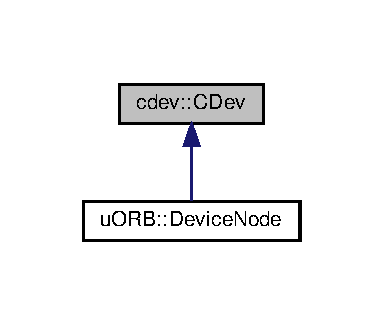
\includegraphics[width=184pt]{dc/d50/classcdev_1_1CDev__inherit__graph}
\end{center}
\end{figure}
\subsection*{Public Member Functions}
\begin{DoxyCompactItemize}
\item 
\hyperlink{classcdev_1_1CDev_acd46bce7814f428044c0258f8d0518ab}{C\+Dev} (const char $\ast$devname)
\item 
\mbox{\Hypertarget{classcdev_1_1CDev_a23663da9547f16eaa68ee0adf568bd12}\label{classcdev_1_1CDev_a23663da9547f16eaa68ee0adf568bd12}} 
{\bfseries C\+Dev} (const \hyperlink{classcdev_1_1CDev}{cdev\+::\+C\+Dev} \&)=delete
\item 
\mbox{\Hypertarget{classcdev_1_1CDev_acd0afe1a56175f89627126c57f382a20}\label{classcdev_1_1CDev_acd0afe1a56175f89627126c57f382a20}} 
\hyperlink{classcdev_1_1CDev}{C\+Dev} \& {\bfseries operator=} (const \hyperlink{classcdev_1_1CDev}{C\+Dev} \&)=delete
\item 
\mbox{\Hypertarget{classcdev_1_1CDev_a37de4c22663367cb98ee75a66479c961}\label{classcdev_1_1CDev_a37de4c22663367cb98ee75a66479c961}} 
{\bfseries C\+Dev} (\hyperlink{classcdev_1_1CDev}{C\+Dev} \&\&)=delete
\item 
\mbox{\Hypertarget{classcdev_1_1CDev_aa59b53a58372869bbe2f163bef0d5b74}\label{classcdev_1_1CDev_aa59b53a58372869bbe2f163bef0d5b74}} 
\hyperlink{classcdev_1_1CDev}{C\+Dev} \& {\bfseries operator=} (\hyperlink{classcdev_1_1CDev}{C\+Dev} \&\&)=delete
\item 
\mbox{\Hypertarget{classcdev_1_1CDev_a09c11095ecdc3b1bfe7eb0e7d47ea954}\label{classcdev_1_1CDev_a09c11095ecdc3b1bfe7eb0e7d47ea954}} 
virtual int {\bfseries init} ()
\item 
virtual int \hyperlink{classcdev_1_1CDev_ac04b7ee91373c86545107e3467ba54c1}{open} (file $\ast$filep)
\item 
virtual int \hyperlink{classcdev_1_1CDev_a9241755ab3abf102eea85dad1e3dc6c4}{close} (file $\ast$filep)
\item 
virtual ssize\+\_\+t \hyperlink{classcdev_1_1CDev_a1b0db49c478b621333aff6bb3321d057}{read} (file $\ast$filep, char $\ast$buffer, size\+\_\+t buflen)
\item 
virtual ssize\+\_\+t \hyperlink{classcdev_1_1CDev_a54aff43049b22cea19f8cc31cb2a0fd0}{write} (file $\ast$filep, const char $\ast$buffer, size\+\_\+t buflen)
\item 
virtual off\+\_\+t \hyperlink{classcdev_1_1CDev_a987dd32ef79c2bb4380fa021ce430de2}{seek} (file $\ast$filep, off\+\_\+t offset, int whence)
\item 
virtual int \hyperlink{classcdev_1_1CDev_a87eb4d4b92a501de458736e8d24eec40}{ioctl} (file $\ast$filep, int cmd, unsigned long arg)
\item 
int \hyperlink{classcdev_1_1CDev_a219a565bb1842c62e0f45a7eeaaec0d3}{poll} (file $\ast$filep, struct pollfd $\ast$fds, bool setup)
\item 
const char $\ast$ \hyperlink{classcdev_1_1CDev_a0bc1072e967a90dfac04a1227f200f6f}{get\+\_\+devname} () const
\end{DoxyCompactItemize}
\subsection*{Protected Member Functions}
\begin{DoxyCompactItemize}
\item 
virtual pollevent\+\_\+t \hyperlink{classcdev_1_1CDev_abf40a822665b0889584268e8a4dfbef2}{poll\+\_\+state} (file $\ast$filep)
\item 
void \hyperlink{classcdev_1_1CDev_aa23e0fac4d51f7b14db7a7e7dfa0ac06}{poll\+\_\+notify} (pollevent\+\_\+t events)
\item 
virtual void \hyperlink{classcdev_1_1CDev_ada35d652d0f6d7257fffe4ead0fbb6dd}{poll\+\_\+notify\+\_\+one} (struct pollfd $\ast$fds, pollevent\+\_\+t events)
\item 
virtual int \hyperlink{classcdev_1_1CDev_a89860de90cb8850c1ac71ec59764cf46}{open\+\_\+first} (file $\ast$filep)
\item 
virtual int \hyperlink{classcdev_1_1CDev_ae2fb43c7b0884dcbc6fbf1aa90d50a38}{close\+\_\+last} (file $\ast$filep)
\item 
int \hyperlink{classcdev_1_1CDev_a8cdc695d86a00139e11b2d57974475b4}{register\+\_\+class\+\_\+devname} (const char $\ast$class\+\_\+devname)
\item 
int \hyperlink{classcdev_1_1CDev_a84f73216813a23f91cd9414262484f3f}{unregister\+\_\+class\+\_\+devname} (const char $\ast$class\+\_\+devname, unsigned class\+\_\+instance)
\item 
void \hyperlink{classcdev_1_1CDev_ae676cccee31dd393ab681414a146d868}{lock} ()
\item 
void \hyperlink{classcdev_1_1CDev_af65273e0578b277deea057dc7d558e9d}{unlock} ()
\item 
int \hyperlink{classcdev_1_1CDev_a9fe9c784053bc2b7748db1ec405ae83f}{unregister\+\_\+driver\+\_\+and\+\_\+memory} ()
\end{DoxyCompactItemize}
\subsection*{Protected Attributes}
\begin{DoxyCompactItemize}
\item 
sem\+\_\+t \hyperlink{classcdev_1_1CDev_aa9b327dcb42b1160c01417ad64cd8e2b}{\+\_\+lock}
\end{DoxyCompactItemize}
\subsection*{Static Protected Attributes}
\begin{DoxyCompactItemize}
\item 
static const file\+\_\+operations \hyperlink{classcdev_1_1CDev_acb99fb0026b3466f200feef27046d612}{fops}
\end{DoxyCompactItemize}


\subsection{Detailed Description}
Abstract class for any character device 

Definition at line 77 of file C\+Dev.\+hpp.



\subsection{Constructor \& Destructor Documentation}
\mbox{\Hypertarget{classcdev_1_1CDev_acd46bce7814f428044c0258f8d0518ab}\label{classcdev_1_1CDev_acd46bce7814f428044c0258f8d0518ab}} 
\index{cdev\+::\+C\+Dev@{cdev\+::\+C\+Dev}!C\+Dev@{C\+Dev}}
\index{C\+Dev@{C\+Dev}!cdev\+::\+C\+Dev@{cdev\+::\+C\+Dev}}
\subsubsection{\texorpdfstring{C\+Dev()}{CDev()}}
{\footnotesize\ttfamily cdev\+::\+C\+Dev\+::\+C\+Dev (\begin{DoxyParamCaption}\item[{const char $\ast$}]{devname }\end{DoxyParamCaption})\hspace{0.3cm}{\ttfamily [explicit]}}

Constructor


\begin{DoxyParams}{Parameters}
{\em name} & Driver name \\
\hline
{\em devname} & Device node name \\
\hline
\end{DoxyParams}


Definition at line 59 of file C\+Dev.\+cpp.


\begin{DoxyCode}
59                               :
60     \_devname(devname)
61 \{
62     \textcolor{comment}{//PX4\_DEBUG("CDev::CDev");}
63 
64     \textcolor{keywordtype}{int} ret = sem\_init(&\hyperlink{classcdev_1_1CDev_aa9b327dcb42b1160c01417ad64cd8e2b}{\_lock}, 0, 1);
65 
66     \textcolor{keywordflow}{if} (ret != 0) \{
67         \textcolor{comment}{//PX4\_DEBUG("SEM INIT FAIL: ret %d", ret);}
68     \}
69 \}
\end{DoxyCode}


\subsection{Member Function Documentation}
\mbox{\Hypertarget{classcdev_1_1CDev_a9241755ab3abf102eea85dad1e3dc6c4}\label{classcdev_1_1CDev_a9241755ab3abf102eea85dad1e3dc6c4}} 
\index{cdev\+::\+C\+Dev@{cdev\+::\+C\+Dev}!close@{close}}
\index{close@{close}!cdev\+::\+C\+Dev@{cdev\+::\+C\+Dev}}
\subsubsection{\texorpdfstring{close()}{close()}}
{\footnotesize\ttfamily int cdev\+::\+C\+Dev\+::close (\begin{DoxyParamCaption}\item[{file $\ast$}]{filep }\end{DoxyParamCaption})\hspace{0.3cm}{\ttfamily [virtual]}}

Handle a close of the device.

This function is called for every close of the device. The default implementation maintains \+\_\+open\+\_\+count and returns OK as long as it is not zero.


\begin{DoxyParams}{Parameters}
{\em filep} & Pointer to the NuttX file structure. \\
\hline
\end{DoxyParams}
\begin{DoxyReturn}{Returns}
OK if the close was successful, -\/errno otherwise. 
\end{DoxyReturn}


Reimplemented in \hyperlink{classuORB_1_1DeviceNode_a80ebf695636c701d3378525b6d0e4148}{u\+O\+R\+B\+::\+Device\+Node}.



Definition at line 175 of file C\+Dev.\+cpp.


\begin{DoxyCode}
176 \{
177     \textcolor{comment}{//PX4\_DEBUG("CDev::close");}
178     \textcolor{keywordtype}{int} ret = 0;
179 
180     \hyperlink{classcdev_1_1CDev_ae676cccee31dd393ab681414a146d868}{lock}();
181 
182     \textcolor{keywordflow}{if} (\_open\_count > 0) \{
183         \textcolor{comment}{/* decrement the open count */}
184         \_open\_count--;
185 
186         \textcolor{comment}{/* callback cannot decline the close */}
187         \textcolor{keywordflow}{if} (\_open\_count == 0) \{
188             ret = \hyperlink{classcdev_1_1CDev_ae2fb43c7b0884dcbc6fbf1aa90d50a38}{close\_last}(filep);
189         \}
190 
191     \} \textcolor{keywordflow}{else} \{
192         ret = -EBADF;
193     \}
194 
195     \hyperlink{classcdev_1_1CDev_af65273e0578b277deea057dc7d558e9d}{unlock}();
196 
197     \textcolor{keywordflow}{return} ret;
198 \}
\end{DoxyCode}
\mbox{\Hypertarget{classcdev_1_1CDev_ae2fb43c7b0884dcbc6fbf1aa90d50a38}\label{classcdev_1_1CDev_ae2fb43c7b0884dcbc6fbf1aa90d50a38}} 
\index{cdev\+::\+C\+Dev@{cdev\+::\+C\+Dev}!close\+\_\+last@{close\+\_\+last}}
\index{close\+\_\+last@{close\+\_\+last}!cdev\+::\+C\+Dev@{cdev\+::\+C\+Dev}}
\subsubsection{\texorpdfstring{close\+\_\+last()}{close\_last()}}
{\footnotesize\ttfamily virtual int cdev\+::\+C\+Dev\+::close\+\_\+last (\begin{DoxyParamCaption}\item[{file $\ast$}]{filep }\end{DoxyParamCaption})\hspace{0.3cm}{\ttfamily [inline]}, {\ttfamily [protected]}, {\ttfamily [virtual]}}

Notification of the last close.

This function is called when the device open count transitions from one to zero. The driver lock is held for the duration of the call.

The default implementation returns OK.


\begin{DoxyParams}{Parameters}
{\em filep} & Pointer to the NuttX file structure. \\
\hline
\end{DoxyParams}
\begin{DoxyReturn}{Returns}
OK if the open should return OK, -\/errno otherwise. 
\end{DoxyReturn}


Definition at line 253 of file C\+Dev.\+hpp.


\begin{DoxyCode}
253 \{ \textcolor{keywordflow}{return} 0; \}
\end{DoxyCode}
\mbox{\Hypertarget{classcdev_1_1CDev_a0bc1072e967a90dfac04a1227f200f6f}\label{classcdev_1_1CDev_a0bc1072e967a90dfac04a1227f200f6f}} 
\index{cdev\+::\+C\+Dev@{cdev\+::\+C\+Dev}!get\+\_\+devname@{get\+\_\+devname}}
\index{get\+\_\+devname@{get\+\_\+devname}!cdev\+::\+C\+Dev@{cdev\+::\+C\+Dev}}
\subsubsection{\texorpdfstring{get\+\_\+devname()}{get\_devname()}}
{\footnotesize\ttfamily const char$\ast$ cdev\+::\+C\+Dev\+::get\+\_\+devname (\begin{DoxyParamCaption}{ }\end{DoxyParamCaption}) const\hspace{0.3cm}{\ttfamily [inline]}}

Get the device name.

\begin{DoxyReturn}{Returns}
the file system string of the device handle 
\end{DoxyReturn}


Definition at line 188 of file C\+Dev.\+hpp.


\begin{DoxyCode}
188 \{ \textcolor{keywordflow}{return} \_devname; \}
\end{DoxyCode}
\mbox{\Hypertarget{classcdev_1_1CDev_a87eb4d4b92a501de458736e8d24eec40}\label{classcdev_1_1CDev_a87eb4d4b92a501de458736e8d24eec40}} 
\index{cdev\+::\+C\+Dev@{cdev\+::\+C\+Dev}!ioctl@{ioctl}}
\index{ioctl@{ioctl}!cdev\+::\+C\+Dev@{cdev\+::\+C\+Dev}}
\subsubsection{\texorpdfstring{ioctl()}{ioctl()}}
{\footnotesize\ttfamily virtual int cdev\+::\+C\+Dev\+::ioctl (\begin{DoxyParamCaption}\item[{file $\ast$}]{filep,  }\item[{int}]{cmd,  }\item[{unsigned long}]{arg }\end{DoxyParamCaption})\hspace{0.3cm}{\ttfamily [inline]}, {\ttfamily [virtual]}}

Perform an ioctl operation on the device.

The default implementation returns -\/\+E\+N\+O\+T\+TY. Subclasses should call the default implementation for any command they do not handle themselves.


\begin{DoxyParams}{Parameters}
{\em filep} & Pointer to the NuttX file structure. \\
\hline
{\em cmd} & The ioctl command value. \\
\hline
{\em arg} & The ioctl argument value. \\
\hline
\end{DoxyParams}
\begin{DoxyReturn}{Returns}
OK on success, or -\/errno otherwise. 
\end{DoxyReturn}


Reimplemented in \hyperlink{classuORB_1_1DeviceNode_acad1520dfb19e9449546dad7a4129c26}{u\+O\+R\+B\+::\+Device\+Node}.



Definition at line 168 of file C\+Dev.\+hpp.


\begin{DoxyCode}
168 \{ \textcolor{keywordflow}{return} -ENOTTY; \};
\end{DoxyCode}
\mbox{\Hypertarget{classcdev_1_1CDev_ae676cccee31dd393ab681414a146d868}\label{classcdev_1_1CDev_ae676cccee31dd393ab681414a146d868}} 
\index{cdev\+::\+C\+Dev@{cdev\+::\+C\+Dev}!lock@{lock}}
\index{lock@{lock}!cdev\+::\+C\+Dev@{cdev\+::\+C\+Dev}}
\subsubsection{\texorpdfstring{lock()}{lock()}}
{\footnotesize\ttfamily void cdev\+::\+C\+Dev\+::lock (\begin{DoxyParamCaption}{ }\end{DoxyParamCaption})\hspace{0.3cm}{\ttfamily [inline]}, {\ttfamily [protected]}}

Take the driver lock.

Each driver instance has its own lock/semaphore.

Note that we must loop as the wait may be interrupted by a signal.

Careful\+: \hyperlink{classcdev_1_1CDev_ae676cccee31dd393ab681414a146d868}{lock()} calls cannot be nested! 

Definition at line 283 of file C\+Dev.\+hpp.


\begin{DoxyCode}
283 \{ \textcolor{keywordflow}{do} \{\} \textcolor{keywordflow}{while} (sem\_wait(&\hyperlink{classcdev_1_1CDev_aa9b327dcb42b1160c01417ad64cd8e2b}{\_lock}) != 0); \}
\end{DoxyCode}
\mbox{\Hypertarget{classcdev_1_1CDev_ac04b7ee91373c86545107e3467ba54c1}\label{classcdev_1_1CDev_ac04b7ee91373c86545107e3467ba54c1}} 
\index{cdev\+::\+C\+Dev@{cdev\+::\+C\+Dev}!open@{open}}
\index{open@{open}!cdev\+::\+C\+Dev@{cdev\+::\+C\+Dev}}
\subsubsection{\texorpdfstring{open()}{open()}}
{\footnotesize\ttfamily int cdev\+::\+C\+Dev\+::open (\begin{DoxyParamCaption}\item[{file $\ast$}]{filep }\end{DoxyParamCaption})\hspace{0.3cm}{\ttfamily [virtual]}}

Handle an open of the device.

This function is called for every open of the device. The default implementation maintains \+\_\+open\+\_\+count and always returns OK.


\begin{DoxyParams}{Parameters}
{\em filep} & Pointer to the NuttX file structure. \\
\hline
\end{DoxyParams}
\begin{DoxyReturn}{Returns}
OK if the open is allowed, -\/errno otherwise. 
\end{DoxyReturn}


Reimplemented in \hyperlink{classuORB_1_1DeviceNode_ae7f3782c9876a17b4aa6949440655f1f}{u\+O\+R\+B\+::\+Device\+Node}.



Definition at line 150 of file C\+Dev.\+cpp.


\begin{DoxyCode}
151 \{
152     \textcolor{comment}{//PX4\_DEBUG("CDev::open");}
153     \textcolor{keywordtype}{int} ret = 0;
154 
155     \hyperlink{classcdev_1_1CDev_ae676cccee31dd393ab681414a146d868}{lock}();
156     \textcolor{comment}{/* increment the open count */}
157     \_open\_count++;
158 
159     \textcolor{keywordflow}{if} (\_open\_count == 1) \{
160 
161         \textcolor{comment}{/* first-open callback may decline the open */}
162         ret = \hyperlink{classcdev_1_1CDev_a89860de90cb8850c1ac71ec59764cf46}{open\_first}(filep);
163 
164         \textcolor{keywordflow}{if} (ret != 0) \{
165             \_open\_count--;
166         \}
167     \}
168 
169     \hyperlink{classcdev_1_1CDev_af65273e0578b277deea057dc7d558e9d}{unlock}();
170 
171     \textcolor{keywordflow}{return} ret;
172 \}
\end{DoxyCode}
\mbox{\Hypertarget{classcdev_1_1CDev_a89860de90cb8850c1ac71ec59764cf46}\label{classcdev_1_1CDev_a89860de90cb8850c1ac71ec59764cf46}} 
\index{cdev\+::\+C\+Dev@{cdev\+::\+C\+Dev}!open\+\_\+first@{open\+\_\+first}}
\index{open\+\_\+first@{open\+\_\+first}!cdev\+::\+C\+Dev@{cdev\+::\+C\+Dev}}
\subsubsection{\texorpdfstring{open\+\_\+first()}{open\_first()}}
{\footnotesize\ttfamily virtual int cdev\+::\+C\+Dev\+::open\+\_\+first (\begin{DoxyParamCaption}\item[{file $\ast$}]{filep }\end{DoxyParamCaption})\hspace{0.3cm}{\ttfamily [inline]}, {\ttfamily [protected]}, {\ttfamily [virtual]}}

Notification of the first open.

This function is called when the device open count transitions from zero to one. The driver lock is held for the duration of the call.

The default implementation returns OK.


\begin{DoxyParams}{Parameters}
{\em filep} & Pointer to the NuttX file structure. \\
\hline
\end{DoxyParams}
\begin{DoxyReturn}{Returns}
OK if the open should proceed, -\/errno otherwise. 
\end{DoxyReturn}


Definition at line 240 of file C\+Dev.\+hpp.


\begin{DoxyCode}
240 \{ \textcolor{keywordflow}{return} 0; \}
\end{DoxyCode}
\mbox{\Hypertarget{classcdev_1_1CDev_a219a565bb1842c62e0f45a7eeaaec0d3}\label{classcdev_1_1CDev_a219a565bb1842c62e0f45a7eeaaec0d3}} 
\index{cdev\+::\+C\+Dev@{cdev\+::\+C\+Dev}!poll@{poll}}
\index{poll@{poll}!cdev\+::\+C\+Dev@{cdev\+::\+C\+Dev}}
\subsubsection{\texorpdfstring{poll()}{poll()}}
{\footnotesize\ttfamily int cdev\+::\+C\+Dev\+::poll (\begin{DoxyParamCaption}\item[{file $\ast$}]{filep,  }\item[{struct pollfd $\ast$}]{fds,  }\item[{bool}]{setup }\end{DoxyParamCaption})}

Perform a poll setup/teardown operation.

This is handled internally and should not normally be overridden.


\begin{DoxyParams}{Parameters}
{\em filep} & Pointer to the internal file structure. \\
\hline
{\em fds} & Poll descriptor being waited on. \\
\hline
{\em setup} & True if this is establishing a request, false if it is being torn down. \\
\hline
\end{DoxyParams}
\begin{DoxyReturn}{Returns}
OK on success, or -\/errno otherwise. 
\end{DoxyReturn}


Definition at line 201 of file C\+Dev.\+cpp.


\begin{DoxyCode}
202 \{
203     \textcolor{comment}{//PX4\_DEBUG("CDev::Poll %s", setup ? "setup" : "teardown");}
204     \textcolor{keywordtype}{int} ret = 0;
205 
206     \textcolor{keywordflow}{if} (setup) \{
207         \textcolor{comment}{/*}
208 \textcolor{comment}{         * Save the file pointer in the pollfd for the subclass'}
209 \textcolor{comment}{         * benefit.}
210 \textcolor{comment}{         */}
211         fds->priv = (\textcolor{keywordtype}{void} *)filep;
212         \textcolor{comment}{//PX4\_DEBUG("CDev::poll: fds->priv = %p", filep);}
213 
214         \textcolor{comment}{/*}
215 \textcolor{comment}{         * Lock against poll\_notify() and possibly other callers (protect \_pollset).}
216 \textcolor{comment}{         */}
217         
218         ATOMIC\_ENTER;
219 
220         \textcolor{comment}{/*}
221 \textcolor{comment}{         * Try to store the fds for later use and handle array resizing.}
222 \textcolor{comment}{         */}
223         \textcolor{keywordflow}{while} ((ret = store\_poll\_waiter(fds)) == -ENFILE) \{
224 
225             \textcolor{comment}{// No free slot found. Resize the pollset. This is expensive, but it's only needed initially.}
226 
227             \textcolor{keywordflow}{if} (\_max\_pollwaiters >= 256 / 2) \{ \textcolor{comment}{//\_max\_pollwaiters is uint8\_t}
228                 ret = -ENOMEM;
229                 \textcolor{keywordflow}{break};
230             \}
231 
232             \textcolor{keyword}{const} uint8\_t new\_count = \_max\_pollwaiters > 0 ? \_max\_pollwaiters * 2 : 1;
233             pollfd **prev\_pollset = \_pollset;
234 
235 
236             \textcolor{comment}{// malloc uses a semaphore, we need to call it enabled IRQ's}
237             leave\_critical\_section(flags);
238 
239             pollfd **new\_pollset = \textcolor{keyword}{new} pollfd *[new\_count];
240 
241 
242             flags = enter\_critical\_section();
243 
244 
245             \textcolor{keywordflow}{if} (prev\_pollset == \_pollset) \{
246                 \textcolor{comment}{// no one else updated the \_pollset meanwhile, so we're good to go}
247                 \textcolor{keywordflow}{if} (!new\_pollset) \{
248                     ret = -ENOMEM;
249                     \textcolor{keywordflow}{break};
250                 \}
251 
252                 \textcolor{keywordflow}{if} (\_max\_pollwaiters > 0) \{
253                     memset(new\_pollset + \_max\_pollwaiters, 0, \textcolor{keyword}{sizeof}(pollfd *) * (new\_count - 
      \_max\_pollwaiters));
254                     memcpy(new\_pollset, \_pollset, \textcolor{keyword}{sizeof}(pollfd *) * \_max\_pollwaiters);
255                 \}
256 
257                 \_pollset = new\_pollset;
258                 \_pollset[\_max\_pollwaiters] = fds;
259                 \_max\_pollwaiters = new\_count;
260 
261                 \textcolor{comment}{// free the previous \_pollset (we need to unlock here which is fine because we don't access
       \_pollset anymore)}
262 
263                 leave\_critical\_section(flags);
264 
265 
266                 \textcolor{keywordflow}{if} (prev\_pollset) \{
267                     \textcolor{keyword}{delete}[](prev\_pollset);
268                 \}
269 
270 
271                 flags = enter\_critical\_section();
272 
273 
274                 \textcolor{comment}{// Success}
275                 ret = 0;
276                 \textcolor{keywordflow}{break};
277             \}
278 
279 
280             leave\_critical\_section(flags);
281 
282             \textcolor{comment}{// We have to retry}
283             \textcolor{keyword}{delete}[] new\_pollset;
284 
285             flags = enter\_critical\_section();
286 
287         \}
288 
289         \textcolor{keywordflow}{if} (ret == 0) \{
290 
291             \textcolor{comment}{/*}
292 \textcolor{comment}{             * Check to see whether we should send a poll notification}
293 \textcolor{comment}{             * immediately.}
294 \textcolor{comment}{             */}
295             fds->revents |= fds->events & \hyperlink{classcdev_1_1CDev_abf40a822665b0889584268e8a4dfbef2}{poll\_state}(filep);
296 
297             \textcolor{comment}{/* yes? post the notification */}
298             \textcolor{keywordflow}{if} (fds->revents != 0) \{
299                 sem\_post(fds->sem);
300             \}
301 
302         \}
303 
304         ATOMIC\_LEAVE;
305 
306     \} \textcolor{keywordflow}{else} \{
307         ATOMIC\_ENTER;
308         \textcolor{comment}{/*}
309 \textcolor{comment}{         * Handle a teardown request.}
310 \textcolor{comment}{         */}
311         ret = remove\_poll\_waiter(fds);
312         ATOMIC\_LEAVE;
313     \}
314 
315     \textcolor{keywordflow}{return} ret;
316 \}
\end{DoxyCode}
\mbox{\Hypertarget{classcdev_1_1CDev_aa23e0fac4d51f7b14db7a7e7dfa0ac06}\label{classcdev_1_1CDev_aa23e0fac4d51f7b14db7a7e7dfa0ac06}} 
\index{cdev\+::\+C\+Dev@{cdev\+::\+C\+Dev}!poll\+\_\+notify@{poll\+\_\+notify}}
\index{poll\+\_\+notify@{poll\+\_\+notify}!cdev\+::\+C\+Dev@{cdev\+::\+C\+Dev}}
\subsubsection{\texorpdfstring{poll\+\_\+notify()}{poll\_notify()}}
{\footnotesize\ttfamily void cdev\+::\+C\+Dev\+::poll\+\_\+notify (\begin{DoxyParamCaption}\item[{pollevent\+\_\+t}]{events }\end{DoxyParamCaption})\hspace{0.3cm}{\ttfamily [protected]}}

Report new poll events.

This function should be called anytime the state of the device changes in a fashion that might be interesting to a poll waiter.


\begin{DoxyParams}{Parameters}
{\em events} & The new event(s) being announced. \\
\hline
\end{DoxyParams}


Definition at line 319 of file C\+Dev.\+cpp.


\begin{DoxyCode}
320 \{
321     \textcolor{comment}{//PX4\_DEBUG("CDev::poll\_notify events = %0x", events);}
322 
323     \textcolor{comment}{/* lock against poll() as well as other wakeups */}
324     ATOMIC\_ENTER;
325 
326     \textcolor{keywordflow}{for} (\textcolor{keywordtype}{unsigned} i = 0; i < \_max\_pollwaiters; i++) \{
327         \textcolor{keywordflow}{if} (\textcolor{keyword}{nullptr} != \_pollset[i]) \{
328             \hyperlink{classcdev_1_1CDev_ada35d652d0f6d7257fffe4ead0fbb6dd}{poll\_notify\_one}(\_pollset[i], events);
329         \}
330     \}
331 
332     ATOMIC\_LEAVE;
333 \}
\end{DoxyCode}
\mbox{\Hypertarget{classcdev_1_1CDev_ada35d652d0f6d7257fffe4ead0fbb6dd}\label{classcdev_1_1CDev_ada35d652d0f6d7257fffe4ead0fbb6dd}} 
\index{cdev\+::\+C\+Dev@{cdev\+::\+C\+Dev}!poll\+\_\+notify\+\_\+one@{poll\+\_\+notify\+\_\+one}}
\index{poll\+\_\+notify\+\_\+one@{poll\+\_\+notify\+\_\+one}!cdev\+::\+C\+Dev@{cdev\+::\+C\+Dev}}
\subsubsection{\texorpdfstring{poll\+\_\+notify\+\_\+one()}{poll\_notify\_one()}}
{\footnotesize\ttfamily void cdev\+::\+C\+Dev\+::poll\+\_\+notify\+\_\+one (\begin{DoxyParamCaption}\item[{struct pollfd $\ast$}]{fds,  }\item[{pollevent\+\_\+t}]{events }\end{DoxyParamCaption})\hspace{0.3cm}{\ttfamily [protected]}, {\ttfamily [virtual]}}

Internal implementation of poll\+\_\+notify.


\begin{DoxyParams}{Parameters}
{\em fds} & A poll waiter to notify. \\
\hline
{\em events} & The event(s) to send to the waiter. \\
\hline
\end{DoxyParams}


Reimplemented in \hyperlink{classuORB_1_1DeviceNode_a77061c03defdcb3eedfc9cdc8b38c003}{u\+O\+R\+B\+::\+Device\+Node}.



Definition at line 336 of file C\+Dev.\+cpp.


\begin{DoxyCode}
337 \{
338     \textcolor{comment}{//PX4\_DEBUG("CDev::poll\_notify\_one");}
339 
340     \textcolor{comment}{/* update the reported event set */}
341     fds->revents |= fds->events & events;
342 
343     \textcolor{comment}{//PX4\_DEBUG(" Events fds=%p %0x %0x %0x", fds, fds->revents, fds->events, events);}
344 
345     \textcolor{keywordflow}{if} (fds->revents != 0) \{
346         sem\_post(fds->sem);
347     \}
348 \}
\end{DoxyCode}
\mbox{\Hypertarget{classcdev_1_1CDev_abf40a822665b0889584268e8a4dfbef2}\label{classcdev_1_1CDev_abf40a822665b0889584268e8a4dfbef2}} 
\index{cdev\+::\+C\+Dev@{cdev\+::\+C\+Dev}!poll\+\_\+state@{poll\+\_\+state}}
\index{poll\+\_\+state@{poll\+\_\+state}!cdev\+::\+C\+Dev@{cdev\+::\+C\+Dev}}
\subsubsection{\texorpdfstring{poll\+\_\+state()}{poll\_state()}}
{\footnotesize\ttfamily virtual pollevent\+\_\+t cdev\+::\+C\+Dev\+::poll\+\_\+state (\begin{DoxyParamCaption}\item[{file $\ast$}]{filep }\end{DoxyParamCaption})\hspace{0.3cm}{\ttfamily [inline]}, {\ttfamily [protected]}, {\ttfamily [virtual]}}

Check the current state of the device for poll events from the perspective of the file.

This function is called by the default \hyperlink{classcdev_1_1CDev_a219a565bb1842c62e0f45a7eeaaec0d3}{poll()} implementation when a poll is set up to determine whether the poll should return immediately.

The default implementation returns no events.


\begin{DoxyParams}{Parameters}
{\em filep} & The file that\textquotesingle{}s interested. \\
\hline
\end{DoxyParams}
\begin{DoxyReturn}{Returns}
The current set of poll events. 
\end{DoxyReturn}


Reimplemented in \hyperlink{classuORB_1_1DeviceNode_a3ac7d5c93e5fd480cd623fd421afa060}{u\+O\+R\+B\+::\+Device\+Node}.



Definition at line 209 of file C\+Dev.\+hpp.


\begin{DoxyCode}
209 \{ \textcolor{keywordflow}{return} 0; \}
\end{DoxyCode}
\mbox{\Hypertarget{classcdev_1_1CDev_a1b0db49c478b621333aff6bb3321d057}\label{classcdev_1_1CDev_a1b0db49c478b621333aff6bb3321d057}} 
\index{cdev\+::\+C\+Dev@{cdev\+::\+C\+Dev}!read@{read}}
\index{read@{read}!cdev\+::\+C\+Dev@{cdev\+::\+C\+Dev}}
\subsubsection{\texorpdfstring{read()}{read()}}
{\footnotesize\ttfamily virtual ssize\+\_\+t cdev\+::\+C\+Dev\+::read (\begin{DoxyParamCaption}\item[{file $\ast$}]{filep,  }\item[{char $\ast$}]{buffer,  }\item[{size\+\_\+t}]{buflen }\end{DoxyParamCaption})\hspace{0.3cm}{\ttfamily [inline]}, {\ttfamily [virtual]}}

Perform a read from the device.

The default implementation returns -\/\+E\+N\+O\+S\+YS.


\begin{DoxyParams}{Parameters}
{\em filep} & Pointer to the NuttX file structure. \\
\hline
{\em buffer} & Pointer to the buffer into which data should be placed. \\
\hline
{\em buflen} & The number of bytes to be read. \\
\hline
\end{DoxyParams}
\begin{DoxyReturn}{Returns}
The number of bytes read or -\/errno otherwise. 
\end{DoxyReturn}


Reimplemented in \hyperlink{classuORB_1_1DeviceNode_ada5db18aae221ae76e023651cbf9461c}{u\+O\+R\+B\+::\+Device\+Node}.



Definition at line 130 of file C\+Dev.\+hpp.


\begin{DoxyCode}
130 \{ \textcolor{keywordflow}{return} -ENOSYS; \}
\end{DoxyCode}
\mbox{\Hypertarget{classcdev_1_1CDev_a8cdc695d86a00139e11b2d57974475b4}\label{classcdev_1_1CDev_a8cdc695d86a00139e11b2d57974475b4}} 
\index{cdev\+::\+C\+Dev@{cdev\+::\+C\+Dev}!register\+\_\+class\+\_\+devname@{register\+\_\+class\+\_\+devname}}
\index{register\+\_\+class\+\_\+devname@{register\+\_\+class\+\_\+devname}!cdev\+::\+C\+Dev@{cdev\+::\+C\+Dev}}
\subsubsection{\texorpdfstring{register\+\_\+class\+\_\+devname()}{register\_class\_devname()}}
{\footnotesize\ttfamily int cdev\+::\+C\+Dev\+::register\+\_\+class\+\_\+devname (\begin{DoxyParamCaption}\item[{const char $\ast$}]{class\+\_\+devname }\end{DoxyParamCaption})\hspace{0.3cm}{\ttfamily [protected]}}

Register a class device name, automatically adding device class instance suffix if need be.


\begin{DoxyParams}{Parameters}
{\em class\+\_\+devname} & Device class name \\
\hline
\end{DoxyParams}
\begin{DoxyReturn}{Returns}
class\+\_\+instamce Class instance created, or -\/errno on failure 
\end{DoxyReturn}


Definition at line 87 of file C\+Dev.\+cpp.


\begin{DoxyCode}
88 \{
89     \textcolor{comment}{//PX4\_DEBUG("CDev::register\_class\_devname %s", class\_devname);}
90 
91     \textcolor{keywordflow}{if} (class\_devname == \textcolor{keyword}{nullptr}) \{
92         \textcolor{keywordflow}{return} -EINVAL;
93     \}
94 
95     \textcolor{keywordtype}{int} class\_instance = 0;
96     \textcolor{keywordtype}{int} ret = -ENOSPC;
97 
98     \textcolor{keywordflow}{while} (class\_instance < 4) \{
99         \textcolor{keywordtype}{char} name[32];
100         snprintf(name, \textcolor{keyword}{sizeof}(name), \textcolor{stringliteral}{"%s%d"}, class\_devname, class\_instance);
101         ret = register\_driver(name, &\hyperlink{classcdev_1_1CDev_acb99fb0026b3466f200feef27046d612}{fops}, 0666, (\textcolor{keywordtype}{void} *)\textcolor{keyword}{this});
102 
103         \textcolor{keywordflow}{if} (ret == 0) \{
104             \textcolor{keywordflow}{break};
105         \}
106 
107         class\_instance++;
108     \}
109 
110     \textcolor{keywordflow}{if} (class\_instance == 4) \{
111         \textcolor{keywordflow}{return} ret;
112     \}
113 
114     \textcolor{keywordflow}{return} class\_instance;
115 \}
\end{DoxyCode}
\mbox{\Hypertarget{classcdev_1_1CDev_a987dd32ef79c2bb4380fa021ce430de2}\label{classcdev_1_1CDev_a987dd32ef79c2bb4380fa021ce430de2}} 
\index{cdev\+::\+C\+Dev@{cdev\+::\+C\+Dev}!seek@{seek}}
\index{seek@{seek}!cdev\+::\+C\+Dev@{cdev\+::\+C\+Dev}}
\subsubsection{\texorpdfstring{seek()}{seek()}}
{\footnotesize\ttfamily virtual off\+\_\+t cdev\+::\+C\+Dev\+::seek (\begin{DoxyParamCaption}\item[{file $\ast$}]{filep,  }\item[{off\+\_\+t}]{offset,  }\item[{int}]{whence }\end{DoxyParamCaption})\hspace{0.3cm}{\ttfamily [inline]}, {\ttfamily [virtual]}}

Perform a logical seek operation on the device.

The default implementation returns -\/\+E\+N\+O\+S\+YS.


\begin{DoxyParams}{Parameters}
{\em filep} & Pointer to the NuttX file structure. \\
\hline
{\em offset} & The new file position relative to whence. \\
\hline
{\em whence} & S\+E\+E\+K\+\_\+\+O\+FS, S\+E\+E\+K\+\_\+\+C\+UR or S\+E\+E\+K\+\_\+\+E\+ND. \\
\hline
\end{DoxyParams}
\begin{DoxyReturn}{Returns}
The previous offset, or -\/errno otherwise. 
\end{DoxyReturn}


Definition at line 154 of file C\+Dev.\+hpp.


\begin{DoxyCode}
154 \{ \textcolor{keywordflow}{return} -ENOSYS; \}
\end{DoxyCode}
\mbox{\Hypertarget{classcdev_1_1CDev_af65273e0578b277deea057dc7d558e9d}\label{classcdev_1_1CDev_af65273e0578b277deea057dc7d558e9d}} 
\index{cdev\+::\+C\+Dev@{cdev\+::\+C\+Dev}!unlock@{unlock}}
\index{unlock@{unlock}!cdev\+::\+C\+Dev@{cdev\+::\+C\+Dev}}
\subsubsection{\texorpdfstring{unlock()}{unlock()}}
{\footnotesize\ttfamily void cdev\+::\+C\+Dev\+::unlock (\begin{DoxyParamCaption}{ }\end{DoxyParamCaption})\hspace{0.3cm}{\ttfamily [inline]}, {\ttfamily [protected]}}

Release the driver lock. 

Definition at line 288 of file C\+Dev.\+hpp.


\begin{DoxyCode}
288 \{ sem\_post(&\hyperlink{classcdev_1_1CDev_aa9b327dcb42b1160c01417ad64cd8e2b}{\_lock}); \}
\end{DoxyCode}
\mbox{\Hypertarget{classcdev_1_1CDev_a84f73216813a23f91cd9414262484f3f}\label{classcdev_1_1CDev_a84f73216813a23f91cd9414262484f3f}} 
\index{cdev\+::\+C\+Dev@{cdev\+::\+C\+Dev}!unregister\+\_\+class\+\_\+devname@{unregister\+\_\+class\+\_\+devname}}
\index{unregister\+\_\+class\+\_\+devname@{unregister\+\_\+class\+\_\+devname}!cdev\+::\+C\+Dev@{cdev\+::\+C\+Dev}}
\subsubsection{\texorpdfstring{unregister\+\_\+class\+\_\+devname()}{unregister\_class\_devname()}}
{\footnotesize\ttfamily int cdev\+::\+C\+Dev\+::unregister\+\_\+class\+\_\+devname (\begin{DoxyParamCaption}\item[{const char $\ast$}]{class\+\_\+devname,  }\item[{unsigned}]{class\+\_\+instance }\end{DoxyParamCaption})\hspace{0.3cm}{\ttfamily [protected]}}

Register a class device name, automatically adding device class instance suffix if need be.


\begin{DoxyParams}{Parameters}
{\em class\+\_\+devname} & Device class name \\
\hline
{\em class\+\_\+instance} & Device class instance from \hyperlink{classcdev_1_1CDev_a8cdc695d86a00139e11b2d57974475b4}{register\+\_\+class\+\_\+devname()} \\
\hline
\end{DoxyParams}
\begin{DoxyReturn}{Returns}
OK on success, -\/errno otherwise 
\end{DoxyReturn}


Definition at line 118 of file C\+Dev.\+cpp.


\begin{DoxyCode}
119 \{
120     \textcolor{comment}{//PX4\_DEBUG("CDev::unregister\_class\_devname");}
121 
122     \textcolor{keywordtype}{char} name[32];
123     snprintf(name, \textcolor{keyword}{sizeof}(name), \textcolor{stringliteral}{"%s%u"}, class\_devname, class\_instance);
124     \textcolor{keywordflow}{return} unregister\_driver(name);
125 \}
\end{DoxyCode}
\mbox{\Hypertarget{classcdev_1_1CDev_a9fe9c784053bc2b7748db1ec405ae83f}\label{classcdev_1_1CDev_a9fe9c784053bc2b7748db1ec405ae83f}} 
\index{cdev\+::\+C\+Dev@{cdev\+::\+C\+Dev}!unregister\+\_\+driver\+\_\+and\+\_\+memory@{unregister\+\_\+driver\+\_\+and\+\_\+memory}}
\index{unregister\+\_\+driver\+\_\+and\+\_\+memory@{unregister\+\_\+driver\+\_\+and\+\_\+memory}!cdev\+::\+C\+Dev@{cdev\+::\+C\+Dev}}
\subsubsection{\texorpdfstring{unregister\+\_\+driver\+\_\+and\+\_\+memory()}{unregister\_driver\_and\_memory()}}
{\footnotesize\ttfamily int cdev\+::\+C\+Dev\+::unregister\+\_\+driver\+\_\+and\+\_\+memory (\begin{DoxyParamCaption}{ }\end{DoxyParamCaption})\hspace{0.3cm}{\ttfamily [protected]}}

First, unregisters the driver. Next, free the memory for the devname, in case it was expected to have ownership. Sets devname to nullptr.

This is only needed if the ownership of the devname was passed to the \hyperlink{classcdev_1_1CDev}{C\+Dev}, otherwise $\sim$\+C\+Dev handles it.

\begin{DoxyReturn}{Returns}
P\+X4\+\_\+\+OK on success, -\/\+E\+N\+O\+D\+EV if the devname is already nullptr 
\end{DoxyReturn}


Definition at line 387 of file C\+Dev.\+cpp.


\begin{DoxyCode}
388 \{
389     \textcolor{keywordtype}{int} retval = 0;
390 
391     \textcolor{keywordflow}{if} (\_registered) \{
392         unregister\_driver(\_devname);
393         \_registered = \textcolor{keyword}{false};
394 
395     \} \textcolor{keywordflow}{else} \{
396         retval = -ENODEV;
397     \}
398 
399     \textcolor{keywordflow}{if} (\_devname != \textcolor{keyword}{nullptr}) \{
400         free((\textcolor{keywordtype}{void} *)\_devname);
401         \_devname = \textcolor{keyword}{nullptr};
402 
403     \} \textcolor{keywordflow}{else} \{
404         retval = -ENODEV;
405     \}
406 
407     \textcolor{keywordflow}{return} retval;
408 \}
\end{DoxyCode}
\mbox{\Hypertarget{classcdev_1_1CDev_a54aff43049b22cea19f8cc31cb2a0fd0}\label{classcdev_1_1CDev_a54aff43049b22cea19f8cc31cb2a0fd0}} 
\index{cdev\+::\+C\+Dev@{cdev\+::\+C\+Dev}!write@{write}}
\index{write@{write}!cdev\+::\+C\+Dev@{cdev\+::\+C\+Dev}}
\subsubsection{\texorpdfstring{write()}{write()}}
{\footnotesize\ttfamily virtual ssize\+\_\+t cdev\+::\+C\+Dev\+::write (\begin{DoxyParamCaption}\item[{file $\ast$}]{filep,  }\item[{const char $\ast$}]{buffer,  }\item[{size\+\_\+t}]{buflen }\end{DoxyParamCaption})\hspace{0.3cm}{\ttfamily [inline]}, {\ttfamily [virtual]}}

Perform a write to the device.

The default implementation returns -\/\+E\+N\+O\+S\+YS.


\begin{DoxyParams}{Parameters}
{\em filep} & Pointer to the NuttX file structure. \\
\hline
{\em buffer} & Pointer to the buffer from which data should be read. \\
\hline
{\em buflen} & The number of bytes to be written. \\
\hline
\end{DoxyParams}
\begin{DoxyReturn}{Returns}
The number of bytes written or -\/errno otherwise. 
\end{DoxyReturn}


Reimplemented in \hyperlink{classuORB_1_1DeviceNode_ab58b8b4b6cac9fd8aa4d90a85e044c78}{u\+O\+R\+B\+::\+Device\+Node}.



Definition at line 142 of file C\+Dev.\+hpp.


\begin{DoxyCode}
142 \{ \textcolor{keywordflow}{return} -ENOSYS; \}
\end{DoxyCode}


\subsection{Member Data Documentation}
\mbox{\Hypertarget{classcdev_1_1CDev_aa9b327dcb42b1160c01417ad64cd8e2b}\label{classcdev_1_1CDev_aa9b327dcb42b1160c01417ad64cd8e2b}} 
\index{cdev\+::\+C\+Dev@{cdev\+::\+C\+Dev}!\+\_\+lock@{\+\_\+lock}}
\index{\+\_\+lock@{\+\_\+lock}!cdev\+::\+C\+Dev@{cdev\+::\+C\+Dev}}
\subsubsection{\texorpdfstring{\+\_\+lock}{\_lock}}
{\footnotesize\ttfamily sem\+\_\+t cdev\+::\+C\+Dev\+::\+\_\+lock\hspace{0.3cm}{\ttfamily [protected]}}

lock to protect access to all class members (also for derived classes) 

Definition at line 290 of file C\+Dev.\+hpp.

\mbox{\Hypertarget{classcdev_1_1CDev_acb99fb0026b3466f200feef27046d612}\label{classcdev_1_1CDev_acb99fb0026b3466f200feef27046d612}} 
\index{cdev\+::\+C\+Dev@{cdev\+::\+C\+Dev}!fops@{fops}}
\index{fops@{fops}!cdev\+::\+C\+Dev@{cdev\+::\+C\+Dev}}
\subsubsection{\texorpdfstring{fops}{fops}}
{\footnotesize\ttfamily const file\+\_\+operations cdev\+::\+C\+Dev\+::fops\hspace{0.3cm}{\ttfamily [static]}, {\ttfamily [protected]}}

Pointer to the default cdev file operations table; useful for registering clone devices etc. 

Definition at line 195 of file C\+Dev.\+hpp.



The documentation for this class was generated from the following files\+:\begin{DoxyCompactItemize}
\item 
/home/andressanchez/\+Escritorio/\+G\+I\+T/project\+\_\+template/src/lib/cdev/\hyperlink{CDev_8hpp}{C\+Dev.\+hpp}\item 
/home/andressanchez/\+Escritorio/\+G\+I\+T/project\+\_\+template/src/lib/cdev/\hyperlink{CDev_8cpp}{C\+Dev.\+cpp}\end{DoxyCompactItemize}

\hypertarget{structcdev_1_1cdev}{}\section{cdev\+:\+:cdev Struct Reference}
\label{structcdev_1_1cdev}\index{cdev\+::cdev@{cdev\+::cdev}}


Inheritance diagram for cdev\+:\+:cdev\+:\nopagebreak
\begin{figure}[H]
\begin{center}
\leavevmode
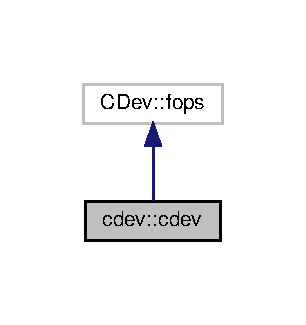
\includegraphics[width=147pt]{d6/d11/structcdev_1_1cdev__inherit__graph}
\end{center}
\end{figure}


Collaboration diagram for cdev\+:\+:cdev\+:\nopagebreak
\begin{figure}[H]
\begin{center}
\leavevmode
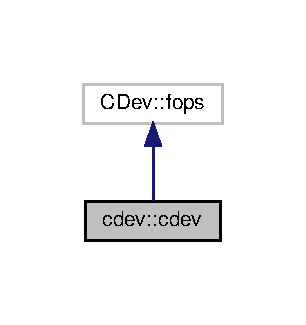
\includegraphics[width=147pt]{d9/d7b/structcdev_1_1cdev__coll__graph}
\end{center}
\end{figure}
\subsection*{Public Attributes}
\begin{DoxyCompactItemize}
\item 
\mbox{\Hypertarget{structcdev_1_1cdev_ad78a6a0e36a5cbcb65085d9f3451434a}\label{structcdev_1_1cdev_ad78a6a0e36a5cbcb65085d9f3451434a}} 
open {\bfseries \+\_\+\+\_\+pad0\+\_\+\+\_\+}\+: cdev\+\_\+open
\item 
\mbox{\Hypertarget{structcdev_1_1cdev_afa6a27c9cd18455a66b05ee250965734}\label{structcdev_1_1cdev_afa6a27c9cd18455a66b05ee250965734}} 
open {\bfseries close}\+: cdev\+\_\+close
\item 
\mbox{\Hypertarget{structcdev_1_1cdev_a34d75e9dc0cb893deb2c9ba202ac38bb}\label{structcdev_1_1cdev_a34d75e9dc0cb893deb2c9ba202ac38bb}} 
open {\bfseries read}\+: cdev\+\_\+read
\item 
\mbox{\Hypertarget{structcdev_1_1cdev_a295f01f9ecc139d92fb45ec56ce7f0c8}\label{structcdev_1_1cdev_a295f01f9ecc139d92fb45ec56ce7f0c8}} 
open {\bfseries write}\+: cdev\+\_\+write
\item 
\mbox{\Hypertarget{structcdev_1_1cdev_aa82716ece1d323b301d7405dfa1d962e}\label{structcdev_1_1cdev_aa82716ece1d323b301d7405dfa1d962e}} 
open {\bfseries seek}\+: cdev\+\_\+seek
\item 
\mbox{\Hypertarget{structcdev_1_1cdev_aa52499d86031b563c50fbfc2ff26d45a}\label{structcdev_1_1cdev_aa52499d86031b563c50fbfc2ff26d45a}} 
open {\bfseries ioctl}\+: cdev\+\_\+ioctl
\item 
\mbox{\Hypertarget{structcdev_1_1cdev_afa6c6db96c957ac3f213309995bedfdb}\label{structcdev_1_1cdev_afa6c6db96c957ac3f213309995bedfdb}} 
open {\bfseries poll}\+: cdev\+\_\+poll
\end{DoxyCompactItemize}


\subsection{Detailed Description}
Character device indirection table.

Every cdev we register gets the same function table; we use the private data field in the inode to store the instance pointer.

Note that we use the G\+NU extension syntax here because we don\textquotesingle{}t get designated initialisers in gcc 4.\+6. 

Definition at line 74 of file cdev\+\_\+platform.\+cpp.



The documentation for this struct was generated from the following file\+:\begin{DoxyCompactItemize}
\item 
/home/andressanchez/\+Escritorio/\+G\+I\+T/project\+\_\+template/src/lib/cdev/nuttx/\hyperlink{cdev__platform_8cpp}{cdev\+\_\+platform.\+cpp}\end{DoxyCompactItemize}

\hypertarget{classuORB_1_1DeviceMaster}{}\section{u\+O\+RB\+:\+:Device\+Master Class Reference}
\label{classuORB_1_1DeviceMaster}\index{u\+O\+R\+B\+::\+Device\+Master@{u\+O\+R\+B\+::\+Device\+Master}}


{\ttfamily \#include $<$u\+O\+R\+B\+Device\+Master.\+hpp$>$}

\subsection*{Public Member Functions}
\begin{DoxyCompactItemize}
\item 
\mbox{\Hypertarget{classuORB_1_1DeviceMaster_a772af4822d194e3ff6cff97da4635aa1}\label{classuORB_1_1DeviceMaster_a772af4822d194e3ff6cff97da4635aa1}} 
int {\bfseries advertise} (const struct \hyperlink{structorb__metadata}{orb\+\_\+metadata} $\ast$meta, bool is\+\_\+advertiser, int $\ast$instance)
\item 
\hyperlink{classuORB_1_1DeviceNode}{u\+O\+R\+B\+::\+Device\+Node} $\ast$ \hyperlink{classuORB_1_1DeviceMaster_a793df66a48dcabdd0f5bd8c85beee13c}{get\+Device\+Node} (const char $\ast$node\+\_\+name)
\item 
\mbox{\Hypertarget{classuORB_1_1DeviceMaster_a2ed78f9b1cded34f77423a014cbe7d8c}\label{classuORB_1_1DeviceMaster_a2ed78f9b1cded34f77423a014cbe7d8c}} 
\hyperlink{classuORB_1_1DeviceNode}{u\+O\+R\+B\+::\+Device\+Node} $\ast$ {\bfseries get\+Device\+Node} (const struct \hyperlink{structorb__metadata}{orb\+\_\+metadata} $\ast$meta, const uint8\+\_\+t instance)
\item 
\mbox{\Hypertarget{classuORB_1_1DeviceMaster_a6589533893a7c6095e69a27a25ff48ad}\label{classuORB_1_1DeviceMaster_a6589533893a7c6095e69a27a25ff48ad}} 
bool {\bfseries device\+Node\+Exists} (\hyperlink{uORB_8h_a96af5434ec1acdf24287bd7851b0413f}{O\+R\+B\+\_\+\+ID} id, const uint8\+\_\+t instance)
\item 
void \hyperlink{classuORB_1_1DeviceMaster_a0a8af69f5ba05738eb173a116acd8daf}{print\+Statistics} ()
\item 
void \hyperlink{classuORB_1_1DeviceMaster_af9f100ed05355fdd8860e27dd8876611}{show\+Top} (char $\ast$$\ast$topic\+\_\+filter, int num\+\_\+filters)
\end{DoxyCompactItemize}
\subsection*{Friends}
\begin{DoxyCompactItemize}
\item 
\mbox{\Hypertarget{classuORB_1_1DeviceMaster_ac7c1906a5bb7b0e69f9dcffc0c178300}\label{classuORB_1_1DeviceMaster_ac7c1906a5bb7b0e69f9dcffc0c178300}} 
class {\bfseries u\+O\+R\+B\+::\+Manager}
\end{DoxyCompactItemize}


\subsection{Detailed Description}
Master control device for Obj\+Dev.

Used primarily to create new objects via the O\+R\+B\+I\+O\+C\+C\+R\+E\+A\+TE ioctl. 

Definition at line 65 of file u\+O\+R\+B\+Device\+Master.\+hpp.



\subsection{Member Function Documentation}
\mbox{\Hypertarget{classuORB_1_1DeviceMaster_a793df66a48dcabdd0f5bd8c85beee13c}\label{classuORB_1_1DeviceMaster_a793df66a48dcabdd0f5bd8c85beee13c}} 
\index{u\+O\+R\+B\+::\+Device\+Master@{u\+O\+R\+B\+::\+Device\+Master}!get\+Device\+Node@{get\+Device\+Node}}
\index{get\+Device\+Node@{get\+Device\+Node}!u\+O\+R\+B\+::\+Device\+Master@{u\+O\+R\+B\+::\+Device\+Master}}
\subsubsection{\texorpdfstring{get\+Device\+Node()}{getDeviceNode()}}
{\footnotesize\ttfamily \hyperlink{classuORB_1_1DeviceNode}{u\+O\+R\+B\+::\+Device\+Node} $\ast$ u\+O\+R\+B\+::\+Device\+Master\+::get\+Device\+Node (\begin{DoxyParamCaption}\item[{const char $\ast$}]{node\+\_\+name }\end{DoxyParamCaption})}

Public interface for get\+Device\+Node\+Locked(). Takes care of synchronization. \begin{DoxyReturn}{Returns}
node if exists, nullptr otherwise 
\end{DoxyReturn}


Definition at line 417 of file u\+O\+R\+B\+Device\+Master.\+cpp.


\begin{DoxyCode}
418 \{
419     lock();
420 
421     \textcolor{keywordflow}{for} (\hyperlink{classuORB_1_1DeviceNode}{uORB::DeviceNode} *node : \_node\_list) \{
422         \textcolor{keywordflow}{if} (strcmp(node->get\_devname(), nodepath) == 0) \{
423             unlock();
424             \textcolor{keywordflow}{return} node;
425         \}
426     \}
427 
428     unlock();
429 
430     \textcolor{keywordflow}{return} \textcolor{keyword}{nullptr};
431 \}
\end{DoxyCode}
\mbox{\Hypertarget{classuORB_1_1DeviceMaster_a0a8af69f5ba05738eb173a116acd8daf}\label{classuORB_1_1DeviceMaster_a0a8af69f5ba05738eb173a116acd8daf}} 
\index{u\+O\+R\+B\+::\+Device\+Master@{u\+O\+R\+B\+::\+Device\+Master}!print\+Statistics@{print\+Statistics}}
\index{print\+Statistics@{print\+Statistics}!u\+O\+R\+B\+::\+Device\+Master@{u\+O\+R\+B\+::\+Device\+Master}}
\subsubsection{\texorpdfstring{print\+Statistics()}{printStatistics()}}
{\footnotesize\ttfamily void u\+O\+R\+B\+::\+Device\+Master\+::print\+Statistics (\begin{DoxyParamCaption}{ }\end{DoxyParamCaption})}

Print statistics for each existing topic. 

Definition at line 179 of file u\+O\+R\+B\+Device\+Master.\+cpp.


\begin{DoxyCode}
180 \{
181     \textcolor{comment}{/* Add all nodes to a list while locked, and then print them in unlocked state, to avoid potential}
182 \textcolor{comment}{     * dead-locks (where printing blocks) */}
183     lock();
184     DeviceNodeStatisticsData *first\_node = \textcolor{keyword}{nullptr};
185     DeviceNodeStatisticsData *cur\_node = \textcolor{keyword}{nullptr};
186     \textcolor{keywordtype}{size\_t} max\_topic\_name\_length = 0;
187     \textcolor{keywordtype}{int} num\_topics = 0;
188     \textcolor{keywordtype}{int} ret = addNewDeviceNodes(&first\_node, num\_topics, max\_topic\_name\_length, \textcolor{keyword}{nullptr}, 0);
189     unlock();
190 
191     \textcolor{keywordflow}{if} (ret != 0) \{
192         printf(\textcolor{stringliteral}{"addNewDeviceNodes failed (%i)"}, ret);
193         \textcolor{keywordflow}{return};
194     \}
195 
196     printf(\textcolor{stringliteral}{"%-*s INST #SUB #Q SIZE PATH\(\backslash\)n"}, (\textcolor{keywordtype}{int})max\_topic\_name\_length - 2, \textcolor{stringliteral}{"TOPIC NAME"});
197 
198     cur\_node = first\_node;
199 
200     \textcolor{keywordflow}{while} (cur\_node) \{
201         cur\_node->node->print\_statistics(max\_topic\_name\_length);
202 
203         DeviceNodeStatisticsData *prev = cur\_node;
204         cur\_node = cur\_node->next;
205         \textcolor{keyword}{delete} prev;
206     \}
207 \}
\end{DoxyCode}
\mbox{\Hypertarget{classuORB_1_1DeviceMaster_af9f100ed05355fdd8860e27dd8876611}\label{classuORB_1_1DeviceMaster_af9f100ed05355fdd8860e27dd8876611}} 
\index{u\+O\+R\+B\+::\+Device\+Master@{u\+O\+R\+B\+::\+Device\+Master}!show\+Top@{show\+Top}}
\index{show\+Top@{show\+Top}!u\+O\+R\+B\+::\+Device\+Master@{u\+O\+R\+B\+::\+Device\+Master}}
\subsubsection{\texorpdfstring{show\+Top()}{showTop()}}
{\footnotesize\ttfamily void u\+O\+R\+B\+::\+Device\+Master\+::show\+Top (\begin{DoxyParamCaption}\item[{char $\ast$$\ast$}]{topic\+\_\+filter,  }\item[{int}]{num\+\_\+filters }\end{DoxyParamCaption})}

Continuously print statistics, like the unix top command for processes. Exited when the user presses the enter key. 
\begin{DoxyParams}{Parameters}
{\em topic\+\_\+filter} & list of topic filters\+: if set, each string can be a substring for topics to match. Or it can be \textquotesingle{}-\/a\textquotesingle{}, which means to print all topics instead of only ones currently publishing with subscribers. \\
\hline
{\em num\+\_\+filters} & \\
\hline
\end{DoxyParams}


Definition at line 279 of file u\+O\+R\+B\+Device\+Master.\+cpp.


\begin{DoxyCode}
280 \{
281     \textcolor{keywordtype}{bool} print\_active\_only = \textcolor{keyword}{true};
282     \textcolor{keywordtype}{bool} only\_once = \textcolor{keyword}{false}; \textcolor{comment}{// if true, run only once, then exit}
283 
284     \textcolor{keywordflow}{if} (topic\_filter && num\_filters > 0) \{
285         \textcolor{keywordtype}{bool} show\_all = \textcolor{keyword}{false};
286 
287         \textcolor{keywordflow}{for} (\textcolor{keywordtype}{int} i = 0; i < num\_filters; ++i) \{
288             \textcolor{keywordflow}{if} (!strcmp(\textcolor{stringliteral}{"-a"}, topic\_filter[i])) \{
289                 show\_all = \textcolor{keyword}{true};
290 
291             \} \textcolor{keywordflow}{else} \textcolor{keywordflow}{if} (!strcmp(\textcolor{stringliteral}{"-1"}, topic\_filter[i])) \{
292                 only\_once = \textcolor{keyword}{true};
293             \}
294         \}
295 
296         print\_active\_only = only\_once ? (num\_filters == 1) : \textcolor{keyword}{false}; \textcolor{comment}{// print non-active if -a or some
       filter given}
297 
298         \textcolor{keywordflow}{if} (show\_all || print\_active\_only) \{
299             num\_filters = 0;
300         \}
301     \}
302 
303     printf(\textcolor{stringliteral}{"\(\backslash\)033[2J\(\backslash\)n"}); \textcolor{comment}{//clear screen}
304 
305     lock();
306 
307     \textcolor{keywordflow}{if} (\_node\_list.empty()) \{
308         unlock();
309         printf(\textcolor{stringliteral}{"no active topics"});
310         \textcolor{keywordflow}{return};
311     \}
312 
313     DeviceNodeStatisticsData *first\_node = \textcolor{keyword}{nullptr};
314     DeviceNodeStatisticsData *cur\_node = \textcolor{keyword}{nullptr};
315     \textcolor{keywordtype}{size\_t} max\_topic\_name\_length = 0;
316     \textcolor{keywordtype}{int} num\_topics = 0;
317     \textcolor{keywordtype}{int} ret = addNewDeviceNodes(&first\_node, num\_topics, max\_topic\_name\_length, topic\_filter, num\_filters);
318 
319     \textcolor{comment}{/* a DeviceNode is never deleted, so it's save to unlock here and still access the DeviceNodes */}
320     unlock();
321 
322     \textcolor{keywordflow}{if} (ret != 0) \{
323         printf(\textcolor{stringliteral}{"addNewDeviceNodes failed (%i)"}, ret);
324     \}
325 
326 \textcolor{preprocessor}{#ifdef \_\_PX4\_QURT // QuRT has no poll()}
327     only\_once = \textcolor{keyword}{true};
328 \textcolor{preprocessor}{#else}
329     \textcolor{keyword}{const} \textcolor{keywordtype}{int} stdin\_fileno = 0;
330 
331     \textcolor{keyword}{struct }pollfd fds;
332     fds.fd = stdin\_fileno;
333     fds.events = POLLIN;
334 \textcolor{preprocessor}{#endif}
335     \textcolor{keywordtype}{bool} quit = \textcolor{keyword}{false};
336 
337     \hyperlink{drv__hrt_8h_a9f8bbf0e883115e04a457a268533a87c}{hrt\_abstime} start\_time = \hyperlink{drv__hrt_8h_a91f4291796ed7fbe544dc22ee5288367}{hrt\_absolute\_time}();
338 
339     \textcolor{comment}{//struct timespec *start\_time;}
340     \textcolor{comment}{//clock\_gettime(CLOCK\_MONOTONIC, start\_time);}
341 
342     \textcolor{keywordflow}{while} (!quit) \{
343 
344         \textcolor{keywordflow}{if} (!quit) \{
345 
346             \textcolor{comment}{//update the stats}
347             \hyperlink{drv__hrt_8h_a9f8bbf0e883115e04a457a268533a87c}{hrt\_abstime} current\_time = \hyperlink{drv__hrt_8h_a91f4291796ed7fbe544dc22ee5288367}{hrt\_absolute\_time}();
348             \textcolor{keywordtype}{float} dt = (current\_time - start\_time) / 1.e6f;
349 
350             \textcolor{comment}{//struct timespec *current\_time;}
351             \textcolor{comment}{//clock\_gettime(CLOCK\_MONOTONIC, current\_time);}
352             \textcolor{comment}{//float dt = (ts\_to\_abstime(current\_time) - ts\_to\_abstime(start\_time)) / 1.e6f;}
353             
354             cur\_node = first\_node;
355 
356             \textcolor{keywordflow}{while} (cur\_node) \{
357                 \textcolor{keywordtype}{unsigned} \textcolor{keywordtype}{int} num\_msgs = cur\_node->node->published\_message\_count();
358                 cur\_node->pub\_msg\_delta = roundf((num\_msgs - cur\_node->last\_pub\_msg\_count) / dt);
359                 cur\_node->last\_pub\_msg\_count = num\_msgs;
360                 cur\_node = cur\_node->next;
361             \}
362 
363             start\_time = current\_time;
364 
365 
366             \textcolor{keywordflow}{if} (!only\_once) \{
367                 printf(\textcolor{stringliteral}{"\(\backslash\)033[H"}); \textcolor{comment}{// move cursor to top left corner}
368             \}
369 
370             printf(CLEAR\_LINE \textcolor{stringliteral}{"update: 1s, num topics: %i\(\backslash\)n"}, num\_topics);
371             printf(CLEAR\_LINE \textcolor{stringliteral}{"%-*s INST #SUB RATE #Q SIZE\(\backslash\)n"}, (\textcolor{keywordtype}{int})max\_topic\_name\_length - 2, \textcolor{stringliteral}{"TOPIC NAME"}
      );
372             cur\_node = first\_node;
373 
374             \textcolor{keywordflow}{while} (cur\_node) \{
375 
376                 \textcolor{keywordflow}{if} (!print\_active\_only || (cur\_node->pub\_msg\_delta > 0 && cur\_node->node->subscriber\_count(
      ) > 0)) \{
377                     printf(CLEAR\_LINE \textcolor{stringliteral}{"%-*s %2i %4i %4i %2i %4i \(\backslash\)n"}, (\textcolor{keywordtype}{int})max\_topic\_name\_length,
378                              cur\_node->node->get\_meta()->o\_name, (int)cur\_node->node->get\_instance(),
379                              (int)cur\_node->node->subscriber\_count(), cur\_node->pub\_msg\_delta,
380                              cur\_node->node->get\_queue\_size(), cur\_node->node->get\_meta()->o\_size);
381                 \}
382 
383                 cur\_node = cur\_node->next;
384             \}
385 
386             \textcolor{keywordflow}{if} (!only\_once) \{
387                 printf(\textcolor{stringliteral}{"\(\backslash\)033[0J"}); \textcolor{comment}{// clear the rest of the screen}
388             \}
389 
390             lock();
391             ret = addNewDeviceNodes(&first\_node, num\_topics, max\_topic\_name\_length, topic\_filter, 
      num\_filters);
392             unlock();
393 
394             \textcolor{keywordflow}{if} (ret != 0) \{
395                 printf(\textcolor{stringliteral}{"addNewDeviceNodes failed (%i)"}, ret);
396             \}
397 
398         \}
399 
400         \textcolor{keywordflow}{if} (only\_once) \{
401             quit = \textcolor{keyword}{true};
402         \}
403     \}
404 
405     \textcolor{comment}{//cleanup}
406     cur\_node = first\_node;
407 
408     \textcolor{keywordflow}{while} (cur\_node) \{
409         DeviceNodeStatisticsData *next\_node = cur\_node->next;
410         \textcolor{keyword}{delete} cur\_node;
411         cur\_node = next\_node;
412     \}
413 \}
\end{DoxyCode}


The documentation for this class was generated from the following files\+:\begin{DoxyCompactItemize}
\item 
/home/andressanchez/\+Escritorio/\+G\+I\+T/project\+\_\+template/src/modules/u\+O\+R\+B/u\+O\+R\+B\+Device\+Master.\+hpp\item 
/home/andressanchez/\+Escritorio/\+G\+I\+T/project\+\_\+template/src/modules/u\+O\+R\+B/u\+O\+R\+B\+Device\+Master.\+cpp\end{DoxyCompactItemize}

\hypertarget{classuORB_1_1DeviceNode}{}\section{u\+O\+RB\+:\+:Device\+Node Class Reference}
\label{classuORB_1_1DeviceNode}\index{u\+O\+R\+B\+::\+Device\+Node@{u\+O\+R\+B\+::\+Device\+Node}}


{\ttfamily \#include $<$u\+O\+R\+B\+Device\+Node.\+hpp$>$}



Inheritance diagram for u\+O\+RB\+:\+:Device\+Node\+:\nopagebreak
\begin{figure}[H]
\begin{center}
\leavevmode
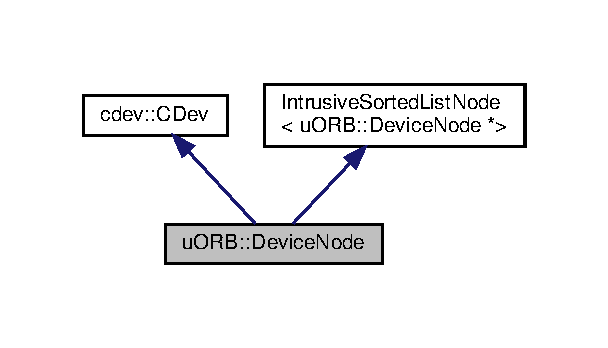
\includegraphics[width=292pt]{dc/d6b/classuORB_1_1DeviceNode__inherit__graph}
\end{center}
\end{figure}


Collaboration diagram for u\+O\+RB\+:\+:Device\+Node\+:\nopagebreak
\begin{figure}[H]
\begin{center}
\leavevmode
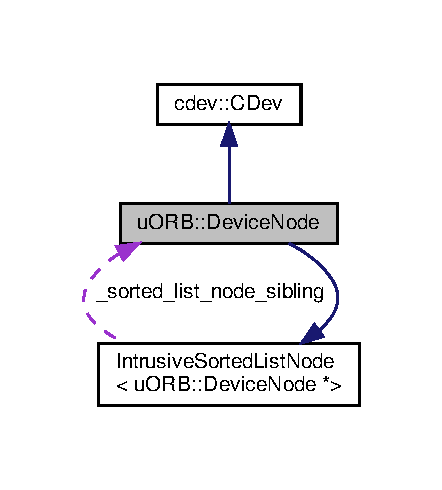
\includegraphics[width=212pt]{d7/dff/classuORB_1_1DeviceNode__coll__graph}
\end{center}
\end{figure}
\subsection*{Public Member Functions}
\begin{DoxyCompactItemize}
\item 
\mbox{\Hypertarget{classuORB_1_1DeviceNode_a34467219311e0a68acf87dd4f6cbdb5e}\label{classuORB_1_1DeviceNode_a34467219311e0a68acf87dd4f6cbdb5e}} 
{\bfseries Device\+Node} (const struct \hyperlink{structorb__metadata}{orb\+\_\+metadata} $\ast$meta, const uint8\+\_\+t instance, const char $\ast$path, uint8\+\_\+t queue\+\_\+size=1)
\item 
\mbox{\Hypertarget{classuORB_1_1DeviceNode_aacdd104881aaad56bb52cee63b972c3d}\label{classuORB_1_1DeviceNode_aacdd104881aaad56bb52cee63b972c3d}} 
{\bfseries Device\+Node} (const \hyperlink{classuORB_1_1DeviceNode}{Device\+Node} \&)=delete
\item 
\mbox{\Hypertarget{classuORB_1_1DeviceNode_a2819b13a6d7b7423f1bb61e01942cf4e}\label{classuORB_1_1DeviceNode_a2819b13a6d7b7423f1bb61e01942cf4e}} 
\hyperlink{classuORB_1_1DeviceNode}{Device\+Node} \& {\bfseries operator=} (const \hyperlink{classuORB_1_1DeviceNode}{Device\+Node} \&)=delete
\item 
\mbox{\Hypertarget{classuORB_1_1DeviceNode_abd5682d5d05a2dc8c31a4eb8190977f2}\label{classuORB_1_1DeviceNode_abd5682d5d05a2dc8c31a4eb8190977f2}} 
{\bfseries Device\+Node} (\hyperlink{classuORB_1_1DeviceNode}{Device\+Node} \&\&)=delete
\item 
\mbox{\Hypertarget{classuORB_1_1DeviceNode_aa7778a6a4195acf63d643b3cad431601}\label{classuORB_1_1DeviceNode_aa7778a6a4195acf63d643b3cad431601}} 
\hyperlink{classuORB_1_1DeviceNode}{Device\+Node} \& {\bfseries operator=} (\hyperlink{classuORB_1_1DeviceNode}{Device\+Node} \&\&)=delete
\item 
\mbox{\Hypertarget{classuORB_1_1DeviceNode_ae1bd88ecf550076f7c7f791b9be2af13}\label{classuORB_1_1DeviceNode_ae1bd88ecf550076f7c7f791b9be2af13}} 
bool {\bfseries operator$<$=} (const \hyperlink{classuORB_1_1DeviceNode}{Device\+Node} \&rhs) const
\item 
int \hyperlink{classuORB_1_1DeviceNode_ae7f3782c9876a17b4aa6949440655f1f}{open} (file $\ast$filp) override
\item 
int \hyperlink{classuORB_1_1DeviceNode_a80ebf695636c701d3378525b6d0e4148}{close} (file $\ast$filp) override
\item 
ssize\+\_\+t \hyperlink{classuORB_1_1DeviceNode_ada5db18aae221ae76e023651cbf9461c}{read} (file $\ast$filp, char $\ast$buffer, size\+\_\+t buflen) override
\item 
ssize\+\_\+t \hyperlink{classuORB_1_1DeviceNode_ab58b8b4b6cac9fd8aa4d90a85e044c78}{write} (file $\ast$filp, const char $\ast$buffer, size\+\_\+t buflen) override
\item 
int \hyperlink{classuORB_1_1DeviceNode_acad1520dfb19e9449546dad7a4129c26}{ioctl} (file $\ast$filp, int cmd, unsigned long arg) override
\item 
void \hyperlink{classuORB_1_1DeviceNode_abb03278ff4ddd2a50e0f2996e856f2cc}{add\+\_\+internal\+\_\+subscriber} ()
\item 
void \hyperlink{classuORB_1_1DeviceNode_ab4d0aa7c41ff0a8b2bf7b88fdc03d13d}{remove\+\_\+internal\+\_\+subscriber} ()
\item 
bool \hyperlink{classuORB_1_1DeviceNode_a16d1880bc99853428a8d8a240f24857b}{is\+\_\+advertised} () const
\item 
\mbox{\Hypertarget{classuORB_1_1DeviceNode_a5d9144fd43c624636a633d9dc288061a}\label{classuORB_1_1DeviceNode_a5d9144fd43c624636a633d9dc288061a}} 
void {\bfseries mark\+\_\+as\+\_\+advertised} ()
\item 
int \hyperlink{classuORB_1_1DeviceNode_aa4a59b86caeebbdf513dd60fcee1f5ba}{update\+\_\+queue\+\_\+size} (unsigned int queue\+\_\+size)
\item 
bool \hyperlink{classuORB_1_1DeviceNode_ad37197e0ca241eff70bd5aeeb4a811a2}{print\+\_\+statistics} (int max\+\_\+topic\+\_\+length)
\item 
\mbox{\Hypertarget{classuORB_1_1DeviceNode_a7877236ac1912c32c2ab6ae06899392d}\label{classuORB_1_1DeviceNode_a7877236ac1912c32c2ab6ae06899392d}} 
uint8\+\_\+t {\bfseries get\+\_\+queue\+\_\+size} () const
\item 
\mbox{\Hypertarget{classuORB_1_1DeviceNode_abccd5704db90417288e15fcfec5de633}\label{classuORB_1_1DeviceNode_abccd5704db90417288e15fcfec5de633}} 
int8\+\_\+t {\bfseries subscriber\+\_\+count} () const
\item 
\mbox{\Hypertarget{classuORB_1_1DeviceNode_a45adbc432af16d0f7dd5b8e0b4c0cc8b}\label{classuORB_1_1DeviceNode_a45adbc432af16d0f7dd5b8e0b4c0cc8b}} 
unsigned {\bfseries published\+\_\+message\+\_\+count} () const
\item 
\mbox{\Hypertarget{classuORB_1_1DeviceNode_a8de74e0e15d84cc83fb916c33fd87fba}\label{classuORB_1_1DeviceNode_a8de74e0e15d84cc83fb916c33fd87fba}} 
const \hyperlink{structorb__metadata}{orb\+\_\+metadata} $\ast$ {\bfseries get\+\_\+meta} () const
\item 
\mbox{\Hypertarget{classuORB_1_1DeviceNode_aa27dc606dff52f3c76fea72acb45230a}\label{classuORB_1_1DeviceNode_aa27dc606dff52f3c76fea72acb45230a}} 
\hyperlink{uORB_8h_a96af5434ec1acdf24287bd7851b0413f}{O\+R\+B\+\_\+\+ID} {\bfseries id} () const
\item 
\mbox{\Hypertarget{classuORB_1_1DeviceNode_aa99462996e1d4f1fc66bd3ca4dd5a3c0}\label{classuORB_1_1DeviceNode_aa99462996e1d4f1fc66bd3ca4dd5a3c0}} 
const char $\ast$ {\bfseries get\+\_\+name} () const
\item 
\mbox{\Hypertarget{classuORB_1_1DeviceNode_aa60643d933d54020c5b9201470b8e3c6}\label{classuORB_1_1DeviceNode_aa60643d933d54020c5b9201470b8e3c6}} 
uint8\+\_\+t {\bfseries get\+\_\+instance} () const
\item 
bool \hyperlink{classuORB_1_1DeviceNode_a89d9a792e1e38e04c65baba20f29d780}{copy} (void $\ast$dst, unsigned \&generation)
\item 
\mbox{\Hypertarget{classuORB_1_1DeviceNode_a402819fd9ba1c33e39389a47406b5ff7}\label{classuORB_1_1DeviceNode_a402819fd9ba1c33e39389a47406b5ff7}} 
bool {\bfseries register\+\_\+callback} (\hyperlink{classuORB_1_1SubscriptionCallback}{Subscription\+Callback} $\ast$callback\+\_\+sub)
\item 
\mbox{\Hypertarget{classuORB_1_1DeviceNode_aaaafc67863a203c52647a8dab4f48f2e}\label{classuORB_1_1DeviceNode_aaaafc67863a203c52647a8dab4f48f2e}} 
void {\bfseries unregister\+\_\+callback} (\hyperlink{classuORB_1_1SubscriptionCallback}{Subscription\+Callback} $\ast$callback\+\_\+sub)
\end{DoxyCompactItemize}
\subsection*{Static Public Member Functions}
\begin{DoxyCompactItemize}
\item 
static ssize\+\_\+t \hyperlink{classuORB_1_1DeviceNode_ae715517a1f3a2f361e37d061b59a4560}{publish} (const \hyperlink{structorb__metadata}{orb\+\_\+metadata} $\ast$meta, \hyperlink{uORB_8h_a8d0cfa5f9ea6427a37057d6cea6dd990}{orb\+\_\+advert\+\_\+t} handle, const void $\ast$data)
\item 
\mbox{\Hypertarget{classuORB_1_1DeviceNode_a07672cd375d8067080b76b8773659289}\label{classuORB_1_1DeviceNode_a07672cd375d8067080b76b8773659289}} 
static int {\bfseries unadvertise} (\hyperlink{uORB_8h_a8d0cfa5f9ea6427a37057d6cea6dd990}{orb\+\_\+advert\+\_\+t} handle)
\end{DoxyCompactItemize}
\subsection*{Protected Member Functions}
\begin{DoxyCompactItemize}
\item 
pollevent\+\_\+t \hyperlink{classuORB_1_1DeviceNode_a3ac7d5c93e5fd480cd623fd421afa060}{poll\+\_\+state} (file $\ast$filp) override
\item 
void \hyperlink{classuORB_1_1DeviceNode_a77061c03defdcb3eedfc9cdc8b38c003}{poll\+\_\+notify\+\_\+one} (struct pollfd $\ast$fds, pollevent\+\_\+t events) override
\end{DoxyCompactItemize}
\subsection*{Additional Inherited Members}


\subsection{Detailed Description}
Per-\/object device instance. 

Definition at line 58 of file u\+O\+R\+B\+Device\+Node.\+hpp.



\subsection{Member Function Documentation}
\mbox{\Hypertarget{classuORB_1_1DeviceNode_abb03278ff4ddd2a50e0f2996e856f2cc}\label{classuORB_1_1DeviceNode_abb03278ff4ddd2a50e0f2996e856f2cc}} 
\index{u\+O\+R\+B\+::\+Device\+Node@{u\+O\+R\+B\+::\+Device\+Node}!add\+\_\+internal\+\_\+subscriber@{add\+\_\+internal\+\_\+subscriber}}
\index{add\+\_\+internal\+\_\+subscriber@{add\+\_\+internal\+\_\+subscriber}!u\+O\+R\+B\+::\+Device\+Node@{u\+O\+R\+B\+::\+Device\+Node}}
\subsubsection{\texorpdfstring{add\+\_\+internal\+\_\+subscriber()}{add\_internal\_subscriber()}}
{\footnotesize\ttfamily void u\+O\+R\+B\+::\+Device\+Node\+::add\+\_\+internal\+\_\+subscriber (\begin{DoxyParamCaption}{ }\end{DoxyParamCaption})}

Add the subscriber to the node\textquotesingle{}s list of subscriber. If there is remote proxy to which this subscription needs to be sent, it will done via \hyperlink{classuORBCommunicator_1_1IChannel}{u\+O\+R\+B\+Communicator\+::\+I\+Channel} interface. 
\begin{DoxyParams}{Parameters}
{\em sd} & the subscriber to be added. \\
\hline
\end{DoxyParams}


Definition at line 408 of file u\+O\+R\+B\+Device\+Node.\+cpp.


\begin{DoxyCode}
409 \{
410     \hyperlink{classcdev_1_1CDev_ae676cccee31dd393ab681414a146d868}{lock}();
411     \_subscriber\_count++;
412 
413 \textcolor{preprocessor}{#ifdef ORB\_COMMUNICATOR}
414     \hyperlink{classuORBCommunicator_1_1IChannel}{uORBCommunicator::IChannel} *ch = 
      \hyperlink{classuORB_1_1Manager_a9d829b3ea49d16d03c2fa37ef2bb24a5}{uORB::Manager::get\_instance}()->get\_uorb\_communicator();
415 
416     \textcolor{keywordflow}{if} (ch != \textcolor{keyword}{nullptr} && \_subscriber\_count > 0) \{
417         \hyperlink{classcdev_1_1CDev_af65273e0578b277deea057dc7d558e9d}{unlock}(); \textcolor{comment}{//make sure we cannot deadlock if add\_subscription calls back into DeviceNode}
418         ch->\hyperlink{classuORBCommunicator_1_1IChannel_a2fdcab300f1c9ccf8c43858493ca9358}{add\_subscription}(\_meta->\hyperlink{structorb__metadata_a54d1751f24aa0c1f24934c6712811e58}{o\_name}, 1);
419 
420     \} \textcolor{keywordflow}{else}
421 \textcolor{preprocessor}{#endif }\textcolor{comment}{/* ORB\_COMMUNICATOR */}\textcolor{preprocessor}{}
422 
423     \{
424         \hyperlink{classcdev_1_1CDev_af65273e0578b277deea057dc7d558e9d}{unlock}();
425     \}
426 \}
\end{DoxyCode}
\mbox{\Hypertarget{classuORB_1_1DeviceNode_a80ebf695636c701d3378525b6d0e4148}\label{classuORB_1_1DeviceNode_a80ebf695636c701d3378525b6d0e4148}} 
\index{u\+O\+R\+B\+::\+Device\+Node@{u\+O\+R\+B\+::\+Device\+Node}!close@{close}}
\index{close@{close}!u\+O\+R\+B\+::\+Device\+Node@{u\+O\+R\+B\+::\+Device\+Node}}
\subsubsection{\texorpdfstring{close()}{close()}}
{\footnotesize\ttfamily int u\+O\+R\+B\+::\+Device\+Node\+::close (\begin{DoxyParamCaption}\item[{file $\ast$}]{filp }\end{DoxyParamCaption})\hspace{0.3cm}{\ttfamily [override]}, {\ttfamily [virtual]}}

Method to close a subscriber for this topic. 

Reimplemented from \hyperlink{classcdev_1_1CDev_a9241755ab3abf102eea85dad1e3dc6c4}{cdev\+::\+C\+Dev}.



Definition at line 118 of file u\+O\+R\+B\+Device\+Node.\+cpp.


\begin{DoxyCode}
119 \{
120     \textcolor{keywordflow}{if} (filp->f\_oflags == O\_RDONLY) \{ \textcolor{comment}{/* subscriber */}
121         SubscriptionInterval *sd = filp\_to\_subscription(filp);
122         \textcolor{keyword}{delete} sd;
123     \}
124 
125     \textcolor{keywordflow}{return} CDev::close(filp);
126 \}
\end{DoxyCode}
\mbox{\Hypertarget{classuORB_1_1DeviceNode_a89d9a792e1e38e04c65baba20f29d780}\label{classuORB_1_1DeviceNode_a89d9a792e1e38e04c65baba20f29d780}} 
\index{u\+O\+R\+B\+::\+Device\+Node@{u\+O\+R\+B\+::\+Device\+Node}!copy@{copy}}
\index{copy@{copy}!u\+O\+R\+B\+::\+Device\+Node@{u\+O\+R\+B\+::\+Device\+Node}}
\subsubsection{\texorpdfstring{copy()}{copy()}}
{\footnotesize\ttfamily bool u\+O\+R\+B\+::\+Device\+Node\+::copy (\begin{DoxyParamCaption}\item[{void $\ast$}]{dst,  }\item[{unsigned \&}]{generation }\end{DoxyParamCaption})}

Copies data and the corresponding generation from a node to the buffer provided.


\begin{DoxyParams}{Parameters}
{\em dst} & The buffer into which the data is copied. \\
\hline
{\em generation} & The generation that was copied. \\
\hline
\end{DoxyParams}
\begin{DoxyReturn}{Returns}
bool Returns true if the data was copied. 
\end{DoxyReturn}


Definition at line 128 of file u\+O\+R\+B\+Device\+Node.\+cpp.


\begin{DoxyCode}
129 \{
130     \textcolor{keywordflow}{if} ((dst != \textcolor{keyword}{nullptr}) && (\_data != \textcolor{keyword}{nullptr})) \{
131         \textcolor{keywordflow}{if} (\_queue\_size == 1) \{
132             ATOMIC\_ENTER;
133             memcpy(dst, \_data, \_meta->\hyperlink{structorb__metadata_a400a86fe707613e881b620cde7888b74}{o\_size});
134             generation = \_generation.load();
135             ATOMIC\_LEAVE;
136             \textcolor{keywordflow}{return} \textcolor{keyword}{true};
137 
138         \} \textcolor{keywordflow}{else} \{
139             ATOMIC\_ENTER;
140             \textcolor{keyword}{const} \textcolor{keywordtype}{unsigned} current\_generation = \_generation.load();
141 
142             \textcolor{keywordflow}{if} (current\_generation > generation + \_queue\_size) \{
143                 \textcolor{comment}{// Reader is too far behind: some messages are lost}
144                 generation = current\_generation - \_queue\_size;
145             \}
146 
147             \textcolor{keywordflow}{if} ((current\_generation == generation) && (generation > 0)) \{
148                 \textcolor{comment}{/* The subscriber already read the latest message, but nothing new was published yet.}
149 \textcolor{comment}{                * Return the previous message}
150 \textcolor{comment}{                */}
151                 --generation;
152             \}
153 
154             memcpy(dst, \_data + (\_meta->\hyperlink{structorb__metadata_a400a86fe707613e881b620cde7888b74}{o\_size} * (generation % \_queue\_size)), \_meta->
      \hyperlink{structorb__metadata_a400a86fe707613e881b620cde7888b74}{o\_size});
155             ATOMIC\_LEAVE;
156 
157             \textcolor{keywordflow}{if} (generation < current\_generation) \{
158                 ++generation;
159             \}
160 
161             \textcolor{keywordflow}{return} \textcolor{keyword}{true};
162         \}
163     \}
164 
165     \textcolor{keywordflow}{return} \textcolor{keyword}{false};
166 \}
\end{DoxyCode}
\mbox{\Hypertarget{classuORB_1_1DeviceNode_acad1520dfb19e9449546dad7a4129c26}\label{classuORB_1_1DeviceNode_acad1520dfb19e9449546dad7a4129c26}} 
\index{u\+O\+R\+B\+::\+Device\+Node@{u\+O\+R\+B\+::\+Device\+Node}!ioctl@{ioctl}}
\index{ioctl@{ioctl}!u\+O\+R\+B\+::\+Device\+Node@{u\+O\+R\+B\+::\+Device\+Node}}
\subsubsection{\texorpdfstring{ioctl()}{ioctl()}}
{\footnotesize\ttfamily int u\+O\+R\+B\+::\+Device\+Node\+::ioctl (\begin{DoxyParamCaption}\item[{file $\ast$}]{filp,  }\item[{int}]{cmd,  }\item[{unsigned long}]{arg }\end{DoxyParamCaption})\hspace{0.3cm}{\ttfamily [override]}, {\ttfamily [virtual]}}

I\+O\+C\+TL control for the subscriber. 

Reimplemented from \hyperlink{classcdev_1_1CDev_a87eb4d4b92a501de458736e8d24eec40}{cdev\+::\+C\+Dev}.



Definition at line 234 of file u\+O\+R\+B\+Device\+Node.\+cpp.


\begin{DoxyCode}
235 \{
236     \textcolor{keywordflow}{switch} (cmd) \{
237     \textcolor{keywordflow}{case} \hyperlink{drv__orb__dev_8h_a60e19540d21f9a44e9157804121957f8}{ORBIOCUPDATED}: \{
238             ATOMIC\_ENTER;
239             *(\textcolor{keywordtype}{bool} *)arg = filp\_to\_subscription(filp)->\hyperlink{classuORB_1_1SubscriptionInterval_aa1c12b83d65604e306b919a2c224e32e}{updated}();
240             ATOMIC\_LEAVE;
241             \textcolor{keywordflow}{return} 0;
242         \}
243 
244     \textcolor{keywordflow}{case} \hyperlink{drv__orb__dev_8h_a815da46533c3937c84c1496218659d0b}{ORBIOCSETINTERVAL}:
245         filp\_to\_subscription(filp)->\hyperlink{classuORB_1_1SubscriptionInterval_a53018b44bb431a80d47ac95327990b2a}{set\_interval\_us}(arg);
246         \textcolor{keywordflow}{return} 0;
247 
248     \textcolor{keywordflow}{case} \hyperlink{drv__orb__dev_8h_a0ba7c1d8b06e6930ed9589dbebbc775a}{ORBIOCGADVERTISER}:
249         *(uintptr\_t *)arg = (uintptr\_t)\textcolor{keyword}{this};
250         \textcolor{keywordflow}{return} 0;
251 
252     \textcolor{keywordflow}{case} \hyperlink{drv__orb__dev_8h_a4835f9286d5aac7a6b5e0a01661cbee7}{ORBIOCSETQUEUESIZE}: \{
253             \hyperlink{classcdev_1_1CDev_ae676cccee31dd393ab681414a146d868}{lock}();
254             \textcolor{keywordtype}{int} ret = \hyperlink{classuORB_1_1DeviceNode_aa4a59b86caeebbdf513dd60fcee1f5ba}{update\_queue\_size}(arg);
255             \hyperlink{classcdev_1_1CDev_af65273e0578b277deea057dc7d558e9d}{unlock}();
256             \textcolor{keywordflow}{return} ret;
257         \}
258 
259     \textcolor{keywordflow}{case} \hyperlink{drv__orb__dev_8h_acdbdb0d6f9b8600498ffa2599dca742d}{ORBIOCGETINTERVAL}:
260         *(\textcolor{keywordtype}{unsigned} *)arg = filp\_to\_subscription(filp)->get\_interval\_us();
261         \textcolor{keywordflow}{return} 0;
262 
263     \textcolor{keywordflow}{case} \hyperlink{drv__orb__dev_8h_a00f4a4fca062412c74b581a041c43c7a}{ORBIOCISADVERTISED}:
264         *(\textcolor{keywordtype}{unsigned} \textcolor{keywordtype}{long} *)arg = \_advertised;
265 
266         \textcolor{keywordflow}{return} 0;
267 
268     \textcolor{keywordflow}{default}:
269         \textcolor{comment}{/* give it to the superclass */}
270         \textcolor{keywordflow}{return} CDev::ioctl(filp, cmd, arg);
271     \}
272 \}
\end{DoxyCode}
\mbox{\Hypertarget{classuORB_1_1DeviceNode_a16d1880bc99853428a8d8a240f24857b}\label{classuORB_1_1DeviceNode_a16d1880bc99853428a8d8a240f24857b}} 
\index{u\+O\+R\+B\+::\+Device\+Node@{u\+O\+R\+B\+::\+Device\+Node}!is\+\_\+advertised@{is\+\_\+advertised}}
\index{is\+\_\+advertised@{is\+\_\+advertised}!u\+O\+R\+B\+::\+Device\+Node@{u\+O\+R\+B\+::\+Device\+Node}}
\subsubsection{\texorpdfstring{is\+\_\+advertised()}{is\_advertised()}}
{\footnotesize\ttfamily bool u\+O\+R\+B\+::\+Device\+Node\+::is\+\_\+advertised (\begin{DoxyParamCaption}{ }\end{DoxyParamCaption}) const\hspace{0.3cm}{\ttfamily [inline]}}

Return true if this topic has been advertised.

This is used in the case of multi\+\_\+pub/sub to check if it\textquotesingle{}s valid to advertise and publish to this node or if another node should be tried. 

Definition at line 169 of file u\+O\+R\+B\+Device\+Node.\+hpp.


\begin{DoxyCode}
169 \{ \textcolor{keywordflow}{return} \_advertised; \}
\end{DoxyCode}
\mbox{\Hypertarget{classuORB_1_1DeviceNode_ae7f3782c9876a17b4aa6949440655f1f}\label{classuORB_1_1DeviceNode_ae7f3782c9876a17b4aa6949440655f1f}} 
\index{u\+O\+R\+B\+::\+Device\+Node@{u\+O\+R\+B\+::\+Device\+Node}!open@{open}}
\index{open@{open}!u\+O\+R\+B\+::\+Device\+Node@{u\+O\+R\+B\+::\+Device\+Node}}
\subsubsection{\texorpdfstring{open()}{open()}}
{\footnotesize\ttfamily int u\+O\+R\+B\+::\+Device\+Node\+::open (\begin{DoxyParamCaption}\item[{file $\ast$}]{filp }\end{DoxyParamCaption})\hspace{0.3cm}{\ttfamily [override]}, {\ttfamily [virtual]}}

Method to create a subscriber instance and return the struct pointing to the subscriber as a file pointer. 

Reimplemented from \hyperlink{classcdev_1_1CDev_ac04b7ee91373c86545107e3467ba54c1}{cdev\+::\+C\+Dev}.



Definition at line 75 of file u\+O\+R\+B\+Device\+Node.\+cpp.


\begin{DoxyCode}
76 \{
77     \textcolor{comment}{/* is this a publisher? */}
78     \textcolor{keywordflow}{if} (filp->f\_oflags == O\_WRONLY) \{
79 
80         \hyperlink{classcdev_1_1CDev_ae676cccee31dd393ab681414a146d868}{lock}();
81         mark\_as\_advertised();
82         \hyperlink{classcdev_1_1CDev_af65273e0578b277deea057dc7d558e9d}{unlock}();
83 
84         \textcolor{comment}{/* now complete the open */}
85         \textcolor{keywordflow}{return} CDev::open(filp);
86     \}
87 
88     \textcolor{comment}{/* is this a new subscriber? */}
89     \textcolor{keywordflow}{if} (filp->f\_oflags == O\_RDONLY) \{
90 
91         \textcolor{comment}{/* allocate subscriber data */}
92         SubscriptionInterval *sd = \textcolor{keyword}{new} SubscriptionInterval(\_meta, 0, \_instance);
93 
94         \textcolor{keywordflow}{if} (\textcolor{keyword}{nullptr} == sd) \{
95             \textcolor{keywordflow}{return} -ENOMEM;
96         \}
97 
98         filp->f\_priv = (\textcolor{keywordtype}{void} *)sd;
99 
100         \textcolor{keywordtype}{int} ret = CDev::open(filp);
101 
102         \textcolor{keywordflow}{if} (ret != 0) \{
103             \textcolor{comment}{//PX4\_ERR("CDev::open failed");}
104             \textcolor{keyword}{delete} sd;
105         \}
106 
107         \textcolor{keywordflow}{return} ret;
108     \}
109 
110     \textcolor{keywordflow}{if} (filp->f\_oflags == 0) \{
111         \textcolor{keywordflow}{return} CDev::open(filp);
112     \}
113 
114     \textcolor{comment}{/* can only be pub or sub, not both */}
115     \textcolor{keywordflow}{return} -EINVAL;
116 \}
\end{DoxyCode}
\mbox{\Hypertarget{classuORB_1_1DeviceNode_a77061c03defdcb3eedfc9cdc8b38c003}\label{classuORB_1_1DeviceNode_a77061c03defdcb3eedfc9cdc8b38c003}} 
\index{u\+O\+R\+B\+::\+Device\+Node@{u\+O\+R\+B\+::\+Device\+Node}!poll\+\_\+notify\+\_\+one@{poll\+\_\+notify\+\_\+one}}
\index{poll\+\_\+notify\+\_\+one@{poll\+\_\+notify\+\_\+one}!u\+O\+R\+B\+::\+Device\+Node@{u\+O\+R\+B\+::\+Device\+Node}}
\subsubsection{\texorpdfstring{poll\+\_\+notify\+\_\+one()}{poll\_notify\_one()}}
{\footnotesize\ttfamily void u\+O\+R\+B\+::\+Device\+Node\+::poll\+\_\+notify\+\_\+one (\begin{DoxyParamCaption}\item[{struct pollfd $\ast$}]{fds,  }\item[{pollevent\+\_\+t}]{events }\end{DoxyParamCaption})\hspace{0.3cm}{\ttfamily [override]}, {\ttfamily [protected]}, {\ttfamily [virtual]}}

Internal implementation of poll\+\_\+notify.


\begin{DoxyParams}{Parameters}
{\em fds} & A poll waiter to notify. \\
\hline
{\em events} & The event(s) to send to the waiter. \\
\hline
\end{DoxyParams}


Reimplemented from \hyperlink{classcdev_1_1CDev_ada35d652d0f6d7257fffe4ead0fbb6dd}{cdev\+::\+C\+Dev}.



Definition at line 377 of file u\+O\+R\+B\+Device\+Node.\+cpp.


\begin{DoxyCode}
378 \{
379     \textcolor{comment}{// If the topic looks updated to the subscriber, go ahead and notify them.}
380     \textcolor{keywordflow}{if} (filp\_to\_subscription((file *)fds->priv)->\hyperlink{classuORB_1_1SubscriptionInterval_aa1c12b83d65604e306b919a2c224e32e}{updated}()) \{
381         CDev::poll\_notify\_one(fds, events);
382     \}
383 \}
\end{DoxyCode}
\mbox{\Hypertarget{classuORB_1_1DeviceNode_a3ac7d5c93e5fd480cd623fd421afa060}\label{classuORB_1_1DeviceNode_a3ac7d5c93e5fd480cd623fd421afa060}} 
\index{u\+O\+R\+B\+::\+Device\+Node@{u\+O\+R\+B\+::\+Device\+Node}!poll\+\_\+state@{poll\+\_\+state}}
\index{poll\+\_\+state@{poll\+\_\+state}!u\+O\+R\+B\+::\+Device\+Node@{u\+O\+R\+B\+::\+Device\+Node}}
\subsubsection{\texorpdfstring{poll\+\_\+state()}{poll\_state()}}
{\footnotesize\ttfamily pollevent\+\_\+t u\+O\+R\+B\+::\+Device\+Node\+::poll\+\_\+state (\begin{DoxyParamCaption}\item[{file $\ast$}]{filep }\end{DoxyParamCaption})\hspace{0.3cm}{\ttfamily [override]}, {\ttfamily [protected]}, {\ttfamily [virtual]}}

Check the current state of the device for poll events from the perspective of the file.

This function is called by the default \hyperlink{classcdev_1_1CDev_a219a565bb1842c62e0f45a7eeaaec0d3}{poll()} implementation when a poll is set up to determine whether the poll should return immediately.

The default implementation returns no events.


\begin{DoxyParams}{Parameters}
{\em filep} & The file that\textquotesingle{}s interested. \\
\hline
\end{DoxyParams}
\begin{DoxyReturn}{Returns}
The current set of poll events. 
\end{DoxyReturn}


Reimplemented from \hyperlink{classcdev_1_1CDev_abf40a822665b0889584268e8a4dfbef2}{cdev\+::\+C\+Dev}.



Definition at line 371 of file u\+O\+R\+B\+Device\+Node.\+cpp.


\begin{DoxyCode}
372 \{
373     \textcolor{comment}{// If the topic appears updated to the subscriber, say so.}
374     \textcolor{keywordflow}{return} filp\_to\_subscription(filp)->\hyperlink{classuORB_1_1SubscriptionInterval_aa1c12b83d65604e306b919a2c224e32e}{updated}() ? POLLIN : 0;
375 \}
\end{DoxyCode}
\mbox{\Hypertarget{classuORB_1_1DeviceNode_ad37197e0ca241eff70bd5aeeb4a811a2}\label{classuORB_1_1DeviceNode_ad37197e0ca241eff70bd5aeeb4a811a2}} 
\index{u\+O\+R\+B\+::\+Device\+Node@{u\+O\+R\+B\+::\+Device\+Node}!print\+\_\+statistics@{print\+\_\+statistics}}
\index{print\+\_\+statistics@{print\+\_\+statistics}!u\+O\+R\+B\+::\+Device\+Node@{u\+O\+R\+B\+::\+Device\+Node}}
\subsubsection{\texorpdfstring{print\+\_\+statistics()}{print\_statistics()}}
{\footnotesize\ttfamily bool u\+O\+R\+B\+::\+Device\+Node\+::print\+\_\+statistics (\begin{DoxyParamCaption}\item[{int}]{max\+\_\+topic\+\_\+length }\end{DoxyParamCaption})}

Print statistics 
\begin{DoxyParams}{Parameters}
{\em max\+\_\+topic\+\_\+length} & max topic name length for printing \\
\hline
\end{DoxyParams}
\begin{DoxyReturn}{Returns}
true if printed something, false otherwise 
\end{DoxyReturn}


Definition at line 385 of file u\+O\+R\+B\+Device\+Node.\+cpp.


\begin{DoxyCode}
386 \{
387     \textcolor{keywordflow}{if} (!\_advertised) \{
388         \textcolor{keywordflow}{return} \textcolor{keyword}{false};
389     \}
390 
391     \hyperlink{classcdev_1_1CDev_ae676cccee31dd393ab681414a146d868}{lock}();
392 
393     \textcolor{keyword}{const} uint8\_t instance = get\_instance();
394     \textcolor{keyword}{const} int8\_t sub\_count = subscriber\_count();
395     \textcolor{keyword}{const} uint8\_t queue\_size = get\_queue\_size();
396 
397     \hyperlink{classcdev_1_1CDev_af65273e0578b277deea057dc7d558e9d}{unlock}();
398 
399     printf(\textcolor{stringliteral}{"%2i %s %2i %4i %2i %4i %s\(\backslash\)n"}, max\_topic\_length, get\_meta()->o\_name, (\textcolor{keywordtype}{int})instance, (\textcolor{keywordtype}{int})
      sub\_count, \(\backslash\)
400              queue\_size, get\_meta()->o\_size, \hyperlink{classcdev_1_1CDev_a0bc1072e967a90dfac04a1227f200f6f}{get\_devname}());
401 
402     \textcolor{comment}{//PX4\_INFO\_RAW("%-*s %2i %4i %2i %4i %s\(\backslash\)n", max\_topic\_length, get\_meta()->o\_name, (int)instance,
       (int)sub\_count,}
403              \textcolor{comment}{//queue\_size, get\_meta()->o\_size, get\_devname());}
404 
405     \textcolor{keywordflow}{return} \textcolor{keyword}{true};
406 \}
\end{DoxyCode}
\mbox{\Hypertarget{classuORB_1_1DeviceNode_ae715517a1f3a2f361e37d061b59a4560}\label{classuORB_1_1DeviceNode_ae715517a1f3a2f361e37d061b59a4560}} 
\index{u\+O\+R\+B\+::\+Device\+Node@{u\+O\+R\+B\+::\+Device\+Node}!publish@{publish}}
\index{publish@{publish}!u\+O\+R\+B\+::\+Device\+Node@{u\+O\+R\+B\+::\+Device\+Node}}
\subsubsection{\texorpdfstring{publish()}{publish()}}
{\footnotesize\ttfamily ssize\+\_\+t u\+O\+R\+B\+::\+Device\+Node\+::publish (\begin{DoxyParamCaption}\item[{const \hyperlink{structorb__metadata}{orb\+\_\+metadata} $\ast$}]{meta,  }\item[{\hyperlink{uORB_8h_a8d0cfa5f9ea6427a37057d6cea6dd990}{orb\+\_\+advert\+\_\+t}}]{handle,  }\item[{const void $\ast$}]{data }\end{DoxyParamCaption})\hspace{0.3cm}{\ttfamily [static]}}

Method to publish a data to this node. 

Definition at line 274 of file u\+O\+R\+B\+Device\+Node.\+cpp.


\begin{DoxyCode}
275 \{
276     \hyperlink{classuORB_1_1DeviceNode}{uORB::DeviceNode} *devnode = (\hyperlink{classuORB_1_1DeviceNode}{uORB::DeviceNode} *)handle;
277     \textcolor{keywordtype}{int} ret;
278 
279     \textcolor{comment}{/* check if the device handle is initialized and data is valid */}
280     \textcolor{keywordflow}{if} ((devnode == \textcolor{keyword}{nullptr}) || (meta == \textcolor{keyword}{nullptr}) || (data == \textcolor{keyword}{nullptr})) \{
281         errno = EFAULT;
282         \textcolor{keywordflow}{return} -1;
283     \}
284 
285     \textcolor{comment}{/* check if the orb meta data matches the publication */}
286     \textcolor{keywordflow}{if} (devnode->\_meta != meta) \{
287         errno = EINVAL;
288         \textcolor{keywordflow}{return} -1;
289     \}
290 
291     \textcolor{comment}{/* call the devnode write method with no file pointer */}
292     ret = devnode->\hyperlink{classuORB_1_1DeviceNode_ab58b8b4b6cac9fd8aa4d90a85e044c78}{write}(\textcolor{keyword}{nullptr}, (\textcolor{keyword}{const} \textcolor{keywordtype}{char} *)data, meta->\hyperlink{structorb__metadata_a400a86fe707613e881b620cde7888b74}{o\_size});
293 
294     \textcolor{keywordflow}{if} (ret < 0) \{
295         errno = -ret;
296         \textcolor{keywordflow}{return} -1;
297     \}
298 
299     \textcolor{keywordflow}{if} (ret != (\textcolor{keywordtype}{int})meta->\hyperlink{structorb__metadata_a400a86fe707613e881b620cde7888b74}{o\_size}) \{
300         errno = EIO;
301         \textcolor{keywordflow}{return} -1;
302     \}
303 
304 \textcolor{preprocessor}{#ifdef ORB\_COMMUNICATOR}
305     \textcolor{comment}{/*}
306 \textcolor{comment}{     * if the write is successful, send the data over the Multi-ORB link}
307 \textcolor{comment}{     */}
308     \hyperlink{classuORBCommunicator_1_1IChannel}{uORBCommunicator::IChannel} *ch = 
      \hyperlink{classuORB_1_1Manager_a9d829b3ea49d16d03c2fa37ef2bb24a5}{uORB::Manager::get\_instance}()->get\_uorb\_communicator();
309 
310     \textcolor{keywordflow}{if} (ch != \textcolor{keyword}{nullptr}) \{
311         \textcolor{keywordflow}{if} (ch->\hyperlink{classuORBCommunicator_1_1IChannel_a3f4690d7b897f5f568cfed2c31d7b734}{send\_message}(meta->\hyperlink{structorb__metadata_a54d1751f24aa0c1f24934c6712811e58}{o\_name}, meta->\hyperlink{structorb__metadata_a400a86fe707613e881b620cde7888b74}{o\_size}, (uint8\_t *)data) != 0) \{
312             PX4\_ERR(\textcolor{stringliteral}{"Error Sending [%s] topic data over comm\_channel"}, meta->
      \hyperlink{structorb__metadata_a54d1751f24aa0c1f24934c6712811e58}{o\_name});
313             \textcolor{keywordflow}{return} -1;
314         \}
315     \}
316 
317 \textcolor{preprocessor}{#endif }\textcolor{comment}{/* ORB\_COMMUNICATOR */}\textcolor{preprocessor}{}
318 
319     \textcolor{keywordflow}{return} 0;
320 \}
\end{DoxyCode}
\mbox{\Hypertarget{classuORB_1_1DeviceNode_ada5db18aae221ae76e023651cbf9461c}\label{classuORB_1_1DeviceNode_ada5db18aae221ae76e023651cbf9461c}} 
\index{u\+O\+R\+B\+::\+Device\+Node@{u\+O\+R\+B\+::\+Device\+Node}!read@{read}}
\index{read@{read}!u\+O\+R\+B\+::\+Device\+Node@{u\+O\+R\+B\+::\+Device\+Node}}
\subsubsection{\texorpdfstring{read()}{read()}}
{\footnotesize\ttfamily ssize\+\_\+t u\+O\+R\+B\+::\+Device\+Node\+::read (\begin{DoxyParamCaption}\item[{file $\ast$}]{filp,  }\item[{char $\ast$}]{buffer,  }\item[{size\+\_\+t}]{buflen }\end{DoxyParamCaption})\hspace{0.3cm}{\ttfamily [override]}, {\ttfamily [virtual]}}

reads data from a subscriber node to the buffer provided. 
\begin{DoxyParams}{Parameters}
{\em filp} & The subscriber from which the data needs to be read from. \\
\hline
{\em buffer} & The buffer into which the data is read into. \\
\hline
{\em buflen} & the length of the buffer \\
\hline
\end{DoxyParams}
\begin{DoxyReturn}{Returns}
ssize\+\_\+t the number of bytes read. 
\end{DoxyReturn}


Reimplemented from \hyperlink{classcdev_1_1CDev_a1b0db49c478b621333aff6bb3321d057}{cdev\+::\+C\+Dev}.



Definition at line 168 of file u\+O\+R\+B\+Device\+Node.\+cpp.


\begin{DoxyCode}
169 \{
170     \textcolor{comment}{/* if the caller's buffer is the wrong size, that's an error */}
171     \textcolor{keywordflow}{if} (buflen != \_meta->\hyperlink{structorb__metadata_a400a86fe707613e881b620cde7888b74}{o\_size}) \{
172         \textcolor{keywordflow}{return} -EIO;
173     \}
174 
175     \textcolor{keywordflow}{return} filp\_to\_subscription(filp)->\hyperlink{classuORB_1_1SubscriptionInterval_a25125ed09772665d3b4b4e6978fb3e1c}{copy}(buffer) ? \_meta->\hyperlink{structorb__metadata_a400a86fe707613e881b620cde7888b74}{o\_size} : 0;
176 \}
\end{DoxyCode}
\mbox{\Hypertarget{classuORB_1_1DeviceNode_ab4d0aa7c41ff0a8b2bf7b88fdc03d13d}\label{classuORB_1_1DeviceNode_ab4d0aa7c41ff0a8b2bf7b88fdc03d13d}} 
\index{u\+O\+R\+B\+::\+Device\+Node@{u\+O\+R\+B\+::\+Device\+Node}!remove\+\_\+internal\+\_\+subscriber@{remove\+\_\+internal\+\_\+subscriber}}
\index{remove\+\_\+internal\+\_\+subscriber@{remove\+\_\+internal\+\_\+subscriber}!u\+O\+R\+B\+::\+Device\+Node@{u\+O\+R\+B\+::\+Device\+Node}}
\subsubsection{\texorpdfstring{remove\+\_\+internal\+\_\+subscriber()}{remove\_internal\_subscriber()}}
{\footnotesize\ttfamily void u\+O\+R\+B\+::\+Device\+Node\+::remove\+\_\+internal\+\_\+subscriber (\begin{DoxyParamCaption}{ }\end{DoxyParamCaption})}

Removes the subscriber from the list. Also notifies the remote if there a \hyperlink{classuORBCommunicator_1_1IChannel}{u\+O\+R\+B\+Communicator\+::\+I\+Channel} instance. 
\begin{DoxyParams}{Parameters}
{\em sd} & the Subscriber to be removed. \\
\hline
\end{DoxyParams}


Definition at line 428 of file u\+O\+R\+B\+Device\+Node.\+cpp.


\begin{DoxyCode}
429 \{
430     \hyperlink{classcdev_1_1CDev_ae676cccee31dd393ab681414a146d868}{lock}();
431     \_subscriber\_count--;
432 
433 \textcolor{preprocessor}{#ifdef ORB\_COMMUNICATOR}
434     \hyperlink{classuORBCommunicator_1_1IChannel}{uORBCommunicator::IChannel} *ch = 
      \hyperlink{classuORB_1_1Manager_a9d829b3ea49d16d03c2fa37ef2bb24a5}{uORB::Manager::get\_instance}()->get\_uorb\_communicator();
435 
436     \textcolor{keywordflow}{if} (ch != \textcolor{keyword}{nullptr} && \_subscriber\_count == 0) \{
437         \hyperlink{classcdev_1_1CDev_af65273e0578b277deea057dc7d558e9d}{unlock}(); \textcolor{comment}{//make sure we cannot deadlock if remove\_subscription calls back into DeviceNode}
438         ch->\hyperlink{classuORBCommunicator_1_1IChannel_a74420541552346f0367d802b5c61714a}{remove\_subscription}(\_meta->\hyperlink{structorb__metadata_a54d1751f24aa0c1f24934c6712811e58}{o\_name});
439 
440     \} \textcolor{keywordflow}{else}
441 \textcolor{preprocessor}{#endif }\textcolor{comment}{/* ORB\_COMMUNICATOR */}\textcolor{preprocessor}{}
442     \{
443         \hyperlink{classcdev_1_1CDev_af65273e0578b277deea057dc7d558e9d}{unlock}();
444     \}
445 \}
\end{DoxyCode}
\mbox{\Hypertarget{classuORB_1_1DeviceNode_aa4a59b86caeebbdf513dd60fcee1f5ba}\label{classuORB_1_1DeviceNode_aa4a59b86caeebbdf513dd60fcee1f5ba}} 
\index{u\+O\+R\+B\+::\+Device\+Node@{u\+O\+R\+B\+::\+Device\+Node}!update\+\_\+queue\+\_\+size@{update\+\_\+queue\+\_\+size}}
\index{update\+\_\+queue\+\_\+size@{update\+\_\+queue\+\_\+size}!u\+O\+R\+B\+::\+Device\+Node@{u\+O\+R\+B\+::\+Device\+Node}}
\subsubsection{\texorpdfstring{update\+\_\+queue\+\_\+size()}{update\_queue\_size()}}
{\footnotesize\ttfamily int u\+O\+R\+B\+::\+Device\+Node\+::update\+\_\+queue\+\_\+size (\begin{DoxyParamCaption}\item[{unsigned int}]{queue\+\_\+size }\end{DoxyParamCaption})}

Try to change the size of the queue. This can only be done as long as nobody published yet. This is the case, for example when orb\+\_\+subscribe was called before an orb\+\_\+advertise. The queue size can only be increased. 
\begin{DoxyParams}{Parameters}
{\em queue\+\_\+size} & new size of the queue \\
\hline
\end{DoxyParams}
\begin{DoxyReturn}{Returns}
P\+X4\+\_\+\+OK if queue size successfully set 
\end{DoxyReturn}


Definition at line 492 of file u\+O\+R\+B\+Device\+Node.\+cpp.


\begin{DoxyCode}
493 \{
494     \textcolor{keywordflow}{if} (\_queue\_size == queue\_size) \{
495         \textcolor{keywordflow}{return} 0;
496     \}
497 
498     \textcolor{comment}{//queue size is limited to 255 for the single reason that we use uint8 to store it}
499     \textcolor{keywordflow}{if} (\_data || \_queue\_size > queue\_size || queue\_size > 255) \{
500         \textcolor{keywordflow}{return} -1;
501     \}
502 
503     \_queue\_size = queue\_size;
504     \textcolor{keywordflow}{return} 0;
505 \}
\end{DoxyCode}
\mbox{\Hypertarget{classuORB_1_1DeviceNode_ab58b8b4b6cac9fd8aa4d90a85e044c78}\label{classuORB_1_1DeviceNode_ab58b8b4b6cac9fd8aa4d90a85e044c78}} 
\index{u\+O\+R\+B\+::\+Device\+Node@{u\+O\+R\+B\+::\+Device\+Node}!write@{write}}
\index{write@{write}!u\+O\+R\+B\+::\+Device\+Node@{u\+O\+R\+B\+::\+Device\+Node}}
\subsubsection{\texorpdfstring{write()}{write()}}
{\footnotesize\ttfamily ssize\+\_\+t u\+O\+R\+B\+::\+Device\+Node\+::write (\begin{DoxyParamCaption}\item[{file $\ast$}]{filp,  }\item[{const char $\ast$}]{buffer,  }\item[{size\+\_\+t}]{buflen }\end{DoxyParamCaption})\hspace{0.3cm}{\ttfamily [override]}, {\ttfamily [virtual]}}

writes the published data to the internal buffer to be read by subscribers later. 
\begin{DoxyParams}{Parameters}
{\em filp} & the subscriber; this is not used. \\
\hline
{\em buffer} & The buffer for the input data \\
\hline
{\em buflen} & the length of the buffer. \\
\hline
\end{DoxyParams}
\begin{DoxyReturn}{Returns}
ssize\+\_\+t The number of bytes that are written 
\end{DoxyReturn}


Reimplemented from \hyperlink{classcdev_1_1CDev_a54aff43049b22cea19f8cc31cb2a0fd0}{cdev\+::\+C\+Dev}.



Definition at line 178 of file u\+O\+R\+B\+Device\+Node.\+cpp.


\begin{DoxyCode}
179 \{
180     \textcolor{comment}{/*}
181 \textcolor{comment}{     * Writes are legal from interrupt context as long as the}
182 \textcolor{comment}{     * object has already been initialised from thread context.}
183 \textcolor{comment}{     *}
184 \textcolor{comment}{     * Writes outside interrupt context will allocate the object}
185 \textcolor{comment}{     * if it has not yet been allocated.}
186 \textcolor{comment}{     *}
187 \textcolor{comment}{     * Note that filp will usually be NULL.}
188 \textcolor{comment}{     */}
189     \textcolor{keywordflow}{if} (\textcolor{keyword}{nullptr} == \_data) \{
190 
191         \textcolor{keywordflow}{if} (!up\_interrupt\_context()) \{
192 
193             \hyperlink{classcdev_1_1CDev_ae676cccee31dd393ab681414a146d868}{lock}();
194 
195             \textcolor{comment}{/* re-check size */}
196             \textcolor{keywordflow}{if} (\textcolor{keyword}{nullptr} == \_data) \{
197                 \_data = \textcolor{keyword}{new} uint8\_t[\_meta->\hyperlink{structorb__metadata_a400a86fe707613e881b620cde7888b74}{o\_size} * \_queue\_size];
198             \}
199 
200             \hyperlink{classcdev_1_1CDev_af65273e0578b277deea057dc7d558e9d}{unlock}();
201         \}
202 
203         \textcolor{comment}{/* failed or could not allocate */}
204         \textcolor{keywordflow}{if} (\textcolor{keyword}{nullptr} == \_data) \{
205             \textcolor{keywordflow}{return} -ENOMEM;
206         \}
207     \}
208 
209     \textcolor{comment}{/* If write size does not match, that is an error */}
210     \textcolor{keywordflow}{if} (\_meta->\hyperlink{structorb__metadata_a400a86fe707613e881b620cde7888b74}{o\_size} != buflen) \{
211         \textcolor{keywordflow}{return} -EIO;
212     \}
213 
214     \textcolor{comment}{/* Perform an atomic copy. */}
215     ATOMIC\_ENTER;
216     \textcolor{comment}{/* wrap-around happens after ~49 days, assuming a publisher rate of 1 kHz */}
217     \textcolor{keywordtype}{unsigned} generation = \_generation.fetch\_add(1);
218 
219     memcpy(\_data + (\_meta->\hyperlink{structorb__metadata_a400a86fe707613e881b620cde7888b74}{o\_size} * (generation % \_queue\_size)), buffer, \_meta->
      \hyperlink{structorb__metadata_a400a86fe707613e881b620cde7888b74}{o\_size});
220 
221     \textcolor{comment}{// callbacks}
222     \textcolor{keywordflow}{for} (\textcolor{keyword}{auto} item : \_callbacks) \{
223         item->call();
224     \}
225 
226     ATOMIC\_LEAVE;
227 
228     \textcolor{comment}{/* notify any poll waiters */}
229     \hyperlink{classcdev_1_1CDev_aa23e0fac4d51f7b14db7a7e7dfa0ac06}{poll\_notify}(POLLIN);
230 
231     \textcolor{keywordflow}{return} \_meta->\hyperlink{structorb__metadata_a400a86fe707613e881b620cde7888b74}{o\_size};
232 \}
\end{DoxyCode}


The documentation for this class was generated from the following files\+:\begin{DoxyCompactItemize}
\item 
/home/andressanchez/\+Escritorio/\+G\+I\+T/project\+\_\+template/src/modules/u\+O\+R\+B/u\+O\+R\+B\+Device\+Node.\+hpp\item 
/home/andressanchez/\+Escritorio/\+G\+I\+T/project\+\_\+template/src/modules/u\+O\+R\+B/u\+O\+R\+B\+Device\+Node.\+cpp\end{DoxyCompactItemize}

\hypertarget{structhrt__call}{}\section{hrt\+\_\+call Struct Reference}
\label{structhrt__call}\index{hrt\+\_\+call@{hrt\+\_\+call}}


{\ttfamily \#include $<$drv\+\_\+hrt.\+h$>$}

\subsection*{Public Attributes}
\begin{DoxyCompactItemize}
\item 
\mbox{\Hypertarget{structhrt__call_a9e5f0257838253f2154864304a32ab02}\label{structhrt__call_a9e5f0257838253f2154864304a32ab02}} 
struct sq\+\_\+entry\+\_\+s {\bfseries link}
\item 
\mbox{\Hypertarget{structhrt__call_a6ceccf9f1cf61c19960af17834c17a84}\label{structhrt__call_a6ceccf9f1cf61c19960af17834c17a84}} 
\hyperlink{drv__hrt_8h_a9f8bbf0e883115e04a457a268533a87c}{hrt\+\_\+abstime} {\bfseries deadline}
\item 
\mbox{\Hypertarget{structhrt__call_a92d4cb2db34d9f449df684dea2f1faa8}\label{structhrt__call_a92d4cb2db34d9f449df684dea2f1faa8}} 
\hyperlink{drv__hrt_8h_a9f8bbf0e883115e04a457a268533a87c}{hrt\+\_\+abstime} {\bfseries period}
\item 
\mbox{\Hypertarget{structhrt__call_aad5880605fa741b171aa10456a959e3c}\label{structhrt__call_aad5880605fa741b171aa10456a959e3c}} 
\hyperlink{drv__hrt_8h_ac8f5a61245c186b72dbbd2466dcceea5}{hrt\+\_\+callout} {\bfseries callout}
\item 
\mbox{\Hypertarget{structhrt__call_afe59f717509a796f96993d472de718d0}\label{structhrt__call_afe59f717509a796f96993d472de718d0}} 
void $\ast$ {\bfseries arg}
\end{DoxyCompactItemize}


\subsection{Detailed Description}
Callout record. 

Definition at line 80 of file drv\+\_\+hrt.\+h.



The documentation for this struct was generated from the following file\+:\begin{DoxyCompactItemize}
\item 
/home/andressanchez/\+Escritorio/\+G\+I\+T/project\+\_\+template/src/drivers/\hyperlink{drv__hrt_8h}{drv\+\_\+hrt.\+h}\end{DoxyCompactItemize}

\hypertarget{classuORBCommunicator_1_1IChannel}{}\section{u\+O\+R\+B\+Communicator\+:\+:I\+Channel Class Reference}
\label{classuORBCommunicator_1_1IChannel}\index{u\+O\+R\+B\+Communicator\+::\+I\+Channel@{u\+O\+R\+B\+Communicator\+::\+I\+Channel}}


{\ttfamily \#include $<$u\+O\+R\+B\+Communicator.\+hpp$>$}

\subsection*{Public Member Functions}
\begin{DoxyCompactItemize}
\item 
virtual int16\+\_\+t \hyperlink{classuORBCommunicator_1_1IChannel_a77ca809a54e4d7a0137e89eeba22d17f}{topic\+\_\+advertised} (const char $\ast$message\+Name)=0
\begin{DoxyCompactList}\small\item\em Interface to notify the remote entity of a topic being advertised. \end{DoxyCompactList}\item 
virtual int16\+\_\+t \hyperlink{classuORBCommunicator_1_1IChannel_a2fdcab300f1c9ccf8c43858493ca9358}{add\+\_\+subscription} (const char $\ast$message\+Name, int32\+\_\+t msg\+Rate\+In\+Hz)=0
\begin{DoxyCompactList}\small\item\em Interface to notify the remote entity of a topic being unadvertised and is no longer publishing messages. \end{DoxyCompactList}\item 
virtual int16\+\_\+t \hyperlink{classuORBCommunicator_1_1IChannel_a74420541552346f0367d802b5c61714a}{remove\+\_\+subscription} (const char $\ast$message\+Name)=0
\begin{DoxyCompactList}\small\item\em Interface to notify the remote entity of removal of a subscription. \end{DoxyCompactList}\item 
virtual int16\+\_\+t \hyperlink{classuORBCommunicator_1_1IChannel_aba1c6e430848e447334c5be5c06e1d14}{register\+\_\+handler} (\hyperlink{classuORBCommunicator_1_1IChannelRxHandler}{u\+O\+R\+B\+Communicator\+::\+I\+Channel\+Rx\+Handler} $\ast$handler)=0
\item 
virtual int16\+\_\+t \hyperlink{classuORBCommunicator_1_1IChannel_a3f4690d7b897f5f568cfed2c31d7b734}{send\+\_\+message} (const char $\ast$message\+Name, int32\+\_\+t length, uint8\+\_\+t $\ast$data)=0
\begin{DoxyCompactList}\small\item\em Sends the data message over the communication link. \end{DoxyCompactList}\end{DoxyCompactItemize}


\subsection{Detailed Description}
Interface to enable remote subscriptions. The implementor of this interface shall manage the communication channel. It can be fast\+R\+PC or tcp or ip. 

Definition at line 51 of file u\+O\+R\+B\+Communicator.\+hpp.



\subsection{Member Function Documentation}
\mbox{\Hypertarget{classuORBCommunicator_1_1IChannel_a2fdcab300f1c9ccf8c43858493ca9358}\label{classuORBCommunicator_1_1IChannel_a2fdcab300f1c9ccf8c43858493ca9358}} 
\index{u\+O\+R\+B\+Communicator\+::\+I\+Channel@{u\+O\+R\+B\+Communicator\+::\+I\+Channel}!add\+\_\+subscription@{add\+\_\+subscription}}
\index{add\+\_\+subscription@{add\+\_\+subscription}!u\+O\+R\+B\+Communicator\+::\+I\+Channel@{u\+O\+R\+B\+Communicator\+::\+I\+Channel}}
\subsubsection{\texorpdfstring{add\+\_\+subscription()}{add\_subscription()}}
{\footnotesize\ttfamily virtual int16\+\_\+t u\+O\+R\+B\+Communicator\+::\+I\+Channel\+::add\+\_\+subscription (\begin{DoxyParamCaption}\item[{const char $\ast$}]{message\+Name,  }\item[{int32\+\_\+t}]{msg\+Rate\+In\+Hz }\end{DoxyParamCaption})\hspace{0.3cm}{\ttfamily [pure virtual]}}



Interface to notify the remote entity of a topic being unadvertised and is no longer publishing messages. 


\begin{DoxyParams}{Parameters}
{\em message\+Name} & This represents the u\+O\+RB message name(aka topic); This message name should be globally unique. \\
\hline
\end{DoxyParams}
\begin{DoxyReturn}{Returns}
0 = success; This means the messages is successfully sent to the receiver Note\+: This does not mean that the receiver as received it. otherwise = failure. Interface to notify the remote entity of interest of a subscription for a message.
\end{DoxyReturn}

\begin{DoxyParams}{Parameters}
{\em message\+Name} & This represents the u\+O\+RB message name; This message name should be globally unique. \\
\hline
{\em msg\+Rate} & The max rate at which the subscriber can accept the messages. \\
\hline
\end{DoxyParams}
\begin{DoxyReturn}{Returns}
0 = success; This means the messages is successfully sent to the receiver Note\+: This does not mean that the receiver as received it. otherwise = failure. 
\end{DoxyReturn}
\mbox{\Hypertarget{classuORBCommunicator_1_1IChannel_aba1c6e430848e447334c5be5c06e1d14}\label{classuORBCommunicator_1_1IChannel_aba1c6e430848e447334c5be5c06e1d14}} 
\index{u\+O\+R\+B\+Communicator\+::\+I\+Channel@{u\+O\+R\+B\+Communicator\+::\+I\+Channel}!register\+\_\+handler@{register\+\_\+handler}}
\index{register\+\_\+handler@{register\+\_\+handler}!u\+O\+R\+B\+Communicator\+::\+I\+Channel@{u\+O\+R\+B\+Communicator\+::\+I\+Channel}}
\subsubsection{\texorpdfstring{register\+\_\+handler()}{register\_handler()}}
{\footnotesize\ttfamily virtual int16\+\_\+t u\+O\+R\+B\+Communicator\+::\+I\+Channel\+::register\+\_\+handler (\begin{DoxyParamCaption}\item[{\hyperlink{classuORBCommunicator_1_1IChannelRxHandler}{u\+O\+R\+B\+Communicator\+::\+I\+Channel\+Rx\+Handler} $\ast$}]{handler }\end{DoxyParamCaption})\hspace{0.3cm}{\ttfamily [pure virtual]}}

Register Message Handler. This is internal for the \hyperlink{classuORBCommunicator_1_1IChannel}{I\+Channel} implementer$\ast$ \mbox{\Hypertarget{classuORBCommunicator_1_1IChannel_a74420541552346f0367d802b5c61714a}\label{classuORBCommunicator_1_1IChannel_a74420541552346f0367d802b5c61714a}} 
\index{u\+O\+R\+B\+Communicator\+::\+I\+Channel@{u\+O\+R\+B\+Communicator\+::\+I\+Channel}!remove\+\_\+subscription@{remove\+\_\+subscription}}
\index{remove\+\_\+subscription@{remove\+\_\+subscription}!u\+O\+R\+B\+Communicator\+::\+I\+Channel@{u\+O\+R\+B\+Communicator\+::\+I\+Channel}}
\subsubsection{\texorpdfstring{remove\+\_\+subscription()}{remove\_subscription()}}
{\footnotesize\ttfamily virtual int16\+\_\+t u\+O\+R\+B\+Communicator\+::\+I\+Channel\+::remove\+\_\+subscription (\begin{DoxyParamCaption}\item[{const char $\ast$}]{message\+Name }\end{DoxyParamCaption})\hspace{0.3cm}{\ttfamily [pure virtual]}}



Interface to notify the remote entity of removal of a subscription. 


\begin{DoxyParams}{Parameters}
{\em message\+Name} & This represents the u\+O\+RB message name; This message name should be globally unique. \\
\hline
\end{DoxyParams}
\begin{DoxyReturn}{Returns}
0 = success; This means the messages is successfully sent to the receiver Note\+: This does not necessarily mean that the receiver as received it. otherwise = failure. 
\end{DoxyReturn}
\mbox{\Hypertarget{classuORBCommunicator_1_1IChannel_a3f4690d7b897f5f568cfed2c31d7b734}\label{classuORBCommunicator_1_1IChannel_a3f4690d7b897f5f568cfed2c31d7b734}} 
\index{u\+O\+R\+B\+Communicator\+::\+I\+Channel@{u\+O\+R\+B\+Communicator\+::\+I\+Channel}!send\+\_\+message@{send\+\_\+message}}
\index{send\+\_\+message@{send\+\_\+message}!u\+O\+R\+B\+Communicator\+::\+I\+Channel@{u\+O\+R\+B\+Communicator\+::\+I\+Channel}}
\subsubsection{\texorpdfstring{send\+\_\+message()}{send\_message()}}
{\footnotesize\ttfamily virtual int16\+\_\+t u\+O\+R\+B\+Communicator\+::\+I\+Channel\+::send\+\_\+message (\begin{DoxyParamCaption}\item[{const char $\ast$}]{message\+Name,  }\item[{int32\+\_\+t}]{length,  }\item[{uint8\+\_\+t $\ast$}]{data }\end{DoxyParamCaption})\hspace{0.3cm}{\ttfamily [pure virtual]}}



Sends the data message over the communication link. 


\begin{DoxyParams}{Parameters}
{\em message\+Name} & This represents the u\+O\+RB message name; This message name should be globally unique. \\
\hline
{\em length} & The length of the data buffer to be sent. \\
\hline
{\em data} & The actual data to be sent. \\
\hline
\end{DoxyParams}
\begin{DoxyReturn}{Returns}
0 = success; This means the messages is successfully sent to the receiver Note\+: This does not mean that the receiver as received it. otherwise = failure. 
\end{DoxyReturn}
\mbox{\Hypertarget{classuORBCommunicator_1_1IChannel_a77ca809a54e4d7a0137e89eeba22d17f}\label{classuORBCommunicator_1_1IChannel_a77ca809a54e4d7a0137e89eeba22d17f}} 
\index{u\+O\+R\+B\+Communicator\+::\+I\+Channel@{u\+O\+R\+B\+Communicator\+::\+I\+Channel}!topic\+\_\+advertised@{topic\+\_\+advertised}}
\index{topic\+\_\+advertised@{topic\+\_\+advertised}!u\+O\+R\+B\+Communicator\+::\+I\+Channel@{u\+O\+R\+B\+Communicator\+::\+I\+Channel}}
\subsubsection{\texorpdfstring{topic\+\_\+advertised()}{topic\_advertised()}}
{\footnotesize\ttfamily virtual int16\+\_\+t u\+O\+R\+B\+Communicator\+::\+I\+Channel\+::topic\+\_\+advertised (\begin{DoxyParamCaption}\item[{const char $\ast$}]{message\+Name }\end{DoxyParamCaption})\hspace{0.3cm}{\ttfamily [pure virtual]}}



Interface to notify the remote entity of a topic being advertised. 


\begin{DoxyParams}{Parameters}
{\em message\+Name} & This represents the u\+O\+RB message name(aka topic); This message name should be globally unique. \\
\hline
\end{DoxyParams}
\begin{DoxyReturn}{Returns}
0 = success; This means the messages is successfully sent to the receiver Note\+: This does not mean that the receiver as received it. otherwise = failure. 
\end{DoxyReturn}


The documentation for this class was generated from the following file\+:\begin{DoxyCompactItemize}
\item 
/home/andressanchez/\+Escritorio/\+G\+I\+T/project\+\_\+template/src/modules/u\+O\+R\+B/u\+O\+R\+B\+Communicator.\+hpp\end{DoxyCompactItemize}

\hypertarget{classuORBCommunicator_1_1IChannelRxHandler}{}\section{u\+O\+R\+B\+Communicator\+:\+:I\+Channel\+Rx\+Handler Class Reference}
\label{classuORBCommunicator_1_1IChannelRxHandler}\index{u\+O\+R\+B\+Communicator\+::\+I\+Channel\+Rx\+Handler@{u\+O\+R\+B\+Communicator\+::\+I\+Channel\+Rx\+Handler}}


{\ttfamily \#include $<$u\+O\+R\+B\+Communicator.\+hpp$>$}

\subsection*{Public Member Functions}
\begin{DoxyCompactItemize}
\item 
virtual int16\+\_\+t \hyperlink{classuORBCommunicator_1_1IChannelRxHandler_ab961c5d18e9837e36927e3d25ef90da3}{process\+\_\+remote\+\_\+topic} (const char $\ast$topic\+\_\+name, bool is\+Advertisement)=0
\item 
virtual int16\+\_\+t \hyperlink{classuORBCommunicator_1_1IChannelRxHandler_a5d851e90495d4c68b56bb5e299a17533}{process\+\_\+add\+\_\+subscription} (const char $\ast$message\+Name, int32\+\_\+t msg\+Rate\+In\+Hz)=0
\item 
virtual int16\+\_\+t \hyperlink{classuORBCommunicator_1_1IChannelRxHandler_ad7dee17f2e116fb7cdcd7d70b3d27544}{process\+\_\+remove\+\_\+subscription} (const char $\ast$message\+Name)=0
\item 
virtual int16\+\_\+t \hyperlink{classuORBCommunicator_1_1IChannelRxHandler_a9fbd88a46229eaf6acb13d3724a2c6f7}{process\+\_\+received\+\_\+message} (const char $\ast$message\+Name, int32\+\_\+t length, uint8\+\_\+t $\ast$data)=0
\end{DoxyCompactItemize}


\subsection{Detailed Description}
Class passed to the communication link implement to provide callback for received messages over a channel. 

Definition at line 153 of file u\+O\+R\+B\+Communicator.\+hpp.



\subsection{Member Function Documentation}
\mbox{\Hypertarget{classuORBCommunicator_1_1IChannelRxHandler_a5d851e90495d4c68b56bb5e299a17533}\label{classuORBCommunicator_1_1IChannelRxHandler_a5d851e90495d4c68b56bb5e299a17533}} 
\index{u\+O\+R\+B\+Communicator\+::\+I\+Channel\+Rx\+Handler@{u\+O\+R\+B\+Communicator\+::\+I\+Channel\+Rx\+Handler}!process\+\_\+add\+\_\+subscription@{process\+\_\+add\+\_\+subscription}}
\index{process\+\_\+add\+\_\+subscription@{process\+\_\+add\+\_\+subscription}!u\+O\+R\+B\+Communicator\+::\+I\+Channel\+Rx\+Handler@{u\+O\+R\+B\+Communicator\+::\+I\+Channel\+Rx\+Handler}}
\subsubsection{\texorpdfstring{process\+\_\+add\+\_\+subscription()}{process\_add\_subscription()}}
{\footnotesize\ttfamily virtual int16\+\_\+t u\+O\+R\+B\+Communicator\+::\+I\+Channel\+Rx\+Handler\+::process\+\_\+add\+\_\+subscription (\begin{DoxyParamCaption}\item[{const char $\ast$}]{message\+Name,  }\item[{int32\+\_\+t}]{msg\+Rate\+In\+Hz }\end{DoxyParamCaption})\hspace{0.3cm}{\ttfamily [pure virtual]}}

Interface to process a received Add\+Subscription from remote. 
\begin{DoxyParams}{Parameters}
{\em message\+Name} & This represents the u\+O\+RB message Name; This message Name should be globally unique. \\
\hline
{\em msg\+Rate} & The max rate at which the subscriber can accept the messages. \\
\hline
\end{DoxyParams}
\begin{DoxyReturn}{Returns}
0 = success; This means the messages is successfully handled in the handler. otherwise = failure. 
\end{DoxyReturn}
\mbox{\Hypertarget{classuORBCommunicator_1_1IChannelRxHandler_a9fbd88a46229eaf6acb13d3724a2c6f7}\label{classuORBCommunicator_1_1IChannelRxHandler_a9fbd88a46229eaf6acb13d3724a2c6f7}} 
\index{u\+O\+R\+B\+Communicator\+::\+I\+Channel\+Rx\+Handler@{u\+O\+R\+B\+Communicator\+::\+I\+Channel\+Rx\+Handler}!process\+\_\+received\+\_\+message@{process\+\_\+received\+\_\+message}}
\index{process\+\_\+received\+\_\+message@{process\+\_\+received\+\_\+message}!u\+O\+R\+B\+Communicator\+::\+I\+Channel\+Rx\+Handler@{u\+O\+R\+B\+Communicator\+::\+I\+Channel\+Rx\+Handler}}
\subsubsection{\texorpdfstring{process\+\_\+received\+\_\+message()}{process\_received\_message()}}
{\footnotesize\ttfamily virtual int16\+\_\+t u\+O\+R\+B\+Communicator\+::\+I\+Channel\+Rx\+Handler\+::process\+\_\+received\+\_\+message (\begin{DoxyParamCaption}\item[{const char $\ast$}]{message\+Name,  }\item[{int32\+\_\+t}]{length,  }\item[{uint8\+\_\+t $\ast$}]{data }\end{DoxyParamCaption})\hspace{0.3cm}{\ttfamily [pure virtual]}}

Interface to process the received data message. 
\begin{DoxyParams}{Parameters}
{\em message\+Name} & This represents the u\+O\+RB message Name; This message Name should be globally unique. \\
\hline
{\em length} & The length of the data buffer to be sent. \\
\hline
{\em data} & The actual data to be sent. \\
\hline
\end{DoxyParams}
\begin{DoxyReturn}{Returns}
0 = success; This means the messages is successfully handled in the handler. otherwise = failure. 
\end{DoxyReturn}
\mbox{\Hypertarget{classuORBCommunicator_1_1IChannelRxHandler_ab961c5d18e9837e36927e3d25ef90da3}\label{classuORBCommunicator_1_1IChannelRxHandler_ab961c5d18e9837e36927e3d25ef90da3}} 
\index{u\+O\+R\+B\+Communicator\+::\+I\+Channel\+Rx\+Handler@{u\+O\+R\+B\+Communicator\+::\+I\+Channel\+Rx\+Handler}!process\+\_\+remote\+\_\+topic@{process\+\_\+remote\+\_\+topic}}
\index{process\+\_\+remote\+\_\+topic@{process\+\_\+remote\+\_\+topic}!u\+O\+R\+B\+Communicator\+::\+I\+Channel\+Rx\+Handler@{u\+O\+R\+B\+Communicator\+::\+I\+Channel\+Rx\+Handler}}
\subsubsection{\texorpdfstring{process\+\_\+remote\+\_\+topic()}{process\_remote\_topic()}}
{\footnotesize\ttfamily virtual int16\+\_\+t u\+O\+R\+B\+Communicator\+::\+I\+Channel\+Rx\+Handler\+::process\+\_\+remote\+\_\+topic (\begin{DoxyParamCaption}\item[{const char $\ast$}]{topic\+\_\+name,  }\item[{bool}]{is\+Advertisement }\end{DoxyParamCaption})\hspace{0.3cm}{\ttfamily [pure virtual]}}

Interface to process a received topic from remote. 
\begin{DoxyParams}{Parameters}
{\em topic\+\_\+name} & This represents the u\+O\+RB message Name (topic); This message Name should be globally unique. \\
\hline
{\em is\+Advertisement} & Represents if the topic has been advertised or is no longer avialable. \\
\hline
\end{DoxyParams}
\begin{DoxyReturn}{Returns}
0 = success; This means the messages is successfully handled in the handler. otherwise = failure. 
\end{DoxyReturn}
\mbox{\Hypertarget{classuORBCommunicator_1_1IChannelRxHandler_ad7dee17f2e116fb7cdcd7d70b3d27544}\label{classuORBCommunicator_1_1IChannelRxHandler_ad7dee17f2e116fb7cdcd7d70b3d27544}} 
\index{u\+O\+R\+B\+Communicator\+::\+I\+Channel\+Rx\+Handler@{u\+O\+R\+B\+Communicator\+::\+I\+Channel\+Rx\+Handler}!process\+\_\+remove\+\_\+subscription@{process\+\_\+remove\+\_\+subscription}}
\index{process\+\_\+remove\+\_\+subscription@{process\+\_\+remove\+\_\+subscription}!u\+O\+R\+B\+Communicator\+::\+I\+Channel\+Rx\+Handler@{u\+O\+R\+B\+Communicator\+::\+I\+Channel\+Rx\+Handler}}
\subsubsection{\texorpdfstring{process\+\_\+remove\+\_\+subscription()}{process\_remove\_subscription()}}
{\footnotesize\ttfamily virtual int16\+\_\+t u\+O\+R\+B\+Communicator\+::\+I\+Channel\+Rx\+Handler\+::process\+\_\+remove\+\_\+subscription (\begin{DoxyParamCaption}\item[{const char $\ast$}]{message\+Name }\end{DoxyParamCaption})\hspace{0.3cm}{\ttfamily [pure virtual]}}

Interface to process a received control msg to remove subscription 
\begin{DoxyParams}{Parameters}
{\em message\+Name} & This represents the u\+O\+RB message Name; This message Name should be globally unique. \\
\hline
\end{DoxyParams}
\begin{DoxyReturn}{Returns}
0 = success; This means the messages is successfully handled in the handler. otherwise = failure. 
\end{DoxyReturn}


The documentation for this class was generated from the following file\+:\begin{DoxyCompactItemize}
\item 
/home/andressanchez/\+Escritorio/\+G\+I\+T/project\+\_\+template/src/modules/u\+O\+R\+B/u\+O\+R\+B\+Communicator.\+hpp\end{DoxyCompactItemize}

\hypertarget{classIntrusiveSortedList}{}\section{Intrusive\+Sorted\+List$<$ T $>$ Class Template Reference}
\label{classIntrusiveSortedList}\index{Intrusive\+Sorted\+List$<$ T $>$@{Intrusive\+Sorted\+List$<$ T $>$}}


Collaboration diagram for Intrusive\+Sorted\+List$<$ T $>$\+:\nopagebreak
\begin{figure}[H]
\begin{center}
\leavevmode
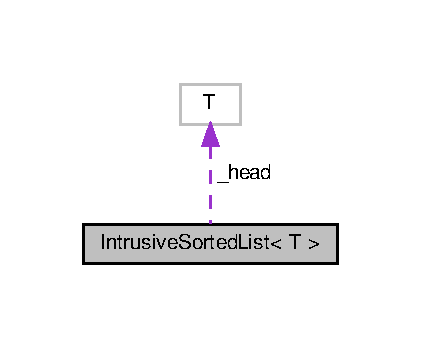
\includegraphics[width=202pt]{d3/da9/classIntrusiveSortedList__coll__graph}
\end{center}
\end{figure}
\subsection*{Classes}
\begin{DoxyCompactItemize}
\item 
struct \hyperlink{structIntrusiveSortedList_1_1Iterator}{Iterator}
\end{DoxyCompactItemize}
\subsection*{Public Member Functions}
\begin{DoxyCompactItemize}
\item 
\mbox{\Hypertarget{classIntrusiveSortedList_a7e0f7c2ef79d4eeee78378bf4c18a8b2}\label{classIntrusiveSortedList_a7e0f7c2ef79d4eeee78378bf4c18a8b2}} 
void {\bfseries add} (T new\+Node)
\item 
\mbox{\Hypertarget{classIntrusiveSortedList_aeed7f2131f31a3a3beb903b2cd435d48}\label{classIntrusiveSortedList_aeed7f2131f31a3a3beb903b2cd435d48}} 
bool {\bfseries remove} (T remove\+Node)
\item 
\mbox{\Hypertarget{classIntrusiveSortedList_a8e3b72bbc6de421d105f0669393fc7a2}\label{classIntrusiveSortedList_a8e3b72bbc6de421d105f0669393fc7a2}} 
\hyperlink{structIntrusiveSortedList_1_1Iterator}{Iterator} {\bfseries begin} ()
\item 
\mbox{\Hypertarget{classIntrusiveSortedList_a5a6ccf96da27b0df5e00ed19bf10fee4}\label{classIntrusiveSortedList_a5a6ccf96da27b0df5e00ed19bf10fee4}} 
\hyperlink{structIntrusiveSortedList_1_1Iterator}{Iterator} {\bfseries end} ()
\item 
\mbox{\Hypertarget{classIntrusiveSortedList_a61b74f65f9ff4288750e57a9d57ef414}\label{classIntrusiveSortedList_a61b74f65f9ff4288750e57a9d57ef414}} 
bool {\bfseries empty} () const
\item 
\mbox{\Hypertarget{classIntrusiveSortedList_a3cd0ec0b219a557286783e0721cee520}\label{classIntrusiveSortedList_a3cd0ec0b219a557286783e0721cee520}} 
size\+\_\+t {\bfseries size} () const
\item 
\mbox{\Hypertarget{classIntrusiveSortedList_a200409fcc5a1b32416052f03ab71f960}\label{classIntrusiveSortedList_a200409fcc5a1b32416052f03ab71f960}} 
void {\bfseries delete\+Node} (T node)
\item 
\mbox{\Hypertarget{classIntrusiveSortedList_a029b06af9123b12532314790f36f53c6}\label{classIntrusiveSortedList_a029b06af9123b12532314790f36f53c6}} 
void {\bfseries clear} ()
\end{DoxyCompactItemize}
\subsection*{Protected Attributes}
\begin{DoxyCompactItemize}
\item 
\mbox{\Hypertarget{classIntrusiveSortedList_a12b97da84a71bb8157907a954ec1490a}\label{classIntrusiveSortedList_a12b97da84a71bb8157907a954ec1490a}} 
T {\bfseries \+\_\+head} \{nullptr\}
\end{DoxyCompactItemize}


\subsection{Detailed Description}
\subsubsection*{template$<$class T$>$\newline
class Intrusive\+Sorted\+List$<$ T $>$}



Definition at line 59 of file Intrusive\+Sorted\+List.\+hpp.



The documentation for this class was generated from the following file\+:\begin{DoxyCompactItemize}
\item 
/home/andressanchez/\+Escritorio/\+G\+I\+T/project\+\_\+template/src/include/containers/\hyperlink{IntrusiveSortedList_8hpp}{Intrusive\+Sorted\+List.\+hpp}\end{DoxyCompactItemize}

\hypertarget{classIntrusiveSortedListNode}{}\section{Intrusive\+Sorted\+List\+Node$<$ T $>$ Class Template Reference}
\label{classIntrusiveSortedListNode}\index{Intrusive\+Sorted\+List\+Node$<$ T $>$@{Intrusive\+Sorted\+List\+Node$<$ T $>$}}


Collaboration diagram for Intrusive\+Sorted\+List\+Node$<$ T $>$\+:\nopagebreak
\begin{figure}[H]
\begin{center}
\leavevmode
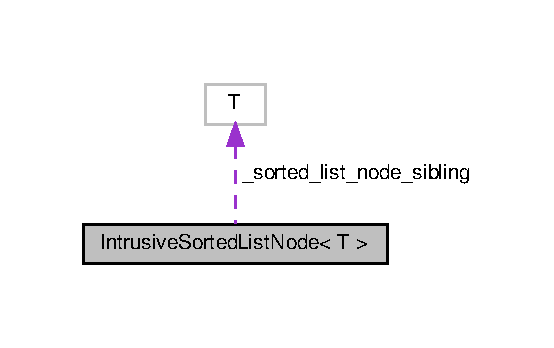
\includegraphics[width=266pt]{d3/d3d/classIntrusiveSortedListNode__coll__graph}
\end{center}
\end{figure}
\subsection*{Public Member Functions}
\begin{DoxyCompactItemize}
\item 
\mbox{\Hypertarget{classIntrusiveSortedListNode_a4f4891e6b0500ad8b81fdb6603b12d4e}\label{classIntrusiveSortedListNode_a4f4891e6b0500ad8b81fdb6603b12d4e}} 
void {\bfseries set\+Sorted\+Sibling} (T sibling)
\item 
\mbox{\Hypertarget{classIntrusiveSortedListNode_ac5fb1a2ec5470b5ca2f2ee13c5f391cb}\label{classIntrusiveSortedListNode_ac5fb1a2ec5470b5ca2f2ee13c5f391cb}} 
const T {\bfseries get\+Sorted\+Sibling} () const
\end{DoxyCompactItemize}
\subsection*{Protected Attributes}
\begin{DoxyCompactItemize}
\item 
\mbox{\Hypertarget{classIntrusiveSortedListNode_a0c80217609ef040929472c44d81e5cd1}\label{classIntrusiveSortedListNode_a0c80217609ef040929472c44d81e5cd1}} 
T {\bfseries \+\_\+sorted\+\_\+list\+\_\+node\+\_\+sibling} \{nullptr\}
\end{DoxyCompactItemize}


\subsection{Detailed Description}
\subsubsection*{template$<$class T$>$\newline
class Intrusive\+Sorted\+List\+Node$<$ T $>$}



Definition at line 49 of file Intrusive\+Sorted\+List.\+hpp.



The documentation for this class was generated from the following file\+:\begin{DoxyCompactItemize}
\item 
/home/andressanchez/\+Escritorio/\+G\+I\+T/project\+\_\+template/src/include/containers/\hyperlink{IntrusiveSortedList_8hpp}{Intrusive\+Sorted\+List.\+hpp}\end{DoxyCompactItemize}

\hypertarget{structIntrusiveSortedList_1_1Iterator}{}\section{Intrusive\+Sorted\+List$<$ T $>$\+:\+:Iterator Struct Reference}
\label{structIntrusiveSortedList_1_1Iterator}\index{Intrusive\+Sorted\+List$<$ T $>$\+::\+Iterator@{Intrusive\+Sorted\+List$<$ T $>$\+::\+Iterator}}


Collaboration diagram for Intrusive\+Sorted\+List$<$ T $>$\+:\+:Iterator\+:\nopagebreak
\begin{figure}[H]
\begin{center}
\leavevmode
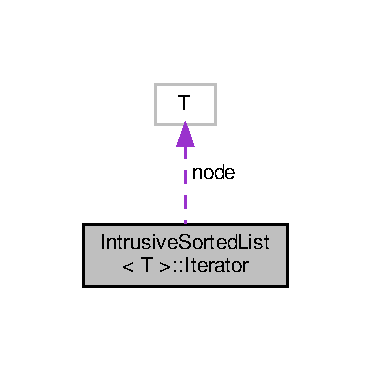
\includegraphics[width=178pt]{db/dab/structIntrusiveSortedList_1_1Iterator__coll__graph}
\end{center}
\end{figure}
\subsection*{Public Member Functions}
\begin{DoxyCompactItemize}
\item 
\mbox{\Hypertarget{structIntrusiveSortedList_1_1Iterator_ab9256df4261a73c93e6408c617176082}\label{structIntrusiveSortedList_1_1Iterator_ab9256df4261a73c93e6408c617176082}} 
{\bfseries Iterator} (T v)
\item 
\mbox{\Hypertarget{structIntrusiveSortedList_1_1Iterator_a22f0efa8317f852d8bc4f8ba44dccd7e}\label{structIntrusiveSortedList_1_1Iterator_a22f0efa8317f852d8bc4f8ba44dccd7e}} 
{\bfseries operator T} () const
\item 
\mbox{\Hypertarget{structIntrusiveSortedList_1_1Iterator_a9c9a2607d2d91b56a4b0a6dc43e8773f}\label{structIntrusiveSortedList_1_1Iterator_a9c9a2607d2d91b56a4b0a6dc43e8773f}} 
{\bfseries operator T\&} ()
\item 
\mbox{\Hypertarget{structIntrusiveSortedList_1_1Iterator_ad5f48f07778b9d2079fac77dcfc1cc86}\label{structIntrusiveSortedList_1_1Iterator_ad5f48f07778b9d2079fac77dcfc1cc86}} 
T {\bfseries operator$\ast$} () const
\item 
\mbox{\Hypertarget{structIntrusiveSortedList_1_1Iterator_a4daeb2b5c9df2555bc99ba6cfe91ad4e}\label{structIntrusiveSortedList_1_1Iterator_a4daeb2b5c9df2555bc99ba6cfe91ad4e}} 
\hyperlink{structIntrusiveSortedList_1_1Iterator}{Iterator} \& {\bfseries operator++} ()
\end{DoxyCompactItemize}
\subsection*{Public Attributes}
\begin{DoxyCompactItemize}
\item 
\mbox{\Hypertarget{structIntrusiveSortedList_1_1Iterator_ac93d1a76a9d6cee80dc0fe7a9e66684b}\label{structIntrusiveSortedList_1_1Iterator_ac93d1a76a9d6cee80dc0fe7a9e66684b}} 
T {\bfseries node}
\end{DoxyCompactItemize}


\subsection{Detailed Description}
\subsubsection*{template$<$class T$>$\newline
struct Intrusive\+Sorted\+List$<$ T $>$\+::\+Iterator}



Definition at line 134 of file Intrusive\+Sorted\+List.\+hpp.



The documentation for this struct was generated from the following file\+:\begin{DoxyCompactItemize}
\item 
/home/andressanchez/\+Escritorio/\+G\+I\+T/project\+\_\+template/src/modules/u\+O\+R\+B/include/containers/\hyperlink{IntrusiveSortedList_8hpp}{Intrusive\+Sorted\+List.\+hpp}\end{DoxyCompactItemize}

\hypertarget{structList_1_1Iterator}{}\section{List$<$ T $>$\+:\+:Iterator Struct Reference}
\label{structList_1_1Iterator}\index{List$<$ T $>$\+::\+Iterator@{List$<$ T $>$\+::\+Iterator}}


Collaboration diagram for List$<$ T $>$\+:\+:Iterator\+:\nopagebreak
\begin{figure}[H]
\begin{center}
\leavevmode
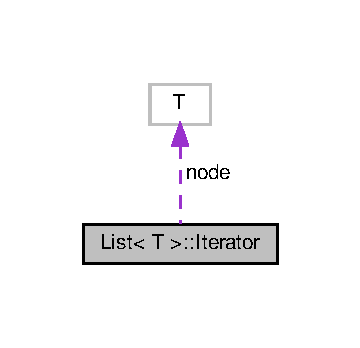
\includegraphics[width=173pt]{da/dcb/structList_1_1Iterator__coll__graph}
\end{center}
\end{figure}
\subsection*{Public Member Functions}
\begin{DoxyCompactItemize}
\item 
\mbox{\Hypertarget{structList_1_1Iterator_a94bfb6df7d896c67b445d87b123aefd3}\label{structList_1_1Iterator_a94bfb6df7d896c67b445d87b123aefd3}} 
{\bfseries Iterator} (T v)
\item 
\mbox{\Hypertarget{structList_1_1Iterator_a25714263a7e0bae6586bbc9edbf47248}\label{structList_1_1Iterator_a25714263a7e0bae6586bbc9edbf47248}} 
{\bfseries operator T} () const
\item 
\mbox{\Hypertarget{structList_1_1Iterator_a64fb726068223f4636be78b3e7296e1b}\label{structList_1_1Iterator_a64fb726068223f4636be78b3e7296e1b}} 
{\bfseries operator T\&} ()
\item 
\mbox{\Hypertarget{structList_1_1Iterator_a212b4cd6a7c78ec53000526da0270fcd}\label{structList_1_1Iterator_a212b4cd6a7c78ec53000526da0270fcd}} 
T {\bfseries operator$\ast$} () const
\item 
\mbox{\Hypertarget{structList_1_1Iterator_a6c0a5a93fe84d4e045ad0256179fc039}\label{structList_1_1Iterator_a6c0a5a93fe84d4e045ad0256179fc039}} 
\hyperlink{structList_1_1Iterator}{Iterator} \& {\bfseries operator++} ()
\end{DoxyCompactItemize}
\subsection*{Public Attributes}
\begin{DoxyCompactItemize}
\item 
\mbox{\Hypertarget{structList_1_1Iterator_acc7d2bcd20a47511a10b7c0cca3bc844}\label{structList_1_1Iterator_acc7d2bcd20a47511a10b7c0cca3bc844}} 
T {\bfseries node}
\end{DoxyCompactItemize}


\subsection{Detailed Description}
\subsubsection*{template$<$class T$>$\newline
struct List$<$ T $>$\+::\+Iterator}



Definition at line 127 of file List.\+hpp.



The documentation for this struct was generated from the following file\+:\begin{DoxyCompactItemize}
\item 
/home/andressanchez/\+Escritorio/\+G\+I\+T/project\+\_\+template/src/include/containers/\hyperlink{List_8hpp}{List.\+hpp}\end{DoxyCompactItemize}

\hypertarget{classList}{}\section{List$<$ T $>$ Class Template Reference}
\label{classList}\index{List$<$ T $>$@{List$<$ T $>$}}
\subsection*{Classes}
\begin{DoxyCompactItemize}
\item 
struct \hyperlink{structList_1_1Iterator}{Iterator}
\end{DoxyCompactItemize}
\subsection*{Public Member Functions}
\begin{DoxyCompactItemize}
\item 
\mbox{\Hypertarget{classList_a3dc06da23dfd238ae00b624e96ba6ada}\label{classList_a3dc06da23dfd238ae00b624e96ba6ada}} 
void {\bfseries add} (T new\+Node)
\item 
\mbox{\Hypertarget{classList_a2202c40ee77a36119bf9db394f06d26d}\label{classList_a2202c40ee77a36119bf9db394f06d26d}} 
bool {\bfseries remove} (T remove\+Node)
\item 
\mbox{\Hypertarget{classList_a3cd86b8318ab6be017fd69a71f1e4874}\label{classList_a3cd86b8318ab6be017fd69a71f1e4874}} 
\hyperlink{structList_1_1Iterator}{Iterator} {\bfseries begin} ()
\item 
\mbox{\Hypertarget{classList_ad860fbbcfb2d693ab4f27fd0aa6125ad}\label{classList_ad860fbbcfb2d693ab4f27fd0aa6125ad}} 
\hyperlink{structList_1_1Iterator}{Iterator} {\bfseries end} ()
\item 
\mbox{\Hypertarget{classList_acfbd04f036ed938f8281c94d1196f0f0}\label{classList_acfbd04f036ed938f8281c94d1196f0f0}} 
const T {\bfseries get\+Head} () const
\item 
\mbox{\Hypertarget{classList_a48efb87cad20cc377b6894f28fa1f3d6}\label{classList_a48efb87cad20cc377b6894f28fa1f3d6}} 
bool {\bfseries empty} () const
\item 
\mbox{\Hypertarget{classList_ae1a21106dc7f2c47c62763a2f6b04f6b}\label{classList_ae1a21106dc7f2c47c62763a2f6b04f6b}} 
size\+\_\+t {\bfseries size} () const
\item 
\mbox{\Hypertarget{classList_a92c3bea8b00f5f84accac07c81f0867d}\label{classList_a92c3bea8b00f5f84accac07c81f0867d}} 
void {\bfseries delete\+Node} (T node)
\item 
\mbox{\Hypertarget{classList_ae296516a252e11963dbf963727ce429a}\label{classList_ae296516a252e11963dbf963727ce429a}} 
void {\bfseries clear} ()
\end{DoxyCompactItemize}
\subsection*{Protected Attributes}
\begin{DoxyCompactItemize}
\item 
\mbox{\Hypertarget{classList_a049bde788f66e78f5ddc762e541f23df}\label{classList_a049bde788f66e78f5ddc762e541f23df}} 
T {\bfseries \+\_\+head} \{nullptr\}
\end{DoxyCompactItemize}


\subsection{Detailed Description}
\subsubsection*{template$<$class T$>$\newline
class List$<$ T $>$}



Definition at line 63 of file List.\+hpp.



The documentation for this class was generated from the following file\+:\begin{DoxyCompactItemize}
\item 
/home/andressanchez/\+Escritorio/\+G\+I\+T/project\+\_\+template/src/include/containers/\hyperlink{List_8hpp}{List.\+hpp}\end{DoxyCompactItemize}

\hypertarget{classListNode}{}\section{List\+Node$<$ T $>$ Class Template Reference}
\label{classListNode}\index{List\+Node$<$ T $>$@{List\+Node$<$ T $>$}}


Collaboration diagram for List\+Node$<$ T $>$\+:\nopagebreak
\begin{figure}[H]
\begin{center}
\leavevmode
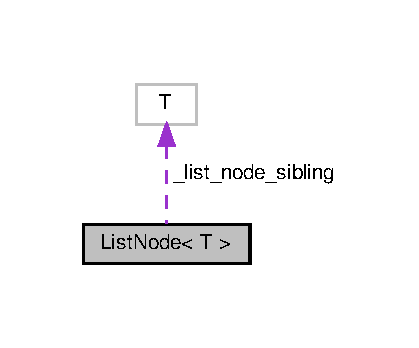
\includegraphics[width=201pt]{d1/da3/classListNode__coll__graph}
\end{center}
\end{figure}
\subsection*{Public Member Functions}
\begin{DoxyCompactItemize}
\item 
\mbox{\Hypertarget{classListNode_a1d1198777d13c405d0a1b696dd735db4}\label{classListNode_a1d1198777d13c405d0a1b696dd735db4}} 
void {\bfseries set\+Sibling} (T sibling)
\item 
\mbox{\Hypertarget{classListNode_a55a754dc43f33886f9c27c9bc20138be}\label{classListNode_a55a754dc43f33886f9c27c9bc20138be}} 
const T {\bfseries get\+Sibling} () const
\end{DoxyCompactItemize}
\subsection*{Protected Attributes}
\begin{DoxyCompactItemize}
\item 
\mbox{\Hypertarget{classListNode_aef40d1d685d22dd9c075bfe77c4e27cf}\label{classListNode_aef40d1d685d22dd9c075bfe77c4e27cf}} 
T {\bfseries \+\_\+list\+\_\+node\+\_\+sibling} \{nullptr\}
\end{DoxyCompactItemize}


\subsection{Detailed Description}
\subsubsection*{template$<$class T$>$\newline
class List\+Node$<$ T $>$}



Definition at line 49 of file List.\+hpp.



The documentation for this class was generated from the following file\+:\begin{DoxyCompactItemize}
\item 
/home/andressanchez/\+Escritorio/\+G\+I\+T/project\+\_\+template/src/include/containers/\hyperlink{List_8hpp}{List.\+hpp}\end{DoxyCompactItemize}

\hypertarget{classLockGuard}{}\section{Lock\+Guard Class Reference}
\label{classLockGuard}\index{Lock\+Guard@{Lock\+Guard}}
\subsection*{Public Member Functions}
\begin{DoxyCompactItemize}
\item 
\mbox{\Hypertarget{classLockGuard_ab02101e6ab27b1a2b078c8cf3b3fca72}\label{classLockGuard_ab02101e6ab27b1a2b078c8cf3b3fca72}} 
{\bfseries Lock\+Guard} (pthread\+\_\+mutex\+\_\+t \&mutex)
\item 
\mbox{\Hypertarget{classLockGuard_aa3b71de031859e32366fac2cde3ebcaf}\label{classLockGuard_aa3b71de031859e32366fac2cde3ebcaf}} 
{\bfseries Lock\+Guard} (const \hyperlink{classLockGuard}{Lock\+Guard} \&other)=delete
\item 
\mbox{\Hypertarget{classLockGuard_ad5cbce17e5d6200c16d2ef0d74e772df}\label{classLockGuard_ad5cbce17e5d6200c16d2ef0d74e772df}} 
\hyperlink{classLockGuard}{Lock\+Guard} \& {\bfseries operator=} (const \hyperlink{classLockGuard}{Lock\+Guard} \&other)=delete
\end{DoxyCompactItemize}


\subsection{Detailed Description}


Definition at line 38 of file Lock\+Guard.\+hpp.



The documentation for this class was generated from the following file\+:\begin{DoxyCompactItemize}
\item 
/home/andressanchez/\+Escritorio/\+G\+I\+T/project\+\_\+template/src/include/containers/Lock\+Guard.\+hpp\end{DoxyCompactItemize}

\hypertarget{classuORB_1_1Manager}{}\section{u\+O\+RB\+:\+:Manager Class Reference}
\label{classuORB_1_1Manager}\index{u\+O\+R\+B\+::\+Manager@{u\+O\+R\+B\+::\+Manager}}


{\ttfamily \#include $<$u\+O\+R\+B\+Manager.\+hpp$>$}

\subsection*{Public Member Functions}
\begin{DoxyCompactItemize}
\item 
\hyperlink{classuORB_1_1DeviceMaster}{u\+O\+R\+B\+::\+Device\+Master} $\ast$ \hyperlink{classuORB_1_1Manager_a083331e24ac4f99ac11a0aab1b1681b4}{get\+\_\+device\+\_\+master} ()
\item 
\hyperlink{uORB_8h_a8d0cfa5f9ea6427a37057d6cea6dd990}{orb\+\_\+advert\+\_\+t} \hyperlink{classuORB_1_1Manager_a42e075fba5970aa0730faab182e2083f}{orb\+\_\+advertise} (const struct \hyperlink{structorb__metadata}{orb\+\_\+metadata} $\ast$meta, const void $\ast$data, unsigned int queue\+\_\+size=1)
\item 
\hyperlink{uORB_8h_a8d0cfa5f9ea6427a37057d6cea6dd990}{orb\+\_\+advert\+\_\+t} \hyperlink{classuORB_1_1Manager_a808104f7ebeab8f0d548dd9127344b24}{orb\+\_\+advertise\+\_\+multi} (const struct \hyperlink{structorb__metadata}{orb\+\_\+metadata} $\ast$meta, const void $\ast$data, int $\ast$instance, unsigned int queue\+\_\+size=1)
\item 
int \hyperlink{classuORB_1_1Manager_a45601ddc722320b9cd660d9548263824}{orb\+\_\+unadvertise} (\hyperlink{uORB_8h_a8d0cfa5f9ea6427a37057d6cea6dd990}{orb\+\_\+advert\+\_\+t} handle)
\item 
int \hyperlink{classuORB_1_1Manager_abbe6966f841886ce3003ebc6d2198447}{orb\+\_\+publish} (const struct \hyperlink{structorb__metadata}{orb\+\_\+metadata} $\ast$meta, \hyperlink{uORB_8h_a8d0cfa5f9ea6427a37057d6cea6dd990}{orb\+\_\+advert\+\_\+t} handle, const void $\ast$data)
\item 
int \hyperlink{classuORB_1_1Manager_ae54072a80ad4de6d127e2dad8182b8fb}{orb\+\_\+subscribe} (const struct \hyperlink{structorb__metadata}{orb\+\_\+metadata} $\ast$meta)
\item 
int \hyperlink{classuORB_1_1Manager_a9a31fb71a0962db44450963559296cfe}{orb\+\_\+subscribe\+\_\+multi} (const struct \hyperlink{structorb__metadata}{orb\+\_\+metadata} $\ast$meta, unsigned instance)
\item 
int \hyperlink{classuORB_1_1Manager_a77539878280b749d79d2c16dc5628c81}{orb\+\_\+unsubscribe} (int handle)
\item 
int \hyperlink{classuORB_1_1Manager_af1048c82b439300c706fe0a083b61f90}{orb\+\_\+copy} (const struct \hyperlink{structorb__metadata}{orb\+\_\+metadata} $\ast$meta, int handle, void $\ast$buffer)
\item 
int \hyperlink{classuORB_1_1Manager_a5503920d25d544ce3be1cf79cda869f7}{orb\+\_\+check} (int handle, bool $\ast$updated)
\item 
int \hyperlink{classuORB_1_1Manager_a446823738a75847a6732008784445c9f}{orb\+\_\+exists} (const struct \hyperlink{structorb__metadata}{orb\+\_\+metadata} $\ast$meta, int instance)
\item 
int \hyperlink{classuORB_1_1Manager_aade04ff2a8a3aaf275b39fc32934fc56}{orb\+\_\+set\+\_\+interval} (int handle, unsigned interval)
\item 
int \hyperlink{classuORB_1_1Manager_a627a7e6ef16970d2b6d8f02471795963}{orb\+\_\+get\+\_\+interval} (int handle, unsigned $\ast$interval)
\end{DoxyCompactItemize}
\subsection*{Static Public Member Functions}
\begin{DoxyCompactItemize}
\item 
static bool \hyperlink{classuORB_1_1Manager_abb160fdd7ba0fe448ffa7f654a796267}{initialize} ()
\item 
static bool \hyperlink{classuORB_1_1Manager_a306a9970d2f7cf304fba4a918e238558}{terminate} ()
\item 
static \hyperlink{classuORB_1_1Manager}{u\+O\+R\+B\+::\+Manager} $\ast$ \hyperlink{classuORB_1_1Manager_a9d829b3ea49d16d03c2fa37ef2bb24a5}{get\+\_\+instance} ()
\end{DoxyCompactItemize}


\subsection{Detailed Description}
This is implemented as a singleton. This class manages creating the u\+O\+RB nodes for each u\+O\+RB topics and also implements the behavor of the u\+O\+RB Api\textquotesingle{}s. 

Definition at line 63 of file u\+O\+R\+B\+Manager.\+hpp.



\subsection{Member Function Documentation}
\mbox{\Hypertarget{classuORB_1_1Manager_a083331e24ac4f99ac11a0aab1b1681b4}\label{classuORB_1_1Manager_a083331e24ac4f99ac11a0aab1b1681b4}} 
\index{u\+O\+R\+B\+::\+Manager@{u\+O\+R\+B\+::\+Manager}!get\+\_\+device\+\_\+master@{get\+\_\+device\+\_\+master}}
\index{get\+\_\+device\+\_\+master@{get\+\_\+device\+\_\+master}!u\+O\+R\+B\+::\+Manager@{u\+O\+R\+B\+::\+Manager}}
\subsubsection{\texorpdfstring{get\+\_\+device\+\_\+master()}{get\_device\_master()}}
{\footnotesize\ttfamily \hyperlink{classuORB_1_1DeviceMaster}{u\+O\+R\+B\+::\+Device\+Master} $\ast$ u\+O\+R\+B\+::\+Manager\+::get\+\_\+device\+\_\+master (\begin{DoxyParamCaption}{ }\end{DoxyParamCaption})}

Get the \hyperlink{classuORB_1_1DeviceMaster}{Device\+Master}. If it does not exist, it will be created and initialized. Note\+: the first call to this is not thread-\/safe. \begin{DoxyReturn}{Returns}
nullptr if initialization failed (and errno will be set) 
\end{DoxyReturn}


Definition at line 90 of file u\+O\+R\+B\+Manager.\+cpp.


\begin{DoxyCode}
91 \{
92     \textcolor{keywordflow}{if} (!\_device\_master) \{
93         \_device\_master = \textcolor{keyword}{new} DeviceMaster();
94 
95         \textcolor{keywordflow}{if} (\_device\_master == \textcolor{keyword}{nullptr}) \{
96             printf(\textcolor{stringliteral}{"Failed to allocate DeviceMaster"});
97             errno = ENOMEM;
98         \}
99     \}
100 
101     \textcolor{keywordflow}{return} \_device\_master;
102 \}
\end{DoxyCode}
\mbox{\Hypertarget{classuORB_1_1Manager_a9d829b3ea49d16d03c2fa37ef2bb24a5}\label{classuORB_1_1Manager_a9d829b3ea49d16d03c2fa37ef2bb24a5}} 
\index{u\+O\+R\+B\+::\+Manager@{u\+O\+R\+B\+::\+Manager}!get\+\_\+instance@{get\+\_\+instance}}
\index{get\+\_\+instance@{get\+\_\+instance}!u\+O\+R\+B\+::\+Manager@{u\+O\+R\+B\+::\+Manager}}
\subsubsection{\texorpdfstring{get\+\_\+instance()}{get\_instance()}}
{\footnotesize\ttfamily static \hyperlink{classuORB_1_1Manager}{u\+O\+R\+B\+::\+Manager}$\ast$ u\+O\+R\+B\+::\+Manager\+::get\+\_\+instance (\begin{DoxyParamCaption}{ }\end{DoxyParamCaption})\hspace{0.3cm}{\ttfamily [inline]}, {\ttfamily [static]}}

Method to get the singleton instance for the \hyperlink{classuORB_1_1Manager}{u\+O\+R\+B\+::\+Manager}. Make sure \hyperlink{classuORB_1_1Manager_abb160fdd7ba0fe448ffa7f654a796267}{initialize()} is called first. \begin{DoxyReturn}{Returns}
\hyperlink{classuORB_1_1Manager}{u\+O\+R\+B\+::\+Manager}$\ast$ 
\end{DoxyReturn}


Definition at line 88 of file u\+O\+R\+B\+Manager.\+hpp.


\begin{DoxyCode}
88 \{ \textcolor{keywordflow}{return} \_Instance; \}
\end{DoxyCode}
\mbox{\Hypertarget{classuORB_1_1Manager_abb160fdd7ba0fe448ffa7f654a796267}\label{classuORB_1_1Manager_abb160fdd7ba0fe448ffa7f654a796267}} 
\index{u\+O\+R\+B\+::\+Manager@{u\+O\+R\+B\+::\+Manager}!initialize@{initialize}}
\index{initialize@{initialize}!u\+O\+R\+B\+::\+Manager@{u\+O\+R\+B\+::\+Manager}}
\subsubsection{\texorpdfstring{initialize()}{initialize()}}
{\footnotesize\ttfamily bool u\+O\+R\+B\+::\+Manager\+::initialize (\begin{DoxyParamCaption}{ }\end{DoxyParamCaption})\hspace{0.3cm}{\ttfamily [static]}}

Initialize the singleton. Call this before everything else. \begin{DoxyReturn}{Returns}
true on success 
\end{DoxyReturn}


Definition at line 47 of file u\+O\+R\+B\+Manager.\+cpp.


\begin{DoxyCode}
48 \{
49     \textcolor{keywordflow}{if} (\_Instance == \textcolor{keyword}{nullptr}) \{
50         \_Instance = \textcolor{keyword}{new} \hyperlink{classuORB_1_1Manager}{uORB::Manager}();
51     \}
52 
53     \textcolor{keywordflow}{return} \_Instance != \textcolor{keyword}{nullptr};
54 \}
\end{DoxyCode}
\mbox{\Hypertarget{classuORB_1_1Manager_a42e075fba5970aa0730faab182e2083f}\label{classuORB_1_1Manager_a42e075fba5970aa0730faab182e2083f}} 
\index{u\+O\+R\+B\+::\+Manager@{u\+O\+R\+B\+::\+Manager}!orb\+\_\+advertise@{orb\+\_\+advertise}}
\index{orb\+\_\+advertise@{orb\+\_\+advertise}!u\+O\+R\+B\+::\+Manager@{u\+O\+R\+B\+::\+Manager}}
\subsubsection{\texorpdfstring{orb\+\_\+advertise()}{orb\_advertise()}}
{\footnotesize\ttfamily \hyperlink{uORB_8h_a8d0cfa5f9ea6427a37057d6cea6dd990}{orb\+\_\+advert\+\_\+t} u\+O\+R\+B\+::\+Manager\+::orb\+\_\+advertise (\begin{DoxyParamCaption}\item[{const struct \hyperlink{structorb__metadata}{orb\+\_\+metadata} $\ast$}]{meta,  }\item[{const void $\ast$}]{data,  }\item[{unsigned int}]{queue\+\_\+size = {\ttfamily 1} }\end{DoxyParamCaption})\hspace{0.3cm}{\ttfamily [inline]}}

Advertise as the publisher of a topic.

This performs the initial advertisement of a topic; it creates the topic node in /obj if required and publishes the initial data.

Any number of advertisers may publish to a topic; publications are atomic but co-\/ordination between publishers is not provided by the O\+RB.

Internally this will call orb\+\_\+advertise\+\_\+multi with an instance of 0.


\begin{DoxyParams}{Parameters}
{\em meta} & The u\+O\+RB metadata (usually from the \hyperlink{uORB_8h_a96af5434ec1acdf24287bd7851b0413f}{O\+R\+B\+\_\+\+I\+D()} macro) for the topic. \\
\hline
{\em data} & A pointer to the initial data to be published. For topics updated by interrupt handlers, the advertisement must be performed from non-\/interrupt context. \\
\hline
{\em queue\+\_\+size} & Maximum number of buffered elements. If this is 1, no queuing is used. \\
\hline
\end{DoxyParams}
\begin{DoxyReturn}{Returns}
nullptr on error, otherwise returns an object pointer that can be used to publish to the topic. If the topic in question is not known (due to an O\+R\+B\+\_\+\+D\+E\+F\+I\+NE with no corresponding O\+R\+B\+\_\+\+D\+E\+C\+L\+A\+RE) this function will return nullptr and set errno to E\+N\+O\+E\+NT. 
\end{DoxyReturn}


Definition at line 123 of file u\+O\+R\+B\+Manager.\+hpp.


\begin{DoxyCode}
124     \{
125         \textcolor{keywordflow}{return} \hyperlink{classuORB_1_1Manager_a808104f7ebeab8f0d548dd9127344b24}{orb\_advertise\_multi}(meta, data, \textcolor{keyword}{nullptr}, queue\_size);
126     \}
\end{DoxyCode}
\mbox{\Hypertarget{classuORB_1_1Manager_a808104f7ebeab8f0d548dd9127344b24}\label{classuORB_1_1Manager_a808104f7ebeab8f0d548dd9127344b24}} 
\index{u\+O\+R\+B\+::\+Manager@{u\+O\+R\+B\+::\+Manager}!orb\+\_\+advertise\+\_\+multi@{orb\+\_\+advertise\+\_\+multi}}
\index{orb\+\_\+advertise\+\_\+multi@{orb\+\_\+advertise\+\_\+multi}!u\+O\+R\+B\+::\+Manager@{u\+O\+R\+B\+::\+Manager}}
\subsubsection{\texorpdfstring{orb\+\_\+advertise\+\_\+multi()}{orb\_advertise\_multi()}}
{\footnotesize\ttfamily \hyperlink{uORB_8h_a8d0cfa5f9ea6427a37057d6cea6dd990}{orb\+\_\+advert\+\_\+t} u\+O\+R\+B\+::\+Manager\+::orb\+\_\+advertise\+\_\+multi (\begin{DoxyParamCaption}\item[{const struct \hyperlink{structorb__metadata}{orb\+\_\+metadata} $\ast$}]{meta,  }\item[{const void $\ast$}]{data,  }\item[{int $\ast$}]{instance,  }\item[{unsigned int}]{queue\+\_\+size = {\ttfamily 1} }\end{DoxyParamCaption})}

Advertise as the publisher of a topic.

This performs the initial advertisement of a topic; it creates the topic node in /obj if required and publishes the initial data.

Any number of advertisers may publish to a topic; publications are atomic but co-\/ordination between publishers is not provided by the O\+RB.

The multi can be used to create multiple independent instances of the same topic (each instance has its own buffer). This is useful for multiple publishers who publish the same topic. The subscriber then subscribes to all instances and chooses which source he wants to use.


\begin{DoxyParams}{Parameters}
{\em meta} & The u\+O\+RB metadata (usually from the \hyperlink{uORB_8h_a96af5434ec1acdf24287bd7851b0413f}{O\+R\+B\+\_\+\+I\+D()} macro) for the topic. \\
\hline
{\em data} & A pointer to the initial data to be published. For topics updated by interrupt handlers, the advertisement must be performed from non-\/interrupt context. \\
\hline
{\em instance} & Pointer to an integer which will yield the instance ID (0-\/based) of the publication. This is an output parameter and will be set to the newly created instance, ie. 0 for the first advertiser, 1 for the next and so on. \\
\hline
{\em queue\+\_\+size} & Maximum number of buffered elements. If this is 1, no queuing is used. \\
\hline
\end{DoxyParams}
\begin{DoxyReturn}{Returns}
P\+X4\+\_\+\+E\+R\+R\+OR on error, otherwise returns a handle that can be used to publish to the topic. If the topic in question is not known (due to an O\+R\+B\+\_\+\+D\+E\+F\+I\+NE with no corresponding O\+R\+B\+\_\+\+D\+E\+C\+L\+A\+RE) this function will return -\/1 and set errno to E\+N\+O\+E\+NT. 
\end{DoxyReturn}


Definition at line 168 of file u\+O\+R\+B\+Manager.\+cpp.


\begin{DoxyCode}
170 \{
171 \textcolor{preprocessor}{#ifdef ORB\_USE\_PUBLISHER\_RULES}
172 
173     \textcolor{comment}{// check publisher rule}
174     \textcolor{keywordflow}{if} (\_has\_publisher\_rules) \{
175         \textcolor{keyword}{const} \textcolor{keywordtype}{char} *prog\_name = px4\_get\_taskname();
176 
177         \textcolor{keywordflow}{if} (strcmp(\_publisher\_rule.module\_name, prog\_name) == 0) \{
178             \textcolor{keywordflow}{if} (\_publisher\_rule.ignore\_other\_topics) \{
179                 \textcolor{keywordflow}{if} (!findTopic(\_publisher\_rule, meta->\hyperlink{structorb__metadata_a54d1751f24aa0c1f24934c6712811e58}{o\_name})) \{
180                     PX4\_DEBUG(\textcolor{stringliteral}{"not allowing %s to publish topic %s"}, prog\_name, meta->
      \hyperlink{structorb__metadata_a54d1751f24aa0c1f24934c6712811e58}{o\_name});
181                     \textcolor{keywordflow}{return} (\hyperlink{uORB_8h_a8d0cfa5f9ea6427a37057d6cea6dd990}{orb\_advert\_t})\_Instance;
182                 \}
183             \}
184 
185         \} \textcolor{keywordflow}{else} \{
186             \textcolor{keywordflow}{if} (findTopic(\_publisher\_rule, meta->\hyperlink{structorb__metadata_a54d1751f24aa0c1f24934c6712811e58}{o\_name})) \{
187                 PX4\_DEBUG(\textcolor{stringliteral}{"not allowing %s to publish topic %s"}, prog\_name, meta->
      \hyperlink{structorb__metadata_a54d1751f24aa0c1f24934c6712811e58}{o\_name});
188                 \textcolor{keywordflow}{return} (\hyperlink{uORB_8h_a8d0cfa5f9ea6427a37057d6cea6dd990}{orb\_advert\_t})\_Instance;
189             \}
190         \}
191     \}
192 
193 \textcolor{preprocessor}{#endif }\textcolor{comment}{/* ORB\_USE\_PUBLISHER\_RULES */}\textcolor{preprocessor}{}
194 
195     \textcolor{comment}{/* open the node as an advertiser */}
196     \textcolor{keywordtype}{int} fd = node\_open(meta, \textcolor{keyword}{true}, instance);
197 
198     \textcolor{keywordflow}{if} (fd == -1) \{
199         printf(\textcolor{stringliteral}{"%s advertise failed (%i)"}, meta->\hyperlink{structorb__metadata_a54d1751f24aa0c1f24934c6712811e58}{o\_name}, errno);
200         \textcolor{keywordflow}{return} \textcolor{keyword}{nullptr};
201     \}
202 
203     \textcolor{comment}{/* Set the queue size. This must be done before the first publication; thus it fails if}
204 \textcolor{comment}{     * this is not the first advertiser.}
205 \textcolor{comment}{     */}
206     \textcolor{keywordtype}{int} result = ioctl(fd, \hyperlink{drv__orb__dev_8h_a4835f9286d5aac7a6b5e0a01661cbee7}{ORBIOCSETQUEUESIZE}, (\textcolor{keywordtype}{unsigned} \textcolor{keywordtype}{long})queue\_size);
207 
208     \textcolor{keywordflow}{if} (result < 0 && queue\_size > 1) \{
209         printf(\textcolor{stringliteral}{"orb\_advertise\_multi: failed to set queue size"});
210     \}
211 
212     \textcolor{comment}{/* get the advertiser handle and close the node */}
213     \hyperlink{uORB_8h_a8d0cfa5f9ea6427a37057d6cea6dd990}{orb\_advert\_t} advertiser;
214 
215     result = ioctl(fd, \hyperlink{drv__orb__dev_8h_a0ba7c1d8b06e6930ed9589dbebbc775a}{ORBIOCGADVERTISER}, (\textcolor{keywordtype}{unsigned} \textcolor{keywordtype}{long})&advertiser);
216     close(fd);
217 
218     \textcolor{keywordflow}{if} (result == -1) \{
219         printf(\textcolor{stringliteral}{"px4\_ioctl ORBIOCGADVERTISER failed. fd = %d"}, fd);
220         \textcolor{keywordflow}{return} \textcolor{keyword}{nullptr};
221     \}
222 
223 \textcolor{preprocessor}{#ifdef ORB\_COMMUNICATOR}
224     \textcolor{comment}{// For remote systems call over and inform them}
225     uORB::DeviceNode::topic\_advertised(meta);
226 \textcolor{preprocessor}{#endif }\textcolor{comment}{/* ORB\_COMMUNICATOR */}\textcolor{preprocessor}{}
227 
228     \textcolor{comment}{/* the advertiser may perform an initial publish to initialise the object */}
229     \textcolor{keywordflow}{if} (data != \textcolor{keyword}{nullptr}) \{
230         result = \hyperlink{classuORB_1_1Manager_abbe6966f841886ce3003ebc6d2198447}{orb\_publish}(meta, advertiser, data);
231 
232         \textcolor{keywordflow}{if} (result == -1) \{
233             printf(\textcolor{stringliteral}{"orb\_publish failed %s"}, meta->\hyperlink{structorb__metadata_a54d1751f24aa0c1f24934c6712811e58}{o\_name});
234             \textcolor{keywordflow}{return} \textcolor{keyword}{nullptr};
235         \}
236     \}
237 
238     \textcolor{keywordflow}{return} advertiser;
239 \}
\end{DoxyCode}
\mbox{\Hypertarget{classuORB_1_1Manager_a5503920d25d544ce3be1cf79cda869f7}\label{classuORB_1_1Manager_a5503920d25d544ce3be1cf79cda869f7}} 
\index{u\+O\+R\+B\+::\+Manager@{u\+O\+R\+B\+::\+Manager}!orb\+\_\+check@{orb\+\_\+check}}
\index{orb\+\_\+check@{orb\+\_\+check}!u\+O\+R\+B\+::\+Manager@{u\+O\+R\+B\+::\+Manager}}
\subsubsection{\texorpdfstring{orb\+\_\+check()}{orb\_check()}}
{\footnotesize\ttfamily int u\+O\+R\+B\+::\+Manager\+::orb\+\_\+check (\begin{DoxyParamCaption}\item[{int}]{handle,  }\item[{bool $\ast$}]{updated }\end{DoxyParamCaption})}

Check whether a topic has been published to since the last orb\+\_\+copy.

This check can be used to determine whether to copy the topic when not using poll(), or to avoid the overhead of calling poll() when the topic is likely to have updated.

Updates are tracked on a per-\/handle basis; this call will continue to return true until orb\+\_\+copy is called using the same handle.


\begin{DoxyParams}{Parameters}
{\em handle} & A handle returned from orb\+\_\+subscribe. \\
\hline
{\em updated} & Set to true if the topic has been updated since the last time it was copied using this handle. \\
\hline
\end{DoxyParams}
\begin{DoxyReturn}{Returns}
OK if the check was successful, P\+X4\+\_\+\+E\+R\+R\+OR otherwise with errno set accordingly. 
\end{DoxyReturn}


Definition at line 301 of file u\+O\+R\+B\+Manager.\+cpp.


\begin{DoxyCode}
302 \{
303     \textcolor{comment}{/* Set to false here so that if `px4\_ioctl` fails to false. */}
304     *updated = \textcolor{keyword}{false};
305     \textcolor{keywordflow}{return} ioctl(handle, \hyperlink{drv__orb__dev_8h_a60e19540d21f9a44e9157804121957f8}{ORBIOCUPDATED}, (\textcolor{keywordtype}{unsigned} \textcolor{keywordtype}{long})(uintptr\_t)updated);
306 \}
\end{DoxyCode}
\mbox{\Hypertarget{classuORB_1_1Manager_af1048c82b439300c706fe0a083b61f90}\label{classuORB_1_1Manager_af1048c82b439300c706fe0a083b61f90}} 
\index{u\+O\+R\+B\+::\+Manager@{u\+O\+R\+B\+::\+Manager}!orb\+\_\+copy@{orb\+\_\+copy}}
\index{orb\+\_\+copy@{orb\+\_\+copy}!u\+O\+R\+B\+::\+Manager@{u\+O\+R\+B\+::\+Manager}}
\subsubsection{\texorpdfstring{orb\+\_\+copy()}{orb\_copy()}}
{\footnotesize\ttfamily int u\+O\+R\+B\+::\+Manager\+::orb\+\_\+copy (\begin{DoxyParamCaption}\item[{const struct \hyperlink{structorb__metadata}{orb\+\_\+metadata} $\ast$}]{meta,  }\item[{int}]{handle,  }\item[{void $\ast$}]{buffer }\end{DoxyParamCaption})}

Fetch data from a topic.

This is the only operation that will reset the internal marker that indicates that a topic has been updated for a subscriber. Once poll or check return indicating that an updaet is available, this call must be used to update the subscription.


\begin{DoxyParams}{Parameters}
{\em meta} & The u\+O\+RB metadata (usually from the \hyperlink{uORB_8h_a96af5434ec1acdf24287bd7851b0413f}{O\+R\+B\+\_\+\+I\+D()} macro) for the topic. \\
\hline
{\em handle} & A handle returned from orb\+\_\+subscribe. \\
\hline
{\em buffer} & Pointer to the buffer receiving the data, or N\+U\+LL if the caller wants to clear the updated flag without using the data. \\
\hline
\end{DoxyParams}
\begin{DoxyReturn}{Returns}
OK on success, P\+X4\+\_\+\+E\+R\+R\+OR otherwise with errno set accordingly. 
\end{DoxyReturn}


Definition at line 283 of file u\+O\+R\+B\+Manager.\+cpp.


\begin{DoxyCode}
284 \{
285     \textcolor{keywordtype}{int} ret;
286 
287     ret = read(handle, buffer, meta->\hyperlink{structorb__metadata_a400a86fe707613e881b620cde7888b74}{o\_size});
288 
289     \textcolor{keywordflow}{if} (ret < 0) \{
290         \textcolor{keywordflow}{return} -1;
291     \}
292 
293     \textcolor{keywordflow}{if} (ret != (\textcolor{keywordtype}{int})meta->\hyperlink{structorb__metadata_a400a86fe707613e881b620cde7888b74}{o\_size}) \{
294         errno = EIO;
295         \textcolor{keywordflow}{return} -1;
296     \}
297 
298     \textcolor{keywordflow}{return} 0;
299 \}
\end{DoxyCode}
\mbox{\Hypertarget{classuORB_1_1Manager_a446823738a75847a6732008784445c9f}\label{classuORB_1_1Manager_a446823738a75847a6732008784445c9f}} 
\index{u\+O\+R\+B\+::\+Manager@{u\+O\+R\+B\+::\+Manager}!orb\+\_\+exists@{orb\+\_\+exists}}
\index{orb\+\_\+exists@{orb\+\_\+exists}!u\+O\+R\+B\+::\+Manager@{u\+O\+R\+B\+::\+Manager}}
\subsubsection{\texorpdfstring{orb\+\_\+exists()}{orb\_exists()}}
{\footnotesize\ttfamily int u\+O\+R\+B\+::\+Manager\+::orb\+\_\+exists (\begin{DoxyParamCaption}\item[{const struct \hyperlink{structorb__metadata}{orb\+\_\+metadata} $\ast$}]{meta,  }\item[{int}]{instance }\end{DoxyParamCaption})}

Check if a topic has already been created and published (advertised)


\begin{DoxyParams}{Parameters}
{\em meta} & O\+RB topic metadata. \\
\hline
{\em instance} & O\+RB instance \\
\hline
\end{DoxyParams}
\begin{DoxyReturn}{Returns}
OK if the topic exists, P\+X4\+\_\+\+E\+R\+R\+OR otherwise. 
\end{DoxyReturn}


Definition at line 104 of file u\+O\+R\+B\+Manager.\+cpp.


\begin{DoxyCode}
105 \{
106     \textcolor{keywordtype}{int} ret = -1;
107 
108     \textcolor{comment}{// instance valid range: [0, ORB\_MULTI\_MAX\_INSTANCES)}
109     \textcolor{keywordflow}{if} ((instance < 0) || (instance > (\hyperlink{uORB_8h_a8c09e8f28a090e8cae61e10d627f102a}{ORB\_MULTI\_MAX\_INSTANCES} - 1))) \{
110         \textcolor{keywordflow}{return} ret;
111     \}
112 
113     \textcolor{keywordflow}{if} (\hyperlink{classuORB_1_1Manager_a083331e24ac4f99ac11a0aab1b1681b4}{get\_device\_master}()) \{
114         \hyperlink{classuORB_1_1DeviceNode}{uORB::DeviceNode} *node = \_device\_master->\hyperlink{classuORB_1_1DeviceMaster_a793df66a48dcabdd0f5bd8c85beee13c}{getDeviceNode}(meta, instance)
      ;
115 
116         \textcolor{keywordflow}{if} (node != \textcolor{keyword}{nullptr}) \{
117             \textcolor{keywordflow}{if} (node->\hyperlink{classuORB_1_1DeviceNode_a16d1880bc99853428a8d8a240f24857b}{is\_advertised}()) \{
118                 \textcolor{keywordflow}{return} 0;
119             \}
120         \}
121     \}
122 
123 \textcolor{preprocessor}{#ifdef ORB\_COMMUNICATOR}
124 
125     \textcolor{comment}{/*}
126 \textcolor{comment}{     * Generate the path to the node and try to open it.}
127 \textcolor{comment}{     */}
128     \textcolor{keywordtype}{char} path[orb\_maxpath];
129     \textcolor{keywordtype}{int} inst = instance;
130 
131     ret = uORB::Utils::node\_mkpath(path, meta, &inst);
132 
133     \textcolor{keywordflow}{if} (ret != OK) \{
134         errno = -ret;
135         \textcolor{keywordflow}{return} PX4\_ERROR;
136     \}
137 
138     ret = px4\_access(path, F\_OK);
139 
140     \textcolor{keywordflow}{if} (ret == -1 && meta != \textcolor{keyword}{nullptr} && !\_remote\_topics.empty()) \{
141         ret = (\_remote\_topics.find(meta->\hyperlink{structorb__metadata_a54d1751f24aa0c1f24934c6712811e58}{o\_name}) != \_remote\_topics.end()) ? OK : PX4\_ERROR;
142     \}
143 
144     \textcolor{keywordflow}{if} (ret == 0) \{
145         \textcolor{comment}{// we know the topic exists, but it's not necessarily advertised/published yet (for example}
146         \textcolor{comment}{// if there is only a subscriber)}
147         \textcolor{comment}{// The open() will not lead to memory allocations.}
148         \textcolor{keywordtype}{int} fd = px4\_open(path, 0);
149 
150         \textcolor{keywordflow}{if} (fd >= 0) \{
151             \textcolor{keywordtype}{unsigned} \textcolor{keywordtype}{long} is\_advertised;
152 
153             \textcolor{keywordflow}{if} (px4\_ioctl(fd, \hyperlink{drv__orb__dev_8h_a00f4a4fca062412c74b581a041c43c7a}{ORBIOCISADVERTISED}, (\textcolor{keywordtype}{unsigned} \textcolor{keywordtype}{long})&is\_advertised) == 0) \{
154                 \textcolor{keywordflow}{if} (!is\_advertised) \{
155                     ret = PX4\_ERROR;
156                 \}
157             \}
158 
159             px4\_close(fd);
160         \}
161     \}
162 
163 \textcolor{preprocessor}{#endif }\textcolor{comment}{/* ORB\_COMMUNICATOR */}\textcolor{preprocessor}{}
164 
165     \textcolor{keywordflow}{return} ret;
166 \}
\end{DoxyCode}
\mbox{\Hypertarget{classuORB_1_1Manager_a627a7e6ef16970d2b6d8f02471795963}\label{classuORB_1_1Manager_a627a7e6ef16970d2b6d8f02471795963}} 
\index{u\+O\+R\+B\+::\+Manager@{u\+O\+R\+B\+::\+Manager}!orb\+\_\+get\+\_\+interval@{orb\+\_\+get\+\_\+interval}}
\index{orb\+\_\+get\+\_\+interval@{orb\+\_\+get\+\_\+interval}!u\+O\+R\+B\+::\+Manager@{u\+O\+R\+B\+::\+Manager}}
\subsubsection{\texorpdfstring{orb\+\_\+get\+\_\+interval()}{orb\_get\_interval()}}
{\footnotesize\ttfamily int u\+O\+R\+B\+::\+Manager\+::orb\+\_\+get\+\_\+interval (\begin{DoxyParamCaption}\item[{int}]{handle,  }\item[{unsigned $\ast$}]{interval }\end{DoxyParamCaption})}

Get the minimum interval between which updates are seen for a subscription.

\begin{DoxySeeAlso}{See also}
\hyperlink{classuORB_1_1Manager_aade04ff2a8a3aaf275b39fc32934fc56}{orb\+\_\+set\+\_\+interval()}
\end{DoxySeeAlso}

\begin{DoxyParams}{Parameters}
{\em handle} & A handle returned from orb\+\_\+subscribe. \\
\hline
{\em interval} & The returned interval period in milliseconds. \\
\hline
\end{DoxyParams}
\begin{DoxyReturn}{Returns}
OK on success, P\+X4\+\_\+\+E\+R\+R\+OR otherwise with E\+R\+R\+NO set accordingly. 
\end{DoxyReturn}


Definition at line 313 of file u\+O\+R\+B\+Manager.\+cpp.


\begin{DoxyCode}
314 \{
315     \textcolor{keywordtype}{int} ret = ioctl(handle, \hyperlink{drv__orb__dev_8h_acdbdb0d6f9b8600498ffa2599dca742d}{ORBIOCGETINTERVAL}, (\textcolor{keywordtype}{unsigned} \textcolor{keywordtype}{long})interval);
316     *interval /= 1000;
317     \textcolor{keywordflow}{return} ret;
318 \}
\end{DoxyCode}
\mbox{\Hypertarget{classuORB_1_1Manager_abbe6966f841886ce3003ebc6d2198447}\label{classuORB_1_1Manager_abbe6966f841886ce3003ebc6d2198447}} 
\index{u\+O\+R\+B\+::\+Manager@{u\+O\+R\+B\+::\+Manager}!orb\+\_\+publish@{orb\+\_\+publish}}
\index{orb\+\_\+publish@{orb\+\_\+publish}!u\+O\+R\+B\+::\+Manager@{u\+O\+R\+B\+::\+Manager}}
\subsubsection{\texorpdfstring{orb\+\_\+publish()}{orb\_publish()}}
{\footnotesize\ttfamily int u\+O\+R\+B\+::\+Manager\+::orb\+\_\+publish (\begin{DoxyParamCaption}\item[{const struct \hyperlink{structorb__metadata}{orb\+\_\+metadata} $\ast$}]{meta,  }\item[{\hyperlink{uORB_8h_a8d0cfa5f9ea6427a37057d6cea6dd990}{orb\+\_\+advert\+\_\+t}}]{handle,  }\item[{const void $\ast$}]{data }\end{DoxyParamCaption})}

Publish new data to a topic.

The data is atomically published to the topic and any waiting subscribers will be notified. Subscribers that are not waiting can check the topic for updates using orb\+\_\+check.


\begin{DoxyParams}{Parameters}
{\em meta} & The u\+O\+RB metadata (usually from the \hyperlink{uORB_8h_a96af5434ec1acdf24287bd7851b0413f}{O\+R\+B\+\_\+\+I\+D()} macro) for the topic.  The handle returned from orb\+\_\+advertise. \\
\hline
{\em data} & A pointer to the data to be published. \\
\hline
\end{DoxyParams}
\begin{DoxyReturn}{Returns}
OK on success, P\+X4\+\_\+\+E\+R\+R\+OR otherwise with errno set accordingly. 
\end{DoxyReturn}


Definition at line 270 of file u\+O\+R\+B\+Manager.\+cpp.


\begin{DoxyCode}
271 \{
272 \textcolor{preprocessor}{#ifdef ORB\_USE\_PUBLISHER\_RULES}
273 
274     \textcolor{keywordflow}{if} (handle == \_Instance) \{
275         \textcolor{keywordflow}{return} PX4\_OK; \textcolor{comment}{//pretend success}
276     \}
277 
278 \textcolor{preprocessor}{#endif }\textcolor{comment}{/* ORB\_USE\_PUBLISHER\_RULES */}\textcolor{preprocessor}{}
279 
280     \textcolor{keywordflow}{return} \hyperlink{classuORB_1_1DeviceNode_ae715517a1f3a2f361e37d061b59a4560}{uORB::DeviceNode::publish}(meta, handle, data);
281 \}
\end{DoxyCode}
\mbox{\Hypertarget{classuORB_1_1Manager_aade04ff2a8a3aaf275b39fc32934fc56}\label{classuORB_1_1Manager_aade04ff2a8a3aaf275b39fc32934fc56}} 
\index{u\+O\+R\+B\+::\+Manager@{u\+O\+R\+B\+::\+Manager}!orb\+\_\+set\+\_\+interval@{orb\+\_\+set\+\_\+interval}}
\index{orb\+\_\+set\+\_\+interval@{orb\+\_\+set\+\_\+interval}!u\+O\+R\+B\+::\+Manager@{u\+O\+R\+B\+::\+Manager}}
\subsubsection{\texorpdfstring{orb\+\_\+set\+\_\+interval()}{orb\_set\_interval()}}
{\footnotesize\ttfamily int u\+O\+R\+B\+::\+Manager\+::orb\+\_\+set\+\_\+interval (\begin{DoxyParamCaption}\item[{int}]{handle,  }\item[{unsigned}]{interval }\end{DoxyParamCaption})}

Set the minimum interval between which updates are seen for a subscription.

If this interval is set, the subscriber will not see more than one update within the period.

Specifically, the first time an update is reported to the subscriber a timer is started. The update will continue to be reported via poll and orb\+\_\+check, but once fetched via orb\+\_\+copy another update will not be reported until the timer expires.

This feature can be used to pace a subscriber that is watching a topic that would otherwise update too quickly.


\begin{DoxyParams}{Parameters}
{\em handle} & A handle returned from orb\+\_\+subscribe. \\
\hline
{\em interval} & An interval period in milliseconds. \\
\hline
\end{DoxyParams}
\begin{DoxyReturn}{Returns}
OK on success, P\+X4\+\_\+\+E\+R\+R\+OR otherwise with E\+R\+R\+NO set accordingly. 
\end{DoxyReturn}


Definition at line 308 of file u\+O\+R\+B\+Manager.\+cpp.


\begin{DoxyCode}
309 \{
310     \textcolor{keywordflow}{return} ioctl(handle, \hyperlink{drv__orb__dev_8h_a815da46533c3937c84c1496218659d0b}{ORBIOCSETINTERVAL}, interval * 1000);
311 \}
\end{DoxyCode}
\mbox{\Hypertarget{classuORB_1_1Manager_ae54072a80ad4de6d127e2dad8182b8fb}\label{classuORB_1_1Manager_ae54072a80ad4de6d127e2dad8182b8fb}} 
\index{u\+O\+R\+B\+::\+Manager@{u\+O\+R\+B\+::\+Manager}!orb\+\_\+subscribe@{orb\+\_\+subscribe}}
\index{orb\+\_\+subscribe@{orb\+\_\+subscribe}!u\+O\+R\+B\+::\+Manager@{u\+O\+R\+B\+::\+Manager}}
\subsubsection{\texorpdfstring{orb\+\_\+subscribe()}{orb\_subscribe()}}
{\footnotesize\ttfamily int u\+O\+R\+B\+::\+Manager\+::orb\+\_\+subscribe (\begin{DoxyParamCaption}\item[{const struct \hyperlink{structorb__metadata}{orb\+\_\+metadata} $\ast$}]{meta }\end{DoxyParamCaption})}

Subscribe to a topic.

The returned value is a file descriptor that can be passed to poll() in order to wait for updates to a topic, as well as topic\+\_\+read, orb\+\_\+check.

If there were any publications of the topic prior to the subscription, an orb\+\_\+check right after orb\+\_\+subscribe will return true.

\hyperlink{classuORB_1_1Subscription}{Subscription} will succeed even if the topic has not been advertised; in this case the topic will have a timestamp of zero, it will never signal a poll() event, checking will always return false and it cannot be copied. When the topic is subsequently advertised, poll, check, stat and copy calls will react to the initial publication that is performed as part of the advertisement.

\hyperlink{classuORB_1_1Subscription}{Subscription} will fail if the topic is not known to the system, i.\+e. there is nothing in the system that has declared the topic and thus it can never be published.

Internally this will call orb\+\_\+subscribe\+\_\+multi with instance 0.


\begin{DoxyParams}{Parameters}
{\em meta} & The u\+O\+RB metadata (usually from the \hyperlink{uORB_8h_a96af5434ec1acdf24287bd7851b0413f}{O\+R\+B\+\_\+\+I\+D()} macro) for the topic. \\
\hline
\end{DoxyParams}
\begin{DoxyReturn}{Returns}
P\+X4\+\_\+\+E\+R\+R\+OR on error, otherwise returns a handle that can be used to read and update the topic. 
\end{DoxyReturn}


Definition at line 254 of file u\+O\+R\+B\+Manager.\+cpp.


\begin{DoxyCode}
255 \{
256     \textcolor{keywordflow}{return} node\_open(meta, \textcolor{keyword}{false});
257 \}
\end{DoxyCode}
\mbox{\Hypertarget{classuORB_1_1Manager_a9a31fb71a0962db44450963559296cfe}\label{classuORB_1_1Manager_a9a31fb71a0962db44450963559296cfe}} 
\index{u\+O\+R\+B\+::\+Manager@{u\+O\+R\+B\+::\+Manager}!orb\+\_\+subscribe\+\_\+multi@{orb\+\_\+subscribe\+\_\+multi}}
\index{orb\+\_\+subscribe\+\_\+multi@{orb\+\_\+subscribe\+\_\+multi}!u\+O\+R\+B\+::\+Manager@{u\+O\+R\+B\+::\+Manager}}
\subsubsection{\texorpdfstring{orb\+\_\+subscribe\+\_\+multi()}{orb\_subscribe\_multi()}}
{\footnotesize\ttfamily int u\+O\+R\+B\+::\+Manager\+::orb\+\_\+subscribe\+\_\+multi (\begin{DoxyParamCaption}\item[{const struct \hyperlink{structorb__metadata}{orb\+\_\+metadata} $\ast$}]{meta,  }\item[{unsigned}]{instance }\end{DoxyParamCaption})}

Subscribe to a multi-\/instance of a topic.

The returned value is a file descriptor that can be passed to poll() in order to wait for updates to a topic, as well as topic\+\_\+read, orb\+\_\+check.

If there were any publications of the topic prior to the subscription, an orb\+\_\+check right after orb\+\_\+subscribe\+\_\+multi will return true.

\hyperlink{classuORB_1_1Subscription}{Subscription} will succeed even if the topic has not been advertised; in this case the topic will have a timestamp of zero, it will never signal a poll() event, checking will always return false and it cannot be copied. When the topic is subsequently advertised, poll, check, stat and copy calls will react to the initial publication that is performed as part of the advertisement.

\hyperlink{classuORB_1_1Subscription}{Subscription} will fail if the topic is not known to the system, i.\+e. there is nothing in the system that has declared the topic and thus it can never be published.

If a publisher publishes multiple instances the subscriber should subscribe to each instance with orb\+\_\+subscribe\+\_\+multi (\begin{DoxySeeAlso}{See also}
\hyperlink{classuORB_1_1Manager_a808104f7ebeab8f0d548dd9127344b24}{orb\+\_\+advertise\+\_\+multi()}).
\end{DoxySeeAlso}

\begin{DoxyParams}{Parameters}
{\em meta} & The u\+O\+RB metadata (usually from the \hyperlink{uORB_8h_a96af5434ec1acdf24287bd7851b0413f}{O\+R\+B\+\_\+\+I\+D()} macro) for the topic. \\
\hline
{\em instance} & The instance of the topic. Instance 0 matches the topic of the \hyperlink{classuORB_1_1Manager_ae54072a80ad4de6d127e2dad8182b8fb}{orb\+\_\+subscribe()} call, higher indices are for topics created with \hyperlink{classuORB_1_1Manager_a808104f7ebeab8f0d548dd9127344b24}{orb\+\_\+advertise\+\_\+multi()}. \\
\hline
\end{DoxyParams}
\begin{DoxyReturn}{Returns}
P\+X4\+\_\+\+E\+R\+R\+OR on error, otherwise returns a handle that can be used to read and update the topic. If the topic in question is not known (due to an O\+R\+B\+\_\+\+D\+E\+F\+I\+N\+E\+\_\+\+O\+P\+T\+I\+O\+N\+AL with no corresponding O\+R\+B\+\_\+\+D\+E\+C\+L\+A\+RE) this function will return -\/1 and set errno to E\+N\+O\+E\+NT. 
\end{DoxyReturn}


Definition at line 259 of file u\+O\+R\+B\+Manager.\+cpp.


\begin{DoxyCode}
260 \{
261     \textcolor{keywordtype}{int} inst = instance;
262     \textcolor{keywordflow}{return} node\_open(meta, \textcolor{keyword}{false}, &inst);
263 \}
\end{DoxyCode}
\mbox{\Hypertarget{classuORB_1_1Manager_a45601ddc722320b9cd660d9548263824}\label{classuORB_1_1Manager_a45601ddc722320b9cd660d9548263824}} 
\index{u\+O\+R\+B\+::\+Manager@{u\+O\+R\+B\+::\+Manager}!orb\+\_\+unadvertise@{orb\+\_\+unadvertise}}
\index{orb\+\_\+unadvertise@{orb\+\_\+unadvertise}!u\+O\+R\+B\+::\+Manager@{u\+O\+R\+B\+::\+Manager}}
\subsubsection{\texorpdfstring{orb\+\_\+unadvertise()}{orb\_unadvertise()}}
{\footnotesize\ttfamily int u\+O\+R\+B\+::\+Manager\+::orb\+\_\+unadvertise (\begin{DoxyParamCaption}\item[{\hyperlink{uORB_8h_a8d0cfa5f9ea6427a37057d6cea6dd990}{orb\+\_\+advert\+\_\+t}}]{handle }\end{DoxyParamCaption})}

Unadvertise a topic.


\begin{DoxyParams}{Parameters}
{\em handle} & handle returned by orb\+\_\+advertise or orb\+\_\+advertise\+\_\+multi. \\
\hline
\end{DoxyParams}
\begin{DoxyReturn}{Returns}
0 on success 
\end{DoxyReturn}


Definition at line 241 of file u\+O\+R\+B\+Manager.\+cpp.


\begin{DoxyCode}
242 \{
243 \textcolor{preprocessor}{#ifdef ORB\_USE\_PUBLISHER\_RULES}
244 
245     \textcolor{keywordflow}{if} (handle == \_Instance) \{
246         \textcolor{keywordflow}{return} PX4\_OK; \textcolor{comment}{//pretend success}
247     \}
248 
249 \textcolor{preprocessor}{#endif }\textcolor{comment}{/* ORB\_USE\_PUBLISHER\_RULES */}\textcolor{preprocessor}{}
250 
251     \textcolor{keywordflow}{return} uORB::DeviceNode::unadvertise(handle);
252 \}
\end{DoxyCode}
\mbox{\Hypertarget{classuORB_1_1Manager_a77539878280b749d79d2c16dc5628c81}\label{classuORB_1_1Manager_a77539878280b749d79d2c16dc5628c81}} 
\index{u\+O\+R\+B\+::\+Manager@{u\+O\+R\+B\+::\+Manager}!orb\+\_\+unsubscribe@{orb\+\_\+unsubscribe}}
\index{orb\+\_\+unsubscribe@{orb\+\_\+unsubscribe}!u\+O\+R\+B\+::\+Manager@{u\+O\+R\+B\+::\+Manager}}
\subsubsection{\texorpdfstring{orb\+\_\+unsubscribe()}{orb\_unsubscribe()}}
{\footnotesize\ttfamily int u\+O\+R\+B\+::\+Manager\+::orb\+\_\+unsubscribe (\begin{DoxyParamCaption}\item[{int}]{handle }\end{DoxyParamCaption})}

Unsubscribe from a topic.


\begin{DoxyParams}{Parameters}
{\em handle} & A handle returned from orb\+\_\+subscribe. \\
\hline
\end{DoxyParams}
\begin{DoxyReturn}{Returns}
OK on success, P\+X4\+\_\+\+E\+R\+R\+OR otherwise with errno set accordingly. 
\end{DoxyReturn}


Definition at line 265 of file u\+O\+R\+B\+Manager.\+cpp.


\begin{DoxyCode}
266 \{
267     \textcolor{keywordflow}{return} close(fd);
268 \}
\end{DoxyCode}
\mbox{\Hypertarget{classuORB_1_1Manager_a306a9970d2f7cf304fba4a918e238558}\label{classuORB_1_1Manager_a306a9970d2f7cf304fba4a918e238558}} 
\index{u\+O\+R\+B\+::\+Manager@{u\+O\+R\+B\+::\+Manager}!terminate@{terminate}}
\index{terminate@{terminate}!u\+O\+R\+B\+::\+Manager@{u\+O\+R\+B\+::\+Manager}}
\subsubsection{\texorpdfstring{terminate()}{terminate()}}
{\footnotesize\ttfamily bool u\+O\+R\+B\+::\+Manager\+::terminate (\begin{DoxyParamCaption}{ }\end{DoxyParamCaption})\hspace{0.3cm}{\ttfamily [static]}}

Terminate the singleton. Call this after everything else. \begin{DoxyReturn}{Returns}
true on success 
\end{DoxyReturn}


Definition at line 56 of file u\+O\+R\+B\+Manager.\+cpp.


\begin{DoxyCode}
57 \{
58     \textcolor{keywordflow}{if} (\_Instance != \textcolor{keyword}{nullptr}) \{
59         \textcolor{keyword}{delete} \_Instance;
60         \_Instance = \textcolor{keyword}{nullptr};
61         \textcolor{keywordflow}{return} \textcolor{keyword}{true};
62     \}
63 
64     \textcolor{keywordflow}{return} \textcolor{keyword}{false};
65 \}
\end{DoxyCode}


The documentation for this class was generated from the following files\+:\begin{DoxyCompactItemize}
\item 
/home/andressanchez/\+Escritorio/\+G\+I\+T/project\+\_\+template/src/modules/u\+O\+R\+B/u\+O\+R\+B\+Manager.\+hpp\item 
/home/andressanchez/\+Escritorio/\+G\+I\+T/project\+\_\+template/src/modules/u\+O\+R\+B/u\+O\+R\+B\+Manager.\+cpp\end{DoxyCompactItemize}

\hypertarget{structnico__s}{}\section{nico\+\_\+s Struct Reference}
\label{structnico__s}\index{nico\+\_\+s@{nico\+\_\+s}}
\subsection*{Public Attributes}
\begin{DoxyCompactItemize}
\item 
\mbox{\Hypertarget{structnico__s_ad318d16de270fbbe297d456aacb651f0}\label{structnico__s_ad318d16de270fbbe297d456aacb651f0}} 
uint64\+\_\+t {\bfseries timestamp}
\item 
\mbox{\Hypertarget{structnico__s_a29adf13a3a57b14f79372d8074cb0cc1}\label{structnico__s_a29adf13a3a57b14f79372d8074cb0cc1}} 
int32\+\_\+t {\bfseries val}
\item 
\mbox{\Hypertarget{structnico__s_a276787c164dc90a4b38e2c59897ca522}\label{structnico__s_a276787c164dc90a4b38e2c59897ca522}} 
int8\+\_\+t {\bfseries niconame}
\item 
\mbox{\Hypertarget{structnico__s_acf9de52a1d911dfccf2b716b619633b3}\label{structnico__s_acf9de52a1d911dfccf2b716b619633b3}} 
uint8\+\_\+t {\bfseries \+\_\+padding0} \mbox{[}3\mbox{]}
\end{DoxyCompactItemize}


\subsection{Detailed Description}


Definition at line 51 of file nico.\+h.



The documentation for this struct was generated from the following file\+:\begin{DoxyCompactItemize}
\item 
/home/andressanchez/\+Escritorio/\+G\+I\+T/project\+\_\+template/src/modules/u\+O\+R\+B/topics/nico.\+h\end{DoxyCompactItemize}

\hypertarget{structORBSet_1_1Node}{}\section{O\+R\+B\+Set\+:\+:Node Struct Reference}
\label{structORBSet_1_1Node}\index{O\+R\+B\+Set\+::\+Node@{O\+R\+B\+Set\+::\+Node}}


Collaboration diagram for O\+R\+B\+Set\+:\+:Node\+:\nopagebreak
\begin{figure}[H]
\begin{center}
\leavevmode
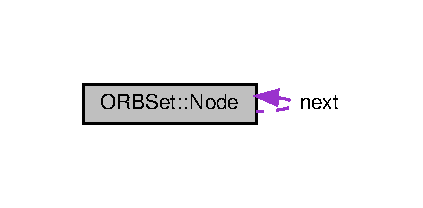
\includegraphics[width=203pt]{df/dc1/structORBSet_1_1Node__coll__graph}
\end{center}
\end{figure}
\subsection*{Public Attributes}
\begin{DoxyCompactItemize}
\item 
\mbox{\Hypertarget{structORBSet_1_1Node_a30880197d04672d02efd8e1b840e0d9d}\label{structORBSet_1_1Node_a30880197d04672d02efd8e1b840e0d9d}} 
struct \hyperlink{structORBSet_1_1Node}{Node} $\ast$ {\bfseries next}
\item 
\mbox{\Hypertarget{structORBSet_1_1Node_aae0249065130dcbb2f1b785dfc06751b}\label{structORBSet_1_1Node_aae0249065130dcbb2f1b785dfc06751b}} 
const char $\ast$ {\bfseries node\+\_\+name}
\end{DoxyCompactItemize}


\subsection{Detailed Description}


Definition at line 42 of file O\+R\+B\+Set.\+hpp.



The documentation for this struct was generated from the following file\+:\begin{DoxyCompactItemize}
\item 
/home/andressanchez/\+Escritorio/\+G\+I\+T/project\+\_\+template/src/modules/u\+O\+R\+B/O\+R\+B\+Set.\+hpp\end{DoxyCompactItemize}

\hypertarget{structuORB_1_1orb__advertdata}{}\section{u\+O\+RB\+:\+:orb\+\_\+advertdata Struct Reference}
\label{structuORB_1_1orb__advertdata}\index{u\+O\+R\+B\+::orb\+\_\+advertdata@{u\+O\+R\+B\+::orb\+\_\+advertdata}}


Collaboration diagram for u\+O\+RB\+:\+:orb\+\_\+advertdata\+:\nopagebreak
\begin{figure}[H]
\begin{center}
\leavevmode
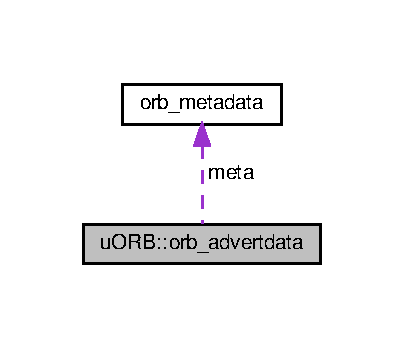
\includegraphics[width=194pt]{d7/d7a/structuORB_1_1orb__advertdata__coll__graph}
\end{center}
\end{figure}
\subsection*{Public Attributes}
\begin{DoxyCompactItemize}
\item 
\mbox{\Hypertarget{structuORB_1_1orb__advertdata_ae64bf6fa26c5e4527b10915d99a120ef}\label{structuORB_1_1orb__advertdata_ae64bf6fa26c5e4527b10915d99a120ef}} 
const struct \hyperlink{structorb__metadata}{orb\+\_\+metadata} $\ast$ {\bfseries meta}
\item 
\mbox{\Hypertarget{structuORB_1_1orb__advertdata_a9c25a2ad60208f58430b18b5d3d28e7e}\label{structuORB_1_1orb__advertdata_a9c25a2ad60208f58430b18b5d3d28e7e}} 
int $\ast$ {\bfseries instance}
\end{DoxyCompactItemize}


\subsection{Detailed Description}


Definition at line 47 of file u\+O\+R\+B\+Common.\+hpp.



The documentation for this struct was generated from the following file\+:\begin{DoxyCompactItemize}
\item 
/home/andressanchez/\+Escritorio/\+G\+I\+T/project\+\_\+template/src/modules/u\+O\+R\+B/u\+O\+R\+B\+Common.\+hpp\end{DoxyCompactItemize}

\hypertarget{structorb__metadata}{}\section{orb\+\_\+metadata Struct Reference}
\label{structorb__metadata}\index{orb\+\_\+metadata@{orb\+\_\+metadata}}


{\ttfamily \#include $<$u\+O\+R\+B.\+h$>$}

\subsection*{Public Attributes}
\begin{DoxyCompactItemize}
\item 
const char $\ast$ \hyperlink{structorb__metadata_a54d1751f24aa0c1f24934c6712811e58}{o\+\_\+name}
\item 
const uint16\+\_\+t \hyperlink{structorb__metadata_a400a86fe707613e881b620cde7888b74}{o\+\_\+size}
\item 
const uint16\+\_\+t \hyperlink{structorb__metadata_a5a3abec9c79b3b46e97bf0c4cf9c68dd}{o\+\_\+size\+\_\+no\+\_\+padding}
\item 
const char $\ast$ \hyperlink{structorb__metadata_a0eca59345d0097080daec156bb7a9c1f}{o\+\_\+fields}
\item 
uint8\+\_\+t \hyperlink{structorb__metadata_a9f5cae5c486a015774b7accc62ca040e}{o\+\_\+id}
\end{DoxyCompactItemize}


\subsection{Detailed Description}
Object metadata. 

Definition at line 54 of file u\+O\+R\+B.\+h.



\subsection{Member Data Documentation}
\mbox{\Hypertarget{structorb__metadata_a0eca59345d0097080daec156bb7a9c1f}\label{structorb__metadata_a0eca59345d0097080daec156bb7a9c1f}} 
\index{orb\+\_\+metadata@{orb\+\_\+metadata}!o\+\_\+fields@{o\+\_\+fields}}
\index{o\+\_\+fields@{o\+\_\+fields}!orb\+\_\+metadata@{orb\+\_\+metadata}}
\subsubsection{\texorpdfstring{o\+\_\+fields}{o\_fields}}
{\footnotesize\ttfamily const char$\ast$ orb\+\_\+metadata\+::o\+\_\+fields}

semicolon separated list of fields (with type) 

Definition at line 58 of file u\+O\+R\+B.\+h.

\mbox{\Hypertarget{structorb__metadata_a9f5cae5c486a015774b7accc62ca040e}\label{structorb__metadata_a9f5cae5c486a015774b7accc62ca040e}} 
\index{orb\+\_\+metadata@{orb\+\_\+metadata}!o\+\_\+id@{o\+\_\+id}}
\index{o\+\_\+id@{o\+\_\+id}!orb\+\_\+metadata@{orb\+\_\+metadata}}
\subsubsection{\texorpdfstring{o\+\_\+id}{o\_id}}
{\footnotesize\ttfamily uint8\+\_\+t orb\+\_\+metadata\+::o\+\_\+id}

O\+R\+B\+\_\+\+ID enum 

Definition at line 59 of file u\+O\+R\+B.\+h.

\mbox{\Hypertarget{structorb__metadata_a54d1751f24aa0c1f24934c6712811e58}\label{structorb__metadata_a54d1751f24aa0c1f24934c6712811e58}} 
\index{orb\+\_\+metadata@{orb\+\_\+metadata}!o\+\_\+name@{o\+\_\+name}}
\index{o\+\_\+name@{o\+\_\+name}!orb\+\_\+metadata@{orb\+\_\+metadata}}
\subsubsection{\texorpdfstring{o\+\_\+name}{o\_name}}
{\footnotesize\ttfamily const char$\ast$ orb\+\_\+metadata\+::o\+\_\+name}

unique object name 

Definition at line 55 of file u\+O\+R\+B.\+h.

\mbox{\Hypertarget{structorb__metadata_a400a86fe707613e881b620cde7888b74}\label{structorb__metadata_a400a86fe707613e881b620cde7888b74}} 
\index{orb\+\_\+metadata@{orb\+\_\+metadata}!o\+\_\+size@{o\+\_\+size}}
\index{o\+\_\+size@{o\+\_\+size}!orb\+\_\+metadata@{orb\+\_\+metadata}}
\subsubsection{\texorpdfstring{o\+\_\+size}{o\_size}}
{\footnotesize\ttfamily const uint16\+\_\+t orb\+\_\+metadata\+::o\+\_\+size}

object size 

Definition at line 56 of file u\+O\+R\+B.\+h.

\mbox{\Hypertarget{structorb__metadata_a5a3abec9c79b3b46e97bf0c4cf9c68dd}\label{structorb__metadata_a5a3abec9c79b3b46e97bf0c4cf9c68dd}} 
\index{orb\+\_\+metadata@{orb\+\_\+metadata}!o\+\_\+size\+\_\+no\+\_\+padding@{o\+\_\+size\+\_\+no\+\_\+padding}}
\index{o\+\_\+size\+\_\+no\+\_\+padding@{o\+\_\+size\+\_\+no\+\_\+padding}!orb\+\_\+metadata@{orb\+\_\+metadata}}
\subsubsection{\texorpdfstring{o\+\_\+size\+\_\+no\+\_\+padding}{o\_size\_no\_padding}}
{\footnotesize\ttfamily const uint16\+\_\+t orb\+\_\+metadata\+::o\+\_\+size\+\_\+no\+\_\+padding}

object size w/o padding at the end (for logger) 

Definition at line 57 of file u\+O\+R\+B.\+h.



The documentation for this struct was generated from the following file\+:\begin{DoxyCompactItemize}
\item 
/home/andressanchez/\+Escritorio/\+G\+I\+T/project\+\_\+template/src/modules/u\+O\+R\+B/\hyperlink{uORB_8h}{u\+O\+R\+B.\+h}\end{DoxyCompactItemize}

\hypertarget{structorb__test__s}{}\section{orb\+\_\+test\+\_\+s Struct Reference}
\label{structorb__test__s}\index{orb\+\_\+test\+\_\+s@{orb\+\_\+test\+\_\+s}}
\subsection*{Public Attributes}
\begin{DoxyCompactItemize}
\item 
\mbox{\Hypertarget{structorb__test__s_a5def43d9b1795f9f5cc367f091d01c10}\label{structorb__test__s_a5def43d9b1795f9f5cc367f091d01c10}} 
uint64\+\_\+t {\bfseries timestamp}
\item 
\mbox{\Hypertarget{structorb__test__s_a7ca7d4e30e3c1d5512222ea29d192dd1}\label{structorb__test__s_a7ca7d4e30e3c1d5512222ea29d192dd1}} 
int32\+\_\+t {\bfseries val}
\item 
\mbox{\Hypertarget{structorb__test__s_a43eb923766090656a5e6a5e4624359d9}\label{structorb__test__s_a43eb923766090656a5e6a5e4624359d9}} 
uint8\+\_\+t {\bfseries \+\_\+padding0} \mbox{[}4\mbox{]}
\end{DoxyCompactItemize}


\subsection{Detailed Description}


Definition at line 51 of file orb\+\_\+test.\+h.



The documentation for this struct was generated from the following file\+:\begin{DoxyCompactItemize}
\item 
/home/andressanchez/\+Escritorio/\+G\+I\+T/project\+\_\+template/src/modules/u\+O\+R\+B/topics/orb\+\_\+test.\+h\end{DoxyCompactItemize}

\hypertarget{classORBSet}{}\section{O\+R\+B\+Set Class Reference}
\label{classORBSet}\index{O\+R\+B\+Set@{O\+R\+B\+Set}}
\subsection*{Classes}
\begin{DoxyCompactItemize}
\item 
struct \hyperlink{structORBSet_1_1Node}{Node}
\end{DoxyCompactItemize}
\subsection*{Public Member Functions}
\begin{DoxyCompactItemize}
\item 
\mbox{\Hypertarget{classORBSet_a3a2605821e231411fed3e8ab0ad8a611}\label{classORBSet_a3a2605821e231411fed3e8ab0ad8a611}} 
void {\bfseries insert} (const char $\ast$node\+\_\+name)
\item 
\mbox{\Hypertarget{classORBSet_ac903d6b53015b957f557d4c42773a77c}\label{classORBSet_ac903d6b53015b957f557d4c42773a77c}} 
bool {\bfseries find} (const char $\ast$node\+\_\+name)
\item 
\mbox{\Hypertarget{classORBSet_a2d3d5339d7db8b52e168301df480929a}\label{classORBSet_a2d3d5339d7db8b52e168301df480929a}} 
bool {\bfseries erase} (const char $\ast$node\+\_\+name)
\end{DoxyCompactItemize}


\subsection{Detailed Description}


Definition at line 39 of file O\+R\+B\+Set.\+hpp.



The documentation for this class was generated from the following file\+:\begin{DoxyCompactItemize}
\item 
/home/andressanchez/\+Escritorio/\+G\+I\+T/project\+\_\+template/src/modules/u\+O\+R\+B/O\+R\+B\+Set.\+hpp\end{DoxyCompactItemize}

\hypertarget{classuORB_1_1Publication}{}\section{u\+O\+RB\+:\+:Publication$<$ T, O\+R\+B\+\_\+\+Q\+S\+I\+ZE $>$ Class Template Reference}
\label{classuORB_1_1Publication}\index{u\+O\+R\+B\+::\+Publication$<$ T, O\+R\+B\+\_\+\+Q\+S\+I\+Z\+E $>$@{u\+O\+R\+B\+::\+Publication$<$ T, O\+R\+B\+\_\+\+Q\+S\+I\+Z\+E $>$}}


{\ttfamily \#include $<$Publication.\+hpp$>$}



Inheritance diagram for u\+O\+RB\+:\+:Publication$<$ T, O\+R\+B\+\_\+\+Q\+S\+I\+ZE $>$\+:\nopagebreak
\begin{figure}[H]
\begin{center}
\leavevmode
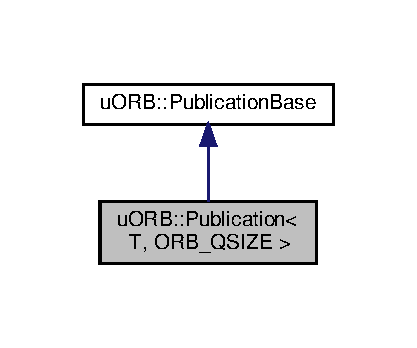
\includegraphics[width=200pt]{d0/d46/classuORB_1_1Publication__inherit__graph}
\end{center}
\end{figure}


Collaboration diagram for u\+O\+RB\+:\+:Publication$<$ T, O\+R\+B\+\_\+\+Q\+S\+I\+ZE $>$\+:\nopagebreak
\begin{figure}[H]
\begin{center}
\leavevmode
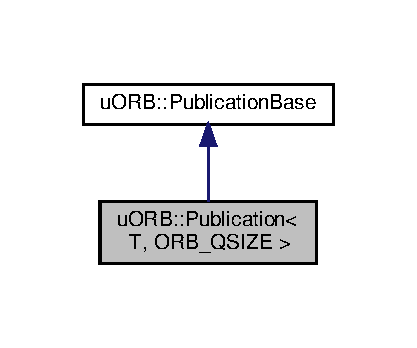
\includegraphics[width=200pt]{dd/d69/classuORB_1_1Publication__coll__graph}
\end{center}
\end{figure}
\subsection*{Public Member Functions}
\begin{DoxyCompactItemize}
\item 
\hyperlink{classuORB_1_1Publication_a420de66872fa317bed932a5e54698323}{Publication} (\hyperlink{uORB_8h_a96af5434ec1acdf24287bd7851b0413f}{O\+R\+B\+\_\+\+ID} id)
\item 
\mbox{\Hypertarget{classuORB_1_1Publication_a0bcd30a2e20035adcd7b053e8e4dbe4b}\label{classuORB_1_1Publication_a0bcd30a2e20035adcd7b053e8e4dbe4b}} 
{\bfseries Publication} (const \hyperlink{structorb__metadata}{orb\+\_\+metadata} $\ast$meta)
\item 
\mbox{\Hypertarget{classuORB_1_1Publication_a4af3fc463148dec3ddfb597824cc8c37}\label{classuORB_1_1Publication_a4af3fc463148dec3ddfb597824cc8c37}} 
bool {\bfseries advertise} ()
\item 
bool \hyperlink{classuORB_1_1Publication_a1c4a9ef046f8b0c1ade8a226e36f2892}{publish} (const T \&data)
\end{DoxyCompactItemize}
\subsection*{Additional Inherited Members}


\subsection{Detailed Description}
\subsubsection*{template$<$typename T, uint8\+\_\+t O\+R\+B\+\_\+\+Q\+S\+I\+ZE = 1$>$\newline
class u\+O\+R\+B\+::\+Publication$<$ T, O\+R\+B\+\_\+\+Q\+S\+I\+Z\+E $>$}

u\+O\+RB publication wrapper class 

Definition at line 80 of file Publication.\+hpp.



\subsection{Constructor \& Destructor Documentation}
\mbox{\Hypertarget{classuORB_1_1Publication_a420de66872fa317bed932a5e54698323}\label{classuORB_1_1Publication_a420de66872fa317bed932a5e54698323}} 
\index{u\+O\+R\+B\+::\+Publication@{u\+O\+R\+B\+::\+Publication}!Publication@{Publication}}
\index{Publication@{Publication}!u\+O\+R\+B\+::\+Publication@{u\+O\+R\+B\+::\+Publication}}
\subsubsection{\texorpdfstring{Publication()}{Publication()}}
{\footnotesize\ttfamily template$<$typename T, uint8\+\_\+t O\+R\+B\+\_\+\+Q\+S\+I\+ZE = 1$>$ \\
\hyperlink{classuORB_1_1Publication}{u\+O\+R\+B\+::\+Publication}$<$ T, O\+R\+B\+\_\+\+Q\+S\+I\+ZE $>$\+::\hyperlink{classuORB_1_1Publication}{Publication} (\begin{DoxyParamCaption}\item[{\hyperlink{uORB_8h_a96af5434ec1acdf24287bd7851b0413f}{O\+R\+B\+\_\+\+ID}}]{id }\end{DoxyParamCaption})\hspace{0.3cm}{\ttfamily [inline]}}

Constructor


\begin{DoxyParams}{Parameters}
{\em meta} & The u\+O\+RB metadata (usually from the \hyperlink{uORB_8h_a96af5434ec1acdf24287bd7851b0413f}{O\+R\+B\+\_\+\+I\+D()} macro) for the topic. \\
\hline
\end{DoxyParams}


Definition at line 89 of file Publication.\+hpp.


\begin{DoxyCode}
89 : PublicationBase(\textcolor{keywordtype}{id}) \{\}
\end{DoxyCode}


\subsection{Member Function Documentation}
\mbox{\Hypertarget{classuORB_1_1Publication_a1c4a9ef046f8b0c1ade8a226e36f2892}\label{classuORB_1_1Publication_a1c4a9ef046f8b0c1ade8a226e36f2892}} 
\index{u\+O\+R\+B\+::\+Publication@{u\+O\+R\+B\+::\+Publication}!publish@{publish}}
\index{publish@{publish}!u\+O\+R\+B\+::\+Publication@{u\+O\+R\+B\+::\+Publication}}
\subsubsection{\texorpdfstring{publish()}{publish()}}
{\footnotesize\ttfamily template$<$typename T, uint8\+\_\+t O\+R\+B\+\_\+\+Q\+S\+I\+ZE = 1$>$ \\
bool \hyperlink{classuORB_1_1Publication}{u\+O\+R\+B\+::\+Publication}$<$ T, O\+R\+B\+\_\+\+Q\+S\+I\+ZE $>$\+::publish (\begin{DoxyParamCaption}\item[{const T \&}]{data }\end{DoxyParamCaption})\hspace{0.3cm}{\ttfamily [inline]}}

Publish the struct 
\begin{DoxyParams}{Parameters}
{\em data} & The u\+O\+RB message struct we are updating. \\
\hline
\end{DoxyParams}


Definition at line 105 of file Publication.\+hpp.


\begin{DoxyCode}
106     \{
107         \textcolor{keywordflow}{if} (!advertised()) \{
108             advertise();
109         \}
110 
111         \textcolor{keywordflow}{return} (\hyperlink{classuORB_1_1DeviceNode_ae715517a1f3a2f361e37d061b59a4560}{uORB::DeviceNode::publish}(get\_topic(), \_handle, &data) == 0);
112     \}
\end{DoxyCode}


The documentation for this class was generated from the following file\+:\begin{DoxyCompactItemize}
\item 
/home/andressanchez/\+Escritorio/\+G\+I\+T/project\+\_\+template/src/modules/u\+O\+R\+B/\hyperlink{Publication_8hpp}{Publication.\+hpp}\end{DoxyCompactItemize}

\hypertarget{classuORB_1_1PublicationBase}{}\section{u\+O\+RB\+:\+:Publication\+Base Class Reference}
\label{classuORB_1_1PublicationBase}\index{u\+O\+R\+B\+::\+Publication\+Base@{u\+O\+R\+B\+::\+Publication\+Base}}


Inheritance diagram for u\+O\+RB\+:\+:Publication\+Base\+:\nopagebreak
\begin{figure}[H]
\begin{center}
\leavevmode
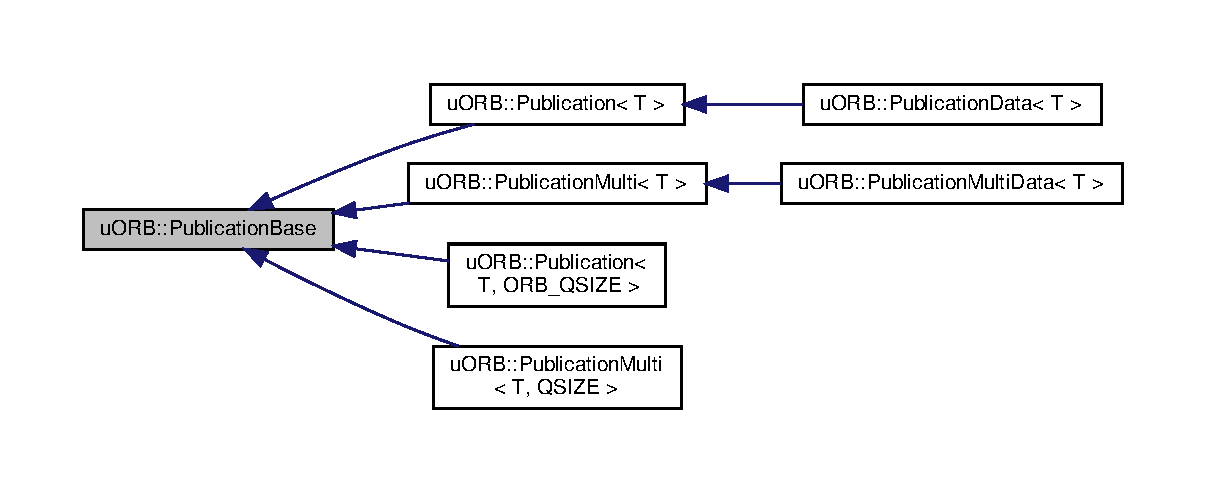
\includegraphics[width=350pt]{d0/d95/classuORB_1_1PublicationBase__inherit__graph}
\end{center}
\end{figure}
\subsection*{Public Member Functions}
\begin{DoxyCompactItemize}
\item 
\mbox{\Hypertarget{classuORB_1_1PublicationBase_a7b21359765206fde43a3700c3e8179e4}\label{classuORB_1_1PublicationBase_a7b21359765206fde43a3700c3e8179e4}} 
bool {\bfseries advertised} () const
\item 
\mbox{\Hypertarget{classuORB_1_1PublicationBase_a8d5bafb4b89d6894176b0a57d2f69310}\label{classuORB_1_1PublicationBase_a8d5bafb4b89d6894176b0a57d2f69310}} 
bool {\bfseries unadvertise} ()
\item 
\mbox{\Hypertarget{classuORB_1_1PublicationBase_a106832b4ccbf1efe88acd7d32ab0ea7e}\label{classuORB_1_1PublicationBase_a106832b4ccbf1efe88acd7d32ab0ea7e}} 
\hyperlink{structorb__metadata}{orb\+\_\+id\+\_\+t} {\bfseries get\+\_\+topic} () const
\end{DoxyCompactItemize}
\subsection*{Protected Member Functions}
\begin{DoxyCompactItemize}
\item 
\mbox{\Hypertarget{classuORB_1_1PublicationBase_a8d0ea2cadf61656b9d6168377d5dd7d6}\label{classuORB_1_1PublicationBase_a8d0ea2cadf61656b9d6168377d5dd7d6}} 
{\bfseries Publication\+Base} (\hyperlink{uORB_8h_a96af5434ec1acdf24287bd7851b0413f}{O\+R\+B\+\_\+\+ID} id)
\end{DoxyCompactItemize}
\subsection*{Protected Attributes}
\begin{DoxyCompactItemize}
\item 
\mbox{\Hypertarget{classuORB_1_1PublicationBase_a4254d929704949ce6ef55e1b9a9d3037}\label{classuORB_1_1PublicationBase_a4254d929704949ce6ef55e1b9a9d3037}} 
\hyperlink{uORB_8h_a8d0cfa5f9ea6427a37057d6cea6dd990}{orb\+\_\+advert\+\_\+t} {\bfseries \+\_\+handle} \{nullptr\}
\item 
\mbox{\Hypertarget{classuORB_1_1PublicationBase_a72f822f0ac8d4853c15c71de9d27f03a}\label{classuORB_1_1PublicationBase_a72f822f0ac8d4853c15c71de9d27f03a}} 
const \hyperlink{uORB_8h_a96af5434ec1acdf24287bd7851b0413f}{O\+R\+B\+\_\+\+ID} {\bfseries \+\_\+orb\+\_\+id}
\end{DoxyCompactItemize}


\subsection{Detailed Description}


Definition at line 48 of file Publication.\+hpp.



The documentation for this class was generated from the following file\+:\begin{DoxyCompactItemize}
\item 
/home/andressanchez/\+Escritorio/\+G\+I\+T/project\+\_\+template/src/modules/u\+O\+R\+B/\hyperlink{Publication_8hpp}{Publication.\+hpp}\end{DoxyCompactItemize}

\hypertarget{classuORB_1_1PublicationData}{}\section{u\+O\+RB\+:\+:Publication\+Data$<$ T $>$ Class Template Reference}
\label{classuORB_1_1PublicationData}\index{u\+O\+R\+B\+::\+Publication\+Data$<$ T $>$@{u\+O\+R\+B\+::\+Publication\+Data$<$ T $>$}}


{\ttfamily \#include $<$Publication.\+hpp$>$}



Inheritance diagram for u\+O\+RB\+:\+:Publication\+Data$<$ T $>$\+:\nopagebreak
\begin{figure}[H]
\begin{center}
\leavevmode
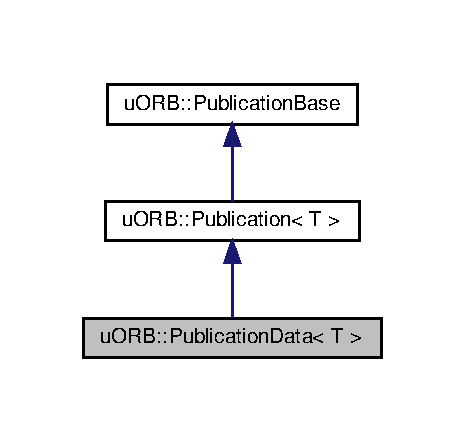
\includegraphics[width=223pt]{dd/db7/classuORB_1_1PublicationData__inherit__graph}
\end{center}
\end{figure}


Collaboration diagram for u\+O\+RB\+:\+:Publication\+Data$<$ T $>$\+:\nopagebreak
\begin{figure}[H]
\begin{center}
\leavevmode
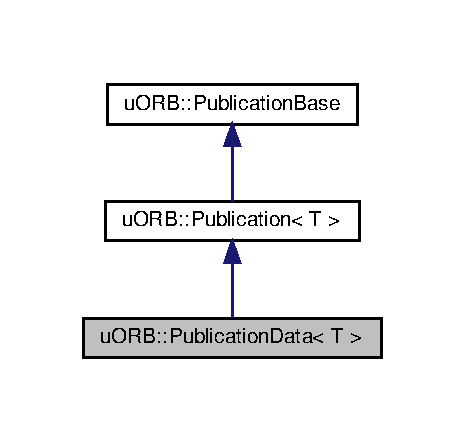
\includegraphics[width=223pt]{d1/dca/classuORB_1_1PublicationData__coll__graph}
\end{center}
\end{figure}
\subsection*{Public Member Functions}
\begin{DoxyCompactItemize}
\item 
\hyperlink{classuORB_1_1PublicationData_a666841966b36304506549f012b65da49}{Publication\+Data} (\hyperlink{uORB_8h_a96af5434ec1acdf24287bd7851b0413f}{O\+R\+B\+\_\+\+ID} id)
\item 
\mbox{\Hypertarget{classuORB_1_1PublicationData_ae93ef2f5bc7e52a1c59f5b421134ee39}\label{classuORB_1_1PublicationData_ae93ef2f5bc7e52a1c59f5b421134ee39}} 
{\bfseries Publication\+Data} (const \hyperlink{structorb__metadata}{orb\+\_\+metadata} $\ast$meta)
\item 
\mbox{\Hypertarget{classuORB_1_1PublicationData_a713677de3cb15c58e29294f2009075ba}\label{classuORB_1_1PublicationData_a713677de3cb15c58e29294f2009075ba}} 
T \& {\bfseries get} ()
\item 
\mbox{\Hypertarget{classuORB_1_1PublicationData_a1e334845584e67bf990554245f73cb7a}\label{classuORB_1_1PublicationData_a1e334845584e67bf990554245f73cb7a}} 
void {\bfseries set} (const T \&data)
\item 
\mbox{\Hypertarget{classuORB_1_1PublicationData_a59a09d55fc1196a57c39bc7b36ee997d}\label{classuORB_1_1PublicationData_a59a09d55fc1196a57c39bc7b36ee997d}} 
bool {\bfseries update} ()
\item 
\mbox{\Hypertarget{classuORB_1_1PublicationData_aa081268dd303e6210a2fa62688b89333}\label{classuORB_1_1PublicationData_aa081268dd303e6210a2fa62688b89333}} 
bool {\bfseries update} (const T \&data)
\end{DoxyCompactItemize}
\subsection*{Additional Inherited Members}


\subsection{Detailed Description}
\subsubsection*{template$<$typename T$>$\newline
class u\+O\+R\+B\+::\+Publication\+Data$<$ T $>$}

The publication class with data embedded. 

Definition at line 119 of file Publication.\+hpp.



\subsection{Constructor \& Destructor Documentation}
\mbox{\Hypertarget{classuORB_1_1PublicationData_a666841966b36304506549f012b65da49}\label{classuORB_1_1PublicationData_a666841966b36304506549f012b65da49}} 
\index{u\+O\+R\+B\+::\+Publication\+Data@{u\+O\+R\+B\+::\+Publication\+Data}!Publication\+Data@{Publication\+Data}}
\index{Publication\+Data@{Publication\+Data}!u\+O\+R\+B\+::\+Publication\+Data@{u\+O\+R\+B\+::\+Publication\+Data}}
\subsubsection{\texorpdfstring{Publication\+Data()}{PublicationData()}}
{\footnotesize\ttfamily template$<$typename T $>$ \\
\hyperlink{classuORB_1_1PublicationData}{u\+O\+R\+B\+::\+Publication\+Data}$<$ T $>$\+::\hyperlink{classuORB_1_1PublicationData}{Publication\+Data} (\begin{DoxyParamCaption}\item[{\hyperlink{uORB_8h_a96af5434ec1acdf24287bd7851b0413f}{O\+R\+B\+\_\+\+ID}}]{id }\end{DoxyParamCaption})\hspace{0.3cm}{\ttfamily [inline]}}

Constructor


\begin{DoxyParams}{Parameters}
{\em meta} & The u\+O\+RB metadata (usually from the \hyperlink{uORB_8h_a96af5434ec1acdf24287bd7851b0413f}{O\+R\+B\+\_\+\+I\+D()} macro) for the topic. \\
\hline
\end{DoxyParams}


Definition at line 127 of file Publication.\+hpp.


\begin{DoxyCode}
127 : Publication<T>(id) \{\}
\end{DoxyCode}


The documentation for this class was generated from the following file\+:\begin{DoxyCompactItemize}
\item 
/home/andressanchez/\+Escritorio/\+G\+I\+T/project\+\_\+template/src/modules/u\+O\+R\+B/\hyperlink{Publication_8hpp}{Publication.\+hpp}\end{DoxyCompactItemize}

\hypertarget{classuORB_1_1PublicationMulti}{}\section{u\+O\+RB\+:\+:Publication\+Multi$<$ T, Q\+S\+I\+ZE $>$ Class Template Reference}
\label{classuORB_1_1PublicationMulti}\index{u\+O\+R\+B\+::\+Publication\+Multi$<$ T, Q\+S\+I\+Z\+E $>$@{u\+O\+R\+B\+::\+Publication\+Multi$<$ T, Q\+S\+I\+Z\+E $>$}}


{\ttfamily \#include $<$Publication\+Multi.\+hpp$>$}



Inheritance diagram for u\+O\+RB\+:\+:Publication\+Multi$<$ T, Q\+S\+I\+ZE $>$\+:\nopagebreak
\begin{figure}[H]
\begin{center}
\leavevmode
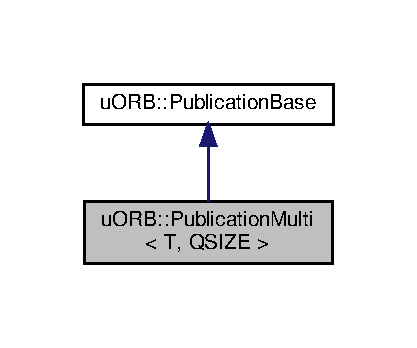
\includegraphics[width=200pt]{d7/df4/classuORB_1_1PublicationMulti__inherit__graph}
\end{center}
\end{figure}


Collaboration diagram for u\+O\+RB\+:\+:Publication\+Multi$<$ T, Q\+S\+I\+ZE $>$\+:\nopagebreak
\begin{figure}[H]
\begin{center}
\leavevmode
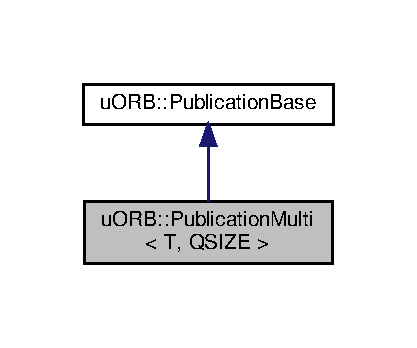
\includegraphics[width=200pt]{d0/d47/classuORB_1_1PublicationMulti__coll__graph}
\end{center}
\end{figure}
\subsection*{Public Member Functions}
\begin{DoxyCompactItemize}
\item 
\hyperlink{classuORB_1_1PublicationMulti_a012ffe3988cb69d32bc9a9e2807843a5}{Publication\+Multi} (\hyperlink{uORB_8h_a96af5434ec1acdf24287bd7851b0413f}{O\+R\+B\+\_\+\+ID} id)
\item 
\mbox{\Hypertarget{classuORB_1_1PublicationMulti_ad035712d9637183bf85ff41f7f00521a}\label{classuORB_1_1PublicationMulti_ad035712d9637183bf85ff41f7f00521a}} 
{\bfseries Publication\+Multi} (const \hyperlink{structorb__metadata}{orb\+\_\+metadata} $\ast$meta)
\item 
\mbox{\Hypertarget{classuORB_1_1PublicationMulti_a663a534a770585e9fe6025d393a80651}\label{classuORB_1_1PublicationMulti_a663a534a770585e9fe6025d393a80651}} 
bool {\bfseries advertise} ()
\item 
bool \hyperlink{classuORB_1_1PublicationMulti_a98dd47e770678acb5bc7489a90cd9cdd}{publish} (const T \&data)
\end{DoxyCompactItemize}
\subsection*{Additional Inherited Members}


\subsection{Detailed Description}
\subsubsection*{template$<$typename T, uint8\+\_\+t Q\+S\+I\+ZE = 1$>$\newline
class u\+O\+R\+B\+::\+Publication\+Multi$<$ T, Q\+S\+I\+Z\+E $>$}

Base publication multi wrapper class 

Definition at line 51 of file Publication\+Multi.\+hpp.



\subsection{Constructor \& Destructor Documentation}
\mbox{\Hypertarget{classuORB_1_1PublicationMulti_a012ffe3988cb69d32bc9a9e2807843a5}\label{classuORB_1_1PublicationMulti_a012ffe3988cb69d32bc9a9e2807843a5}} 
\index{u\+O\+R\+B\+::\+Publication\+Multi@{u\+O\+R\+B\+::\+Publication\+Multi}!Publication\+Multi@{Publication\+Multi}}
\index{Publication\+Multi@{Publication\+Multi}!u\+O\+R\+B\+::\+Publication\+Multi@{u\+O\+R\+B\+::\+Publication\+Multi}}
\subsubsection{\texorpdfstring{Publication\+Multi()}{PublicationMulti()}}
{\footnotesize\ttfamily template$<$typename T, uint8\+\_\+t Q\+S\+I\+ZE = 1$>$ \\
\hyperlink{classuORB_1_1PublicationMulti}{u\+O\+R\+B\+::\+Publication\+Multi}$<$ T, Q\+S\+I\+ZE $>$\+::\hyperlink{classuORB_1_1PublicationMulti}{Publication\+Multi} (\begin{DoxyParamCaption}\item[{\hyperlink{uORB_8h_a96af5434ec1acdf24287bd7851b0413f}{O\+R\+B\+\_\+\+ID}}]{id }\end{DoxyParamCaption})\hspace{0.3cm}{\ttfamily [inline]}}

Constructor


\begin{DoxyParams}{Parameters}
{\em meta} & The u\+O\+RB metadata (usually from the \hyperlink{uORB_8h_a96af5434ec1acdf24287bd7851b0413f}{O\+R\+B\+\_\+\+I\+D()} macro) for the topic. \\
\hline
\end{DoxyParams}


Definition at line 60 of file Publication\+Multi.\+hpp.


\begin{DoxyCode}
60                                 :
61         PublicationBase(\textcolor{keywordtype}{id})
62     \{\}
\end{DoxyCode}


\subsection{Member Function Documentation}
\mbox{\Hypertarget{classuORB_1_1PublicationMulti_a98dd47e770678acb5bc7489a90cd9cdd}\label{classuORB_1_1PublicationMulti_a98dd47e770678acb5bc7489a90cd9cdd}} 
\index{u\+O\+R\+B\+::\+Publication\+Multi@{u\+O\+R\+B\+::\+Publication\+Multi}!publish@{publish}}
\index{publish@{publish}!u\+O\+R\+B\+::\+Publication\+Multi@{u\+O\+R\+B\+::\+Publication\+Multi}}
\subsubsection{\texorpdfstring{publish()}{publish()}}
{\footnotesize\ttfamily template$<$typename T, uint8\+\_\+t Q\+S\+I\+ZE = 1$>$ \\
bool \hyperlink{classuORB_1_1PublicationMulti}{u\+O\+R\+B\+::\+Publication\+Multi}$<$ T, Q\+S\+I\+ZE $>$\+::publish (\begin{DoxyParamCaption}\item[{const T \&}]{data }\end{DoxyParamCaption})\hspace{0.3cm}{\ttfamily [inline]}}

Publish the struct 
\begin{DoxyParams}{Parameters}
{\em data} & The u\+O\+RB message struct we are updating. \\
\hline
\end{DoxyParams}


Definition at line 82 of file Publication\+Multi.\+hpp.


\begin{DoxyCode}
83     \{
84         \textcolor{keywordflow}{if} (!advertised()) \{
85             advertise();
86         \}
87 
88         \textcolor{keywordflow}{return} (\hyperlink{uORB_8cpp_af7a143a80b6b04689a3a4890ce8df4ae}{orb\_publish}(get\_topic(), \_handle, &data) == 0);
89     \}
\end{DoxyCode}


The documentation for this class was generated from the following file\+:\begin{DoxyCompactItemize}
\item 
/home/andressanchez/\+Escritorio/\+G\+I\+T/project\+\_\+template/src/modules/u\+O\+R\+B/Publication\+Multi.\+hpp\end{DoxyCompactItemize}

\hypertarget{classuORB_1_1PublicationMultiData}{}\section{u\+O\+RB\+:\+:Publication\+Multi\+Data$<$ T $>$ Class Template Reference}
\label{classuORB_1_1PublicationMultiData}\index{u\+O\+R\+B\+::\+Publication\+Multi\+Data$<$ T $>$@{u\+O\+R\+B\+::\+Publication\+Multi\+Data$<$ T $>$}}


{\ttfamily \#include $<$Publication\+Multi.\+hpp$>$}



Inheritance diagram for u\+O\+RB\+:\+:Publication\+Multi\+Data$<$ T $>$\+:\nopagebreak
\begin{figure}[H]
\begin{center}
\leavevmode
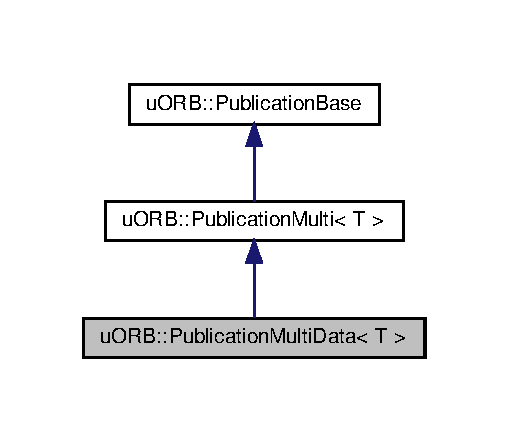
\includegraphics[width=244pt]{d6/da8/classuORB_1_1PublicationMultiData__inherit__graph}
\end{center}
\end{figure}


Collaboration diagram for u\+O\+RB\+:\+:Publication\+Multi\+Data$<$ T $>$\+:\nopagebreak
\begin{figure}[H]
\begin{center}
\leavevmode
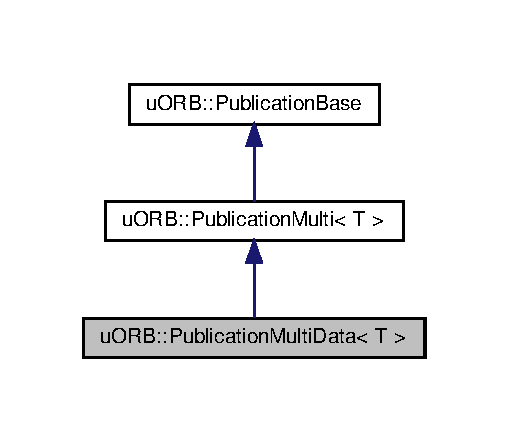
\includegraphics[width=244pt]{d5/d2e/classuORB_1_1PublicationMultiData__coll__graph}
\end{center}
\end{figure}
\subsection*{Public Member Functions}
\begin{DoxyCompactItemize}
\item 
\hyperlink{classuORB_1_1PublicationMultiData_ae7c681d67caa481cb875aa1427dd73ec}{Publication\+Multi\+Data} (\hyperlink{uORB_8h_a96af5434ec1acdf24287bd7851b0413f}{O\+R\+B\+\_\+\+ID} id)
\item 
\mbox{\Hypertarget{classuORB_1_1PublicationMultiData_ae0297ff38a92fe596256ca1f3969beea}\label{classuORB_1_1PublicationMultiData_ae0297ff38a92fe596256ca1f3969beea}} 
{\bfseries Publication\+Multi\+Data} (const \hyperlink{structorb__metadata}{orb\+\_\+metadata} $\ast$meta)
\item 
\mbox{\Hypertarget{classuORB_1_1PublicationMultiData_ad34053c0417701f6951d21e5b6618b34}\label{classuORB_1_1PublicationMultiData_ad34053c0417701f6951d21e5b6618b34}} 
T \& {\bfseries get} ()
\item 
\mbox{\Hypertarget{classuORB_1_1PublicationMultiData_a7739de2d33219a5328494c4a95799725}\label{classuORB_1_1PublicationMultiData_a7739de2d33219a5328494c4a95799725}} 
void {\bfseries set} (const T \&data)
\item 
\mbox{\Hypertarget{classuORB_1_1PublicationMultiData_a42d8c47f80211bac32dfdf1792609a83}\label{classuORB_1_1PublicationMultiData_a42d8c47f80211bac32dfdf1792609a83}} 
bool {\bfseries update} ()
\item 
\mbox{\Hypertarget{classuORB_1_1PublicationMultiData_a91f2f51e9d1b34bdec7a1db63b47ea77}\label{classuORB_1_1PublicationMultiData_a91f2f51e9d1b34bdec7a1db63b47ea77}} 
bool {\bfseries update} (const T \&data)
\end{DoxyCompactItemize}
\subsection*{Additional Inherited Members}


\subsection{Detailed Description}
\subsubsection*{template$<$typename T$>$\newline
class u\+O\+R\+B\+::\+Publication\+Multi\+Data$<$ T $>$}

The publication multi class with data embedded. 

Definition at line 96 of file Publication\+Multi.\+hpp.



\subsection{Constructor \& Destructor Documentation}
\mbox{\Hypertarget{classuORB_1_1PublicationMultiData_ae7c681d67caa481cb875aa1427dd73ec}\label{classuORB_1_1PublicationMultiData_ae7c681d67caa481cb875aa1427dd73ec}} 
\index{u\+O\+R\+B\+::\+Publication\+Multi\+Data@{u\+O\+R\+B\+::\+Publication\+Multi\+Data}!Publication\+Multi\+Data@{Publication\+Multi\+Data}}
\index{Publication\+Multi\+Data@{Publication\+Multi\+Data}!u\+O\+R\+B\+::\+Publication\+Multi\+Data@{u\+O\+R\+B\+::\+Publication\+Multi\+Data}}
\subsubsection{\texorpdfstring{Publication\+Multi\+Data()}{PublicationMultiData()}}
{\footnotesize\ttfamily template$<$typename T $>$ \\
\hyperlink{classuORB_1_1PublicationMultiData}{u\+O\+R\+B\+::\+Publication\+Multi\+Data}$<$ T $>$\+::\hyperlink{classuORB_1_1PublicationMultiData}{Publication\+Multi\+Data} (\begin{DoxyParamCaption}\item[{\hyperlink{uORB_8h_a96af5434ec1acdf24287bd7851b0413f}{O\+R\+B\+\_\+\+ID}}]{id }\end{DoxyParamCaption})\hspace{0.3cm}{\ttfamily [inline]}}

Constructor


\begin{DoxyParams}{Parameters}
{\em meta} & The u\+O\+RB metadata (usually from the \hyperlink{uORB_8h_a96af5434ec1acdf24287bd7851b0413f}{O\+R\+B\+\_\+\+I\+D()} macro) for the topic. \\
\hline
\end{DoxyParams}


Definition at line 104 of file Publication\+Multi.\+hpp.


\begin{DoxyCode}
104 : PublicationMulti<T>(id) \{\}
\end{DoxyCode}


The documentation for this class was generated from the following file\+:\begin{DoxyCompactItemize}
\item 
/home/andressanchez/\+Escritorio/\+G\+I\+T/project\+\_\+template/src/modules/u\+O\+R\+B/Publication\+Multi.\+hpp\end{DoxyCompactItemize}

\hypertarget{classuORB_1_1Subscription}{}\section{u\+O\+RB\+:\+:Subscription Class Reference}
\label{classuORB_1_1Subscription}\index{u\+O\+R\+B\+::\+Subscription@{u\+O\+R\+B\+::\+Subscription}}


Inheritance diagram for u\+O\+RB\+:\+:Subscription\+:\nopagebreak
\begin{figure}[H]
\begin{center}
\leavevmode
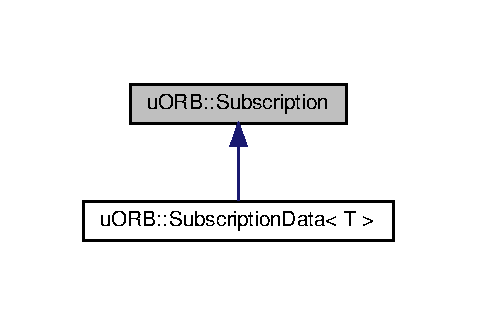
\includegraphics[width=229pt]{db/d59/classuORB_1_1Subscription__inherit__graph}
\end{center}
\end{figure}


Collaboration diagram for u\+O\+RB\+:\+:Subscription\+:\nopagebreak
\begin{figure}[H]
\begin{center}
\leavevmode
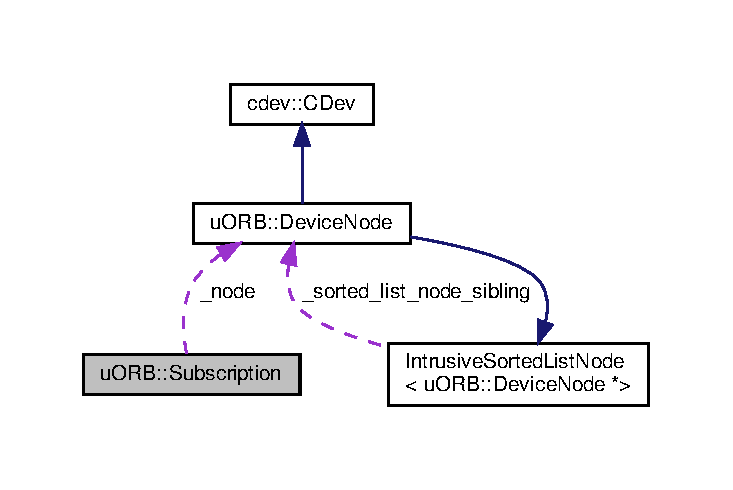
\includegraphics[width=350pt]{db/d78/classuORB_1_1Subscription__coll__graph}
\end{center}
\end{figure}
\subsection*{Public Member Functions}
\begin{DoxyCompactItemize}
\item 
\hyperlink{classuORB_1_1Subscription_a6afd37f8aa13bc3ffeafd29b7a3d434f}{Subscription} (\hyperlink{uORB_8h_a96af5434ec1acdf24287bd7851b0413f}{O\+R\+B\+\_\+\+ID} id, uint8\+\_\+t instance=0)
\item 
\hyperlink{classuORB_1_1Subscription_a8851d25ec7fc746ed71214cb65500006}{Subscription} (const \hyperlink{structorb__metadata}{orb\+\_\+metadata} $\ast$meta, uint8\+\_\+t instance=0)
\item 
bool \hyperlink{classuORB_1_1Subscription_acb0fbd4b56d5e3c8edca15206e110223}{subscribe} ()
\item 
\mbox{\Hypertarget{classuORB_1_1Subscription_a4228366c28dfaed084710f13e48934be}\label{classuORB_1_1Subscription_a4228366c28dfaed084710f13e48934be}} 
void {\bfseries unsubscribe} ()
\item 
\mbox{\Hypertarget{classuORB_1_1Subscription_af4675ee1722445e07e50d1a984b8d8c0}\label{classuORB_1_1Subscription_af4675ee1722445e07e50d1a984b8d8c0}} 
bool {\bfseries valid} () const
\item 
\mbox{\Hypertarget{classuORB_1_1Subscription_a9c16cd791d522e477bfafbbc09729bc2}\label{classuORB_1_1Subscription_a9c16cd791d522e477bfafbbc09729bc2}} 
bool {\bfseries advertised} ()
\item 
bool \hyperlink{classuORB_1_1Subscription_a788d1848a46abe88a093be9a1f7cb2ca}{updated} ()
\item 
bool \hyperlink{classuORB_1_1Subscription_a2376542413f8b31c20bcbfc1a11b13ea}{update} (void $\ast$dst)
\item 
bool \hyperlink{classuORB_1_1Subscription_a17a37eb5624b409379db434400de4582}{copy} (void $\ast$dst)
\item 
bool \hyperlink{classuORB_1_1Subscription_a47a32a02ea909df267542d4b4ef99115}{Change\+Instance} (uint8\+\_\+t instance)
\item 
\mbox{\Hypertarget{classuORB_1_1Subscription_ab0c5d9ec0df8e62343413302d6e97fa0}\label{classuORB_1_1Subscription_ab0c5d9ec0df8e62343413302d6e97fa0}} 
uint8\+\_\+t {\bfseries get\+\_\+instance} () const
\item 
\mbox{\Hypertarget{classuORB_1_1Subscription_ad7aaf2211cb1a5ec96cdfda9cabac174}\label{classuORB_1_1Subscription_ad7aaf2211cb1a5ec96cdfda9cabac174}} 
unsigned {\bfseries get\+\_\+last\+\_\+generation} () const
\item 
\mbox{\Hypertarget{classuORB_1_1Subscription_a447b0f0a9e4745f3dcc2bcdf2540d940}\label{classuORB_1_1Subscription_a447b0f0a9e4745f3dcc2bcdf2540d940}} 
\hyperlink{structorb__metadata}{orb\+\_\+id\+\_\+t} {\bfseries get\+\_\+topic} () const
\end{DoxyCompactItemize}
\subsection*{Protected Member Functions}
\begin{DoxyCompactItemize}
\item 
\mbox{\Hypertarget{classuORB_1_1Subscription_acfefc1961589348321e83851139512ce}\label{classuORB_1_1Subscription_acfefc1961589348321e83851139512ce}} 
\hyperlink{classuORB_1_1DeviceNode}{Device\+Node} $\ast$ {\bfseries get\+\_\+node} ()
\end{DoxyCompactItemize}
\subsection*{Protected Attributes}
\begin{DoxyCompactItemize}
\item 
\mbox{\Hypertarget{classuORB_1_1Subscription_a0d3a0c177af4386b4f3d306a1b995dbc}\label{classuORB_1_1Subscription_a0d3a0c177af4386b4f3d306a1b995dbc}} 
\hyperlink{classuORB_1_1DeviceNode}{Device\+Node} $\ast$ {\bfseries \+\_\+node} \{nullptr\}
\item 
unsigned \hyperlink{classuORB_1_1Subscription_a994ab022fce2eb1c47b62444d9c5cca9}{\+\_\+last\+\_\+generation} \{0\}
\item 
\mbox{\Hypertarget{classuORB_1_1Subscription_ab117a8b8e0b79caaf37847e1f208fa7b}\label{classuORB_1_1Subscription_ab117a8b8e0b79caaf37847e1f208fa7b}} 
\hyperlink{uORB_8h_a96af5434ec1acdf24287bd7851b0413f}{O\+R\+B\+\_\+\+ID} {\bfseries \+\_\+orb\+\_\+id} \{O\+R\+B\+\_\+\+I\+D\+::\+I\+N\+V\+A\+L\+ID\}
\item 
\mbox{\Hypertarget{classuORB_1_1Subscription_a96128476244a201e40b2ffe1ae2fee07}\label{classuORB_1_1Subscription_a96128476244a201e40b2ffe1ae2fee07}} 
uint8\+\_\+t {\bfseries \+\_\+instance} \{0\}
\end{DoxyCompactItemize}
\subsection*{Friends}
\begin{DoxyCompactItemize}
\item 
\mbox{\Hypertarget{classuORB_1_1Subscription_a140e44567b16af0d25b0c7f04f2839c7}\label{classuORB_1_1Subscription_a140e44567b16af0d25b0c7f04f2839c7}} 
class {\bfseries Subscription\+Callback}
\item 
\mbox{\Hypertarget{classuORB_1_1Subscription_a1a53a356246a3520bc25153445812f1b}\label{classuORB_1_1Subscription_a1a53a356246a3520bc25153445812f1b}} 
class {\bfseries Subscription\+Callback\+Work\+Item}
\end{DoxyCompactItemize}


\subsection{Detailed Description}


Definition at line 58 of file Subscription.\+hpp.



\subsection{Constructor \& Destructor Documentation}
\mbox{\Hypertarget{classuORB_1_1Subscription_a6afd37f8aa13bc3ffeafd29b7a3d434f}\label{classuORB_1_1Subscription_a6afd37f8aa13bc3ffeafd29b7a3d434f}} 
\index{u\+O\+R\+B\+::\+Subscription@{u\+O\+R\+B\+::\+Subscription}!Subscription@{Subscription}}
\index{Subscription@{Subscription}!u\+O\+R\+B\+::\+Subscription@{u\+O\+R\+B\+::\+Subscription}}
\subsubsection{\texorpdfstring{Subscription()}{Subscription()}\hspace{0.1cm}{\footnotesize\ttfamily [1/2]}}
{\footnotesize\ttfamily u\+O\+R\+B\+::\+Subscription\+::\+Subscription (\begin{DoxyParamCaption}\item[{\hyperlink{uORB_8h_a96af5434ec1acdf24287bd7851b0413f}{O\+R\+B\+\_\+\+ID}}]{id,  }\item[{uint8\+\_\+t}]{instance = {\ttfamily 0} }\end{DoxyParamCaption})\hspace{0.3cm}{\ttfamily [inline]}}

Constructor


\begin{DoxyParams}{Parameters}
{\em id} & The u\+O\+RB O\+R\+B\+\_\+\+ID enum for the topic. \\
\hline
{\em instance} & The instance for multi sub. \\
\hline
\end{DoxyParams}


Definition at line 68 of file Subscription.\+hpp.


\begin{DoxyCode}
68                                                   :
69         \_orb\_id(\textcolor{keywordtype}{id}),
70         \_instance(instance)
71     \{
72         \hyperlink{classuORB_1_1Subscription_acb0fbd4b56d5e3c8edca15206e110223}{subscribe}();
73     \}
\end{DoxyCode}
\mbox{\Hypertarget{classuORB_1_1Subscription_a8851d25ec7fc746ed71214cb65500006}\label{classuORB_1_1Subscription_a8851d25ec7fc746ed71214cb65500006}} 
\index{u\+O\+R\+B\+::\+Subscription@{u\+O\+R\+B\+::\+Subscription}!Subscription@{Subscription}}
\index{Subscription@{Subscription}!u\+O\+R\+B\+::\+Subscription@{u\+O\+R\+B\+::\+Subscription}}
\subsubsection{\texorpdfstring{Subscription()}{Subscription()}\hspace{0.1cm}{\footnotesize\ttfamily [2/2]}}
{\footnotesize\ttfamily u\+O\+R\+B\+::\+Subscription\+::\+Subscription (\begin{DoxyParamCaption}\item[{const \hyperlink{structorb__metadata}{orb\+\_\+metadata} $\ast$}]{meta,  }\item[{uint8\+\_\+t}]{instance = {\ttfamily 0} }\end{DoxyParamCaption})\hspace{0.3cm}{\ttfamily [inline]}}

Constructor


\begin{DoxyParams}{Parameters}
{\em meta} & The u\+O\+RB metadata (usually from the \hyperlink{uORB_8h_a96af5434ec1acdf24287bd7851b0413f}{O\+R\+B\+\_\+\+I\+D()} macro) for the topic. \\
\hline
{\em instance} & The instance for multi sub. \\
\hline
\end{DoxyParams}


Definition at line 81 of file Subscription.\+hpp.


\begin{DoxyCode}
81                                                                  :
82         \_orb\_id((meta == \textcolor{keyword}{nullptr}) ? ORB\_ID::INVALID : static\_cast<ORB\_ID>(meta->
      \hyperlink{structorb__metadata_a9f5cae5c486a015774b7accc62ca040e}{o\_id})),
83         \_instance(instance)
84     \{
85         \hyperlink{classuORB_1_1Subscription_acb0fbd4b56d5e3c8edca15206e110223}{subscribe}();
86     \}
\end{DoxyCode}


\subsection{Member Function Documentation}
\mbox{\Hypertarget{classuORB_1_1Subscription_a47a32a02ea909df267542d4b4ef99115}\label{classuORB_1_1Subscription_a47a32a02ea909df267542d4b4ef99115}} 
\index{u\+O\+R\+B\+::\+Subscription@{u\+O\+R\+B\+::\+Subscription}!Change\+Instance@{Change\+Instance}}
\index{Change\+Instance@{Change\+Instance}!u\+O\+R\+B\+::\+Subscription@{u\+O\+R\+B\+::\+Subscription}}
\subsubsection{\texorpdfstring{Change\+Instance()}{ChangeInstance()}}
{\footnotesize\ttfamily bool u\+O\+R\+B\+::\+Subscription\+::\+Change\+Instance (\begin{DoxyParamCaption}\item[{uint8\+\_\+t}]{instance }\end{DoxyParamCaption})}

Change subscription instance 
\begin{DoxyParams}{Parameters}
{\em instance} & The new multi-\/\+Subscription instance \\
\hline
\end{DoxyParams}


Definition at line 93 of file Subscription.\+cpp.


\begin{DoxyCode}
94 \{
95     \textcolor{keywordflow}{if} (instance != \_instance) \{
96         DeviceMaster *device\_master = \hyperlink{classuORB_1_1Manager_a9d829b3ea49d16d03c2fa37ef2bb24a5}{uORB::Manager::get\_instance}()->
      \hyperlink{classuORB_1_1Manager_a083331e24ac4f99ac11a0aab1b1681b4}{get\_device\_master}();
97 
98         \textcolor{keywordflow}{if} (device\_master != \textcolor{keyword}{nullptr}) \{
99             \textcolor{keywordflow}{if} (!device\_master->deviceNodeExists(\_orb\_id, \_instance)) \{
100                 \textcolor{keywordflow}{return} \textcolor{keyword}{false};
101             \}
102 
103             \textcolor{comment}{// if desired new instance exists, unsubscribe from current}
104             unsubscribe();
105             \_instance = instance;
106             \hyperlink{classuORB_1_1Subscription_acb0fbd4b56d5e3c8edca15206e110223}{subscribe}();
107             \textcolor{keywordflow}{return} \textcolor{keyword}{true};
108         \}
109 
110     \} \textcolor{keywordflow}{else} \{
111         \textcolor{comment}{// already on desired index}
112         \textcolor{keywordflow}{return} \textcolor{keyword}{true};
113     \}
114 
115     \textcolor{keywordflow}{return} \textcolor{keyword}{false};
116 \}
\end{DoxyCode}
\mbox{\Hypertarget{classuORB_1_1Subscription_a17a37eb5624b409379db434400de4582}\label{classuORB_1_1Subscription_a17a37eb5624b409379db434400de4582}} 
\index{u\+O\+R\+B\+::\+Subscription@{u\+O\+R\+B\+::\+Subscription}!copy@{copy}}
\index{copy@{copy}!u\+O\+R\+B\+::\+Subscription@{u\+O\+R\+B\+::\+Subscription}}
\subsubsection{\texorpdfstring{copy()}{copy()}}
{\footnotesize\ttfamily bool u\+O\+R\+B\+::\+Subscription\+::copy (\begin{DoxyParamCaption}\item[{void $\ast$}]{dst }\end{DoxyParamCaption})\hspace{0.3cm}{\ttfamily [inline]}}

Copy the struct 
\begin{DoxyParams}{Parameters}
{\em dst} & The u\+O\+RB message struct we are updating. \\
\hline
\end{DoxyParams}


Definition at line 129 of file Subscription.\+hpp.


\begin{DoxyCode}
129 \{ \textcolor{keywordflow}{return} advertised() && \_node->\hyperlink{classuORB_1_1DeviceNode_a89d9a792e1e38e04c65baba20f29d780}{copy}(dst, \hyperlink{classuORB_1_1Subscription_a994ab022fce2eb1c47b62444d9c5cca9}{\_last\_generation}); \}
\end{DoxyCode}
\mbox{\Hypertarget{classuORB_1_1Subscription_acb0fbd4b56d5e3c8edca15206e110223}\label{classuORB_1_1Subscription_acb0fbd4b56d5e3c8edca15206e110223}} 
\index{u\+O\+R\+B\+::\+Subscription@{u\+O\+R\+B\+::\+Subscription}!subscribe@{subscribe}}
\index{subscribe@{subscribe}!u\+O\+R\+B\+::\+Subscription@{u\+O\+R\+B\+::\+Subscription}}
\subsubsection{\texorpdfstring{subscribe()}{subscribe()}}
{\footnotesize\ttfamily bool u\+O\+R\+B\+::\+Subscription\+::subscribe (\begin{DoxyParamCaption}{ }\end{DoxyParamCaption})}

(curr\+\_\+gen$<$(unsigned)\+\_\+node-\/$>$get\+\_\+queue\+\_\+size())?(unsigned)\+\_\+node-\/$>$get\+\_\+queue\+\_\+size()\+:curr\+\_\+gen; 

Definition at line 46 of file Subscription.\+cpp.


\begin{DoxyCode}
47 \{
48     \textcolor{comment}{// check if already subscribed}
49     \textcolor{keywordflow}{if} (\_node != \textcolor{keyword}{nullptr}) \{
50         \textcolor{keywordflow}{return} \textcolor{keyword}{true};
51     \}
52 
53     \textcolor{keywordflow}{if} (\_orb\_id != ORB\_ID::INVALID) \{
54 
55         DeviceMaster *device\_master = \hyperlink{classuORB_1_1Manager_a9d829b3ea49d16d03c2fa37ef2bb24a5}{uORB::Manager::get\_instance}()->
      \hyperlink{classuORB_1_1Manager_a083331e24ac4f99ac11a0aab1b1681b4}{get\_device\_master}();
56 
57         \textcolor{keywordflow}{if} (device\_master != \textcolor{keyword}{nullptr}) \{
58 
59             \textcolor{keywordflow}{if} (!device\_master->deviceNodeExists(\_orb\_id, \_instance)) \{
60                 \textcolor{keywordflow}{return} \textcolor{keyword}{false};
61             \}
62 
63             \hyperlink{classuORB_1_1DeviceNode}{uORB::DeviceNode} *node = device\_master->getDeviceNode(get\_topic(), \_instance);
64 
65             \textcolor{keywordflow}{if} (node != \textcolor{keyword}{nullptr}) \{
66                 \_node = node;
67                 \_node->\hyperlink{classuORB_1_1DeviceNode_abb03278ff4ddd2a50e0f2996e856f2cc}{add\_internal\_subscriber}();
68 
69                 \textcolor{keyword}{const} \textcolor{keywordtype}{unsigned} curr\_gen = \_node->published\_message\_count();
70 
71                 \textcolor{comment}{// If there were any previous publications allow the subscriber to read them}
73 \textcolor{comment}{}                \hyperlink{classuORB_1_1Subscription_a994ab022fce2eb1c47b62444d9c5cca9}{\_last\_generation} = curr\_gen - !(curr\_gen<(unsigned)\_node->get\_queue\_size())
      ?(\textcolor{keywordtype}{unsigned})\_node->get\_queue\_size():curr\_gen;
74 
75                 \textcolor{keywordflow}{return} \textcolor{keyword}{true};
76             \}
77         \}
78     \}
79 
80     \textcolor{keywordflow}{return} \textcolor{keyword}{false};
81 \}
\end{DoxyCode}
\mbox{\Hypertarget{classuORB_1_1Subscription_a2376542413f8b31c20bcbfc1a11b13ea}\label{classuORB_1_1Subscription_a2376542413f8b31c20bcbfc1a11b13ea}} 
\index{u\+O\+R\+B\+::\+Subscription@{u\+O\+R\+B\+::\+Subscription}!update@{update}}
\index{update@{update}!u\+O\+R\+B\+::\+Subscription@{u\+O\+R\+B\+::\+Subscription}}
\subsubsection{\texorpdfstring{update()}{update()}}
{\footnotesize\ttfamily bool u\+O\+R\+B\+::\+Subscription\+::update (\begin{DoxyParamCaption}\item[{void $\ast$}]{dst }\end{DoxyParamCaption})\hspace{0.3cm}{\ttfamily [inline]}}

Update the struct 
\begin{DoxyParams}{Parameters}
{\em dst} & The u\+O\+RB message struct we are updating. \\
\hline
\end{DoxyParams}


Definition at line 123 of file Subscription.\+hpp.


\begin{DoxyCode}
123 \{ \textcolor{keywordflow}{return} \hyperlink{classuORB_1_1Subscription_a788d1848a46abe88a093be9a1f7cb2ca}{updated}() && \_node->\hyperlink{classuORB_1_1DeviceNode_a89d9a792e1e38e04c65baba20f29d780}{copy}(dst, \hyperlink{classuORB_1_1Subscription_a994ab022fce2eb1c47b62444d9c5cca9}{\_last\_generation}); \}
\end{DoxyCode}
\mbox{\Hypertarget{classuORB_1_1Subscription_a788d1848a46abe88a093be9a1f7cb2ca}\label{classuORB_1_1Subscription_a788d1848a46abe88a093be9a1f7cb2ca}} 
\index{u\+O\+R\+B\+::\+Subscription@{u\+O\+R\+B\+::\+Subscription}!updated@{updated}}
\index{updated@{updated}!u\+O\+R\+B\+::\+Subscription@{u\+O\+R\+B\+::\+Subscription}}
\subsubsection{\texorpdfstring{updated()}{updated()}}
{\footnotesize\ttfamily bool u\+O\+R\+B\+::\+Subscription\+::updated (\begin{DoxyParamCaption}{ }\end{DoxyParamCaption})\hspace{0.3cm}{\ttfamily [inline]}}

Check if there is a new update. 

Definition at line 117 of file Subscription.\+hpp.


\begin{DoxyCode}
117 \{ \textcolor{keywordflow}{return} advertised() && (\_node->published\_message\_count() != \hyperlink{classuORB_1_1Subscription_a994ab022fce2eb1c47b62444d9c5cca9}{\_last\_generation}); \}
\end{DoxyCode}


\subsection{Member Data Documentation}
\mbox{\Hypertarget{classuORB_1_1Subscription_a994ab022fce2eb1c47b62444d9c5cca9}\label{classuORB_1_1Subscription_a994ab022fce2eb1c47b62444d9c5cca9}} 
\index{u\+O\+R\+B\+::\+Subscription@{u\+O\+R\+B\+::\+Subscription}!\+\_\+last\+\_\+generation@{\+\_\+last\+\_\+generation}}
\index{\+\_\+last\+\_\+generation@{\+\_\+last\+\_\+generation}!u\+O\+R\+B\+::\+Subscription@{u\+O\+R\+B\+::\+Subscription}}
\subsubsection{\texorpdfstring{\+\_\+last\+\_\+generation}{\_last\_generation}}
{\footnotesize\ttfamily unsigned u\+O\+R\+B\+::\+Subscription\+::\+\_\+last\+\_\+generation \{0\}\hspace{0.3cm}{\ttfamily [protected]}}

last generation the subscriber has seen 

Definition at line 150 of file Subscription.\+hpp.



The documentation for this class was generated from the following files\+:\begin{DoxyCompactItemize}
\item 
/home/andressanchez/\+Escritorio/\+G\+I\+T/project\+\_\+template/src/modules/u\+O\+R\+B/\hyperlink{Subscription_8hpp}{Subscription.\+hpp}\item 
/home/andressanchez/\+Escritorio/\+G\+I\+T/project\+\_\+template/src/modules/u\+O\+R\+B/\hyperlink{Subscription_8cpp}{Subscription.\+cpp}\end{DoxyCompactItemize}

\hypertarget{classuORB_1_1SubscriptionBlocking}{}\section{u\+O\+RB\+:\+:Subscription\+Blocking$<$ T $>$ Class Template Reference}
\label{classuORB_1_1SubscriptionBlocking}\index{u\+O\+R\+B\+::\+Subscription\+Blocking$<$ T $>$@{u\+O\+R\+B\+::\+Subscription\+Blocking$<$ T $>$}}


Inheritance diagram for u\+O\+RB\+:\+:Subscription\+Blocking$<$ T $>$\+:\nopagebreak
\begin{figure}[H]
\begin{center}
\leavevmode
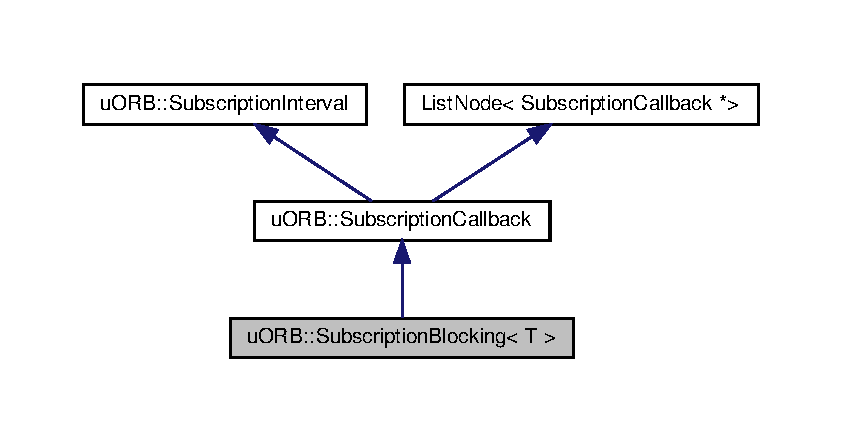
\includegraphics[width=350pt]{df/d8b/classuORB_1_1SubscriptionBlocking__inherit__graph}
\end{center}
\end{figure}


Collaboration diagram for u\+O\+RB\+:\+:Subscription\+Blocking$<$ T $>$\+:\nopagebreak
\begin{figure}[H]
\begin{center}
\leavevmode
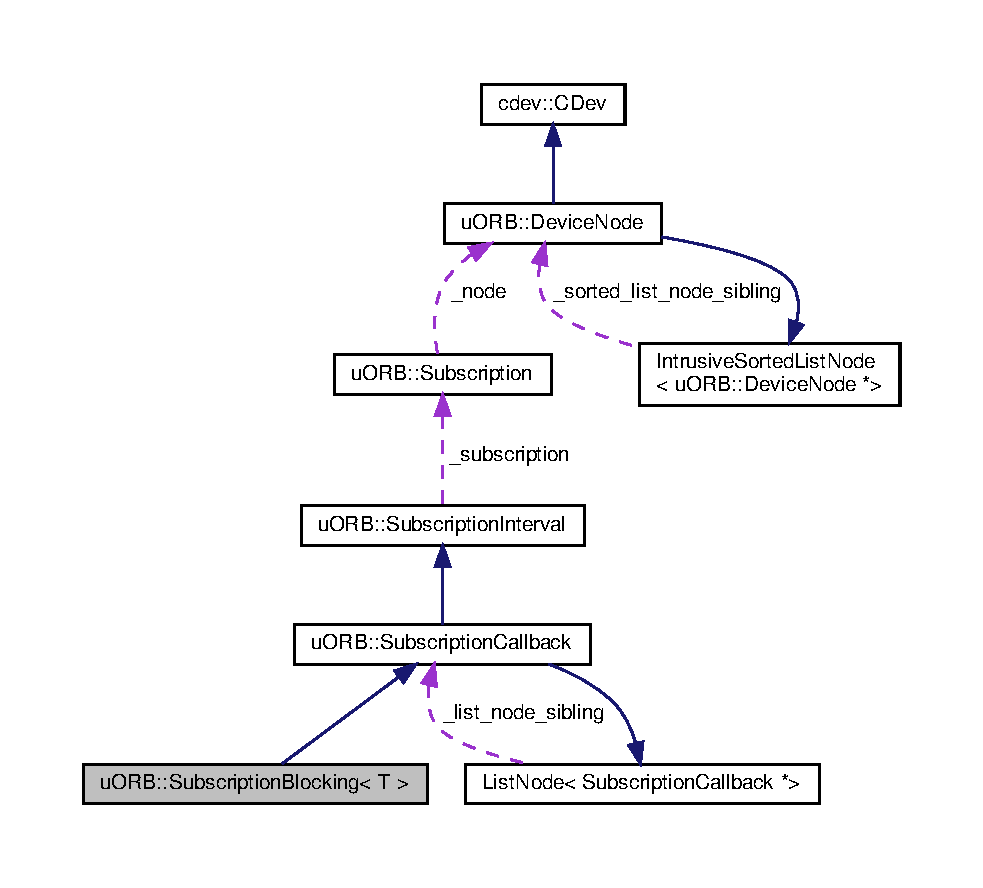
\includegraphics[width=350pt]{d4/d7d/classuORB_1_1SubscriptionBlocking__coll__graph}
\end{center}
\end{figure}
\subsection*{Public Member Functions}
\begin{DoxyCompactItemize}
\item 
\hyperlink{classuORB_1_1SubscriptionBlocking_a112e322e269b8d7c577f1dde3b5e8393}{Subscription\+Blocking} (const \hyperlink{structorb__metadata}{orb\+\_\+metadata} $\ast$meta, uint32\+\_\+t interval\+\_\+us=0, uint8\+\_\+t instance=0)
\item 
\mbox{\Hypertarget{classuORB_1_1SubscriptionBlocking_ab151303fb1a35645cc86570031991a58}\label{classuORB_1_1SubscriptionBlocking_ab151303fb1a35645cc86570031991a58}} 
void {\bfseries call} () override
\item 
bool \hyperlink{classuORB_1_1SubscriptionBlocking_af6a2f560b911949ed11eabc0cfad7874}{updated\+Blocking} (uint32\+\_\+t timeout\+\_\+us=0)
\item 
bool \hyperlink{classuORB_1_1SubscriptionBlocking_ab1e6e657ca5ebbaf53fde6204109350d}{update\+Blocking} (T \&data, uint32\+\_\+t timeout\+\_\+us=0)
\end{DoxyCompactItemize}
\subsection*{Additional Inherited Members}


\subsection{Detailed Description}
\subsubsection*{template$<$typename T$>$\newline
class u\+O\+R\+B\+::\+Subscription\+Blocking$<$ T $>$}



Definition at line 47 of file Subscription\+Blocking.\+hpp.



\subsection{Constructor \& Destructor Documentation}
\mbox{\Hypertarget{classuORB_1_1SubscriptionBlocking_a112e322e269b8d7c577f1dde3b5e8393}\label{classuORB_1_1SubscriptionBlocking_a112e322e269b8d7c577f1dde3b5e8393}} 
\index{u\+O\+R\+B\+::\+Subscription\+Blocking@{u\+O\+R\+B\+::\+Subscription\+Blocking}!Subscription\+Blocking@{Subscription\+Blocking}}
\index{Subscription\+Blocking@{Subscription\+Blocking}!u\+O\+R\+B\+::\+Subscription\+Blocking@{u\+O\+R\+B\+::\+Subscription\+Blocking}}
\subsubsection{\texorpdfstring{Subscription\+Blocking()}{SubscriptionBlocking()}}
{\footnotesize\ttfamily template$<$typename T $>$ \\
\hyperlink{classuORB_1_1SubscriptionBlocking}{u\+O\+R\+B\+::\+Subscription\+Blocking}$<$ T $>$\+::\hyperlink{classuORB_1_1SubscriptionBlocking}{Subscription\+Blocking} (\begin{DoxyParamCaption}\item[{const \hyperlink{structorb__metadata}{orb\+\_\+metadata} $\ast$}]{meta,  }\item[{uint32\+\_\+t}]{interval\+\_\+us = {\ttfamily 0},  }\item[{uint8\+\_\+t}]{instance = {\ttfamily 0} }\end{DoxyParamCaption})\hspace{0.3cm}{\ttfamily [inline]}}

Constructor


\begin{DoxyParams}{Parameters}
{\em meta} & The u\+O\+RB metadata (usually from the \hyperlink{uORB_8h_a96af5434ec1acdf24287bd7851b0413f}{O\+R\+B\+\_\+\+I\+D()} macro) for the topic. \\
\hline
{\em interval\+\_\+us} & The requested maximum update interval in microseconds. \\
\hline
{\em instance} & The instance for multi sub. \\
\hline
\end{DoxyParams}


Definition at line 57 of file Subscription\+Blocking.\+hpp.


\begin{DoxyCode}
57                                                                                                    :
58         \hyperlink{classuORB_1_1SubscriptionCallback_acc7373f302eb194d01734aedab1db772}{SubscriptionCallback}(meta, interval\_us, instance)
59     \{
60         \textcolor{comment}{// pthread\_mutexattr\_init}
61         pthread\_mutexattr\_t attr;
62         \textcolor{keywordtype}{int} ret\_attr\_init = pthread\_mutexattr\_init(&attr);
63 
64         \textcolor{keywordflow}{if} (ret\_attr\_init != 0) \{
65             \textcolor{comment}{//PX4\_ERR("pthread\_mutexattr\_init failed, status=%d", ret\_attr\_init);}
66         \}
67 
68 \textcolor{preprocessor}{#if defined(PTHREAD\_PRIO\_NONE)}
69         \textcolor{comment}{// pthread\_mutexattr\_settype}
70         \textcolor{comment}{//  PTHREAD\_PRIO\_NONE not available on cygwin}
71         \textcolor{keywordtype}{int} ret\_mutexattr\_settype = pthread\_mutexattr\_settype(&attr, PTHREAD\_PRIO\_NONE);
72 
73         \textcolor{keywordflow}{if} (ret\_mutexattr\_settype != 0) \{
74             \textcolor{comment}{//PX4\_ERR("pthread\_mutexattr\_settype failed, status=%d", ret\_mutexattr\_settype);}
75         \}
76 
77 \textcolor{preprocessor}{#endif // PTHREAD\_PRIO\_NONE}
78 
79         \textcolor{comment}{// pthread\_mutex\_init}
80         \textcolor{keywordtype}{int} ret\_mutex\_init = pthread\_mutex\_init(&\_mutex, &attr);
81 
82         \textcolor{keywordflow}{if} (ret\_mutex\_init != 0) \{
83             \textcolor{comment}{//PX4\_ERR("pthread\_mutex\_init failed, status=%d", ret\_mutex\_init);}
84         \}
85     \}
\end{DoxyCode}


\subsection{Member Function Documentation}
\mbox{\Hypertarget{classuORB_1_1SubscriptionBlocking_ab1e6e657ca5ebbaf53fde6204109350d}\label{classuORB_1_1SubscriptionBlocking_ab1e6e657ca5ebbaf53fde6204109350d}} 
\index{u\+O\+R\+B\+::\+Subscription\+Blocking@{u\+O\+R\+B\+::\+Subscription\+Blocking}!update\+Blocking@{update\+Blocking}}
\index{update\+Blocking@{update\+Blocking}!u\+O\+R\+B\+::\+Subscription\+Blocking@{u\+O\+R\+B\+::\+Subscription\+Blocking}}
\subsubsection{\texorpdfstring{update\+Blocking()}{updateBlocking()}}
{\footnotesize\ttfamily template$<$typename T $>$ \\
bool \hyperlink{classuORB_1_1SubscriptionBlocking}{u\+O\+R\+B\+::\+Subscription\+Blocking}$<$ T $>$\+::update\+Blocking (\begin{DoxyParamCaption}\item[{T \&}]{data,  }\item[{uint32\+\_\+t}]{timeout\+\_\+us = {\ttfamily 0} }\end{DoxyParamCaption})\hspace{0.3cm}{\ttfamily [inline]}}

Copy the struct if updated. 
\begin{DoxyParams}{Parameters}
{\em data} & The data reference where the struct will be copied. \\
\hline
{\em timeout\+\_\+us} & The requested timeout in microseconds, or 0 to wait indefinitely.\\
\hline
\end{DoxyParams}
\begin{DoxyReturn}{Returns}
true only if topic was updated and copied successfully. 
\end{DoxyReturn}


Definition at line 157 of file Subscription\+Blocking.\+hpp.


\begin{DoxyCode}
158     \{
159         \textcolor{keywordflow}{if} (\hyperlink{classuORB_1_1SubscriptionBlocking_af6a2f560b911949ed11eabc0cfad7874}{updatedBlocking}(timeout\_us)) \{
160             \textcolor{keywordflow}{return} \hyperlink{classuORB_1_1SubscriptionInterval_a25125ed09772665d3b4b4e6978fb3e1c}{copy}(&data);
161         \}
162 
163         \textcolor{keywordflow}{return} \textcolor{keyword}{false};
164     \}
\end{DoxyCode}
\mbox{\Hypertarget{classuORB_1_1SubscriptionBlocking_af6a2f560b911949ed11eabc0cfad7874}\label{classuORB_1_1SubscriptionBlocking_af6a2f560b911949ed11eabc0cfad7874}} 
\index{u\+O\+R\+B\+::\+Subscription\+Blocking@{u\+O\+R\+B\+::\+Subscription\+Blocking}!updated\+Blocking@{updated\+Blocking}}
\index{updated\+Blocking@{updated\+Blocking}!u\+O\+R\+B\+::\+Subscription\+Blocking@{u\+O\+R\+B\+::\+Subscription\+Blocking}}
\subsubsection{\texorpdfstring{updated\+Blocking()}{updatedBlocking()}}
{\footnotesize\ttfamily template$<$typename T $>$ \\
bool \hyperlink{classuORB_1_1SubscriptionBlocking}{u\+O\+R\+B\+::\+Subscription\+Blocking}$<$ T $>$\+::updated\+Blocking (\begin{DoxyParamCaption}\item[{uint32\+\_\+t}]{timeout\+\_\+us = {\ttfamily 0} }\end{DoxyParamCaption})\hspace{0.3cm}{\ttfamily [inline]}}

Block until updated. 
\begin{DoxyParams}{Parameters}
{\em timeout\+\_\+us} & The requested timeout in microseconds, or 0 to wait indefinitely.\\
\hline
\end{DoxyParams}
\begin{DoxyReturn}{Returns}
true only if topic was updated 
\end{DoxyReturn}


Definition at line 107 of file Subscription\+Blocking.\+hpp.


\begin{DoxyCode}
108     \{
109         \textcolor{keywordflow}{if} (!\_registered) \{
110             registerCallback();
111         \}
112 
113         \textcolor{keywordflow}{if} (\hyperlink{classuORB_1_1SubscriptionInterval_aa1c12b83d65604e306b919a2c224e32e}{updated}()) \{
114             \textcolor{comment}{// return immediately if updated}
115             \textcolor{keywordflow}{return} \textcolor{keyword}{true};
116 
117         \} \textcolor{keywordflow}{else} \{
118             \textcolor{comment}{// otherwise wait}
119 
120             \hyperlink{classLockGuard}{LockGuard} lg\{\_mutex\};
121 
122             \textcolor{keywordflow}{if} (timeout\_us == 0) \{
123                 \textcolor{comment}{// wait with no timeout}
124                 \textcolor{keywordflow}{if} (pthread\_cond\_wait(&\_cv, &\_mutex) == 0) \{
125                     \textcolor{keywordflow}{return} \hyperlink{classuORB_1_1SubscriptionInterval_aa1c12b83d65604e306b919a2c224e32e}{updated}();
126                 \}
127 
128             \} \textcolor{keywordflow}{else} \{
129                 \textcolor{comment}{// otherwise wait with timeout based on interval}
130 
131                 \textcolor{comment}{// Calculate an absolute time in the future}
132                 \textcolor{keyword}{struct }timespec ts;
133                 
134                 clock\_gettime(CLOCK\_REALTIME, &ts);
135                 uint64\_t nsecs = ts.tv\_nsec + (timeout\_us * 1000);
136                 \textcolor{keyword}{static} constexpr \textcolor{keywordtype}{unsigned} billion = (1000 * 1000 * 1000);
137                 ts.tv\_sec += nsecs / billion;
138                 nsecs -= (nsecs / billion) * billion;
139                 ts.tv\_nsec = nsecs;
140 
141                 \textcolor{keywordflow}{if} (pthread\_cond\_timedwait(&\_cv, &\_mutex, &ts) == 0) \{
142                     \textcolor{keywordflow}{return} \hyperlink{classuORB_1_1SubscriptionInterval_aa1c12b83d65604e306b919a2c224e32e}{updated}();
143                 \}
144             \}
145         \}
146 
147         \textcolor{keywordflow}{return} \textcolor{keyword}{false};
148     \}
\end{DoxyCode}


The documentation for this class was generated from the following file\+:\begin{DoxyCompactItemize}
\item 
/home/andressanchez/\+Escritorio/\+G\+I\+T/project\+\_\+template/src/modules/u\+O\+R\+B/Subscription\+Blocking.\+hpp\end{DoxyCompactItemize}

\hypertarget{classuORB_1_1SubscriptionCallback}{}\section{u\+O\+RB\+:\+:Subscription\+Callback Class Reference}
\label{classuORB_1_1SubscriptionCallback}\index{u\+O\+R\+B\+::\+Subscription\+Callback@{u\+O\+R\+B\+::\+Subscription\+Callback}}


Inheritance diagram for u\+O\+RB\+:\+:Subscription\+Callback\+:\nopagebreak
\begin{figure}[H]
\begin{center}
\leavevmode
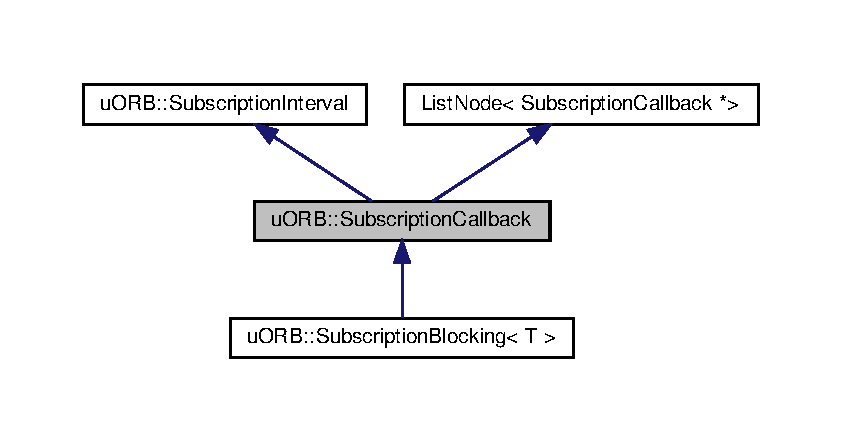
\includegraphics[width=350pt]{d6/d4a/classuORB_1_1SubscriptionCallback__inherit__graph}
\end{center}
\end{figure}


Collaboration diagram for u\+O\+RB\+:\+:Subscription\+Callback\+:\nopagebreak
\begin{figure}[H]
\begin{center}
\leavevmode
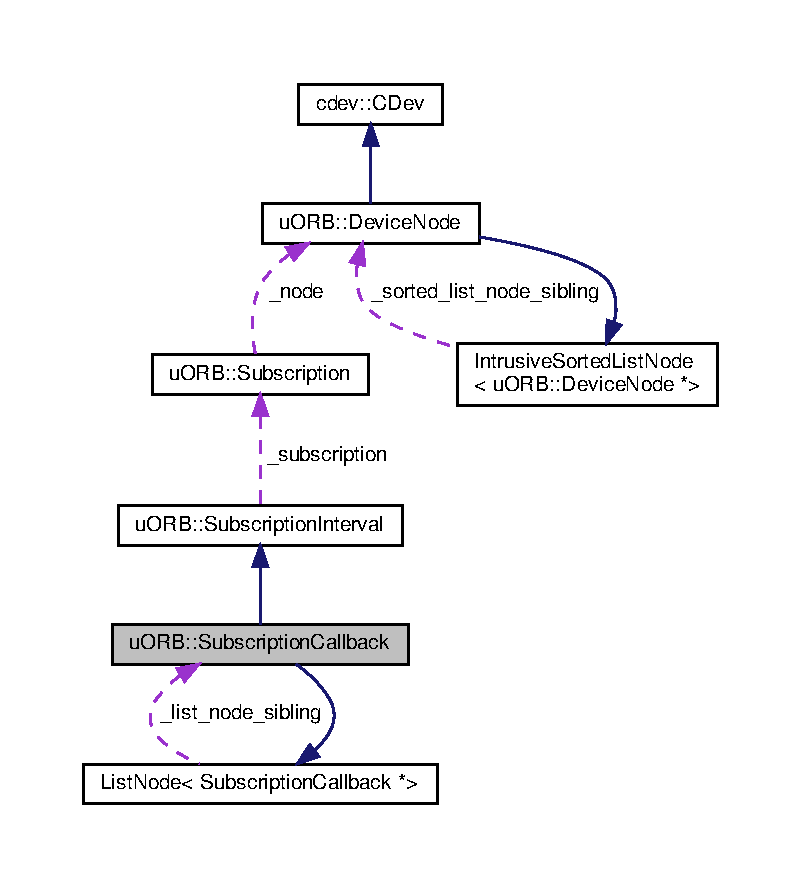
\includegraphics[width=350pt]{d1/dba/classuORB_1_1SubscriptionCallback__coll__graph}
\end{center}
\end{figure}
\subsection*{Public Member Functions}
\begin{DoxyCompactItemize}
\item 
\hyperlink{classuORB_1_1SubscriptionCallback_acc7373f302eb194d01734aedab1db772}{Subscription\+Callback} (const \hyperlink{structorb__metadata}{orb\+\_\+metadata} $\ast$meta, uint32\+\_\+t interval\+\_\+us=0, uint8\+\_\+t instance=0)
\item 
\mbox{\Hypertarget{classuORB_1_1SubscriptionCallback_a1c8b2b68441e61d7c460efe94617b3c4}\label{classuORB_1_1SubscriptionCallback_a1c8b2b68441e61d7c460efe94617b3c4}} 
bool {\bfseries register\+Callback} ()
\item 
\mbox{\Hypertarget{classuORB_1_1SubscriptionCallback_a42885c3adf9615ae6516728e295c589b}\label{classuORB_1_1SubscriptionCallback_a42885c3adf9615ae6516728e295c589b}} 
void {\bfseries unregister\+Callback} ()
\item 
bool \hyperlink{classuORB_1_1SubscriptionCallback_a63a7297780d7d29b47c25117ec3d7532}{Change\+Instance} (uint8\+\_\+t instance)
\item 
\mbox{\Hypertarget{classuORB_1_1SubscriptionCallback_a66f5f5f9f7217f855f54fbcd48e69c52}\label{classuORB_1_1SubscriptionCallback_a66f5f5f9f7217f855f54fbcd48e69c52}} 
virtual void {\bfseries call} ()=0
\end{DoxyCompactItemize}
\subsection*{Protected Attributes}
\begin{DoxyCompactItemize}
\item 
\mbox{\Hypertarget{classuORB_1_1SubscriptionCallback_ade1bb35d9dfe8bbcce3ff128f52dd964}\label{classuORB_1_1SubscriptionCallback_ade1bb35d9dfe8bbcce3ff128f52dd964}} 
bool {\bfseries \+\_\+registered} \{false\}
\end{DoxyCompactItemize}


\subsection{Detailed Description}


Definition at line 50 of file Subscription\+Callback.\+hpp.



\subsection{Constructor \& Destructor Documentation}
\mbox{\Hypertarget{classuORB_1_1SubscriptionCallback_acc7373f302eb194d01734aedab1db772}\label{classuORB_1_1SubscriptionCallback_acc7373f302eb194d01734aedab1db772}} 
\index{u\+O\+R\+B\+::\+Subscription\+Callback@{u\+O\+R\+B\+::\+Subscription\+Callback}!Subscription\+Callback@{Subscription\+Callback}}
\index{Subscription\+Callback@{Subscription\+Callback}!u\+O\+R\+B\+::\+Subscription\+Callback@{u\+O\+R\+B\+::\+Subscription\+Callback}}
\subsubsection{\texorpdfstring{Subscription\+Callback()}{SubscriptionCallback()}}
{\footnotesize\ttfamily u\+O\+R\+B\+::\+Subscription\+Callback\+::\+Subscription\+Callback (\begin{DoxyParamCaption}\item[{const \hyperlink{structorb__metadata}{orb\+\_\+metadata} $\ast$}]{meta,  }\item[{uint32\+\_\+t}]{interval\+\_\+us = {\ttfamily 0},  }\item[{uint8\+\_\+t}]{instance = {\ttfamily 0} }\end{DoxyParamCaption})\hspace{0.3cm}{\ttfamily [inline]}}

Constructor


\begin{DoxyParams}{Parameters}
{\em meta} & The u\+O\+RB metadata (usually from the \hyperlink{uORB_8h_a96af5434ec1acdf24287bd7851b0413f}{O\+R\+B\+\_\+\+I\+D()} macro) for the topic. \\
\hline
{\em interval\+\_\+us} & The requested maximum update interval in microseconds. \\
\hline
{\em instance} & The instance for multi sub. \\
\hline
\end{DoxyParams}


Definition at line 60 of file Subscription\+Callback.\+hpp.


\begin{DoxyCode}
60                                                                                                    :
61         \hyperlink{classuORB_1_1SubscriptionInterval_a7e51c851205bd12c2a973f1dbcaa91a5}{SubscriptionInterval}(meta, interval\_us, instance)
62     \{
63     \}
\end{DoxyCode}


\subsection{Member Function Documentation}
\mbox{\Hypertarget{classuORB_1_1SubscriptionCallback_a63a7297780d7d29b47c25117ec3d7532}\label{classuORB_1_1SubscriptionCallback_a63a7297780d7d29b47c25117ec3d7532}} 
\index{u\+O\+R\+B\+::\+Subscription\+Callback@{u\+O\+R\+B\+::\+Subscription\+Callback}!Change\+Instance@{Change\+Instance}}
\index{Change\+Instance@{Change\+Instance}!u\+O\+R\+B\+::\+Subscription\+Callback@{u\+O\+R\+B\+::\+Subscription\+Callback}}
\subsubsection{\texorpdfstring{Change\+Instance()}{ChangeInstance()}}
{\footnotesize\ttfamily bool u\+O\+R\+B\+::\+Subscription\+Callback\+::\+Change\+Instance (\begin{DoxyParamCaption}\item[{uint8\+\_\+t}]{instance }\end{DoxyParamCaption})\hspace{0.3cm}{\ttfamily [inline]}}

Change subscription instance 
\begin{DoxyParams}{Parameters}
{\em instance} & The new multi-\/\+Subscription instance \\
\hline
\end{DoxyParams}


Definition at line 106 of file Subscription\+Callback.\+hpp.


\begin{DoxyCode}
107     \{
108         \textcolor{keywordtype}{bool} ret = \textcolor{keyword}{false};
109 
110         \textcolor{keywordflow}{if} (instance != get\_instance()) \{
111             \textcolor{keyword}{const} \textcolor{keywordtype}{bool} registered = \_registered;
112 
113             \textcolor{keywordflow}{if} (registered) \{
114                 unregisterCallback();
115             \}
116 
117             \textcolor{keywordflow}{if} (\_subscription.\hyperlink{classuORB_1_1Subscription_a47a32a02ea909df267542d4b4ef99115}{ChangeInstance}(instance)) \{
118                 ret = \textcolor{keyword}{true};
119             \}
120 
121             \textcolor{keywordflow}{if} (registered) \{
122                 registerCallback();
123             \}
124 
125         \} \textcolor{keywordflow}{else} \{
126             \textcolor{comment}{// already on desired index}
127             \textcolor{keywordflow}{return} \textcolor{keyword}{true};
128         \}
129 
130         \textcolor{keywordflow}{return} ret;
131     \}
\end{DoxyCode}


The documentation for this class was generated from the following file\+:\begin{DoxyCompactItemize}
\item 
/home/andressanchez/\+Escritorio/\+G\+I\+T/project\+\_\+template/src/modules/u\+O\+R\+B/\hyperlink{SubscriptionCallback_8hpp}{Subscription\+Callback.\+hpp}\end{DoxyCompactItemize}

\hypertarget{classuORB_1_1SubscriptionData}{}\section{u\+O\+RB\+:\+:Subscription\+Data$<$ T $>$ Class Template Reference}
\label{classuORB_1_1SubscriptionData}\index{u\+O\+R\+B\+::\+Subscription\+Data$<$ T $>$@{u\+O\+R\+B\+::\+Subscription\+Data$<$ T $>$}}


Inheritance diagram for u\+O\+RB\+:\+:Subscription\+Data$<$ T $>$\+:\nopagebreak
\begin{figure}[H]
\begin{center}
\leavevmode
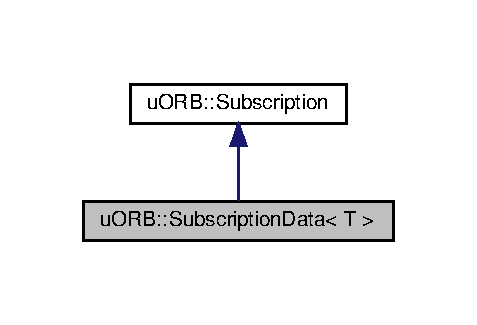
\includegraphics[width=229pt]{d0/d46/classuORB_1_1SubscriptionData__inherit__graph}
\end{center}
\end{figure}


Collaboration diagram for u\+O\+RB\+:\+:Subscription\+Data$<$ T $>$\+:\nopagebreak
\begin{figure}[H]
\begin{center}
\leavevmode
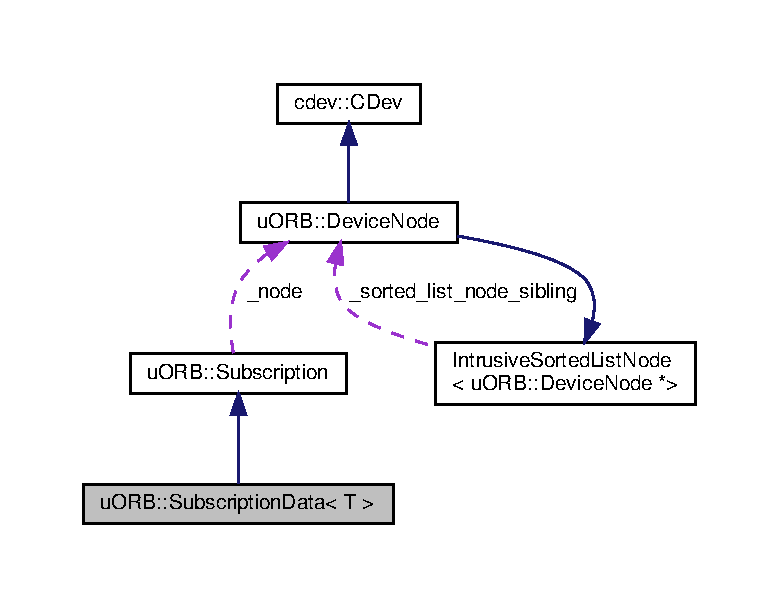
\includegraphics[width=350pt]{d6/d00/classuORB_1_1SubscriptionData__coll__graph}
\end{center}
\end{figure}
\subsection*{Public Member Functions}
\begin{DoxyCompactItemize}
\item 
\hyperlink{classuORB_1_1SubscriptionData_a7d302ca4502cbd67dee434bcbec2d819}{Subscription\+Data} (\hyperlink{uORB_8h_a96af5434ec1acdf24287bd7851b0413f}{O\+R\+B\+\_\+\+ID} id, uint8\+\_\+t instance=0)
\item 
\hyperlink{classuORB_1_1SubscriptionData_a2150e11c06c9665a8132780dc7e8e354}{Subscription\+Data} (const \hyperlink{structorb__metadata}{orb\+\_\+metadata} $\ast$meta, uint8\+\_\+t instance=0)
\item 
\mbox{\Hypertarget{classuORB_1_1SubscriptionData_a4cf78feac71104f295529342843aec20}\label{classuORB_1_1SubscriptionData_a4cf78feac71104f295529342843aec20}} 
{\bfseries Subscription\+Data} (const \hyperlink{classuORB_1_1SubscriptionData}{Subscription\+Data} \&)=delete
\item 
\mbox{\Hypertarget{classuORB_1_1SubscriptionData_a21d299cad0fed08b3a6c1cad7381887d}\label{classuORB_1_1SubscriptionData_a21d299cad0fed08b3a6c1cad7381887d}} 
\hyperlink{classuORB_1_1SubscriptionData}{Subscription\+Data} \& {\bfseries operator=} (const \hyperlink{classuORB_1_1SubscriptionData}{Subscription\+Data} \&)=delete
\item 
\mbox{\Hypertarget{classuORB_1_1SubscriptionData_a636ee6fee75fd9e3c76f56bbbc5b6f67}\label{classuORB_1_1SubscriptionData_a636ee6fee75fd9e3c76f56bbbc5b6f67}} 
{\bfseries Subscription\+Data} (\hyperlink{classuORB_1_1SubscriptionData}{Subscription\+Data} \&\&)=delete
\item 
\mbox{\Hypertarget{classuORB_1_1SubscriptionData_a378cfbe34e7ce31501789a4a7f104dc7}\label{classuORB_1_1SubscriptionData_a378cfbe34e7ce31501789a4a7f104dc7}} 
\hyperlink{classuORB_1_1SubscriptionData}{Subscription\+Data} \& {\bfseries operator=} (\hyperlink{classuORB_1_1SubscriptionData}{Subscription\+Data} \&\&)=delete
\item 
\mbox{\Hypertarget{classuORB_1_1SubscriptionData_a8c8967077b39cd29e07652cefe2293a9}\label{classuORB_1_1SubscriptionData_a8c8967077b39cd29e07652cefe2293a9}} 
bool {\bfseries update} ()
\item 
\mbox{\Hypertarget{classuORB_1_1SubscriptionData_ab75614b7adbc3ba5cbf0c3ec82e70fd2}\label{classuORB_1_1SubscriptionData_ab75614b7adbc3ba5cbf0c3ec82e70fd2}} 
const T \& {\bfseries get} () const
\end{DoxyCompactItemize}
\subsection*{Additional Inherited Members}


\subsection{Detailed Description}
\subsubsection*{template$<$class T$>$\newline
class u\+O\+R\+B\+::\+Subscription\+Data$<$ T $>$}



Definition at line 158 of file Subscription.\+hpp.



\subsection{Constructor \& Destructor Documentation}
\mbox{\Hypertarget{classuORB_1_1SubscriptionData_a7d302ca4502cbd67dee434bcbec2d819}\label{classuORB_1_1SubscriptionData_a7d302ca4502cbd67dee434bcbec2d819}} 
\index{u\+O\+R\+B\+::\+Subscription\+Data@{u\+O\+R\+B\+::\+Subscription\+Data}!Subscription\+Data@{Subscription\+Data}}
\index{Subscription\+Data@{Subscription\+Data}!u\+O\+R\+B\+::\+Subscription\+Data@{u\+O\+R\+B\+::\+Subscription\+Data}}
\subsubsection{\texorpdfstring{Subscription\+Data()}{SubscriptionData()}\hspace{0.1cm}{\footnotesize\ttfamily [1/2]}}
{\footnotesize\ttfamily template$<$class T $>$ \\
\hyperlink{classuORB_1_1SubscriptionData}{u\+O\+R\+B\+::\+Subscription\+Data}$<$ T $>$\+::\hyperlink{classuORB_1_1SubscriptionData}{Subscription\+Data} (\begin{DoxyParamCaption}\item[{\hyperlink{uORB_8h_a96af5434ec1acdf24287bd7851b0413f}{O\+R\+B\+\_\+\+ID}}]{id,  }\item[{uint8\+\_\+t}]{instance = {\ttfamily 0} }\end{DoxyParamCaption})\hspace{0.3cm}{\ttfamily [inline]}}

Constructor


\begin{DoxyParams}{Parameters}
{\em id} & The u\+O\+RB metadata O\+R\+B\+\_\+\+ID enum for the topic. \\
\hline
{\em instance} & The instance for multi sub. \\
\hline
\end{DoxyParams}


Definition at line 167 of file Subscription.\+hpp.


\begin{DoxyCode}
167                                                       :
168         \hyperlink{classuORB_1_1Subscription_a6afd37f8aa13bc3ffeafd29b7a3d434f}{Subscription}(\textcolor{keywordtype}{id}, instance)
169     \{
170         \hyperlink{classuORB_1_1Subscription_a17a37eb5624b409379db434400de4582}{copy}(&\_data);
171     \}
\end{DoxyCode}
\mbox{\Hypertarget{classuORB_1_1SubscriptionData_a2150e11c06c9665a8132780dc7e8e354}\label{classuORB_1_1SubscriptionData_a2150e11c06c9665a8132780dc7e8e354}} 
\index{u\+O\+R\+B\+::\+Subscription\+Data@{u\+O\+R\+B\+::\+Subscription\+Data}!Subscription\+Data@{Subscription\+Data}}
\index{Subscription\+Data@{Subscription\+Data}!u\+O\+R\+B\+::\+Subscription\+Data@{u\+O\+R\+B\+::\+Subscription\+Data}}
\subsubsection{\texorpdfstring{Subscription\+Data()}{SubscriptionData()}\hspace{0.1cm}{\footnotesize\ttfamily [2/2]}}
{\footnotesize\ttfamily template$<$class T $>$ \\
\hyperlink{classuORB_1_1SubscriptionData}{u\+O\+R\+B\+::\+Subscription\+Data}$<$ T $>$\+::\hyperlink{classuORB_1_1SubscriptionData}{Subscription\+Data} (\begin{DoxyParamCaption}\item[{const \hyperlink{structorb__metadata}{orb\+\_\+metadata} $\ast$}]{meta,  }\item[{uint8\+\_\+t}]{instance = {\ttfamily 0} }\end{DoxyParamCaption})\hspace{0.3cm}{\ttfamily [inline]}}

Constructor


\begin{DoxyParams}{Parameters}
{\em meta} & The u\+O\+RB metadata (usually from the \hyperlink{uORB_8h_a96af5434ec1acdf24287bd7851b0413f}{O\+R\+B\+\_\+\+I\+D()} macro) for the topic. \\
\hline
{\em instance} & The instance for multi sub. \\
\hline
\end{DoxyParams}


Definition at line 179 of file Subscription.\+hpp.


\begin{DoxyCode}
179                                                                      :
180         \hyperlink{classuORB_1_1Subscription_a6afd37f8aa13bc3ffeafd29b7a3d434f}{Subscription}(meta, instance)
181     \{
182         \hyperlink{classuORB_1_1Subscription_a17a37eb5624b409379db434400de4582}{copy}(&\_data);
183     \}
\end{DoxyCode}


The documentation for this class was generated from the following file\+:\begin{DoxyCompactItemize}
\item 
/home/andressanchez/\+Escritorio/\+G\+I\+T/project\+\_\+template/src/modules/u\+O\+R\+B/\hyperlink{Subscription_8hpp}{Subscription.\+hpp}\end{DoxyCompactItemize}

\hypertarget{classuORB_1_1SubscriptionInterval}{}\section{u\+O\+RB\+:\+:Subscription\+Interval Class Reference}
\label{classuORB_1_1SubscriptionInterval}\index{u\+O\+R\+B\+::\+Subscription\+Interval@{u\+O\+R\+B\+::\+Subscription\+Interval}}


Inheritance diagram for u\+O\+RB\+:\+:Subscription\+Interval\+:\nopagebreak
\begin{figure}[H]
\begin{center}
\leavevmode
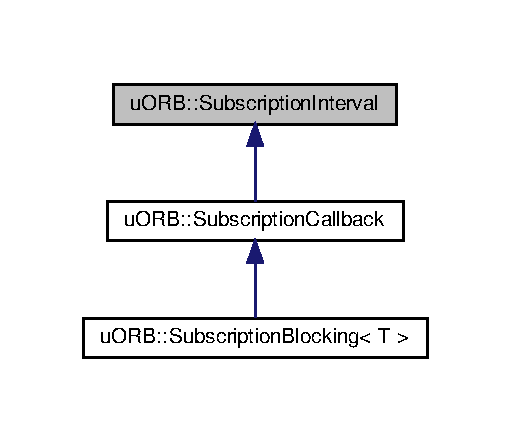
\includegraphics[width=245pt]{dd/ded/classuORB_1_1SubscriptionInterval__inherit__graph}
\end{center}
\end{figure}


Collaboration diagram for u\+O\+RB\+:\+:Subscription\+Interval\+:\nopagebreak
\begin{figure}[H]
\begin{center}
\leavevmode
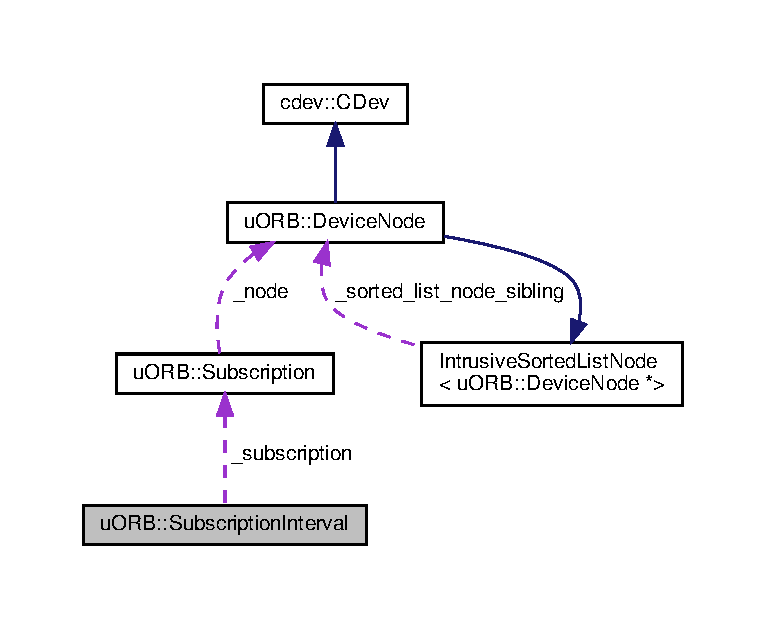
\includegraphics[width=350pt]{d2/d4f/classuORB_1_1SubscriptionInterval__coll__graph}
\end{center}
\end{figure}
\subsection*{Public Member Functions}
\begin{DoxyCompactItemize}
\item 
\hyperlink{classuORB_1_1SubscriptionInterval_a7e51c851205bd12c2a973f1dbcaa91a5}{Subscription\+Interval} (\hyperlink{uORB_8h_a96af5434ec1acdf24287bd7851b0413f}{O\+R\+B\+\_\+\+ID} id, uint32\+\_\+t interval\+\_\+us=0, uint8\+\_\+t instance=0)
\item 
\hyperlink{classuORB_1_1SubscriptionInterval_a5484a71c5ad98ca70bfa88d8de9550af}{Subscription\+Interval} (const \hyperlink{structorb__metadata}{orb\+\_\+metadata} $\ast$meta, uint32\+\_\+t interval\+\_\+us=0, uint8\+\_\+t instance=0)
\item 
\mbox{\Hypertarget{classuORB_1_1SubscriptionInterval_a1febf0b92009d71a8866e759c6fc0e6d}\label{classuORB_1_1SubscriptionInterval_a1febf0b92009d71a8866e759c6fc0e6d}} 
bool {\bfseries subscribe} ()
\item 
\mbox{\Hypertarget{classuORB_1_1SubscriptionInterval_aa1b4d9eac19750eedc7c809c88a0534c}\label{classuORB_1_1SubscriptionInterval_aa1b4d9eac19750eedc7c809c88a0534c}} 
void {\bfseries unsubscribe} ()
\item 
\mbox{\Hypertarget{classuORB_1_1SubscriptionInterval_ad37eaf4990b69463eb3f3c53db76874d}\label{classuORB_1_1SubscriptionInterval_ad37eaf4990b69463eb3f3c53db76874d}} 
bool {\bfseries advertised} ()
\item 
bool \hyperlink{classuORB_1_1SubscriptionInterval_aa1c12b83d65604e306b919a2c224e32e}{updated} ()
\item 
bool \hyperlink{classuORB_1_1SubscriptionInterval_ac9198cc23c666df10af2a8fb3f809508}{update} (void $\ast$dst)
\item 
bool \hyperlink{classuORB_1_1SubscriptionInterval_a25125ed09772665d3b4b4e6978fb3e1c}{copy} (void $\ast$dst)
\item 
\mbox{\Hypertarget{classuORB_1_1SubscriptionInterval_a82ac3efc49cc896017552f277a6ae003}\label{classuORB_1_1SubscriptionInterval_a82ac3efc49cc896017552f277a6ae003}} 
bool {\bfseries valid} () const
\item 
\mbox{\Hypertarget{classuORB_1_1SubscriptionInterval_a93e8f0a9b49c1f38b3a68f725fef4ab5}\label{classuORB_1_1SubscriptionInterval_a93e8f0a9b49c1f38b3a68f725fef4ab5}} 
uint8\+\_\+t {\bfseries get\+\_\+instance} () const
\item 
\mbox{\Hypertarget{classuORB_1_1SubscriptionInterval_a3ef43a25c5bb473b5e8e86a57a1b0387}\label{classuORB_1_1SubscriptionInterval_a3ef43a25c5bb473b5e8e86a57a1b0387}} 
uint32\+\_\+t {\bfseries get\+\_\+interval\+\_\+us} () const
\item 
\mbox{\Hypertarget{classuORB_1_1SubscriptionInterval_a70f0db8ef87cbe335c01b7a24bb0eaf2}\label{classuORB_1_1SubscriptionInterval_a70f0db8ef87cbe335c01b7a24bb0eaf2}} 
unsigned {\bfseries get\+\_\+last\+\_\+generation} () const
\item 
\mbox{\Hypertarget{classuORB_1_1SubscriptionInterval_a2e625fde36b8501430a7c0518521286f}\label{classuORB_1_1SubscriptionInterval_a2e625fde36b8501430a7c0518521286f}} 
\hyperlink{structorb__metadata}{orb\+\_\+id\+\_\+t} {\bfseries get\+\_\+topic} () const
\item 
void \hyperlink{classuORB_1_1SubscriptionInterval_a53018b44bb431a80d47ac95327990b2a}{set\+\_\+interval\+\_\+us} (uint32\+\_\+t interval)
\item 
void \hyperlink{classuORB_1_1SubscriptionInterval_a12e68cbb4d69d82ec586aa2bbc8e9672}{set\+\_\+interval\+\_\+ms} (uint32\+\_\+t interval)
\end{DoxyCompactItemize}
\subsection*{Protected Attributes}
\begin{DoxyCompactItemize}
\item 
\mbox{\Hypertarget{classuORB_1_1SubscriptionInterval_a9e90aab2e7af7acfc36282d438fa2741}\label{classuORB_1_1SubscriptionInterval_a9e90aab2e7af7acfc36282d438fa2741}} 
\hyperlink{classuORB_1_1Subscription}{Subscription} {\bfseries \+\_\+subscription}
\item 
\mbox{\Hypertarget{classuORB_1_1SubscriptionInterval_ac1cdffa27e2a8393a2111a996b4f05bf}\label{classuORB_1_1SubscriptionInterval_ac1cdffa27e2a8393a2111a996b4f05bf}} 
uint64\+\_\+t {\bfseries \+\_\+last\+\_\+update} \{0\}
\item 
\mbox{\Hypertarget{classuORB_1_1SubscriptionInterval_a01c7991b993e3851bc110b84dc485ed9}\label{classuORB_1_1SubscriptionInterval_a01c7991b993e3851bc110b84dc485ed9}} 
uint32\+\_\+t {\bfseries \+\_\+interval\+\_\+us} \{0\}
\end{DoxyCompactItemize}


\subsection{Detailed Description}


Definition at line 55 of file Subscription\+Interval.\+hpp.



\subsection{Constructor \& Destructor Documentation}
\mbox{\Hypertarget{classuORB_1_1SubscriptionInterval_a7e51c851205bd12c2a973f1dbcaa91a5}\label{classuORB_1_1SubscriptionInterval_a7e51c851205bd12c2a973f1dbcaa91a5}} 
\index{u\+O\+R\+B\+::\+Subscription\+Interval@{u\+O\+R\+B\+::\+Subscription\+Interval}!Subscription\+Interval@{Subscription\+Interval}}
\index{Subscription\+Interval@{Subscription\+Interval}!u\+O\+R\+B\+::\+Subscription\+Interval@{u\+O\+R\+B\+::\+Subscription\+Interval}}
\subsubsection{\texorpdfstring{Subscription\+Interval()}{SubscriptionInterval()}\hspace{0.1cm}{\footnotesize\ttfamily [1/2]}}
{\footnotesize\ttfamily u\+O\+R\+B\+::\+Subscription\+Interval\+::\+Subscription\+Interval (\begin{DoxyParamCaption}\item[{\hyperlink{uORB_8h_a96af5434ec1acdf24287bd7851b0413f}{O\+R\+B\+\_\+\+ID}}]{id,  }\item[{uint32\+\_\+t}]{interval\+\_\+us = {\ttfamily 0},  }\item[{uint8\+\_\+t}]{instance = {\ttfamily 0} }\end{DoxyParamCaption})\hspace{0.3cm}{\ttfamily [inline]}}

Constructor


\begin{DoxyParams}{Parameters}
{\em id} & The u\+O\+RB O\+R\+B\+\_\+\+ID enum for the topic. \\
\hline
{\em interval} & The requested maximum update interval in microseconds. \\
\hline
{\em instance} & The instance for multi sub. \\
\hline
\end{DoxyParams}


Definition at line 66 of file Subscription\+Interval.\+hpp.


\begin{DoxyCode}
66                                                                                     :
67         \_subscription\{id, instance\},
68         \_interval\_us(interval\_us)
69     \{\}
\end{DoxyCode}
\mbox{\Hypertarget{classuORB_1_1SubscriptionInterval_a5484a71c5ad98ca70bfa88d8de9550af}\label{classuORB_1_1SubscriptionInterval_a5484a71c5ad98ca70bfa88d8de9550af}} 
\index{u\+O\+R\+B\+::\+Subscription\+Interval@{u\+O\+R\+B\+::\+Subscription\+Interval}!Subscription\+Interval@{Subscription\+Interval}}
\index{Subscription\+Interval@{Subscription\+Interval}!u\+O\+R\+B\+::\+Subscription\+Interval@{u\+O\+R\+B\+::\+Subscription\+Interval}}
\subsubsection{\texorpdfstring{Subscription\+Interval()}{SubscriptionInterval()}\hspace{0.1cm}{\footnotesize\ttfamily [2/2]}}
{\footnotesize\ttfamily u\+O\+R\+B\+::\+Subscription\+Interval\+::\+Subscription\+Interval (\begin{DoxyParamCaption}\item[{const \hyperlink{structorb__metadata}{orb\+\_\+metadata} $\ast$}]{meta,  }\item[{uint32\+\_\+t}]{interval\+\_\+us = {\ttfamily 0},  }\item[{uint8\+\_\+t}]{instance = {\ttfamily 0} }\end{DoxyParamCaption})\hspace{0.3cm}{\ttfamily [inline]}}

Constructor


\begin{DoxyParams}{Parameters}
{\em meta} & The u\+O\+RB metadata (usually from the \hyperlink{uORB_8h_a96af5434ec1acdf24287bd7851b0413f}{O\+R\+B\+\_\+\+I\+D()} macro) for the topic. \\
\hline
{\em interval} & The requested maximum update interval in microseconds. \\
\hline
{\em instance} & The instance for multi sub. \\
\hline
\end{DoxyParams}


Definition at line 78 of file Subscription\+Interval.\+hpp.


\begin{DoxyCode}
78                                                                                                    :
79         \_subscription\{meta, instance\},
80         \_interval\_us(interval\_us)
81     \{\}
\end{DoxyCode}


\subsection{Member Function Documentation}
\mbox{\Hypertarget{classuORB_1_1SubscriptionInterval_a25125ed09772665d3b4b4e6978fb3e1c}\label{classuORB_1_1SubscriptionInterval_a25125ed09772665d3b4b4e6978fb3e1c}} 
\index{u\+O\+R\+B\+::\+Subscription\+Interval@{u\+O\+R\+B\+::\+Subscription\+Interval}!copy@{copy}}
\index{copy@{copy}!u\+O\+R\+B\+::\+Subscription\+Interval@{u\+O\+R\+B\+::\+Subscription\+Interval}}
\subsubsection{\texorpdfstring{copy()}{copy()}}
{\footnotesize\ttfamily bool u\+O\+R\+B\+::\+Subscription\+Interval\+::copy (\begin{DoxyParamCaption}\item[{void $\ast$}]{dst }\end{DoxyParamCaption})\hspace{0.3cm}{\ttfamily [inline]}}

Copy the struct 
\begin{DoxyParams}{Parameters}
{\em dst} & The destination pointer where the struct will be copied. \\
\hline
\end{DoxyParams}
\begin{DoxyReturn}{Returns}
true only if topic was copied successfully. 
\end{DoxyReturn}


Definition at line 123 of file Subscription\+Interval.\+hpp.


\begin{DoxyCode}
124     \{
125         \textcolor{keywordflow}{if} (\_subscription.\hyperlink{classuORB_1_1Subscription_a17a37eb5624b409379db434400de4582}{copy}(dst)) \{
126             \textcolor{comment}{//const hrtime\_t now = gethrtime();}
127             \textcolor{keyword}{const} \hyperlink{drv__hrt_8h_a9f8bbf0e883115e04a457a268533a87c}{hrt\_abstime} now = \hyperlink{drv__hrt_8h_a91f4291796ed7fbe544dc22ee5288367}{hrt\_absolute\_time}();
128             \textcolor{comment}{// shift last update time forward, but don't let it get further behind than the interval}
129             \_last\_update = math::constrain(\_last\_update + \_interval\_us, now - \_interval\_us, now);
130             \textcolor{keywordflow}{return} \textcolor{keyword}{true};
131         \}
132 
133         \textcolor{keywordflow}{return} \textcolor{keyword}{false};
134     \}
\end{DoxyCode}
\mbox{\Hypertarget{classuORB_1_1SubscriptionInterval_a12e68cbb4d69d82ec586aa2bbc8e9672}\label{classuORB_1_1SubscriptionInterval_a12e68cbb4d69d82ec586aa2bbc8e9672}} 
\index{u\+O\+R\+B\+::\+Subscription\+Interval@{u\+O\+R\+B\+::\+Subscription\+Interval}!set\+\_\+interval\+\_\+ms@{set\+\_\+interval\+\_\+ms}}
\index{set\+\_\+interval\+\_\+ms@{set\+\_\+interval\+\_\+ms}!u\+O\+R\+B\+::\+Subscription\+Interval@{u\+O\+R\+B\+::\+Subscription\+Interval}}
\subsubsection{\texorpdfstring{set\+\_\+interval\+\_\+ms()}{set\_interval\_ms()}}
{\footnotesize\ttfamily void u\+O\+R\+B\+::\+Subscription\+Interval\+::set\+\_\+interval\+\_\+ms (\begin{DoxyParamCaption}\item[{uint32\+\_\+t}]{interval }\end{DoxyParamCaption})\hspace{0.3cm}{\ttfamily [inline]}}

Set the interval in milliseconds 
\begin{DoxyParams}{Parameters}
{\em interval} & The interval in milliseconds. \\
\hline
\end{DoxyParams}


Definition at line 153 of file Subscription\+Interval.\+hpp.


\begin{DoxyCode}
153 \{ \_interval\_us = interval * 1000; \}
\end{DoxyCode}
\mbox{\Hypertarget{classuORB_1_1SubscriptionInterval_a53018b44bb431a80d47ac95327990b2a}\label{classuORB_1_1SubscriptionInterval_a53018b44bb431a80d47ac95327990b2a}} 
\index{u\+O\+R\+B\+::\+Subscription\+Interval@{u\+O\+R\+B\+::\+Subscription\+Interval}!set\+\_\+interval\+\_\+us@{set\+\_\+interval\+\_\+us}}
\index{set\+\_\+interval\+\_\+us@{set\+\_\+interval\+\_\+us}!u\+O\+R\+B\+::\+Subscription\+Interval@{u\+O\+R\+B\+::\+Subscription\+Interval}}
\subsubsection{\texorpdfstring{set\+\_\+interval\+\_\+us()}{set\_interval\_us()}}
{\footnotesize\ttfamily void u\+O\+R\+B\+::\+Subscription\+Interval\+::set\+\_\+interval\+\_\+us (\begin{DoxyParamCaption}\item[{uint32\+\_\+t}]{interval }\end{DoxyParamCaption})\hspace{0.3cm}{\ttfamily [inline]}}

Set the interval in microseconds 
\begin{DoxyParams}{Parameters}
{\em interval} & The interval in microseconds. \\
\hline
\end{DoxyParams}


Definition at line 147 of file Subscription\+Interval.\+hpp.


\begin{DoxyCode}
147 \{ \_interval\_us = interval; \}
\end{DoxyCode}
\mbox{\Hypertarget{classuORB_1_1SubscriptionInterval_ac9198cc23c666df10af2a8fb3f809508}\label{classuORB_1_1SubscriptionInterval_ac9198cc23c666df10af2a8fb3f809508}} 
\index{u\+O\+R\+B\+::\+Subscription\+Interval@{u\+O\+R\+B\+::\+Subscription\+Interval}!update@{update}}
\index{update@{update}!u\+O\+R\+B\+::\+Subscription\+Interval@{u\+O\+R\+B\+::\+Subscription\+Interval}}
\subsubsection{\texorpdfstring{update()}{update()}}
{\footnotesize\ttfamily bool u\+O\+R\+B\+::\+Subscription\+Interval\+::update (\begin{DoxyParamCaption}\item[{void $\ast$}]{dst }\end{DoxyParamCaption})\hspace{0.3cm}{\ttfamily [inline]}}

Copy the struct if updated. 
\begin{DoxyParams}{Parameters}
{\em dst} & The destination pointer where the struct will be copied. \\
\hline
\end{DoxyParams}
\begin{DoxyReturn}{Returns}
true only if topic was updated and copied successfully. 
\end{DoxyReturn}


Definition at line 109 of file Subscription\+Interval.\+hpp.


\begin{DoxyCode}
110     \{
111         \textcolor{keywordflow}{if} (\hyperlink{classuORB_1_1SubscriptionInterval_aa1c12b83d65604e306b919a2c224e32e}{updated}()) \{
112             \textcolor{keywordflow}{return} \hyperlink{classuORB_1_1SubscriptionInterval_a25125ed09772665d3b4b4e6978fb3e1c}{copy}(dst);
113         \}
114 
115         \textcolor{keywordflow}{return} \textcolor{keyword}{false};
116     \}
\end{DoxyCode}
\mbox{\Hypertarget{classuORB_1_1SubscriptionInterval_aa1c12b83d65604e306b919a2c224e32e}\label{classuORB_1_1SubscriptionInterval_aa1c12b83d65604e306b919a2c224e32e}} 
\index{u\+O\+R\+B\+::\+Subscription\+Interval@{u\+O\+R\+B\+::\+Subscription\+Interval}!updated@{updated}}
\index{updated@{updated}!u\+O\+R\+B\+::\+Subscription\+Interval@{u\+O\+R\+B\+::\+Subscription\+Interval}}
\subsubsection{\texorpdfstring{updated()}{updated()}}
{\footnotesize\ttfamily bool u\+O\+R\+B\+::\+Subscription\+Interval\+::updated (\begin{DoxyParamCaption}{ }\end{DoxyParamCaption})\hspace{0.3cm}{\ttfamily [inline]}}

Check if there is a new update. 

Definition at line 95 of file Subscription\+Interval.\+hpp.


\begin{DoxyCode}
96     \{
97         \textcolor{keywordflow}{if} (advertised() && (hrt\_elapsed\_time(&\_last\_update) >= \_interval\_us)) \{
98             \textcolor{keywordflow}{return} \_subscription.\hyperlink{classuORB_1_1Subscription_a788d1848a46abe88a093be9a1f7cb2ca}{updated}();
99         \}
100 
101         \textcolor{keywordflow}{return} \textcolor{keyword}{false};
102     \}
\end{DoxyCode}


The documentation for this class was generated from the following file\+:\begin{DoxyCompactItemize}
\item 
/home/andressanchez/\+Escritorio/\+G\+I\+T/project\+\_\+template/src/modules/u\+O\+R\+B/\hyperlink{SubscriptionInterval_8hpp}{Subscription\+Interval.\+hpp}\end{DoxyCompactItemize}

\hypertarget{classuORB_1_1SubscriptionMultiArray}{}\section{u\+O\+RB\+:\+:Subscription\+Multi\+Array$<$ T, S\+I\+ZE $>$ Class Template Reference}
\label{classuORB_1_1SubscriptionMultiArray}\index{u\+O\+R\+B\+::\+Subscription\+Multi\+Array$<$ T, S\+I\+Z\+E $>$@{u\+O\+R\+B\+::\+Subscription\+Multi\+Array$<$ T, S\+I\+Z\+E $>$}}


{\ttfamily \#include $<$Subscription\+Multi\+Array.\+hpp$>$}

\subsection*{Public Member Functions}
\begin{DoxyCompactItemize}
\item 
\hyperlink{classuORB_1_1SubscriptionMultiArray_a36aea582175575ace4386505434670af}{Subscription\+Multi\+Array} (\hyperlink{uORB_8h_a96af5434ec1acdf24287bd7851b0413f}{O\+R\+B\+\_\+\+ID} id)
\item 
\mbox{\Hypertarget{classuORB_1_1SubscriptionMultiArray_a964f7886e2be21d493f6d107cb85704c}\label{classuORB_1_1SubscriptionMultiArray_a964f7886e2be21d493f6d107cb85704c}} 
\hyperlink{classuORB_1_1SubscriptionInterval}{Subscription\+Interval} \& {\bfseries operator\mbox{[}$\,$\mbox{]}} (int i)
\item 
\mbox{\Hypertarget{classuORB_1_1SubscriptionMultiArray_a97ad1750e9cff53806105e1f73ec91fd}\label{classuORB_1_1SubscriptionMultiArray_a97ad1750e9cff53806105e1f73ec91fd}} 
const \hyperlink{classuORB_1_1SubscriptionInterval}{Subscription\+Interval} \& {\bfseries operator\mbox{[}$\,$\mbox{]}} (int i) const
\item 
\mbox{\Hypertarget{classuORB_1_1SubscriptionMultiArray_aea5115f1dc015ee12bfcdbee8cdcfa14}\label{classuORB_1_1SubscriptionMultiArray_aea5115f1dc015ee12bfcdbee8cdcfa14}} 
\hyperlink{classuORB_1_1SubscriptionInterval}{Subscription\+Interval} $\ast$ {\bfseries begin} ()
\item 
\mbox{\Hypertarget{classuORB_1_1SubscriptionMultiArray_ad17e83d98526f4d2376688e20fadb0bb}\label{classuORB_1_1SubscriptionMultiArray_ad17e83d98526f4d2376688e20fadb0bb}} 
\hyperlink{classuORB_1_1SubscriptionInterval}{Subscription\+Interval} $\ast$ {\bfseries end} ()
\item 
\mbox{\Hypertarget{classuORB_1_1SubscriptionMultiArray_a519d1832a1dcd343716a765021359021}\label{classuORB_1_1SubscriptionMultiArray_a519d1832a1dcd343716a765021359021}} 
const \hyperlink{classuORB_1_1SubscriptionInterval}{Subscription\+Interval} $\ast$ {\bfseries begin} () const
\item 
\mbox{\Hypertarget{classuORB_1_1SubscriptionMultiArray_a49779c8e56a88f1d375c371060b2c9ba}\label{classuORB_1_1SubscriptionMultiArray_a49779c8e56a88f1d375c371060b2c9ba}} 
const \hyperlink{classuORB_1_1SubscriptionInterval}{Subscription\+Interval} $\ast$ {\bfseries end} () const
\item 
\mbox{\Hypertarget{classuORB_1_1SubscriptionMultiArray_ae0f40d8b769e5e767a0c9ca005beb7ee}\label{classuORB_1_1SubscriptionMultiArray_ae0f40d8b769e5e767a0c9ca005beb7ee}} 
bool {\bfseries advertised} ()
\item 
\mbox{\Hypertarget{classuORB_1_1SubscriptionMultiArray_a189ced9653facfa05f9b561eb9a44c13}\label{classuORB_1_1SubscriptionMultiArray_a189ced9653facfa05f9b561eb9a44c13}} 
uint8\+\_\+t {\bfseries advertised\+\_\+count} ()
\item 
\mbox{\Hypertarget{classuORB_1_1SubscriptionMultiArray_afe1a493e50fd0004678064fefff336a4}\label{classuORB_1_1SubscriptionMultiArray_afe1a493e50fd0004678064fefff336a4}} 
bool {\bfseries updated} ()
\end{DoxyCompactItemize}
\subsection*{Static Public Member Functions}
\begin{DoxyCompactItemize}
\item 
\mbox{\Hypertarget{classuORB_1_1SubscriptionMultiArray_a4d8b0085665e29c0259192f5d4063fcd}\label{classuORB_1_1SubscriptionMultiArray_a4d8b0085665e29c0259192f5d4063fcd}} 
static constexpr uint8\+\_\+t {\bfseries size} ()
\end{DoxyCompactItemize}


\subsection{Detailed Description}
\subsubsection*{template$<$typename T, uint8\+\_\+t S\+I\+ZE = O\+R\+B\+\_\+\+M\+U\+L\+T\+I\+\_\+\+M\+A\+X\+\_\+\+I\+N\+S\+T\+A\+N\+C\+ES$>$\newline
class u\+O\+R\+B\+::\+Subscription\+Multi\+Array$<$ T, S\+I\+Z\+E $>$}

An array of u\+O\+R\+B\+::\+Subscriptions of the same topic 

Definition at line 55 of file Subscription\+Multi\+Array.\+hpp.



\subsection{Constructor \& Destructor Documentation}
\mbox{\Hypertarget{classuORB_1_1SubscriptionMultiArray_a36aea582175575ace4386505434670af}\label{classuORB_1_1SubscriptionMultiArray_a36aea582175575ace4386505434670af}} 
\index{u\+O\+R\+B\+::\+Subscription\+Multi\+Array@{u\+O\+R\+B\+::\+Subscription\+Multi\+Array}!Subscription\+Multi\+Array@{Subscription\+Multi\+Array}}
\index{Subscription\+Multi\+Array@{Subscription\+Multi\+Array}!u\+O\+R\+B\+::\+Subscription\+Multi\+Array@{u\+O\+R\+B\+::\+Subscription\+Multi\+Array}}
\subsubsection{\texorpdfstring{Subscription\+Multi\+Array()}{SubscriptionMultiArray()}}
{\footnotesize\ttfamily template$<$typename T , uint8\+\_\+t S\+I\+ZE = O\+R\+B\+\_\+\+M\+U\+L\+T\+I\+\_\+\+M\+A\+X\+\_\+\+I\+N\+S\+T\+A\+N\+C\+ES$>$ \\
\hyperlink{classuORB_1_1SubscriptionMultiArray}{u\+O\+R\+B\+::\+Subscription\+Multi\+Array}$<$ T, S\+I\+ZE $>$\+::\hyperlink{classuORB_1_1SubscriptionMultiArray}{Subscription\+Multi\+Array} (\begin{DoxyParamCaption}\item[{\hyperlink{uORB_8h_a96af5434ec1acdf24287bd7851b0413f}{O\+R\+B\+\_\+\+ID}}]{id }\end{DoxyParamCaption})\hspace{0.3cm}{\ttfamily [inline]}, {\ttfamily [explicit]}}

Constructor


\begin{DoxyParams}{Parameters}
{\em id} & The u\+O\+RB O\+R\+B\+\_\+\+ID enum for the topic. \\
\hline
\end{DoxyParams}


Definition at line 67 of file Subscription\+Multi\+Array.\+hpp.


\begin{DoxyCode}
68     \{
69         \textcolor{keywordflow}{for} (uint8\_t i = 0; i < SIZE; i++) \{
70             \_subscriptions[i] = SubscriptionInterval\{id, 0, i\};
71             \_subscriptions[i].subscribe();
72         \}
73     \}
\end{DoxyCode}


The documentation for this class was generated from the following file\+:\begin{DoxyCompactItemize}
\item 
/home/andressanchez/\+Escritorio/\+G\+I\+T/project\+\_\+template/src/modules/u\+O\+R\+B/\hyperlink{SubscriptionMultiArray_8hpp}{Subscription\+Multi\+Array.\+hpp}\end{DoxyCompactItemize}

\hypertarget{classTemplateModule}{}\section{Template\+Module Class Reference}
\label{classTemplateModule}\index{Template\+Module@{Template\+Module}}


Inheritance diagram for Template\+Module\+:\nopagebreak
\begin{figure}[H]
\begin{center}
\leavevmode
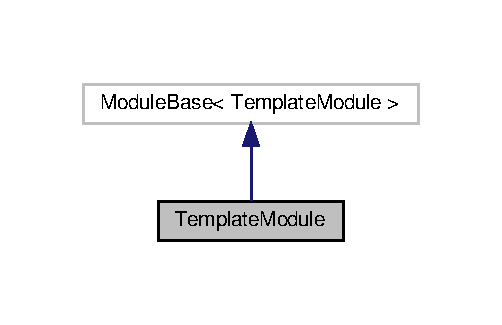
\includegraphics[width=241pt]{d0/df9/classTemplateModule__inherit__graph}
\end{center}
\end{figure}


Collaboration diagram for Template\+Module\+:\nopagebreak
\begin{figure}[H]
\begin{center}
\leavevmode
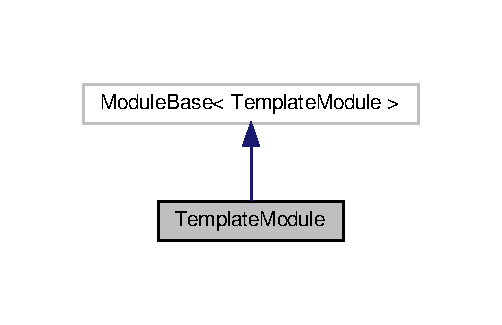
\includegraphics[width=241pt]{db/d74/classTemplateModule__coll__graph}
\end{center}
\end{figure}
\subsection*{Public Member Functions}
\begin{DoxyCompactItemize}
\item 
\mbox{\Hypertarget{classTemplateModule_a380d8124f74b33afe7388cd2e0d4a38e}\label{classTemplateModule_a380d8124f74b33afe7388cd2e0d4a38e}} 
{\bfseries Template\+Module} (int example\+\_\+param, bool example\+\_\+flag)
\item 
void \hyperlink{classTemplateModule_a9ee1970fb39e76ae38e838df00e7a058}{run} () override
\item 
int \hyperlink{classTemplateModule_a0a5e50f74b8a4bc4d3102eb1487efc88}{print\+\_\+status} () override
\end{DoxyCompactItemize}
\subsection*{Static Public Member Functions}
\begin{DoxyCompactItemize}
\item 
static int \hyperlink{classTemplateModule_a442b58c36fd9a84d34c6c2ca5da30500}{task\+\_\+spawn} (int argc, char $\ast$argv\mbox{[}$\,$\mbox{]})
\item 
static \hyperlink{classTemplateModule}{Template\+Module} $\ast$ \hyperlink{classTemplateModule_aa31cbf48b351f5ee0b33b3cbd5b8e536}{instantiate} (int argc, char $\ast$argv\mbox{[}$\,$\mbox{]})
\item 
static int \hyperlink{classTemplateModule_aa8b46132f5dcab9299e34ff43e2d6db5}{custom\+\_\+command} (int argc, char $\ast$argv\mbox{[}$\,$\mbox{]})
\item 
static int \hyperlink{classTemplateModule_a5ce5da37ebb624d8fbf301343d0ed341}{print\+\_\+usage} (const char $\ast$reason=nullptr)
\end{DoxyCompactItemize}


\subsection{Detailed Description}


Definition at line 46 of file template\+\_\+module.\+h.



\subsection{Member Function Documentation}
\mbox{\Hypertarget{classTemplateModule_aa8b46132f5dcab9299e34ff43e2d6db5}\label{classTemplateModule_aa8b46132f5dcab9299e34ff43e2d6db5}} 
\index{Template\+Module@{Template\+Module}!custom\+\_\+command@{custom\+\_\+command}}
\index{custom\+\_\+command@{custom\+\_\+command}!Template\+Module@{Template\+Module}}
\subsubsection{\texorpdfstring{custom\+\_\+command()}{custom\_command()}}
{\footnotesize\ttfamily int Template\+Module\+::custom\+\_\+command (\begin{DoxyParamCaption}\item[{int}]{argc,  }\item[{char $\ast$}]{argv\mbox{[}$\,$\mbox{]} }\end{DoxyParamCaption})\hspace{0.3cm}{\ttfamily [static]}}

\begin{DoxySeeAlso}{See also}
Module\+Base 
\end{DoxySeeAlso}


Definition at line 53 of file template\+\_\+module.\+cpp.


\begin{DoxyCode}
54 \{
55     \textcolor{comment}{/*}
56 \textcolor{comment}{    if (!is\_running()) \{}
57 \textcolor{comment}{        print\_usage("not running");}
58 \textcolor{comment}{        return 1;}
59 \textcolor{comment}{    \}}
60 \textcolor{comment}{}
61 \textcolor{comment}{    // additional custom commands can be handled like this:}
62 \textcolor{comment}{    if (!strcmp(argv[0], "do-something")) \{}
63 \textcolor{comment}{        get\_instance()->do\_something();}
64 \textcolor{comment}{        return 0;}
65 \textcolor{comment}{    \}}
66 \textcolor{comment}{     */}
67 
68     \textcolor{keywordflow}{return} \hyperlink{classTemplateModule_a5ce5da37ebb624d8fbf301343d0ed341}{print\_usage}(\textcolor{stringliteral}{"unknown command"});
69 \}
\end{DoxyCode}
\mbox{\Hypertarget{classTemplateModule_aa31cbf48b351f5ee0b33b3cbd5b8e536}\label{classTemplateModule_aa31cbf48b351f5ee0b33b3cbd5b8e536}} 
\index{Template\+Module@{Template\+Module}!instantiate@{instantiate}}
\index{instantiate@{instantiate}!Template\+Module@{Template\+Module}}
\subsubsection{\texorpdfstring{instantiate()}{instantiate()}}
{\footnotesize\ttfamily \hyperlink{classTemplateModule}{Template\+Module} $\ast$ Template\+Module\+::instantiate (\begin{DoxyParamCaption}\item[{int}]{argc,  }\item[{char $\ast$}]{argv\mbox{[}$\,$\mbox{]} }\end{DoxyParamCaption})\hspace{0.3cm}{\ttfamily [static]}}

\begin{DoxySeeAlso}{See also}
Module\+Base 
\end{DoxySeeAlso}


Definition at line 90 of file template\+\_\+module.\+cpp.


\begin{DoxyCode}
91 \{
92     \textcolor{keywordtype}{int} example\_param = 0;
93     \textcolor{keywordtype}{bool} example\_flag = \textcolor{keyword}{false};
94     \textcolor{keywordtype}{bool} error\_flag = \textcolor{keyword}{false};
95 
96     \textcolor{keywordtype}{int} option\_index = 1;
97     \textcolor{keywordtype}{int} ch;
98 
99     \textcolor{keyword}{static} \textcolor{keyword}{struct }option long\_options[] = \{
100         \{\textcolor{stringliteral}{"example\_arg\_1"},  required\_argument, 0,  0 \},
101         \{\textcolor{stringliteral}{"example\_arg\_2"},  no\_argument,       0,  0 \},
102         \{\textcolor{stringliteral}{"example\_arg\_3"},  required\_argument, 0,  0 \},
103         \{0,         0,                        0,  0 \}
104     \};
105 
106     \textcolor{comment}{// parse CLI arguments}
107     \textcolor{keywordflow}{while} ((ch = getopt\_long(argc, argv, \textcolor{stringliteral}{"p:f"}, long\_options, &option\_index)) != EOF) \{
108         \textcolor{keywordflow}{switch} (ch) \{
109         \textcolor{keywordflow}{case} \textcolor{charliteral}{'p'}:
110             example\_param = 10;
111             \textcolor{keywordflow}{break};
112 
113         \textcolor{keywordflow}{case} \textcolor{charliteral}{'f'}:
114             example\_flag = \textcolor{keyword}{true};
115             \textcolor{keywordflow}{break};
116 
117         \textcolor{keywordflow}{case} \textcolor{charliteral}{'?'}:
118             error\_flag = \textcolor{keyword}{true};
119             \textcolor{keywordflow}{break};
120 
121         \textcolor{keywordflow}{default}:
122             printf(\textcolor{stringliteral}{"WARN: unrecognized flag"});
123             error\_flag = \textcolor{keyword}{true};
124             \textcolor{keywordflow}{break};
125         \}
126     \}
127 
128     \textcolor{keywordflow}{if} (error\_flag) \{
129         \textcolor{keywordflow}{return} \textcolor{keyword}{nullptr};
130     \}
131 
132     \hyperlink{classTemplateModule}{TemplateModule} *instance = \textcolor{keyword}{new} \hyperlink{classTemplateModule}{TemplateModule}(example\_param, example\_flag);
133 
134     \textcolor{keywordflow}{if} (instance == \textcolor{keyword}{nullptr}) \{
135         printf(\textcolor{stringliteral}{"ERROR: alloc failed"});
136     \}
137 
138     \textcolor{keywordflow}{return} instance;
139 \}
\end{DoxyCode}
\mbox{\Hypertarget{classTemplateModule_a0a5e50f74b8a4bc4d3102eb1487efc88}\label{classTemplateModule_a0a5e50f74b8a4bc4d3102eb1487efc88}} 
\index{Template\+Module@{Template\+Module}!print\+\_\+status@{print\+\_\+status}}
\index{print\+\_\+status@{print\+\_\+status}!Template\+Module@{Template\+Module}}
\subsubsection{\texorpdfstring{print\+\_\+status()}{print\_status()}}
{\footnotesize\ttfamily int Template\+Module\+::print\+\_\+status (\begin{DoxyParamCaption}{ }\end{DoxyParamCaption})\hspace{0.3cm}{\ttfamily [override]}}

\begin{DoxySeeAlso}{See also}
Module\+Base\+::print\+\_\+status() 
\end{DoxySeeAlso}


Definition at line 45 of file template\+\_\+module.\+cpp.


\begin{DoxyCode}
46 \{
47     \textcolor{comment}{//PX4\_INFO("Running");}
48     \textcolor{comment}{// TODO: print additional runtime information about the state of the module}
49 
50     \textcolor{keywordflow}{return} 0;
51 \}
\end{DoxyCode}
\mbox{\Hypertarget{classTemplateModule_a5ce5da37ebb624d8fbf301343d0ed341}\label{classTemplateModule_a5ce5da37ebb624d8fbf301343d0ed341}} 
\index{Template\+Module@{Template\+Module}!print\+\_\+usage@{print\+\_\+usage}}
\index{print\+\_\+usage@{print\+\_\+usage}!Template\+Module@{Template\+Module}}
\subsubsection{\texorpdfstring{print\+\_\+usage()}{print\_usage()}}
{\footnotesize\ttfamily int Template\+Module\+::print\+\_\+usage (\begin{DoxyParamCaption}\item[{const char $\ast$}]{reason = {\ttfamily nullptr} }\end{DoxyParamCaption})\hspace{0.3cm}{\ttfamily [static]}}

\begin{DoxySeeAlso}{See also}
Module\+Base 
\end{DoxySeeAlso}


Definition at line 185 of file template\+\_\+module.\+cpp.


\begin{DoxyCode}
186 \{
187 \textcolor{comment}{//  if (reason) \{}
188 \textcolor{comment}{//      PX4\_WARN("%s\(\backslash\)n", reason);}
189 \textcolor{comment}{//  \}}
190 
191 \textcolor{comment}{//  PRINT\_MODULE\_DESCRIPTION(}
192 \textcolor{comment}{//      R"DESCR\_STR(}
193 \textcolor{comment}{// ### Description}
194 \textcolor{comment}{// Section that describes the provided module functionality.}
195 
196 \textcolor{comment}{// This is a template for a module running as a task in the background with start/stop/status
       functionality.}
197 
198 \textcolor{comment}{// ### Implementation}
199 \textcolor{comment}{// Section describing the high-level implementation of this module.}
200 
201 \textcolor{comment}{// ### Examples}
202 \textcolor{comment}{// CLI usage example:}
203 \textcolor{comment}{// $ module start -f -p 42}
204 
205 \textcolor{comment}{// )DESCR\_STR");}
206 
207 \textcolor{comment}{//  PRINT\_MODULE\_USAGE\_NAME("module", "template");}
208 \textcolor{comment}{//  PRINT\_MODULE\_USAGE\_COMMAND("start");}
209 \textcolor{comment}{//  PRINT\_MODULE\_USAGE\_PARAM\_FLAG('f', "Optional example flag", true);}
210 \textcolor{comment}{//  PRINT\_MODULE\_USAGE\_PARAM\_INT('p', 0, 0, 1000, "Optional example parameter", true);}
211 \textcolor{comment}{//  PRINT\_MODULE\_USAGE\_DEFAULT\_COMMANDS();}
212 
213     \textcolor{keywordflow}{return} 0;
214 \}
\end{DoxyCode}
\mbox{\Hypertarget{classTemplateModule_a9ee1970fb39e76ae38e838df00e7a058}\label{classTemplateModule_a9ee1970fb39e76ae38e838df00e7a058}} 
\index{Template\+Module@{Template\+Module}!run@{run}}
\index{run@{run}!Template\+Module@{Template\+Module}}
\subsubsection{\texorpdfstring{run()}{run()}}
{\footnotesize\ttfamily void Template\+Module\+::run (\begin{DoxyParamCaption}{ }\end{DoxyParamCaption})\hspace{0.3cm}{\ttfamily [override]}}

\begin{DoxySeeAlso}{See also}
Module\+Base\+::run() 
\end{DoxySeeAlso}


Definition at line 145 of file template\+\_\+module.\+cpp.


\begin{DoxyCode}
146 \{
147     \textcolor{comment}{// // Example: run the loop synchronized to the sensor\_combined topic publication}
148     \textcolor{comment}{// int sensor\_combined\_sub = orb\_subscribe(ORB\_ID(sensor\_combined));}
149 
150     \textcolor{comment}{// px4\_pollfd\_struct\_t fds[1];}
151     \textcolor{comment}{// fds[0].fd = sensor\_combined\_sub;}
152     \textcolor{comment}{// fds[0].events = POLLIN;}
153 
154     \textcolor{comment}{// // initialize parameters}
155     \textcolor{comment}{// parameters\_update(true);}
156 
157     \textcolor{comment}{// while (!should\_exit()) \{}
158 
159     \textcolor{comment}{//  // wait for up to 1000ms for data}
160     \textcolor{comment}{//  int pret = px4\_poll(fds, (sizeof(fds) / sizeof(fds[0])), 1000);}
161 
162     \textcolor{comment}{//  if (pret == 0) \{}
163     \textcolor{comment}{//      // Timeout: let the loop run anyway, don't do `continue` here}
164 
165     \textcolor{comment}{//  \} else if (pret < 0) \{}
166     \textcolor{comment}{//      // this is undesirable but not much we can do}
167     \textcolor{comment}{//      PX4\_ERR("poll error %d, %d", pret, errno);}
168     \textcolor{comment}{//      px4\_usleep(50000);}
169     \textcolor{comment}{//      continue;}
170 
171     \textcolor{comment}{//  \} else if (fds[0].revents & POLLIN) \{}
172 
173     \textcolor{comment}{//      struct sensor\_combined\_s sensor\_combined;}
174     \textcolor{comment}{//      orb\_copy(ORB\_ID(sensor\_combined), sensor\_combined\_sub, &sensor\_combined);}
175     \textcolor{comment}{//      // TODO: do something with the data...}
176 
177     \textcolor{comment}{//  \}}
178 
179     \textcolor{comment}{//  parameters\_update();}
180     \textcolor{comment}{// \}}
181 
182     \textcolor{comment}{// orb\_unsubscribe(sensor\_combined\_sub);}
183 \}
\end{DoxyCode}
\mbox{\Hypertarget{classTemplateModule_a442b58c36fd9a84d34c6c2ca5da30500}\label{classTemplateModule_a442b58c36fd9a84d34c6c2ca5da30500}} 
\index{Template\+Module@{Template\+Module}!task\+\_\+spawn@{task\+\_\+spawn}}
\index{task\+\_\+spawn@{task\+\_\+spawn}!Template\+Module@{Template\+Module}}
\subsubsection{\texorpdfstring{task\+\_\+spawn()}{task\_spawn()}}
{\footnotesize\ttfamily int Template\+Module\+::task\+\_\+spawn (\begin{DoxyParamCaption}\item[{int}]{argc,  }\item[{char $\ast$}]{argv\mbox{[}$\,$\mbox{]} }\end{DoxyParamCaption})\hspace{0.3cm}{\ttfamily [static]}}

\begin{DoxySeeAlso}{See also}
Module\+Base 
\end{DoxySeeAlso}


Definition at line 72 of file template\+\_\+module.\+cpp.


\begin{DoxyCode}
73 \{
74     \_task\_id = os\_task\_spawn\_cmd(\textcolor{stringliteral}{"module"},
75                       SCHED\_DEFAULT,
76                       SCHED\_PRIORITY\_DEFAULT,
77                       1024,
78                       (os\_main\_t)&run\_trampoline,
79                       (\textcolor{keywordtype}{char} *\textcolor{keyword}{const} *)argv);
80     
81 
82     \textcolor{keywordflow}{if} (\_task\_id < 0) \{
83         \_task\_id = -1;
84         \textcolor{keywordflow}{return} -errno;
85     \}
86 
87     \textcolor{keywordflow}{return} 0;
88 \}
\end{DoxyCode}


The documentation for this class was generated from the following files\+:\begin{DoxyCompactItemize}
\item 
/home/andressanchez/\+Escritorio/\+G\+I\+T/project\+\_\+template/src/modules/template\+\_\+module/template\+\_\+module.\+h\item 
/home/andressanchez/\+Escritorio/\+G\+I\+T/project\+\_\+template/src/modules/template\+\_\+module/template\+\_\+module.\+cpp\end{DoxyCompactItemize}

\hypertarget{classuORB_1_1Utils}{}\section{u\+O\+RB\+:\+:Utils Class Reference}
\label{classuORB_1_1Utils}\index{u\+O\+R\+B\+::\+Utils@{u\+O\+R\+B\+::\+Utils}}
\subsection*{Static Public Member Functions}
\begin{DoxyCompactItemize}
\item 
\mbox{\Hypertarget{classuORB_1_1Utils_a83fea5453fe535f1b39fd7b7a1c858aa}\label{classuORB_1_1Utils_a83fea5453fe535f1b39fd7b7a1c858aa}} 
static int {\bfseries node\+\_\+mkpath} (char $\ast$buf, const struct \hyperlink{structorb__metadata}{orb\+\_\+metadata} $\ast$meta, int $\ast$instance=nullptr)
\item 
static int \hyperlink{classuORB_1_1Utils_ae4fd067a58c093bc4d0b461f89e9368c}{node\+\_\+mkpath} (char $\ast$buf, const char $\ast$orb\+Msg\+Name)
\end{DoxyCompactItemize}


\subsection{Detailed Description}


Definition at line 43 of file u\+O\+R\+B\+Utils.\+hpp.



\subsection{Member Function Documentation}
\mbox{\Hypertarget{classuORB_1_1Utils_ae4fd067a58c093bc4d0b461f89e9368c}\label{classuORB_1_1Utils_ae4fd067a58c093bc4d0b461f89e9368c}} 
\index{u\+O\+R\+B\+::\+Utils@{u\+O\+R\+B\+::\+Utils}!node\+\_\+mkpath@{node\+\_\+mkpath}}
\index{node\+\_\+mkpath@{node\+\_\+mkpath}!u\+O\+R\+B\+::\+Utils@{u\+O\+R\+B\+::\+Utils}}
\subsubsection{\texorpdfstring{node\+\_\+mkpath()}{node\_mkpath()}}
{\footnotesize\ttfamily int u\+O\+R\+B\+::\+Utils\+::node\+\_\+mkpath (\begin{DoxyParamCaption}\item[{char $\ast$}]{buf,  }\item[{const char $\ast$}]{orb\+Msg\+Name }\end{DoxyParamCaption})\hspace{0.3cm}{\ttfamily [static]}}

same as above except this generators the path based on the string. 

Definition at line 59 of file u\+O\+R\+B\+Utils.\+cpp.


\begin{DoxyCode}
60 \{
61     \textcolor{keywordtype}{unsigned} len;
62 
63     \textcolor{keywordtype}{unsigned} index = 0;
64 
65     len = snprintf(buf, orb\_maxpath, \textcolor{stringliteral}{"/%s/%s%d"}, \textcolor{stringliteral}{"obj"}, orbMsgName, index);
66 
67     \textcolor{keywordflow}{if} (len >= orb\_maxpath) \{
68         \textcolor{keywordflow}{return} -ENAMETOOLONG;
69     \}
70 
71     \textcolor{keywordflow}{return} 0;
72 \}
\end{DoxyCode}


The documentation for this class was generated from the following files\+:\begin{DoxyCompactItemize}
\item 
/home/andressanchez/\+Escritorio/\+G\+I\+T/project\+\_\+template/src/modules/u\+O\+R\+B/u\+O\+R\+B\+Utils.\+hpp\item 
/home/andressanchez/\+Escritorio/\+G\+I\+T/project\+\_\+template/src/modules/u\+O\+R\+B/u\+O\+R\+B\+Utils.\+cpp\end{DoxyCompactItemize}

\chapter{File Documentation}
\hypertarget{drv__hrt_8h}{}\section{/home/andressanchez/\+Escritorio/\+G\+I\+T/project\+\_\+template/src/drivers/drv\+\_\+hrt.h File Reference}
\label{drv__hrt_8h}\index{/home/andressanchez/\+Escritorio/\+G\+I\+T/project\+\_\+template/src/drivers/drv\+\_\+hrt.\+h@{/home/andressanchez/\+Escritorio/\+G\+I\+T/project\+\_\+template/src/drivers/drv\+\_\+hrt.\+h}}
{\ttfamily \#include $<$sys/config.\+h$>$}\newline
{\ttfamily \#include $<$sys/cdefs.\+h$>$}\newline
{\ttfamily \#include $<$sys/ioctl.\+h$>$}\newline
{\ttfamily \#include $<$sys/types.\+h$>$}\newline
{\ttfamily \#include $<$stdbool.\+h$>$}\newline
{\ttfamily \#include $<$inttypes.\+h$>$}\newline
{\ttfamily \#include $<$queue.\+h$>$}\newline
{\ttfamily \#include $<$time.\+h$>$}\newline
Include dependency graph for drv\+\_\+hrt.\+h\+:\nopagebreak
\begin{figure}[H]
\begin{center}
\leavevmode
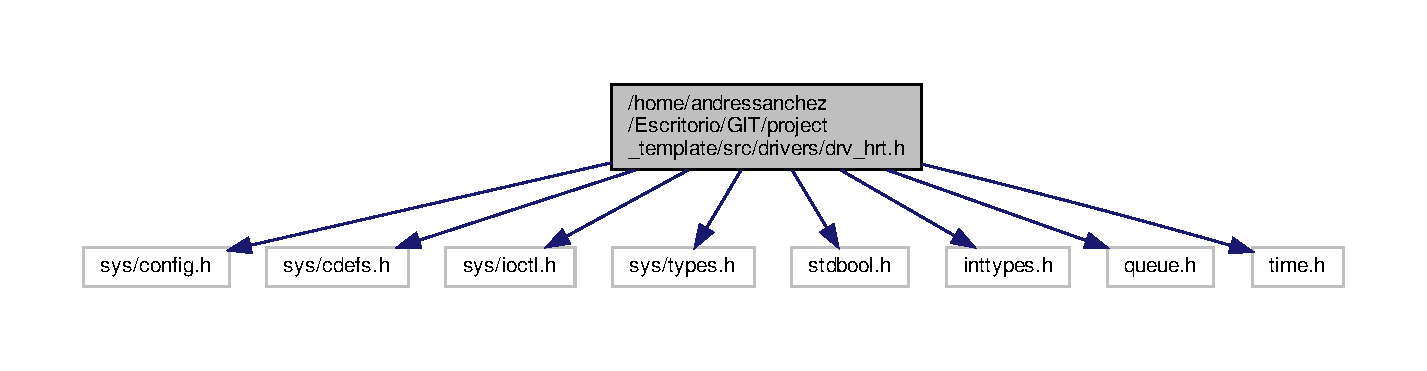
\includegraphics[width=350pt]{d2/d2a/drv__hrt_8h__incl}
\end{center}
\end{figure}
This graph shows which files directly or indirectly include this file\+:
\nopagebreak
\begin{figure}[H]
\begin{center}
\leavevmode
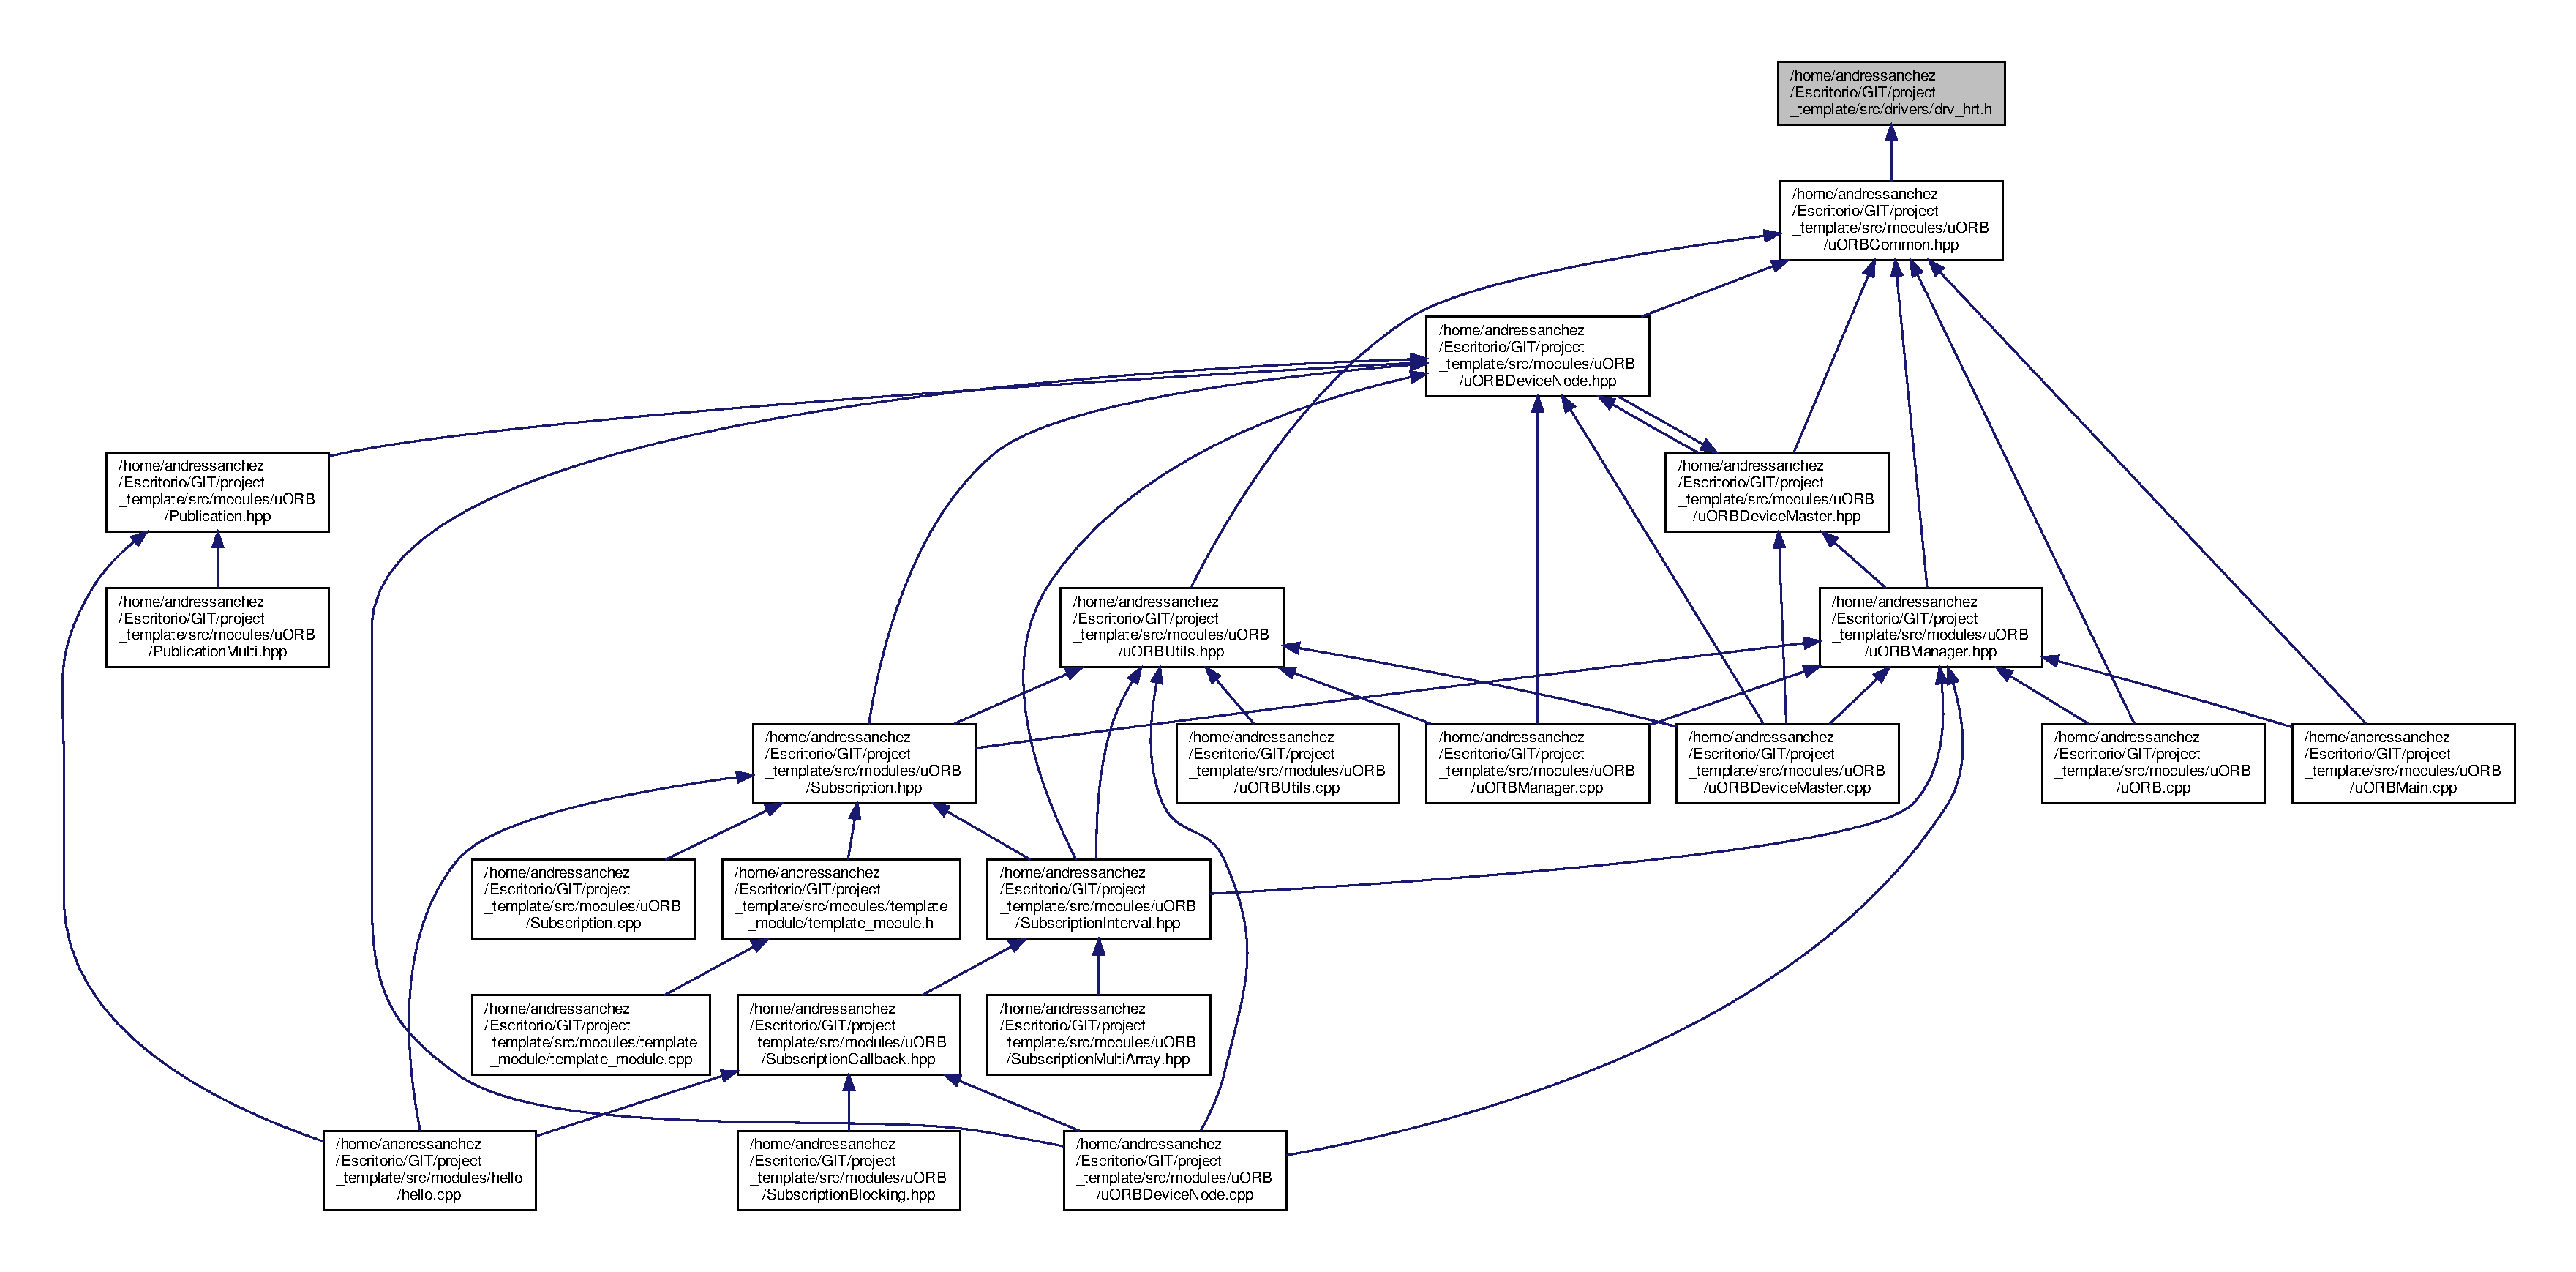
\includegraphics[width=350pt]{de/d15/drv__hrt_8h__dep__incl}
\end{center}
\end{figure}
\subsection*{Classes}
\begin{DoxyCompactItemize}
\item 
struct \hyperlink{structhrt__call}{hrt\+\_\+call}
\end{DoxyCompactItemize}
\subsection*{Macros}
\begin{DoxyCompactItemize}
\item 
\mbox{\Hypertarget{drv__hrt_8h_ae5a15cd41d77deeacec97b9d80730ff1}\label{drv__hrt_8h_ae5a15cd41d77deeacec97b9d80730ff1}} 
\#define {\bfseries L\+A\+T\+E\+N\+C\+Y\+\_\+\+B\+U\+C\+K\+E\+T\+\_\+\+C\+O\+U\+NT}~8
\end{DoxyCompactItemize}
\subsection*{Typedefs}
\begin{DoxyCompactItemize}
\item 
typedef void($\ast$ \hyperlink{drv__hrt_8h_ac8f5a61245c186b72dbbd2466dcceea5}{hrt\+\_\+callout}) (void $\ast$arg)
\item 
typedef struct \hyperlink{structhrt__call}{hrt\+\_\+call} $\ast$ \hyperlink{drv__hrt_8h_af2ddabce5b3a99b99716c0fb99fafaf5}{hrt\+\_\+call\+\_\+t}
\end{DoxyCompactItemize}
\subsection*{Functions}
\begin{DoxyCompactItemize}
\item 
\+\_\+\+\_\+\+E\+X\+P\+O\+RT void \hyperlink{drv__hrt_8h_a50cc6ecc5e8e0d6bfba0c3968d981284}{abstime\+\_\+to\+\_\+ts} (struct timespec $\ast$ts, \hyperlink{drv__hrt_8h_a9f8bbf0e883115e04a457a268533a87c}{hrt\+\_\+abstime} abstime)
\item 
\hyperlink{drv__hrt_8h_a9f8bbf0e883115e04a457a268533a87c}{hrt\+\_\+abstime} \hyperlink{drv__hrt_8h_a583009876e7b978d4ce681a0fe4c9aaf}{ts\+\_\+to\+\_\+abstime} (const struct timespec $\ast$ts)
\item 
\hyperlink{drv__hrt_8h_a9f8bbf0e883115e04a457a268533a87c}{hrt\+\_\+abstime} \hyperlink{drv__hrt_8h_a91f4291796ed7fbe544dc22ee5288367}{hrt\+\_\+absolute\+\_\+time} (void)
\item 
\+\_\+\+\_\+\+E\+X\+P\+O\+RT \hyperlink{drv__hrt_8h_a9f8bbf0e883115e04a457a268533a87c}{hrt\+\_\+abstime} \hyperlink{drv__hrt_8h_a721dee0a94d421de75e4836aed05c0b8}{hrt\+\_\+elapsed\+\_\+time\+\_\+atomic} (const volatile \hyperlink{drv__hrt_8h_a9f8bbf0e883115e04a457a268533a87c}{hrt\+\_\+abstime} $\ast$then)
\item 
\+\_\+\+\_\+\+E\+X\+P\+O\+RT void \hyperlink{drv__hrt_8h_a1a3d27d3fcc825c7dc7624a533c1a0c4}{hrt\+\_\+store\+\_\+absolute\+\_\+time} (volatile \hyperlink{drv__hrt_8h_a9f8bbf0e883115e04a457a268533a87c}{hrt\+\_\+abstime} $\ast$time)
\item 
\+\_\+\+\_\+\+E\+X\+P\+O\+RT void \hyperlink{drv__hrt_8h_a185fdd7c4d51c3f7ef22133ef56f9a55}{hrt\+\_\+call\+\_\+after} (struct \hyperlink{structhrt__call}{hrt\+\_\+call} $\ast$entry, \hyperlink{drv__hrt_8h_a9f8bbf0e883115e04a457a268533a87c}{hrt\+\_\+abstime} delay, \hyperlink{drv__hrt_8h_ac8f5a61245c186b72dbbd2466dcceea5}{hrt\+\_\+callout} callout, void $\ast$arg)
\item 
\+\_\+\+\_\+\+E\+X\+P\+O\+RT void \hyperlink{drv__hrt_8h_a7d49af6c126c7e49c903e2e47e70d716}{hrt\+\_\+call\+\_\+at} (struct \hyperlink{structhrt__call}{hrt\+\_\+call} $\ast$entry, \hyperlink{drv__hrt_8h_a9f8bbf0e883115e04a457a268533a87c}{hrt\+\_\+abstime} calltime, \hyperlink{drv__hrt_8h_ac8f5a61245c186b72dbbd2466dcceea5}{hrt\+\_\+callout} callout, void $\ast$arg)
\item 
\+\_\+\+\_\+\+E\+X\+P\+O\+RT void \hyperlink{drv__hrt_8h_afef961eed389b142649f3d904df16cd2}{hrt\+\_\+call\+\_\+every} (struct \hyperlink{structhrt__call}{hrt\+\_\+call} $\ast$entry, \hyperlink{drv__hrt_8h_a9f8bbf0e883115e04a457a268533a87c}{hrt\+\_\+abstime} delay, \hyperlink{drv__hrt_8h_a9f8bbf0e883115e04a457a268533a87c}{hrt\+\_\+abstime} interval, \hyperlink{drv__hrt_8h_ac8f5a61245c186b72dbbd2466dcceea5}{hrt\+\_\+callout} callout, void $\ast$arg)
\item 
\+\_\+\+\_\+\+E\+X\+P\+O\+RT bool \hyperlink{drv__hrt_8h_a384e9e9c38310512247c86560adb0b6d}{hrt\+\_\+called} (struct \hyperlink{structhrt__call}{hrt\+\_\+call} $\ast$entry)
\item 
\+\_\+\+\_\+\+E\+X\+P\+O\+RT void \hyperlink{drv__hrt_8h_aa4f22acddbadeed844ef6329629d2837}{hrt\+\_\+cancel} (struct \hyperlink{structhrt__call}{hrt\+\_\+call} $\ast$entry)
\item 
\+\_\+\+\_\+\+E\+X\+P\+O\+RT void \hyperlink{drv__hrt_8h_a0d90b23c796be1ed96cc58db0a38046d}{hrt\+\_\+call\+\_\+init} (struct \hyperlink{structhrt__call}{hrt\+\_\+call} $\ast$entry)
\item 
\mbox{\Hypertarget{drv__hrt_8h_a2c90bdef11ab9384cde0fa4c080ec697}\label{drv__hrt_8h_a2c90bdef11ab9384cde0fa4c080ec697}} 
\+\_\+\+\_\+\+E\+X\+P\+O\+RT void {\bfseries hrt\+\_\+call\+\_\+delay} (struct \hyperlink{structhrt__call}{hrt\+\_\+call} $\ast$entry, \hyperlink{drv__hrt_8h_a9f8bbf0e883115e04a457a268533a87c}{hrt\+\_\+abstime} delay)
\item 
\mbox{\Hypertarget{drv__hrt_8h_a4d623c5e3d99e6855ac85e606bd87e1c}\label{drv__hrt_8h_a4d623c5e3d99e6855ac85e606bd87e1c}} 
\+\_\+\+\_\+\+E\+X\+P\+O\+RT void {\bfseries hrt\+\_\+init} (void)
\end{DoxyCompactItemize}
\subsection*{Variables}
\begin{DoxyCompactItemize}
\item 
\+\_\+\+\_\+\+B\+E\+G\+I\+N\+\_\+\+D\+E\+C\+LS typedef uint64\+\_\+t \hyperlink{drv__hrt_8h_a9f8bbf0e883115e04a457a268533a87c}{hrt\+\_\+abstime}
\item 
\mbox{\Hypertarget{drv__hrt_8h_ae151daeebc72434d6551f9fe31f3327e}\label{drv__hrt_8h_ae151daeebc72434d6551f9fe31f3327e}} 
const uint16\+\_\+t {\bfseries latency\+\_\+bucket\+\_\+count}
\item 
\mbox{\Hypertarget{drv__hrt_8h_abde1b873868499addf6db659de1f79f1}\label{drv__hrt_8h_abde1b873868499addf6db659de1f79f1}} 
const uint16\+\_\+t {\bfseries latency\+\_\+buckets} \mbox{[}L\+A\+T\+E\+N\+C\+Y\+\_\+\+B\+U\+C\+K\+E\+T\+\_\+\+C\+O\+U\+NT\mbox{]}
\item 
\mbox{\Hypertarget{drv__hrt_8h_a026b1f9068d4be899ed439a5f66bcb6d}\label{drv__hrt_8h_a026b1f9068d4be899ed439a5f66bcb6d}} 
uint32\+\_\+t {\bfseries latency\+\_\+counters} \mbox{[}L\+A\+T\+E\+N\+C\+Y\+\_\+\+B\+U\+C\+K\+E\+T\+\_\+\+C\+O\+U\+NT+1\mbox{]}
\end{DoxyCompactItemize}


\subsection{Detailed Description}
High-\/resolution timer with callouts and timekeeping. 

\subsection{Typedef Documentation}
\mbox{\Hypertarget{drv__hrt_8h_af2ddabce5b3a99b99716c0fb99fafaf5}\label{drv__hrt_8h_af2ddabce5b3a99b99716c0fb99fafaf5}} 
\index{drv\+\_\+hrt.\+h@{drv\+\_\+hrt.\+h}!hrt\+\_\+call\+\_\+t@{hrt\+\_\+call\+\_\+t}}
\index{hrt\+\_\+call\+\_\+t@{hrt\+\_\+call\+\_\+t}!drv\+\_\+hrt.\+h@{drv\+\_\+hrt.\+h}}
\subsubsection{\texorpdfstring{hrt\+\_\+call\+\_\+t}{hrt\_call\_t}}
{\footnotesize\ttfamily typedef struct \hyperlink{structhrt__call}{hrt\+\_\+call} $\ast$ \hyperlink{drv__hrt_8h_af2ddabce5b3a99b99716c0fb99fafaf5}{hrt\+\_\+call\+\_\+t}}

Callout record. \mbox{\Hypertarget{drv__hrt_8h_ac8f5a61245c186b72dbbd2466dcceea5}\label{drv__hrt_8h_ac8f5a61245c186b72dbbd2466dcceea5}} 
\index{drv\+\_\+hrt.\+h@{drv\+\_\+hrt.\+h}!hrt\+\_\+callout@{hrt\+\_\+callout}}
\index{hrt\+\_\+callout@{hrt\+\_\+callout}!drv\+\_\+hrt.\+h@{drv\+\_\+hrt.\+h}}
\subsubsection{\texorpdfstring{hrt\+\_\+callout}{hrt\_callout}}
{\footnotesize\ttfamily typedef void($\ast$  hrt\+\_\+callout) (void $\ast$arg)}

Callout function type.

Note that callouts run in the timer interrupt context, so they are serialised with respect to each other, and must not block. 

Definition at line 75 of file drv\+\_\+hrt.\+h.



\subsection{Function Documentation}
\mbox{\Hypertarget{drv__hrt_8h_a50cc6ecc5e8e0d6bfba0c3968d981284}\label{drv__hrt_8h_a50cc6ecc5e8e0d6bfba0c3968d981284}} 
\index{drv\+\_\+hrt.\+h@{drv\+\_\+hrt.\+h}!abstime\+\_\+to\+\_\+ts@{abstime\+\_\+to\+\_\+ts}}
\index{abstime\+\_\+to\+\_\+ts@{abstime\+\_\+to\+\_\+ts}!drv\+\_\+hrt.\+h@{drv\+\_\+hrt.\+h}}
\subsubsection{\texorpdfstring{abstime\+\_\+to\+\_\+ts()}{abstime\_to\_ts()}}
{\footnotesize\ttfamily \+\_\+\+\_\+\+E\+X\+P\+O\+RT void abstime\+\_\+to\+\_\+ts (\begin{DoxyParamCaption}\item[{struct timespec $\ast$}]{ts,  }\item[{\hyperlink{drv__hrt_8h_a9f8bbf0e883115e04a457a268533a87c}{hrt\+\_\+abstime}}]{abstime }\end{DoxyParamCaption})}

Convert absolute time to a timespec. \mbox{\Hypertarget{drv__hrt_8h_a91f4291796ed7fbe544dc22ee5288367}\label{drv__hrt_8h_a91f4291796ed7fbe544dc22ee5288367}} 
\index{drv\+\_\+hrt.\+h@{drv\+\_\+hrt.\+h}!hrt\+\_\+absolute\+\_\+time@{hrt\+\_\+absolute\+\_\+time}}
\index{hrt\+\_\+absolute\+\_\+time@{hrt\+\_\+absolute\+\_\+time}!drv\+\_\+hrt.\+h@{drv\+\_\+hrt.\+h}}
\subsubsection{\texorpdfstring{hrt\+\_\+absolute\+\_\+time()}{hrt\_absolute\_time()}}
{\footnotesize\ttfamily \hyperlink{drv__hrt_8h_a9f8bbf0e883115e04a457a268533a87c}{hrt\+\_\+abstime} hrt\+\_\+absolute\+\_\+time (\begin{DoxyParamCaption}\item[{void}]{ }\end{DoxyParamCaption})\hspace{0.3cm}{\ttfamily [inline]}}

Get absolute time in \mbox{[}us\mbox{]} (does not wrap). 

Definition at line 118 of file drv\+\_\+hrt.\+h.


\begin{DoxyCode}
119 \{
120     \textcolor{keyword}{struct }timespec time;
121     clock\_gettime(CLOCK\_MONOTONIC, &time);
122     \hyperlink{drv__hrt_8h_a9f8bbf0e883115e04a457a268533a87c}{hrt\_abstime} now = \hyperlink{drv__hrt_8h_a583009876e7b978d4ce681a0fe4c9aaf}{ts\_to\_abstime}(&time);
123     \textcolor{keywordflow}{return} now;
124 \}
\end{DoxyCode}
\mbox{\Hypertarget{drv__hrt_8h_a185fdd7c4d51c3f7ef22133ef56f9a55}\label{drv__hrt_8h_a185fdd7c4d51c3f7ef22133ef56f9a55}} 
\index{drv\+\_\+hrt.\+h@{drv\+\_\+hrt.\+h}!hrt\+\_\+call\+\_\+after@{hrt\+\_\+call\+\_\+after}}
\index{hrt\+\_\+call\+\_\+after@{hrt\+\_\+call\+\_\+after}!drv\+\_\+hrt.\+h@{drv\+\_\+hrt.\+h}}
\subsubsection{\texorpdfstring{hrt\+\_\+call\+\_\+after()}{hrt\_call\_after()}}
{\footnotesize\ttfamily \+\_\+\+\_\+\+E\+X\+P\+O\+RT void hrt\+\_\+call\+\_\+after (\begin{DoxyParamCaption}\item[{struct \hyperlink{structhrt__call}{hrt\+\_\+call} $\ast$}]{entry,  }\item[{\hyperlink{drv__hrt_8h_a9f8bbf0e883115e04a457a268533a87c}{hrt\+\_\+abstime}}]{delay,  }\item[{\hyperlink{drv__hrt_8h_ac8f5a61245c186b72dbbd2466dcceea5}{hrt\+\_\+callout}}]{callout,  }\item[{void $\ast$}]{arg }\end{DoxyParamCaption})}

Call callout(arg) after delay has elapsed.

If callout is N\+U\+LL, this can be used to implement a timeout by testing the call with \hyperlink{drv__hrt_8h_a384e9e9c38310512247c86560adb0b6d}{hrt\+\_\+called()}. \mbox{\Hypertarget{drv__hrt_8h_a7d49af6c126c7e49c903e2e47e70d716}\label{drv__hrt_8h_a7d49af6c126c7e49c903e2e47e70d716}} 
\index{drv\+\_\+hrt.\+h@{drv\+\_\+hrt.\+h}!hrt\+\_\+call\+\_\+at@{hrt\+\_\+call\+\_\+at}}
\index{hrt\+\_\+call\+\_\+at@{hrt\+\_\+call\+\_\+at}!drv\+\_\+hrt.\+h@{drv\+\_\+hrt.\+h}}
\subsubsection{\texorpdfstring{hrt\+\_\+call\+\_\+at()}{hrt\_call\_at()}}
{\footnotesize\ttfamily \+\_\+\+\_\+\+E\+X\+P\+O\+RT void hrt\+\_\+call\+\_\+at (\begin{DoxyParamCaption}\item[{struct \hyperlink{structhrt__call}{hrt\+\_\+call} $\ast$}]{entry,  }\item[{\hyperlink{drv__hrt_8h_a9f8bbf0e883115e04a457a268533a87c}{hrt\+\_\+abstime}}]{calltime,  }\item[{\hyperlink{drv__hrt_8h_ac8f5a61245c186b72dbbd2466dcceea5}{hrt\+\_\+callout}}]{callout,  }\item[{void $\ast$}]{arg }\end{DoxyParamCaption})}

Call callout(arg) at absolute time calltime. \mbox{\Hypertarget{drv__hrt_8h_afef961eed389b142649f3d904df16cd2}\label{drv__hrt_8h_afef961eed389b142649f3d904df16cd2}} 
\index{drv\+\_\+hrt.\+h@{drv\+\_\+hrt.\+h}!hrt\+\_\+call\+\_\+every@{hrt\+\_\+call\+\_\+every}}
\index{hrt\+\_\+call\+\_\+every@{hrt\+\_\+call\+\_\+every}!drv\+\_\+hrt.\+h@{drv\+\_\+hrt.\+h}}
\subsubsection{\texorpdfstring{hrt\+\_\+call\+\_\+every()}{hrt\_call\_every()}}
{\footnotesize\ttfamily \+\_\+\+\_\+\+E\+X\+P\+O\+RT void hrt\+\_\+call\+\_\+every (\begin{DoxyParamCaption}\item[{struct \hyperlink{structhrt__call}{hrt\+\_\+call} $\ast$}]{entry,  }\item[{\hyperlink{drv__hrt_8h_a9f8bbf0e883115e04a457a268533a87c}{hrt\+\_\+abstime}}]{delay,  }\item[{\hyperlink{drv__hrt_8h_a9f8bbf0e883115e04a457a268533a87c}{hrt\+\_\+abstime}}]{interval,  }\item[{\hyperlink{drv__hrt_8h_ac8f5a61245c186b72dbbd2466dcceea5}{hrt\+\_\+callout}}]{callout,  }\item[{void $\ast$}]{arg }\end{DoxyParamCaption})}

Call callout(arg) after delay, and then after every interval.

Note thet the interval is timed between scheduled, not actual, call times, so the call rate may jitter but should not drift. \mbox{\Hypertarget{drv__hrt_8h_a0d90b23c796be1ed96cc58db0a38046d}\label{drv__hrt_8h_a0d90b23c796be1ed96cc58db0a38046d}} 
\index{drv\+\_\+hrt.\+h@{drv\+\_\+hrt.\+h}!hrt\+\_\+call\+\_\+init@{hrt\+\_\+call\+\_\+init}}
\index{hrt\+\_\+call\+\_\+init@{hrt\+\_\+call\+\_\+init}!drv\+\_\+hrt.\+h@{drv\+\_\+hrt.\+h}}
\subsubsection{\texorpdfstring{hrt\+\_\+call\+\_\+init()}{hrt\_call\_init()}}
{\footnotesize\ttfamily \+\_\+\+\_\+\+E\+X\+P\+O\+RT void hrt\+\_\+call\+\_\+init (\begin{DoxyParamCaption}\item[{struct \hyperlink{structhrt__call}{hrt\+\_\+call} $\ast$}]{entry }\end{DoxyParamCaption})}

Initialise a \hyperlink{structhrt__call}{hrt\+\_\+call} structure \mbox{\Hypertarget{drv__hrt_8h_a384e9e9c38310512247c86560adb0b6d}\label{drv__hrt_8h_a384e9e9c38310512247c86560adb0b6d}} 
\index{drv\+\_\+hrt.\+h@{drv\+\_\+hrt.\+h}!hrt\+\_\+called@{hrt\+\_\+called}}
\index{hrt\+\_\+called@{hrt\+\_\+called}!drv\+\_\+hrt.\+h@{drv\+\_\+hrt.\+h}}
\subsubsection{\texorpdfstring{hrt\+\_\+called()}{hrt\_called()}}
{\footnotesize\ttfamily \+\_\+\+\_\+\+E\+X\+P\+O\+RT bool hrt\+\_\+called (\begin{DoxyParamCaption}\item[{struct \hyperlink{structhrt__call}{hrt\+\_\+call} $\ast$}]{entry }\end{DoxyParamCaption})}

If this returns true, the entry has been invoked and removed from the callout list, or it has never been entered.

Always returns false for repeating callouts. \mbox{\Hypertarget{drv__hrt_8h_aa4f22acddbadeed844ef6329629d2837}\label{drv__hrt_8h_aa4f22acddbadeed844ef6329629d2837}} 
\index{drv\+\_\+hrt.\+h@{drv\+\_\+hrt.\+h}!hrt\+\_\+cancel@{hrt\+\_\+cancel}}
\index{hrt\+\_\+cancel@{hrt\+\_\+cancel}!drv\+\_\+hrt.\+h@{drv\+\_\+hrt.\+h}}
\subsubsection{\texorpdfstring{hrt\+\_\+cancel()}{hrt\_cancel()}}
{\footnotesize\ttfamily \+\_\+\+\_\+\+E\+X\+P\+O\+RT void hrt\+\_\+cancel (\begin{DoxyParamCaption}\item[{struct \hyperlink{structhrt__call}{hrt\+\_\+call} $\ast$}]{entry }\end{DoxyParamCaption})}

Remove the entry from the callout list. \mbox{\Hypertarget{drv__hrt_8h_a721dee0a94d421de75e4836aed05c0b8}\label{drv__hrt_8h_a721dee0a94d421de75e4836aed05c0b8}} 
\index{drv\+\_\+hrt.\+h@{drv\+\_\+hrt.\+h}!hrt\+\_\+elapsed\+\_\+time\+\_\+atomic@{hrt\+\_\+elapsed\+\_\+time\+\_\+atomic}}
\index{hrt\+\_\+elapsed\+\_\+time\+\_\+atomic@{hrt\+\_\+elapsed\+\_\+time\+\_\+atomic}!drv\+\_\+hrt.\+h@{drv\+\_\+hrt.\+h}}
\subsubsection{\texorpdfstring{hrt\+\_\+elapsed\+\_\+time\+\_\+atomic()}{hrt\_elapsed\_time\_atomic()}}
{\footnotesize\ttfamily \+\_\+\+\_\+\+E\+X\+P\+O\+RT \hyperlink{drv__hrt_8h_a9f8bbf0e883115e04a457a268533a87c}{hrt\+\_\+abstime} hrt\+\_\+elapsed\+\_\+time\+\_\+atomic (\begin{DoxyParamCaption}\item[{const volatile \hyperlink{drv__hrt_8h_a9f8bbf0e883115e04a457a268533a87c}{hrt\+\_\+abstime} $\ast$}]{then }\end{DoxyParamCaption})}

Compute the delta between a timestamp taken in the past and now.

This function is safe to use even if the timestamp is updated by an interrupt during execution. \mbox{\Hypertarget{drv__hrt_8h_a1a3d27d3fcc825c7dc7624a533c1a0c4}\label{drv__hrt_8h_a1a3d27d3fcc825c7dc7624a533c1a0c4}} 
\index{drv\+\_\+hrt.\+h@{drv\+\_\+hrt.\+h}!hrt\+\_\+store\+\_\+absolute\+\_\+time@{hrt\+\_\+store\+\_\+absolute\+\_\+time}}
\index{hrt\+\_\+store\+\_\+absolute\+\_\+time@{hrt\+\_\+store\+\_\+absolute\+\_\+time}!drv\+\_\+hrt.\+h@{drv\+\_\+hrt.\+h}}
\subsubsection{\texorpdfstring{hrt\+\_\+store\+\_\+absolute\+\_\+time()}{hrt\_store\_absolute\_time()}}
{\footnotesize\ttfamily \+\_\+\+\_\+\+E\+X\+P\+O\+RT void hrt\+\_\+store\+\_\+absolute\+\_\+time (\begin{DoxyParamCaption}\item[{volatile \hyperlink{drv__hrt_8h_a9f8bbf0e883115e04a457a268533a87c}{hrt\+\_\+abstime} $\ast$}]{time }\end{DoxyParamCaption})}

Store the absolute time in an interrupt-\/safe fashion.

This function ensures that the timestamp cannot be seen half-\/written by an interrupt handler. \mbox{\Hypertarget{drv__hrt_8h_a583009876e7b978d4ce681a0fe4c9aaf}\label{drv__hrt_8h_a583009876e7b978d4ce681a0fe4c9aaf}} 
\index{drv\+\_\+hrt.\+h@{drv\+\_\+hrt.\+h}!ts\+\_\+to\+\_\+abstime@{ts\+\_\+to\+\_\+abstime}}
\index{ts\+\_\+to\+\_\+abstime@{ts\+\_\+to\+\_\+abstime}!drv\+\_\+hrt.\+h@{drv\+\_\+hrt.\+h}}
\subsubsection{\texorpdfstring{ts\+\_\+to\+\_\+abstime()}{ts\_to\_abstime()}}
{\footnotesize\ttfamily \hyperlink{drv__hrt_8h_a9f8bbf0e883115e04a457a268533a87c}{hrt\+\_\+abstime} ts\+\_\+to\+\_\+abstime (\begin{DoxyParamCaption}\item[{const struct timespec $\ast$}]{ts }\end{DoxyParamCaption})\hspace{0.3cm}{\ttfamily [inline]}}

Convert absolute time to a timespec. 

Definition at line 105 of file drv\+\_\+hrt.\+h.


\begin{DoxyCode}
106 \{
107     \hyperlink{drv__hrt_8h_a9f8bbf0e883115e04a457a268533a87c}{hrt\_abstime}  result;
108 
109     result = (\hyperlink{drv__hrt_8h_a9f8bbf0e883115e04a457a268533a87c}{hrt\_abstime})(ts->tv\_sec) * 1000000;
110     result += ts->tv\_nsec / 1000;
111 
112     \textcolor{keywordflow}{return} result;
113 \}
\end{DoxyCode}


\subsection{Variable Documentation}
\mbox{\Hypertarget{drv__hrt_8h_a9f8bbf0e883115e04a457a268533a87c}\label{drv__hrt_8h_a9f8bbf0e883115e04a457a268533a87c}} 
\index{drv\+\_\+hrt.\+h@{drv\+\_\+hrt.\+h}!hrt\+\_\+abstime@{hrt\+\_\+abstime}}
\index{hrt\+\_\+abstime@{hrt\+\_\+abstime}!drv\+\_\+hrt.\+h@{drv\+\_\+hrt.\+h}}
\subsubsection{\texorpdfstring{hrt\+\_\+abstime}{hrt\_abstime}}
{\footnotesize\ttfamily \+\_\+\+\_\+\+B\+E\+G\+I\+N\+\_\+\+D\+E\+C\+LS typedef uint64\+\_\+t hrt\+\_\+abstime}

Absolute time, in microsecond units.

Absolute time is measured from some arbitrary epoch shortly after system startup. It should never wrap or go backwards. 

Definition at line 66 of file drv\+\_\+hrt.\+h.


\hypertarget{drv__orb__dev_8h}{}\section{/home/andressanchez/\+Escritorio/\+G\+I\+T/project\+\_\+template/src/drivers/drv\+\_\+orb\+\_\+dev.h File Reference}
\label{drv__orb__dev_8h}\index{/home/andressanchez/\+Escritorio/\+G\+I\+T/project\+\_\+template/src/drivers/drv\+\_\+orb\+\_\+dev.\+h@{/home/andressanchez/\+Escritorio/\+G\+I\+T/project\+\_\+template/src/drivers/drv\+\_\+orb\+\_\+dev.\+h}}
{\ttfamily \#include $<$sys/types.\+h$>$}\newline
{\ttfamily \#include $<$sys/ioctl.\+h$>$}\newline
{\ttfamily \#include $<$stdint.\+h$>$}\newline
Include dependency graph for drv\+\_\+orb\+\_\+dev.\+h\+:\nopagebreak
\begin{figure}[H]
\begin{center}
\leavevmode
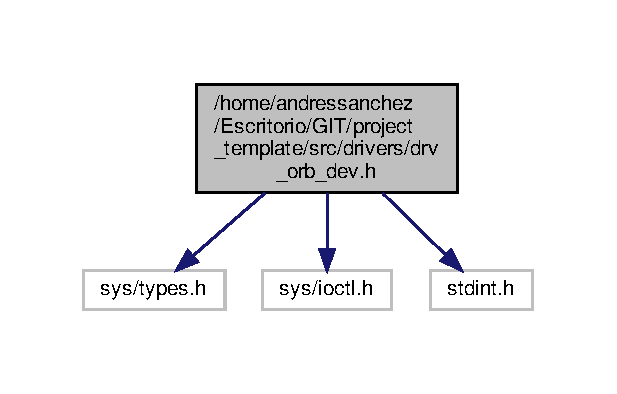
\includegraphics[width=296pt]{d6/d6f/drv__orb__dev_8h__incl}
\end{center}
\end{figure}
This graph shows which files directly or indirectly include this file\+:
\nopagebreak
\begin{figure}[H]
\begin{center}
\leavevmode
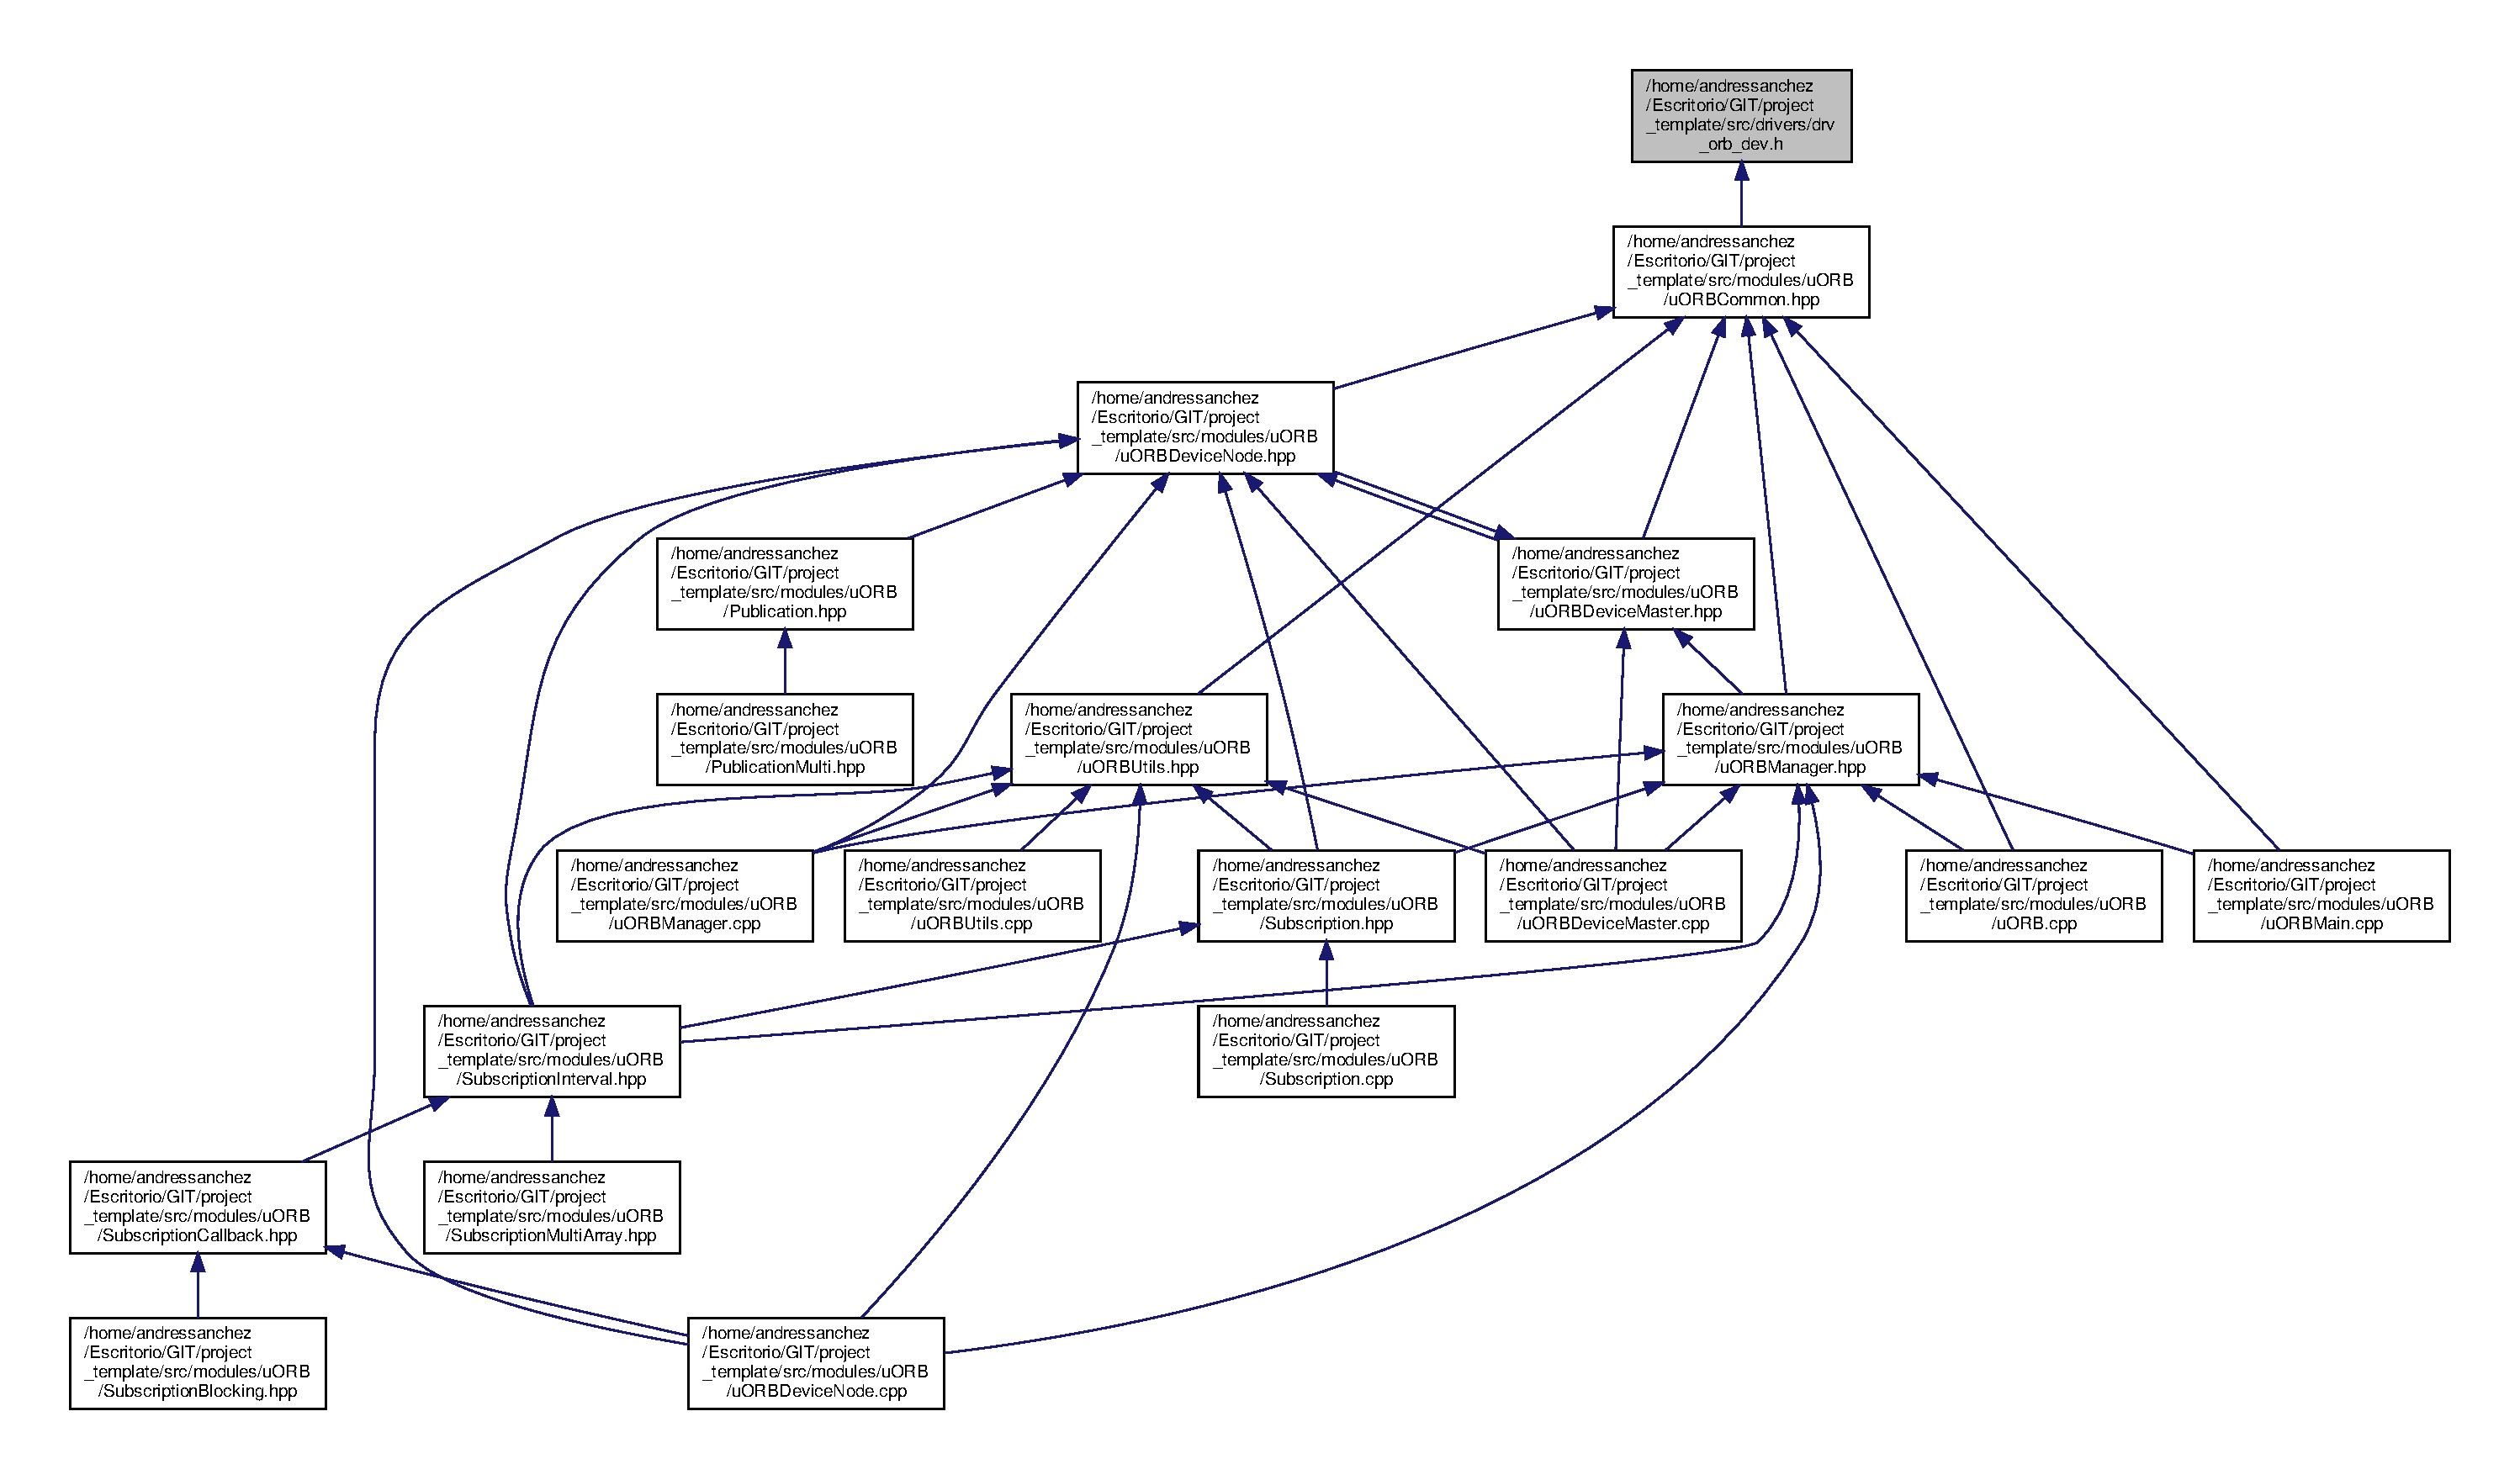
\includegraphics[width=350pt]{d1/dff/drv__orb__dev_8h__dep__incl}
\end{center}
\end{figure}
\subsection*{Macros}
\begin{DoxyCompactItemize}
\item 
\mbox{\Hypertarget{drv__orb__dev_8h_a7b32b0c4e23811707ad464118a47112d}\label{drv__orb__dev_8h_a7b32b0c4e23811707ad464118a47112d}} 
\#define {\bfseries \+\_\+\+O\+R\+B\+I\+O\+C\+B\+A\+SE}~(0x2600)
\item 
\mbox{\Hypertarget{drv__orb__dev_8h_a2d1a6a804120ff1ce1bbe00d09bc8ac9}\label{drv__orb__dev_8h_a2d1a6a804120ff1ce1bbe00d09bc8ac9}} 
\#define {\bfseries \+\_\+\+O\+R\+B\+I\+OC}(\+\_\+n)~(\+\_\+\+I\+OC(\+\_\+\+O\+R\+B\+I\+O\+C\+B\+A\+SE, \+\_\+n))
\item 
\#define \hyperlink{drv__orb__dev_8h_a60e19540d21f9a44e9157804121957f8}{O\+R\+B\+I\+O\+C\+U\+P\+D\+A\+T\+ED}~\+\_\+\+O\+R\+B\+I\+OC(11)
\item 
\#define \hyperlink{drv__orb__dev_8h_a815da46533c3937c84c1496218659d0b}{O\+R\+B\+I\+O\+C\+S\+E\+T\+I\+N\+T\+E\+R\+V\+AL}~\+\_\+\+O\+R\+B\+I\+OC(12)
\item 
\#define \hyperlink{drv__orb__dev_8h_a0ba7c1d8b06e6930ed9589dbebbc775a}{O\+R\+B\+I\+O\+C\+G\+A\+D\+V\+E\+R\+T\+I\+S\+ER}~\+\_\+\+O\+R\+B\+I\+OC(13)
\item 
\#define \hyperlink{drv__orb__dev_8h_ae86f989506db64622e49c03e6a8ae681}{O\+R\+B\+I\+O\+C\+G\+P\+R\+I\+O\+R\+I\+TY}~\+\_\+\+O\+R\+B\+I\+OC(14)
\item 
\#define \hyperlink{drv__orb__dev_8h_a4835f9286d5aac7a6b5e0a01661cbee7}{O\+R\+B\+I\+O\+C\+S\+E\+T\+Q\+U\+E\+U\+E\+S\+I\+ZE}~\+\_\+\+O\+R\+B\+I\+OC(15)
\item 
\#define \hyperlink{drv__orb__dev_8h_acdbdb0d6f9b8600498ffa2599dca742d}{O\+R\+B\+I\+O\+C\+G\+E\+T\+I\+N\+T\+E\+R\+V\+AL}~\+\_\+\+O\+R\+B\+I\+OC(16)
\item 
\#define \hyperlink{drv__orb__dev_8h_a00f4a4fca062412c74b581a041c43c7a}{O\+R\+B\+I\+O\+C\+I\+S\+A\+D\+V\+E\+R\+T\+I\+S\+ED}~\+\_\+\+O\+R\+B\+I\+OC(17)
\end{DoxyCompactItemize}


\subsection{Detailed Description}
u\+O\+RB published object driver. 

\subsection{Macro Definition Documentation}
\mbox{\Hypertarget{drv__orb__dev_8h_a0ba7c1d8b06e6930ed9589dbebbc775a}\label{drv__orb__dev_8h_a0ba7c1d8b06e6930ed9589dbebbc775a}} 
\index{drv\+\_\+orb\+\_\+dev.\+h@{drv\+\_\+orb\+\_\+dev.\+h}!O\+R\+B\+I\+O\+C\+G\+A\+D\+V\+E\+R\+T\+I\+S\+ER@{O\+R\+B\+I\+O\+C\+G\+A\+D\+V\+E\+R\+T\+I\+S\+ER}}
\index{O\+R\+B\+I\+O\+C\+G\+A\+D\+V\+E\+R\+T\+I\+S\+ER@{O\+R\+B\+I\+O\+C\+G\+A\+D\+V\+E\+R\+T\+I\+S\+ER}!drv\+\_\+orb\+\_\+dev.\+h@{drv\+\_\+orb\+\_\+dev.\+h}}
\subsubsection{\texorpdfstring{O\+R\+B\+I\+O\+C\+G\+A\+D\+V\+E\+R\+T\+I\+S\+ER}{ORBIOCGADVERTISER}}
{\footnotesize\ttfamily \#define O\+R\+B\+I\+O\+C\+G\+A\+D\+V\+E\+R\+T\+I\+S\+ER~\+\_\+\+O\+R\+B\+I\+OC(13)}

Get the global advertiser handle for the topic 

Definition at line 61 of file drv\+\_\+orb\+\_\+dev.\+h.

\mbox{\Hypertarget{drv__orb__dev_8h_acdbdb0d6f9b8600498ffa2599dca742d}\label{drv__orb__dev_8h_acdbdb0d6f9b8600498ffa2599dca742d}} 
\index{drv\+\_\+orb\+\_\+dev.\+h@{drv\+\_\+orb\+\_\+dev.\+h}!O\+R\+B\+I\+O\+C\+G\+E\+T\+I\+N\+T\+E\+R\+V\+AL@{O\+R\+B\+I\+O\+C\+G\+E\+T\+I\+N\+T\+E\+R\+V\+AL}}
\index{O\+R\+B\+I\+O\+C\+G\+E\+T\+I\+N\+T\+E\+R\+V\+AL@{O\+R\+B\+I\+O\+C\+G\+E\+T\+I\+N\+T\+E\+R\+V\+AL}!drv\+\_\+orb\+\_\+dev.\+h@{drv\+\_\+orb\+\_\+dev.\+h}}
\subsubsection{\texorpdfstring{O\+R\+B\+I\+O\+C\+G\+E\+T\+I\+N\+T\+E\+R\+V\+AL}{ORBIOCGETINTERVAL}}
{\footnotesize\ttfamily \#define O\+R\+B\+I\+O\+C\+G\+E\+T\+I\+N\+T\+E\+R\+V\+AL~\+\_\+\+O\+R\+B\+I\+OC(16)}

Get the minimum interval at which the topic can be seen to be updated for this subscription 

Definition at line 70 of file drv\+\_\+orb\+\_\+dev.\+h.

\mbox{\Hypertarget{drv__orb__dev_8h_ae86f989506db64622e49c03e6a8ae681}\label{drv__orb__dev_8h_ae86f989506db64622e49c03e6a8ae681}} 
\index{drv\+\_\+orb\+\_\+dev.\+h@{drv\+\_\+orb\+\_\+dev.\+h}!O\+R\+B\+I\+O\+C\+G\+P\+R\+I\+O\+R\+I\+TY@{O\+R\+B\+I\+O\+C\+G\+P\+R\+I\+O\+R\+I\+TY}}
\index{O\+R\+B\+I\+O\+C\+G\+P\+R\+I\+O\+R\+I\+TY@{O\+R\+B\+I\+O\+C\+G\+P\+R\+I\+O\+R\+I\+TY}!drv\+\_\+orb\+\_\+dev.\+h@{drv\+\_\+orb\+\_\+dev.\+h}}
\subsubsection{\texorpdfstring{O\+R\+B\+I\+O\+C\+G\+P\+R\+I\+O\+R\+I\+TY}{ORBIOCGPRIORITY}}
{\footnotesize\ttfamily \#define O\+R\+B\+I\+O\+C\+G\+P\+R\+I\+O\+R\+I\+TY~\+\_\+\+O\+R\+B\+I\+OC(14)}

Get the priority for the topic 

Definition at line 64 of file drv\+\_\+orb\+\_\+dev.\+h.

\mbox{\Hypertarget{drv__orb__dev_8h_a00f4a4fca062412c74b581a041c43c7a}\label{drv__orb__dev_8h_a00f4a4fca062412c74b581a041c43c7a}} 
\index{drv\+\_\+orb\+\_\+dev.\+h@{drv\+\_\+orb\+\_\+dev.\+h}!O\+R\+B\+I\+O\+C\+I\+S\+A\+D\+V\+E\+R\+T\+I\+S\+ED@{O\+R\+B\+I\+O\+C\+I\+S\+A\+D\+V\+E\+R\+T\+I\+S\+ED}}
\index{O\+R\+B\+I\+O\+C\+I\+S\+A\+D\+V\+E\+R\+T\+I\+S\+ED@{O\+R\+B\+I\+O\+C\+I\+S\+A\+D\+V\+E\+R\+T\+I\+S\+ED}!drv\+\_\+orb\+\_\+dev.\+h@{drv\+\_\+orb\+\_\+dev.\+h}}
\subsubsection{\texorpdfstring{O\+R\+B\+I\+O\+C\+I\+S\+A\+D\+V\+E\+R\+T\+I\+S\+ED}{ORBIOCISADVERTISED}}
{\footnotesize\ttfamily \#define O\+R\+B\+I\+O\+C\+I\+S\+A\+D\+V\+E\+R\+T\+I\+S\+ED~\+\_\+\+O\+R\+B\+I\+OC(17)}

Check whether the topic is advertised, sets $\ast$(unsigned long $\ast$)arg to 1 if advertised, 0 otherwise 

Definition at line 73 of file drv\+\_\+orb\+\_\+dev.\+h.

\mbox{\Hypertarget{drv__orb__dev_8h_a815da46533c3937c84c1496218659d0b}\label{drv__orb__dev_8h_a815da46533c3937c84c1496218659d0b}} 
\index{drv\+\_\+orb\+\_\+dev.\+h@{drv\+\_\+orb\+\_\+dev.\+h}!O\+R\+B\+I\+O\+C\+S\+E\+T\+I\+N\+T\+E\+R\+V\+AL@{O\+R\+B\+I\+O\+C\+S\+E\+T\+I\+N\+T\+E\+R\+V\+AL}}
\index{O\+R\+B\+I\+O\+C\+S\+E\+T\+I\+N\+T\+E\+R\+V\+AL@{O\+R\+B\+I\+O\+C\+S\+E\+T\+I\+N\+T\+E\+R\+V\+AL}!drv\+\_\+orb\+\_\+dev.\+h@{drv\+\_\+orb\+\_\+dev.\+h}}
\subsubsection{\texorpdfstring{O\+R\+B\+I\+O\+C\+S\+E\+T\+I\+N\+T\+E\+R\+V\+AL}{ORBIOCSETINTERVAL}}
{\footnotesize\ttfamily \#define O\+R\+B\+I\+O\+C\+S\+E\+T\+I\+N\+T\+E\+R\+V\+AL~\+\_\+\+O\+R\+B\+I\+OC(12)}

Set the minimum interval at which the topic can be seen to be updated for this subscription 

Definition at line 58 of file drv\+\_\+orb\+\_\+dev.\+h.

\mbox{\Hypertarget{drv__orb__dev_8h_a4835f9286d5aac7a6b5e0a01661cbee7}\label{drv__orb__dev_8h_a4835f9286d5aac7a6b5e0a01661cbee7}} 
\index{drv\+\_\+orb\+\_\+dev.\+h@{drv\+\_\+orb\+\_\+dev.\+h}!O\+R\+B\+I\+O\+C\+S\+E\+T\+Q\+U\+E\+U\+E\+S\+I\+ZE@{O\+R\+B\+I\+O\+C\+S\+E\+T\+Q\+U\+E\+U\+E\+S\+I\+ZE}}
\index{O\+R\+B\+I\+O\+C\+S\+E\+T\+Q\+U\+E\+U\+E\+S\+I\+ZE@{O\+R\+B\+I\+O\+C\+S\+E\+T\+Q\+U\+E\+U\+E\+S\+I\+ZE}!drv\+\_\+orb\+\_\+dev.\+h@{drv\+\_\+orb\+\_\+dev.\+h}}
\subsubsection{\texorpdfstring{O\+R\+B\+I\+O\+C\+S\+E\+T\+Q\+U\+E\+U\+E\+S\+I\+ZE}{ORBIOCSETQUEUESIZE}}
{\footnotesize\ttfamily \#define O\+R\+B\+I\+O\+C\+S\+E\+T\+Q\+U\+E\+U\+E\+S\+I\+ZE~\+\_\+\+O\+R\+B\+I\+OC(15)}

Set the queue size of the topic 

Definition at line 67 of file drv\+\_\+orb\+\_\+dev.\+h.

\mbox{\Hypertarget{drv__orb__dev_8h_a60e19540d21f9a44e9157804121957f8}\label{drv__orb__dev_8h_a60e19540d21f9a44e9157804121957f8}} 
\index{drv\+\_\+orb\+\_\+dev.\+h@{drv\+\_\+orb\+\_\+dev.\+h}!O\+R\+B\+I\+O\+C\+U\+P\+D\+A\+T\+ED@{O\+R\+B\+I\+O\+C\+U\+P\+D\+A\+T\+ED}}
\index{O\+R\+B\+I\+O\+C\+U\+P\+D\+A\+T\+ED@{O\+R\+B\+I\+O\+C\+U\+P\+D\+A\+T\+ED}!drv\+\_\+orb\+\_\+dev.\+h@{drv\+\_\+orb\+\_\+dev.\+h}}
\subsubsection{\texorpdfstring{O\+R\+B\+I\+O\+C\+U\+P\+D\+A\+T\+ED}{ORBIOCUPDATED}}
{\footnotesize\ttfamily \#define O\+R\+B\+I\+O\+C\+U\+P\+D\+A\+T\+ED~\+\_\+\+O\+R\+B\+I\+OC(11)}

Check whether the topic has been updated since it was last read, sets $\ast$(bool $\ast$)arg 

Definition at line 55 of file drv\+\_\+orb\+\_\+dev.\+h.


\hypertarget{IntrusiveSortedList_8hpp}{}\section{/home/andressanchez/\+Escritorio/\+G\+I\+T/project\+\_\+template/src/include/containers/\+Intrusive\+Sorted\+List.hpp File Reference}
\label{IntrusiveSortedList_8hpp}\index{/home/andressanchez/\+Escritorio/\+G\+I\+T/project\+\_\+template/src/include/containers/\+Intrusive\+Sorted\+List.\+hpp@{/home/andressanchez/\+Escritorio/\+G\+I\+T/project\+\_\+template/src/include/containers/\+Intrusive\+Sorted\+List.\+hpp}}
{\ttfamily \#include $<$stdlib.\+h$>$}\newline
Include dependency graph for Intrusive\+Sorted\+List.\+hpp\+:\nopagebreak
\begin{figure}[H]
\begin{center}
\leavevmode
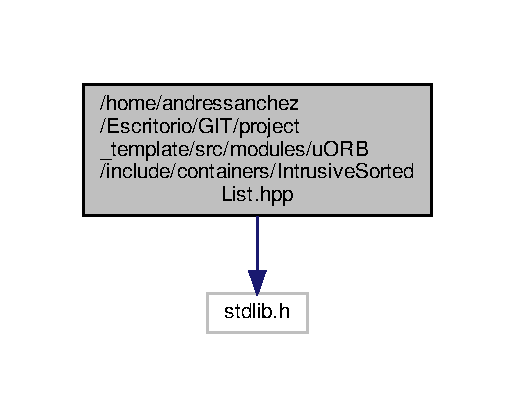
\includegraphics[width=238pt]{d2/d2a/IntrusiveSortedList_8hpp__incl}
\end{center}
\end{figure}
This graph shows which files directly or indirectly include this file\+:\nopagebreak
\begin{figure}[H]
\begin{center}
\leavevmode
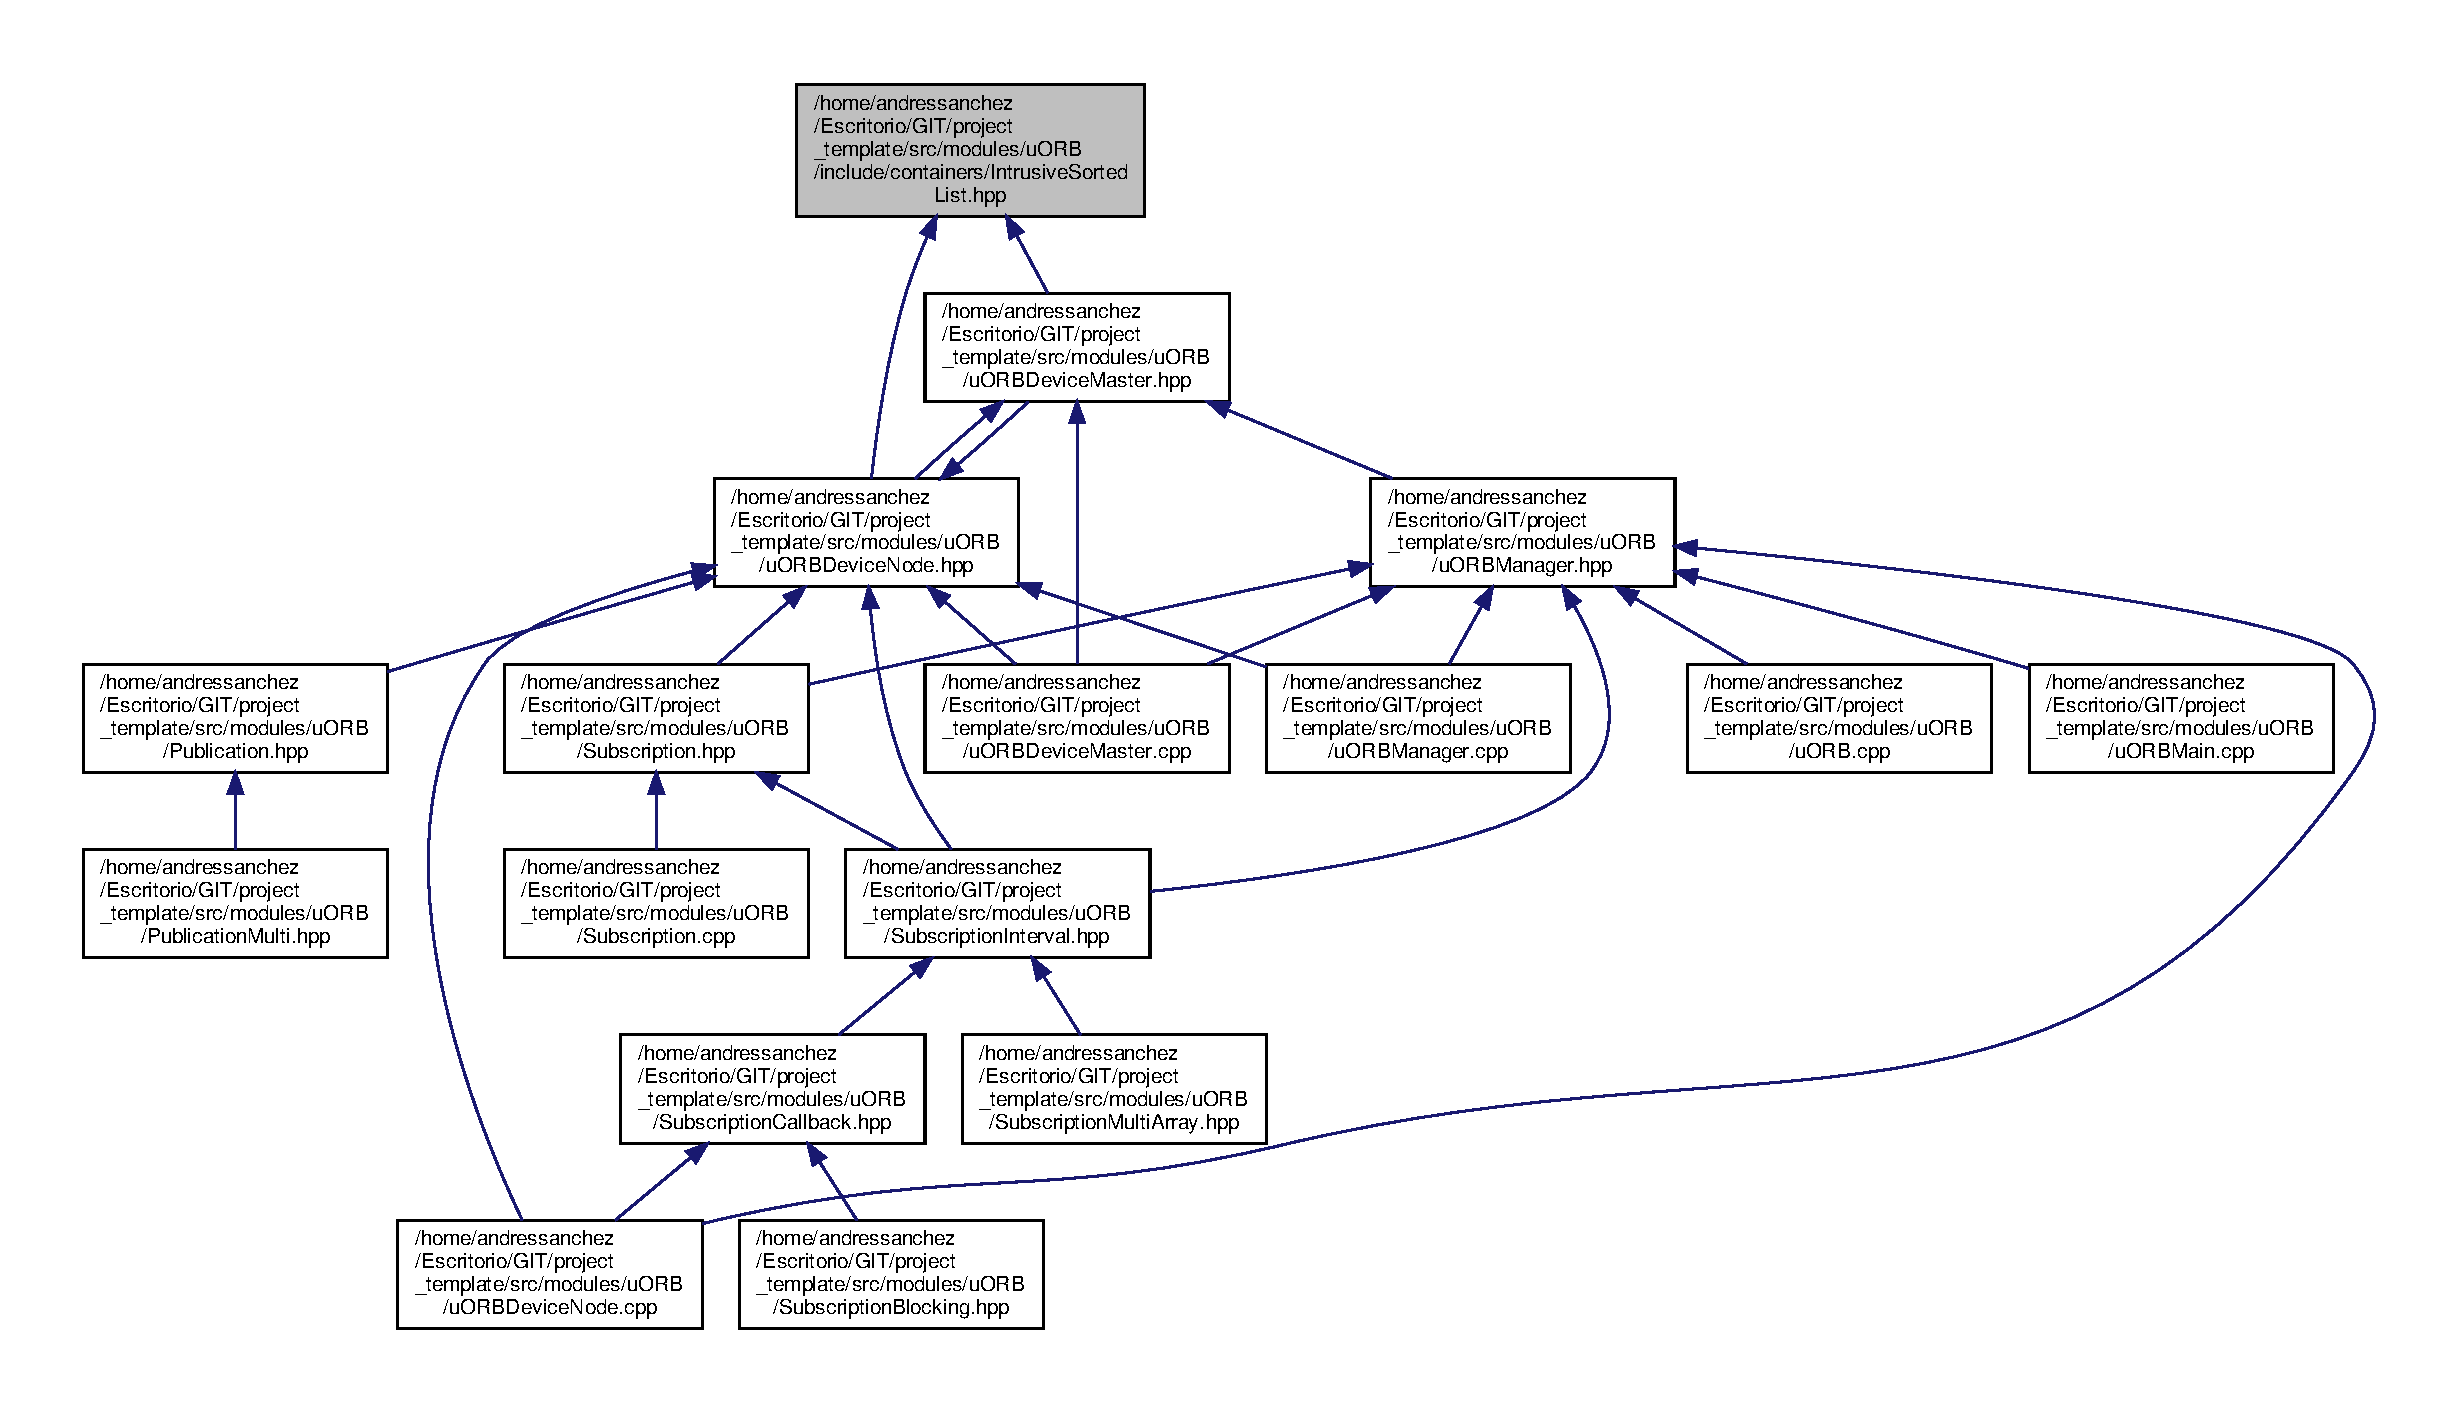
\includegraphics[width=350pt]{db/d44/IntrusiveSortedList_8hpp__dep__incl}
\end{center}
\end{figure}
\subsection*{Classes}
\begin{DoxyCompactItemize}
\item 
class \hyperlink{classIntrusiveSortedListNode}{Intrusive\+Sorted\+List\+Node$<$ T $>$}
\item 
class \hyperlink{classIntrusiveSortedList}{Intrusive\+Sorted\+List$<$ T $>$}
\item 
struct \hyperlink{structIntrusiveSortedList_1_1Iterator}{Intrusive\+Sorted\+List$<$ T $>$\+::\+Iterator}
\end{DoxyCompactItemize}


\subsection{Detailed Description}
An intrusive linked list where nodes are sorted on insertion. 
\hypertarget{List_8hpp}{}\section{/home/andressanchez/\+Escritorio/\+G\+I\+T/project\+\_\+template/src/include/containers/\+List.hpp File Reference}
\label{List_8hpp}\index{/home/andressanchez/\+Escritorio/\+G\+I\+T/project\+\_\+template/src/include/containers/\+List.\+hpp@{/home/andressanchez/\+Escritorio/\+G\+I\+T/project\+\_\+template/src/include/containers/\+List.\+hpp}}
{\ttfamily \#include $<$stdlib.\+h$>$}\newline
Include dependency graph for List.\+hpp\+:\nopagebreak
\begin{figure}[H]
\begin{center}
\leavevmode
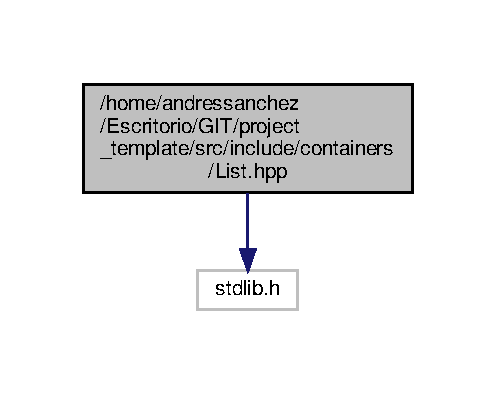
\includegraphics[width=238pt]{d7/de1/List_8hpp__incl}
\end{center}
\end{figure}
This graph shows which files directly or indirectly include this file\+:\nopagebreak
\begin{figure}[H]
\begin{center}
\leavevmode
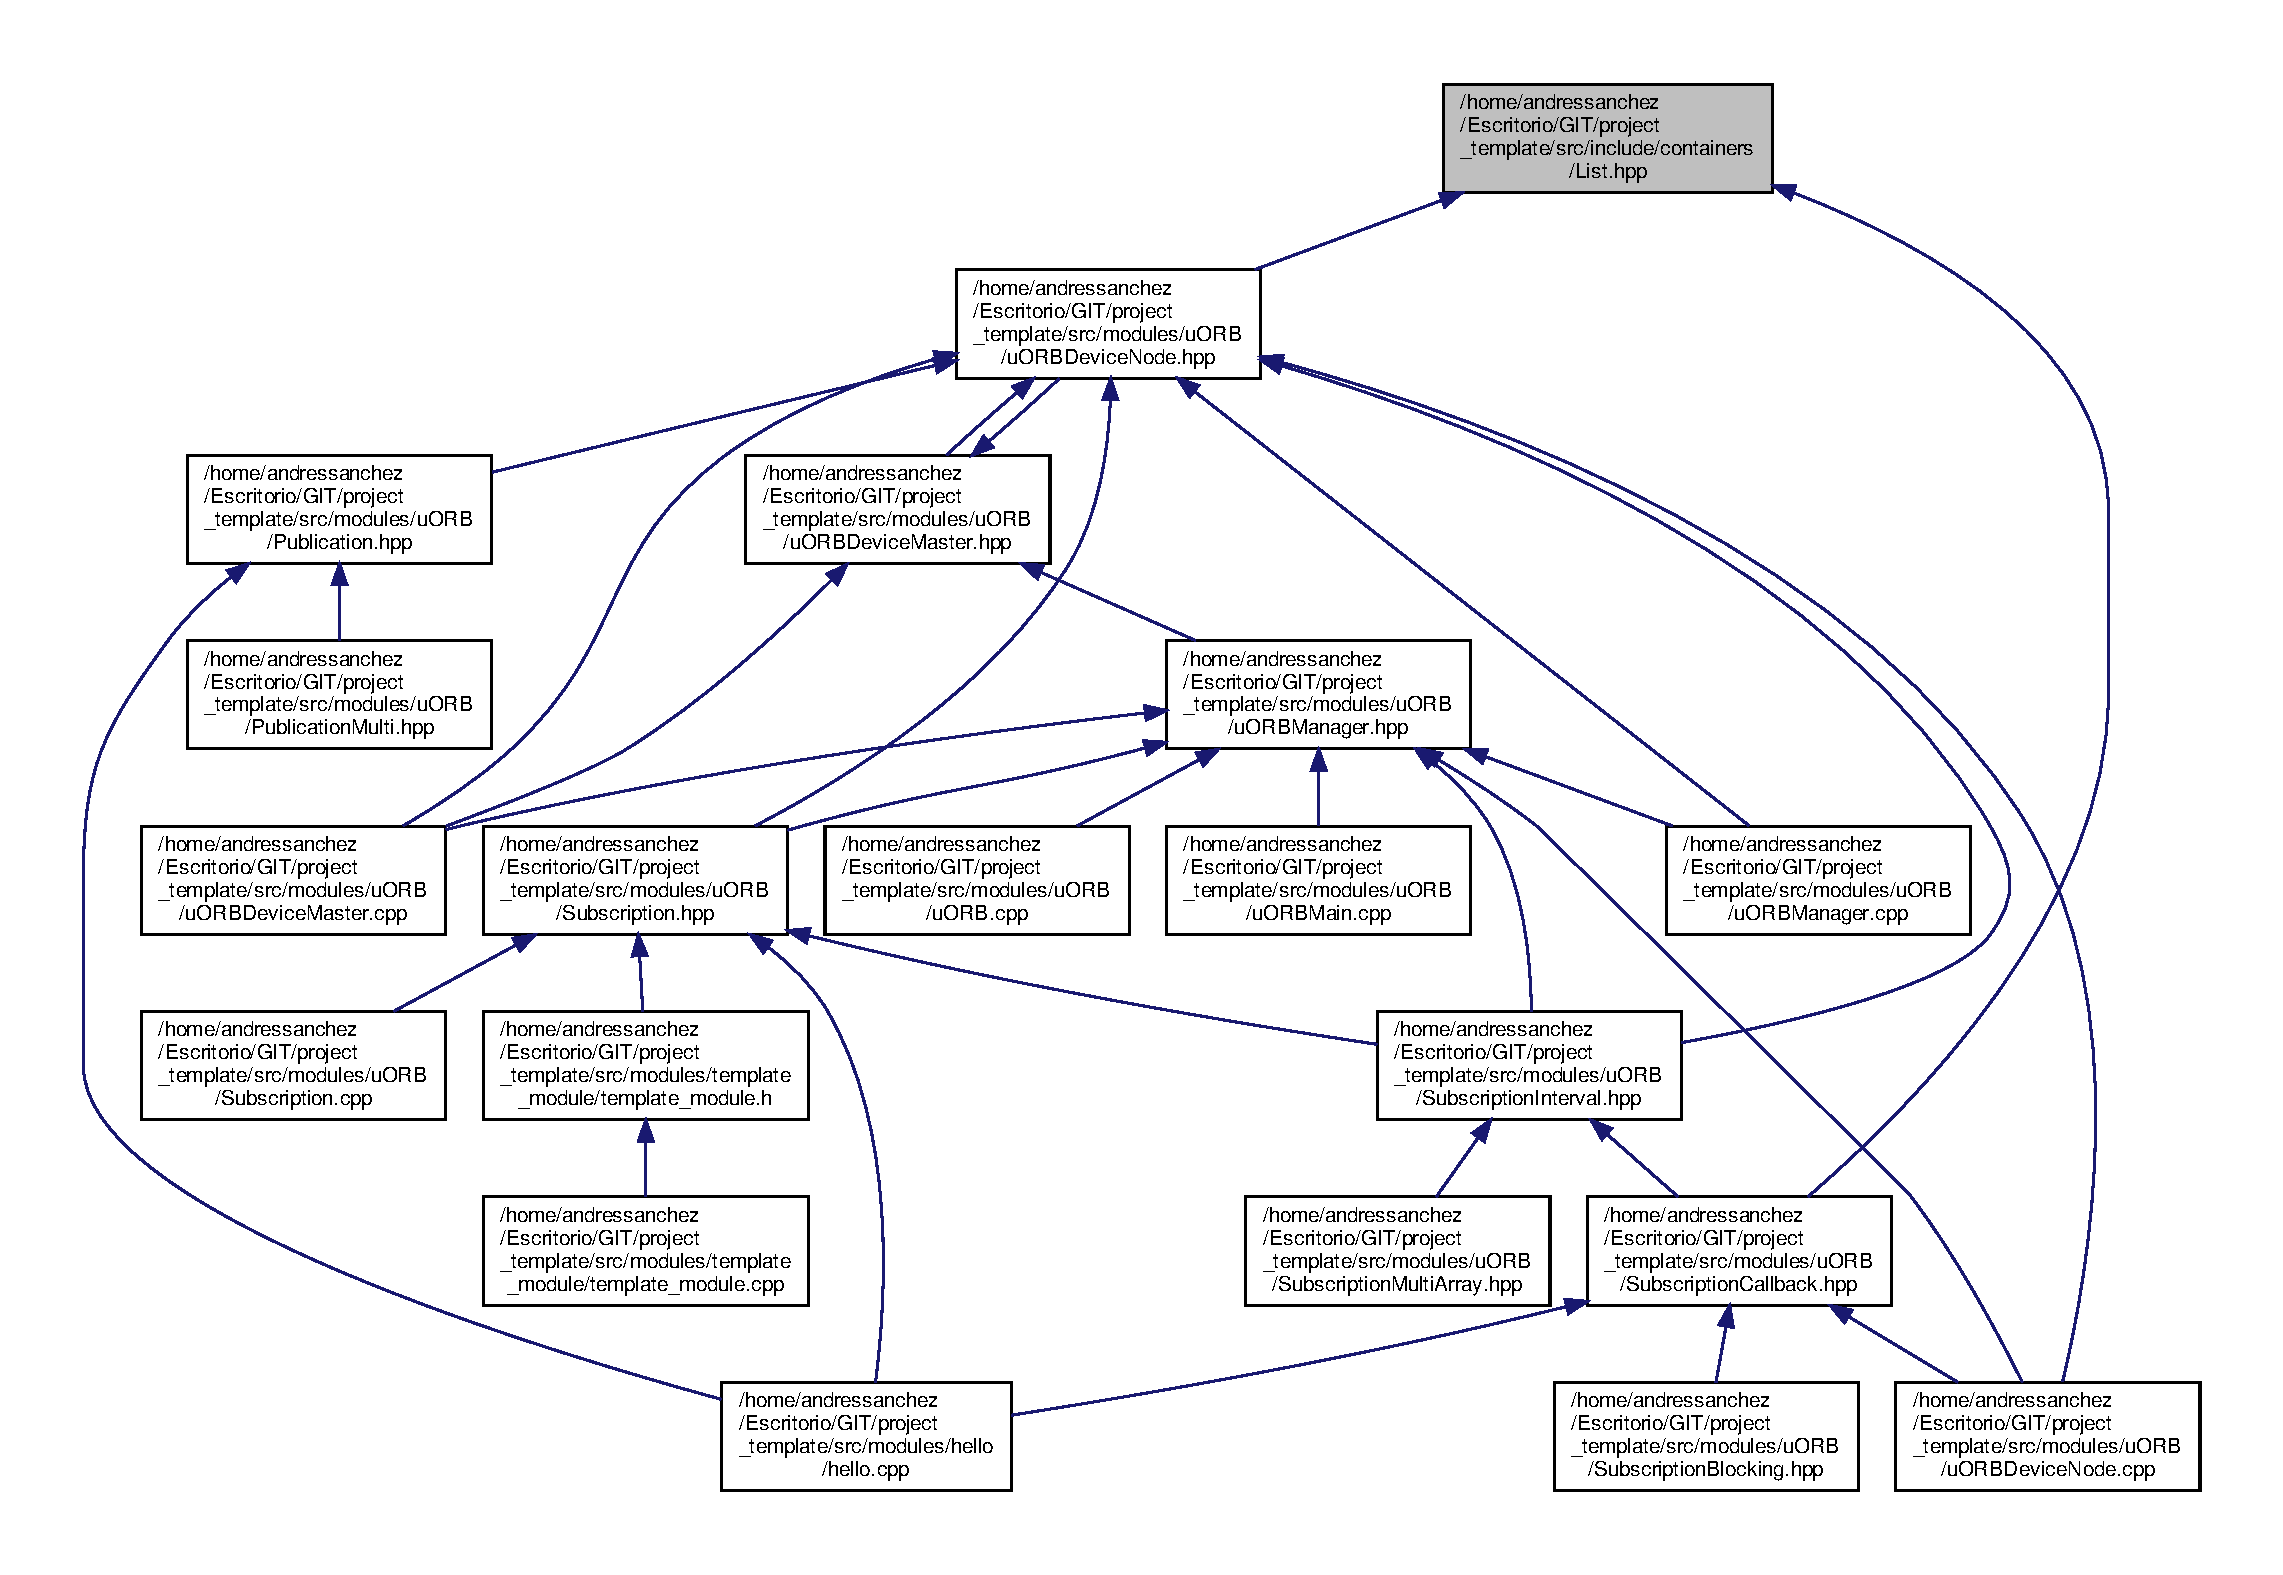
\includegraphics[width=350pt]{da/d00/List_8hpp__dep__incl}
\end{center}
\end{figure}
\subsection*{Classes}
\begin{DoxyCompactItemize}
\item 
class \hyperlink{classListNode}{List\+Node$<$ T $>$}
\item 
class \hyperlink{classList}{List$<$ T $>$}
\item 
struct \hyperlink{structList_1_1Iterator}{List$<$ T $>$\+::\+Iterator}
\end{DoxyCompactItemize}


\subsection{Detailed Description}
An intrusive linked list. 
\hypertarget{visibility_8h}{}\section{/home/andressanchez/\+Escritorio/\+G\+I\+T/project\+\_\+template/src/include/visibility.h File Reference}
\label{visibility_8h}\index{/home/andressanchez/\+Escritorio/\+G\+I\+T/project\+\_\+template/src/include/visibility.\+h@{/home/andressanchez/\+Escritorio/\+G\+I\+T/project\+\_\+template/src/include/visibility.\+h}}
{\ttfamily \#include $<$stdlib.\+h$>$}\newline
{\ttfamily \#include $<$time.\+h$>$}\newline
{\ttfamily \#include $<$pthread.\+h$>$}\newline
{\ttfamily \#include $<$unistd.\+h$>$}\newline
Include dependency graph for visibility.\+h\+:\nopagebreak
\begin{figure}[H]
\begin{center}
\leavevmode
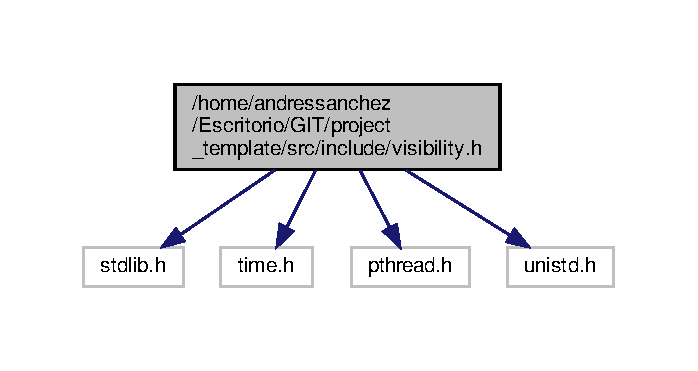
\includegraphics[width=335pt]{de/dda/visibility_8h__incl}
\end{center}
\end{figure}
\subsection*{Macros}
\begin{DoxyCompactItemize}
\item 
\mbox{\Hypertarget{visibility_8h_ad10ef148ba8327bd530fc6c32c1e181c}\label{visibility_8h_ad10ef148ba8327bd530fc6c32c1e181c}} 
\#define {\bfseries \+\_\+\+\_\+\+E\+X\+P\+O\+RT}~\+\_\+\+\_\+attribute\+\_\+\+\_\+ ((visibility (\char`\"{}default\char`\"{})))
\item 
\mbox{\Hypertarget{visibility_8h_aec1804eebbdabd0726d3116f4c48538f}\label{visibility_8h_aec1804eebbdabd0726d3116f4c48538f}} 
\#define {\bfseries \+\_\+\+\_\+\+P\+R\+I\+V\+A\+TE}~\+\_\+\+\_\+attribute\+\_\+\+\_\+ ((visibility (\char`\"{}hidden\char`\"{})))
\item 
\mbox{\Hypertarget{visibility_8h_a568e6bde99652b7fd271ad206cfe38f5}\label{visibility_8h_a568e6bde99652b7fd271ad206cfe38f5}} 
\#define {\bfseries \+\_\+\+\_\+\+B\+E\+G\+I\+N\+\_\+\+D\+E\+C\+LS}
\item 
\mbox{\Hypertarget{visibility_8h_a115472f6d0d1035f1885658ce0821537}\label{visibility_8h_a115472f6d0d1035f1885658ce0821537}} 
\#define {\bfseries \+\_\+\+\_\+\+E\+N\+D\+\_\+\+D\+E\+C\+LS}
\item 
\mbox{\Hypertarget{visibility_8h_a8aff4f29718e32ebdf0ebd54da4cdcc8}\label{visibility_8h_a8aff4f29718e32ebdf0ebd54da4cdcc8}} 
\#define {\bfseries system\+\_\+exit}~exit
\item 
\mbox{\Hypertarget{visibility_8h_a37e5b3149ac079fdc810b883acf34f78}\label{visibility_8h_a37e5b3149ac079fdc810b883acf34f78}} 
\#define {\bfseries system\+\_\+clock\+\_\+gettime}~clock\+\_\+gettime
\item 
\mbox{\Hypertarget{visibility_8h_a6b8f87ca70952144022b8f3871d1e52c}\label{visibility_8h_a6b8f87ca70952144022b8f3871d1e52c}} 
\#define {\bfseries system\+\_\+clock\+\_\+settime}~clock\+\_\+settime
\item 
\mbox{\Hypertarget{visibility_8h_a69c6df7eddd5b4c69515de90386d0ec9}\label{visibility_8h_a69c6df7eddd5b4c69515de90386d0ec9}} 
\#define {\bfseries system\+\_\+pthread\+\_\+cond\+\_\+timedwait}~pthread\+\_\+cond\+\_\+timedwait
\item 
\mbox{\Hypertarget{visibility_8h_ac91f1dfa3a3637967a53e38c9ee6f240}\label{visibility_8h_ac91f1dfa3a3637967a53e38c9ee6f240}} 
\#define {\bfseries system\+\_\+usleep}~usleep
\item 
\mbox{\Hypertarget{visibility_8h_af1e4397aa3029fbee85c47d135f3a4cb}\label{visibility_8h_af1e4397aa3029fbee85c47d135f3a4cb}} 
\#define {\bfseries system\+\_\+sleep}~sleep
\end{DoxyCompactItemize}


\subsection{Detailed Description}
Definitions controlling symbol naming and visibility.

This file is normally included automatically by the build system. 
\hypertarget{CDev_8cpp}{}\section{/home/andressanchez/\+Escritorio/\+G\+I\+T/project\+\_\+template/src/lib/cdev/\+C\+Dev.cpp File Reference}
\label{CDev_8cpp}\index{/home/andressanchez/\+Escritorio/\+G\+I\+T/project\+\_\+template/src/lib/cdev/\+C\+Dev.\+cpp@{/home/andressanchez/\+Escritorio/\+G\+I\+T/project\+\_\+template/src/lib/cdev/\+C\+Dev.\+cpp}}
{\ttfamily \#include \char`\"{}C\+Dev.\+hpp\char`\"{}}\newline
{\ttfamily \#include $<$nuttx/semaphore.\+h$>$}\newline
{\ttfamily \#include $<$nuttx/irq.\+h$>$}\newline
{\ttfamily \#include $<$nuttx/config.\+h$>$}\newline
{\ttfamily \#include $<$stdio.\+h$>$}\newline
{\ttfamily \#include $<$arch/irq.\+h$>$}\newline
{\ttfamily \#include $<$cstring$>$}\newline
Include dependency graph for C\+Dev.\+cpp\+:\nopagebreak
\begin{figure}[H]
\begin{center}
\leavevmode
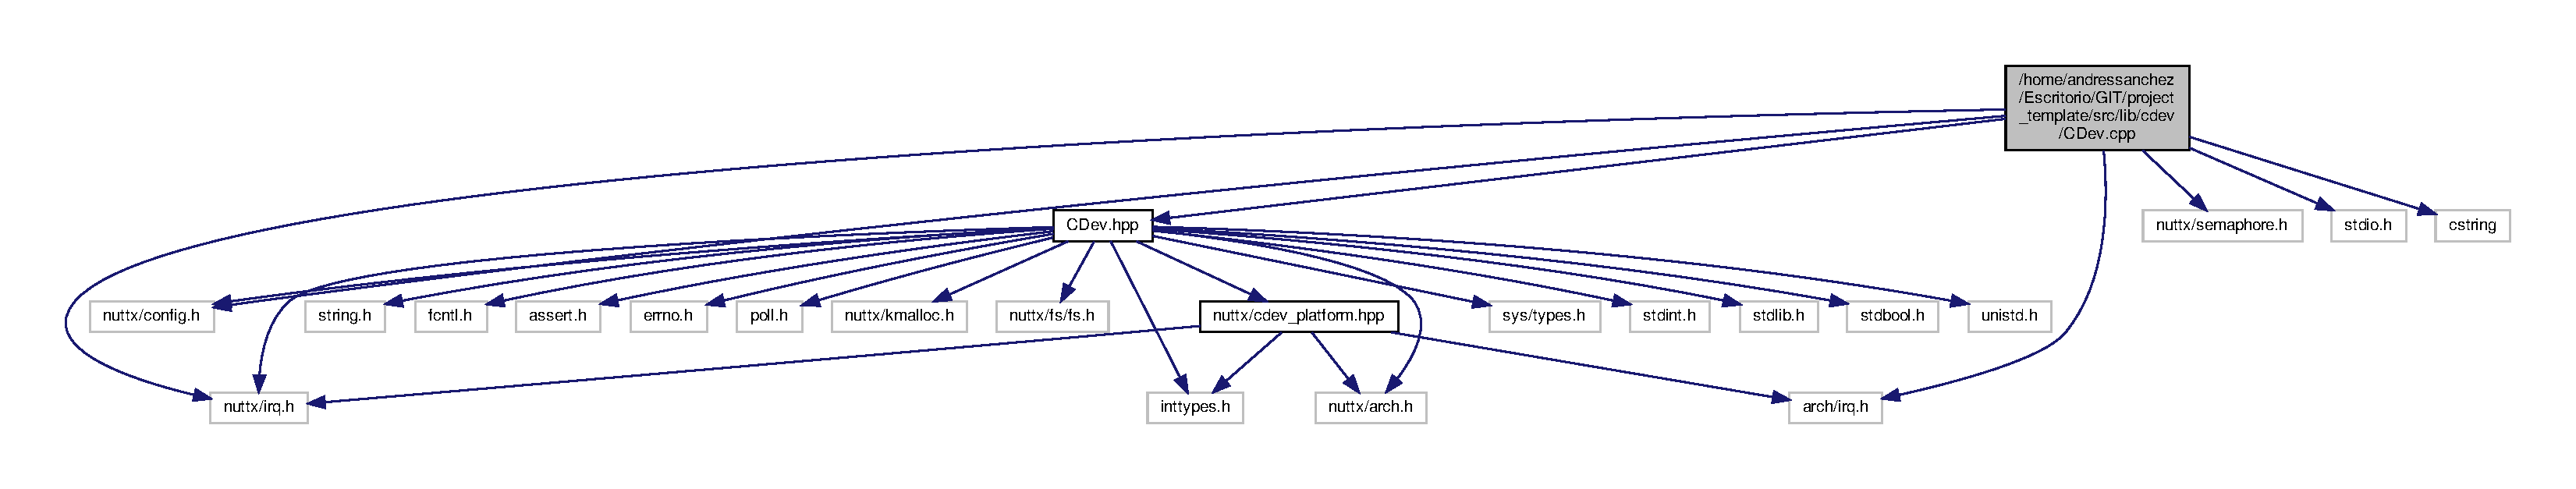
\includegraphics[width=350pt]{da/d54/CDev_8cpp__incl}
\end{center}
\end{figure}


\subsection{Detailed Description}
Character device base class. 
\hypertarget{CDev_8hpp}{}\section{/home/andressanchez/\+Escritorio/\+G\+I\+T/project\+\_\+template/src/lib/cdev/\+C\+Dev.hpp File Reference}
\label{CDev_8hpp}\index{/home/andressanchez/\+Escritorio/\+G\+I\+T/project\+\_\+template/src/lib/cdev/\+C\+Dev.\+hpp@{/home/andressanchez/\+Escritorio/\+G\+I\+T/project\+\_\+template/src/lib/cdev/\+C\+Dev.\+hpp}}
{\ttfamily \#include $<$nuttx/config.\+h$>$}\newline
{\ttfamily \#include $<$nuttx/kmalloc.\+h$>$}\newline
{\ttfamily \#include $<$nuttx/fs/fs.\+h$>$}\newline
{\ttfamily \#include $<$nuttx/arch.\+h$>$}\newline
{\ttfamily \#include $<$nuttx/irq.\+h$>$}\newline
{\ttfamily \#include $<$sys/types.\+h$>$}\newline
{\ttfamily \#include $<$inttypes.\+h$>$}\newline
{\ttfamily \#include $<$stdint.\+h$>$}\newline
{\ttfamily \#include $<$stdlib.\+h$>$}\newline
{\ttfamily \#include $<$stdbool.\+h$>$}\newline
{\ttfamily \#include $<$unistd.\+h$>$}\newline
{\ttfamily \#include $<$string.\+h$>$}\newline
{\ttfamily \#include $<$fcntl.\+h$>$}\newline
{\ttfamily \#include $<$assert.\+h$>$}\newline
{\ttfamily \#include $<$errno.\+h$>$}\newline
{\ttfamily \#include $<$poll.\+h$>$}\newline
{\ttfamily \#include \char`\"{}nuttx/cdev\+\_\+platform.\+hpp\char`\"{}}\newline
Include dependency graph for C\+Dev.\+hpp\+:\nopagebreak
\begin{figure}[H]
\begin{center}
\leavevmode
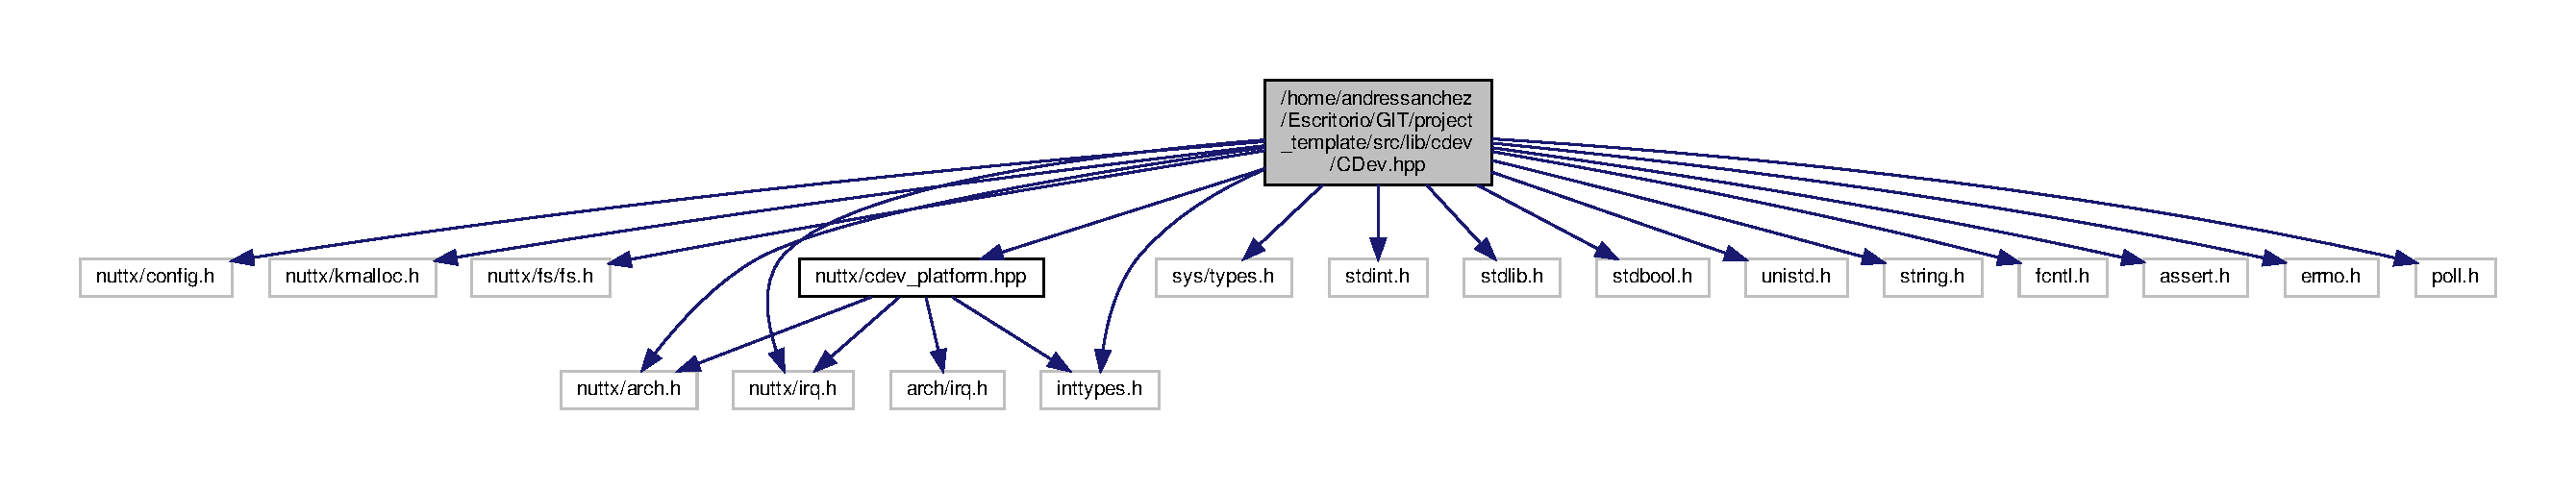
\includegraphics[width=350pt]{d3/d61/CDev_8hpp__incl}
\end{center}
\end{figure}
This graph shows which files directly or indirectly include this file\+:\nopagebreak
\begin{figure}[H]
\begin{center}
\leavevmode
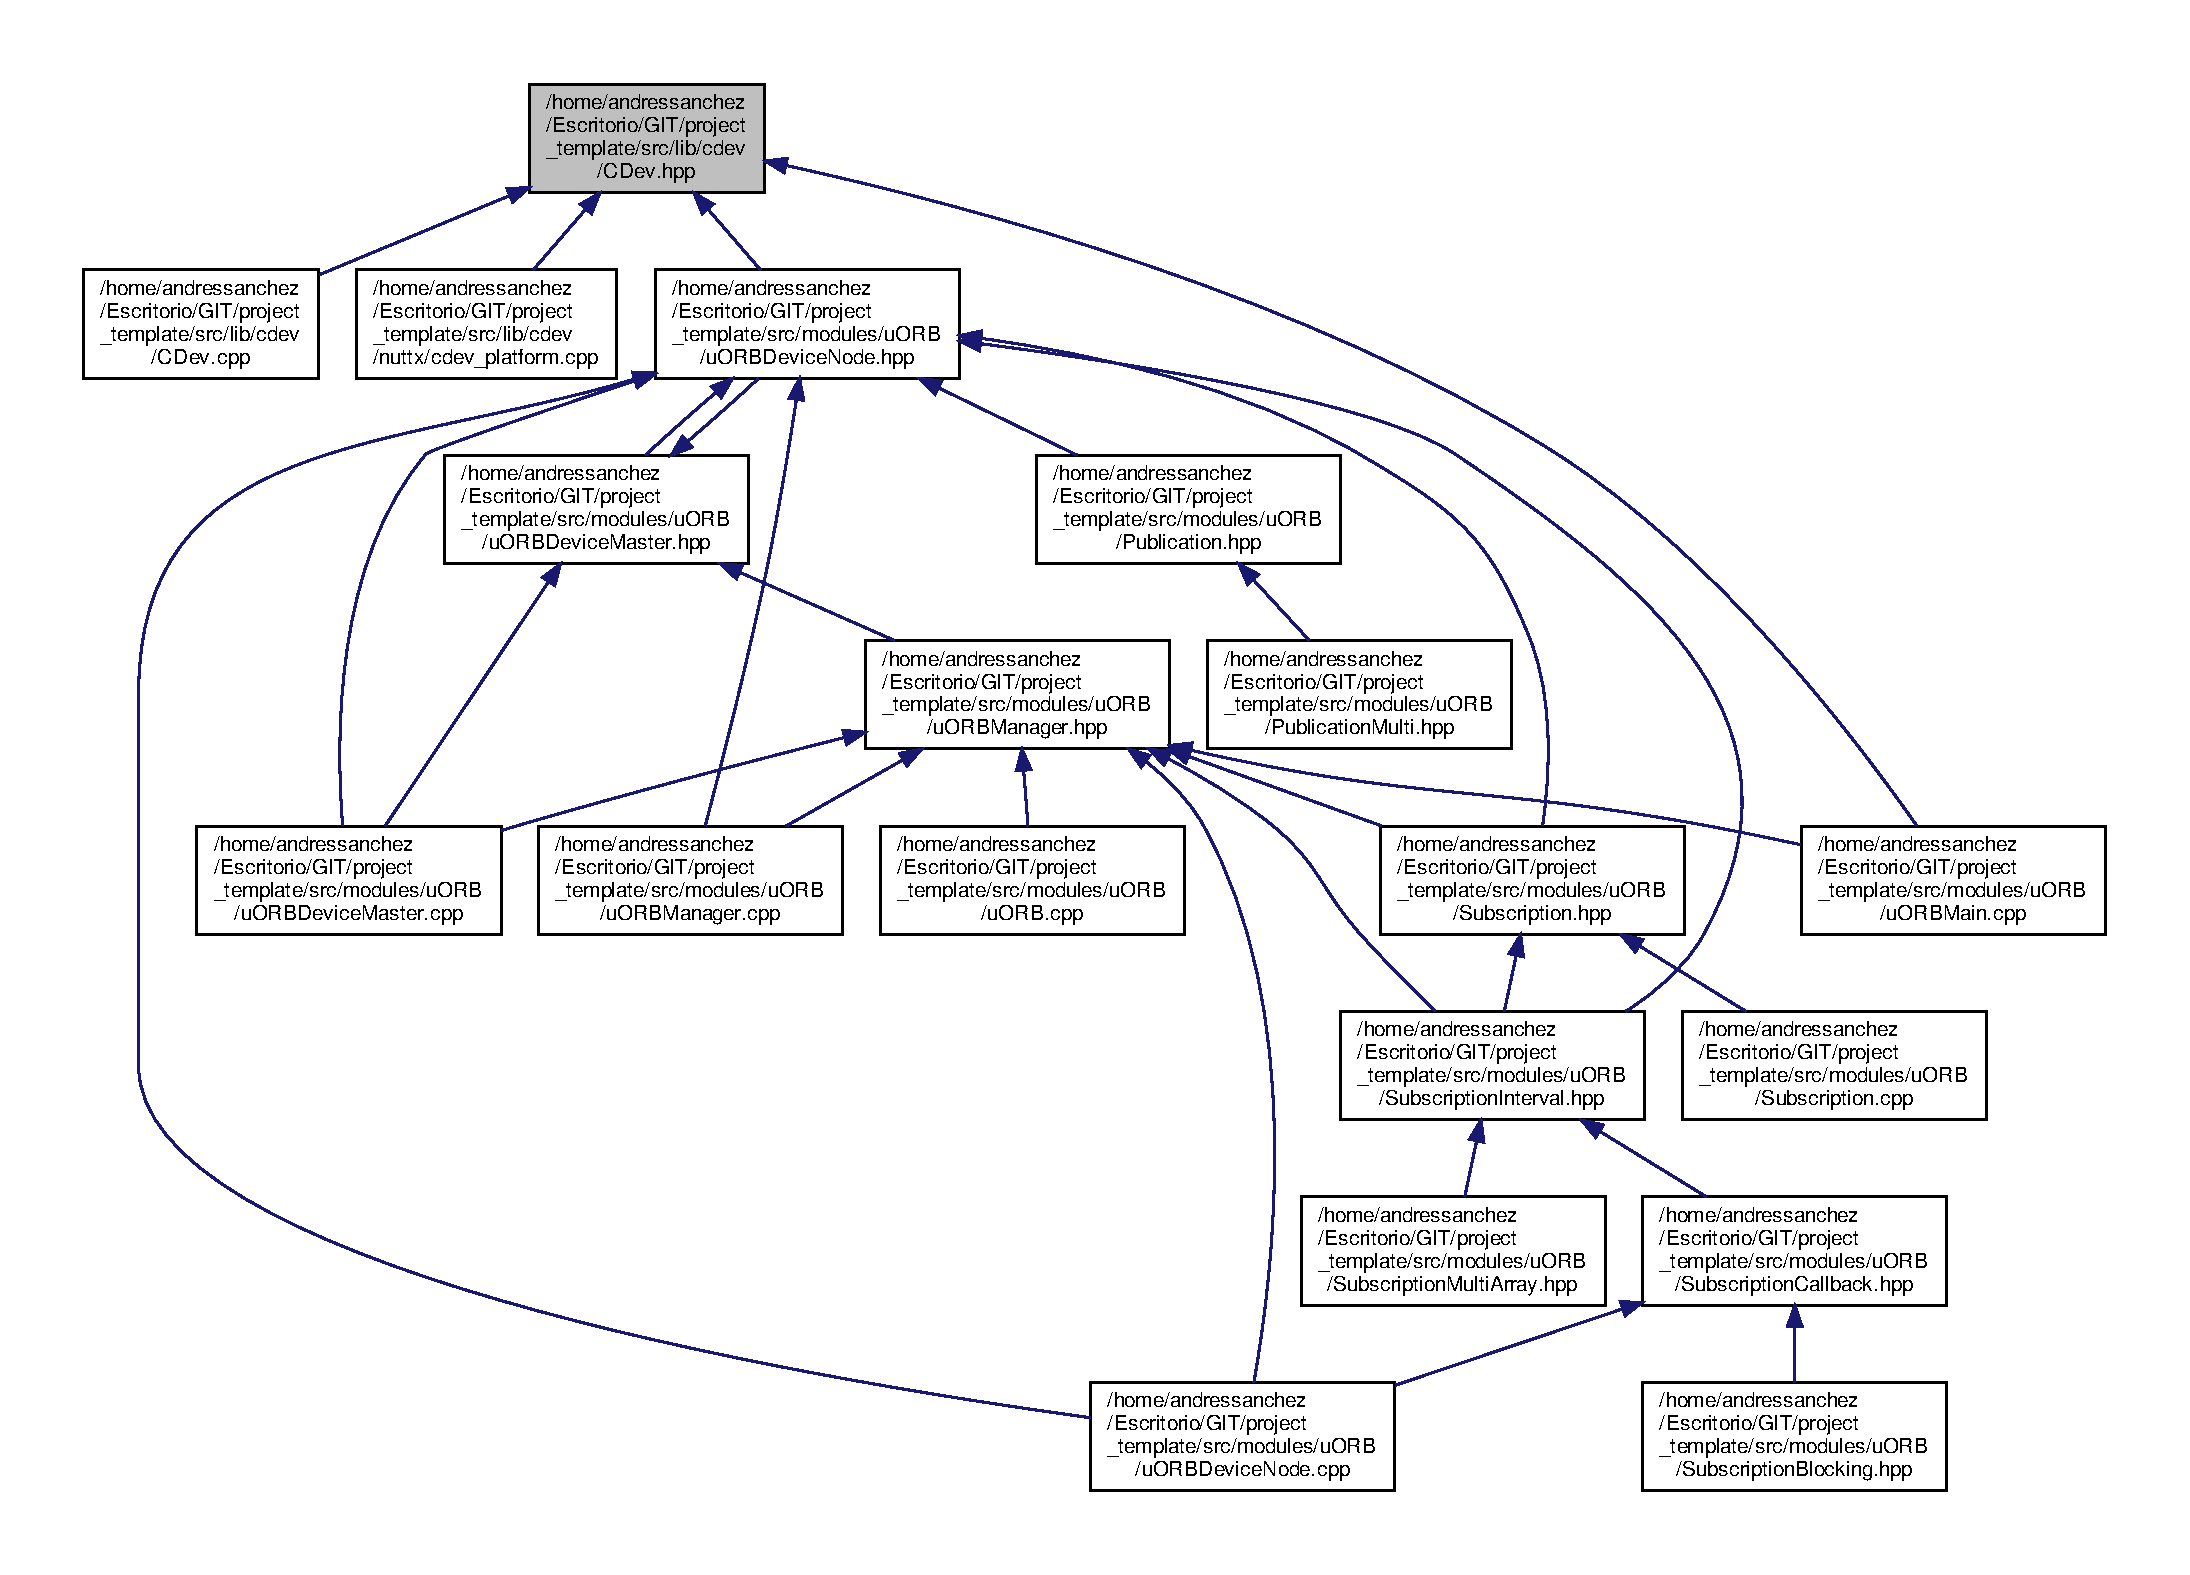
\includegraphics[width=350pt]{d1/d36/CDev_8hpp__dep__incl}
\end{center}
\end{figure}
\subsection*{Classes}
\begin{DoxyCompactItemize}
\item 
class \hyperlink{classcdev_1_1CDev}{cdev\+::\+C\+Dev}
\end{DoxyCompactItemize}


\subsection{Detailed Description}
Definitions for the generic base classes in the device framework. 
\hypertarget{cdev__platform_8cpp}{}\section{/home/andressanchez/\+Escritorio/\+G\+I\+T/project\+\_\+template/src/lib/cdev/nuttx/cdev\+\_\+platform.cpp File Reference}
\label{cdev__platform_8cpp}\index{/home/andressanchez/\+Escritorio/\+G\+I\+T/project\+\_\+template/src/lib/cdev/nuttx/cdev\+\_\+platform.\+cpp@{/home/andressanchez/\+Escritorio/\+G\+I\+T/project\+\_\+template/src/lib/cdev/nuttx/cdev\+\_\+platform.\+cpp}}
{\ttfamily \#include \char`\"{}cdev\+\_\+platform.\+hpp\char`\"{}}\newline
{\ttfamily \#include \char`\"{}../\+C\+Dev.\+hpp\char`\"{}}\newline
{\ttfamily \#include $<$sys/ioctl.\+h$>$}\newline
Include dependency graph for cdev\+\_\+platform.\+cpp\+:\nopagebreak
\begin{figure}[H]
\begin{center}
\leavevmode
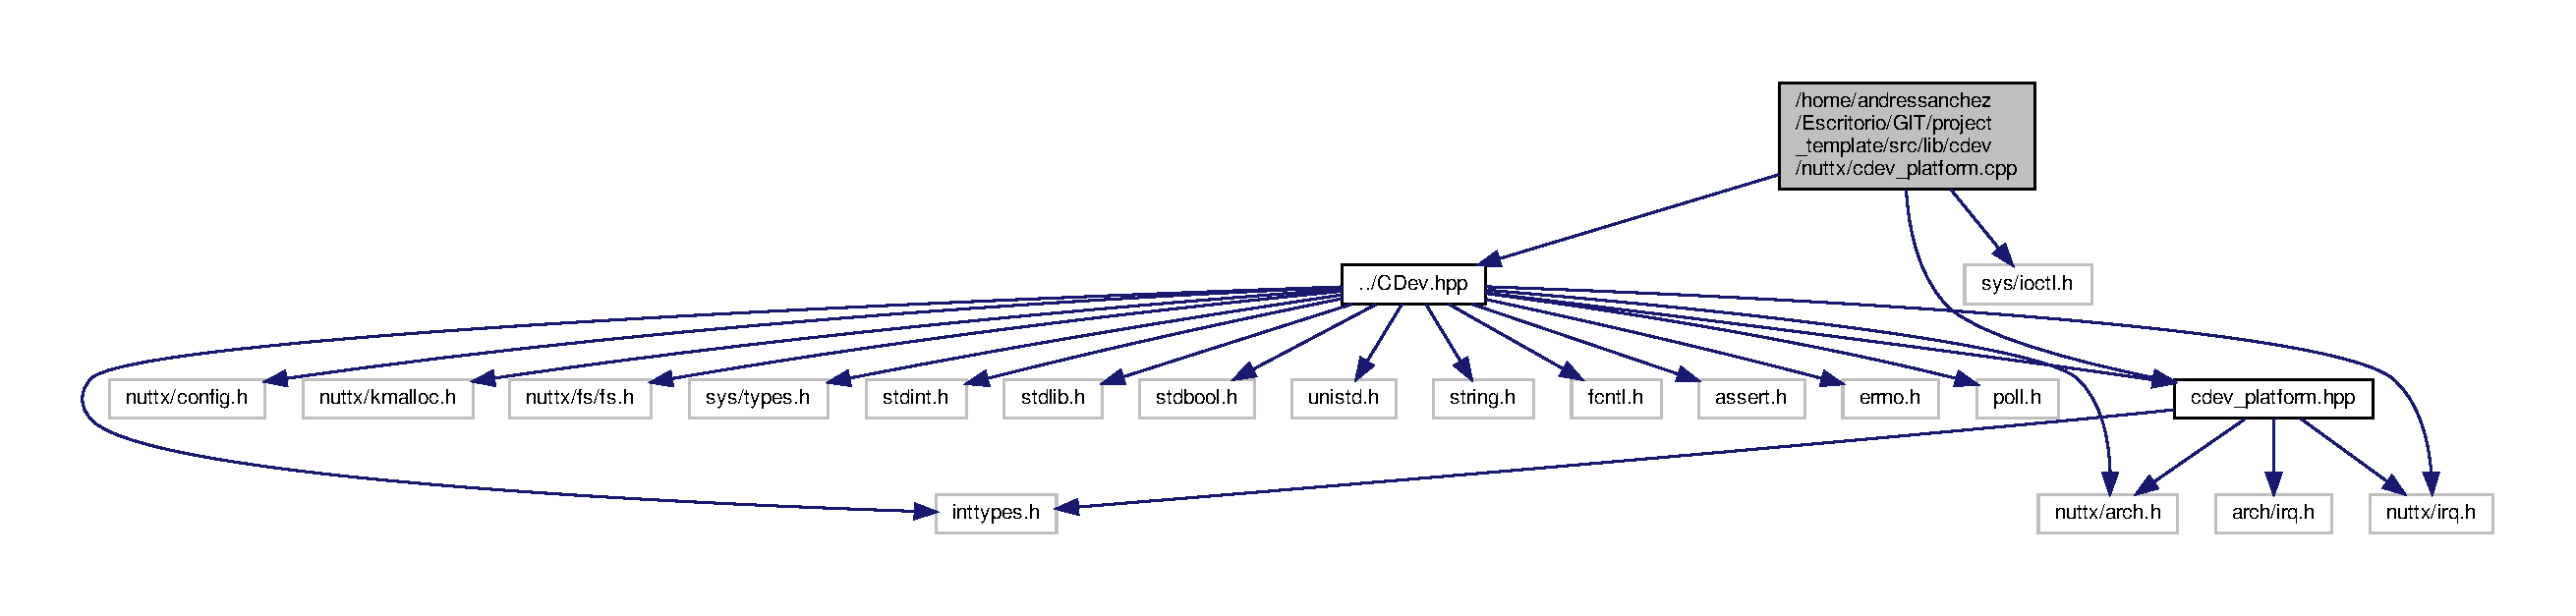
\includegraphics[width=350pt]{d1/d94/cdev__platform_8cpp__incl}
\end{center}
\end{figure}
\subsection*{Classes}
\begin{DoxyCompactItemize}
\item 
struct \hyperlink{structcdev_1_1cdev}{cdev\+::cdev}
\end{DoxyCompactItemize}


\subsection{Detailed Description}
NuttX Character device functions 
\hypertarget{version_8h}{}\section{/home/andressanchez/\+Escritorio/\+G\+I\+T/project\+\_\+template/src/lib/version/version.h File Reference}
\label{version_8h}\index{/home/andressanchez/\+Escritorio/\+G\+I\+T/project\+\_\+template/src/lib/version/version.\+h@{/home/andressanchez/\+Escritorio/\+G\+I\+T/project\+\_\+template/src/lib/version/version.\+h}}
{\ttfamily \#include $<$stdint.\+h$>$}\newline
Include dependency graph for version.\+h\+:
\nopagebreak
\begin{figure}[H]
\begin{center}
\leavevmode
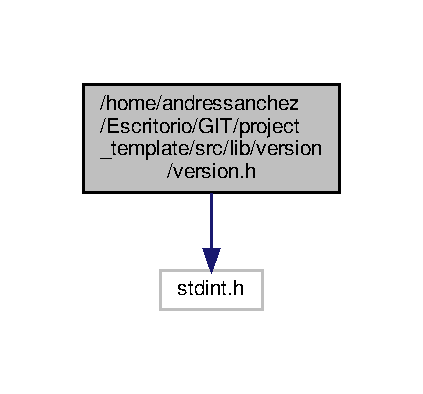
\includegraphics[width=203pt]{d8/d4a/version_8h__incl}
\end{center}
\end{figure}
This graph shows which files directly or indirectly include this file\+:
\nopagebreak
\begin{figure}[H]
\begin{center}
\leavevmode
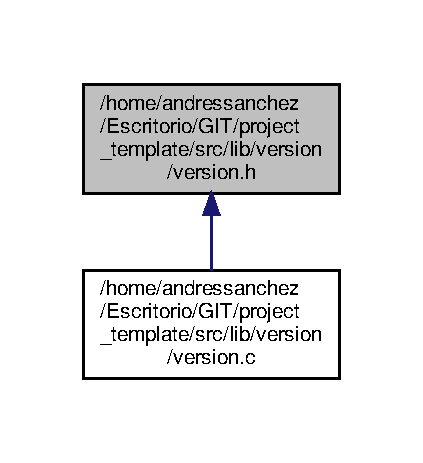
\includegraphics[width=203pt]{d2/deb/version_8h__dep__incl}
\end{center}
\end{figure}
\subsection*{Functions}
\begin{DoxyCompactItemize}
\item 
const char $\ast$ \hyperlink{version_8h_a20fc7c45a2af1951f1bda30a018034cf}{build\+\_\+uri} (void)
\item 
\+\_\+\+\_\+\+E\+X\+P\+O\+RT uint32\+\_\+t \hyperlink{version_8h_ae4d7c8bdf6528ebc410f1aced342f68b}{version\+\_\+tag\+\_\+to\+\_\+number} (const char $\ast$tag)
\item 
\+\_\+\+\_\+\+E\+X\+P\+O\+RT uint32\+\_\+t \hyperlink{version_8h_ade386147dba3b37795fc7f2ec688dd7e}{firmware\+\_\+version} (void)
\item 
\+\_\+\+\_\+\+E\+X\+P\+O\+RT uint32\+\_\+t \hyperlink{version_8h_ab74c0c1be88c621c4649792f2cae5343}{version\+\_\+tag\+\_\+to\+\_\+vendor\+\_\+version\+\_\+number} (const char $\ast$tag)
\item 
\+\_\+\+\_\+\+E\+X\+P\+O\+RT uint32\+\_\+t \hyperlink{version_8h_ae9561a342bd30d0b8e1fdf4393c7e470}{firmware\+\_\+vendor\+\_\+version} (void)
\item 
\+\_\+\+\_\+\+E\+X\+P\+O\+RT uint32\+\_\+t \hyperlink{version_8h_a722e4ea5c20929058c3629578feadaf1}{board\+\_\+version} (void)
\item 
\+\_\+\+\_\+\+E\+X\+P\+O\+RT uint32\+\_\+t \hyperlink{version_8h_a3602739b8e0d5879300a905785c8f371}{os\+\_\+version} (void)
\item 
\+\_\+\+\_\+\+E\+X\+P\+O\+RT const char $\ast$ \hyperlink{version_8h_a5839c1b79b14c6d5c08b1ff84500a971}{os\+\_\+version\+\_\+string} (void)
\item 
\+\_\+\+\_\+\+E\+X\+P\+O\+RT const char $\ast$ \hyperlink{version_8h_a575f337f7a850787f0271320d7859084}{os\+\_\+name} (void)
\item 
\+\_\+\+\_\+\+E\+X\+P\+O\+RT const char $\ast$ \hyperlink{version_8h_a10feca2b0b3de1a3a697cc7bcb90321e}{toolchain\+\_\+name} (void)
\item 
\+\_\+\+\_\+\+E\+X\+P\+O\+RT const char $\ast$ \hyperlink{version_8h_a6df22ceb4e1510ada6b5d742d411b9f9}{toolchain\+\_\+version} (void)
\item 
\+\_\+\+\_\+\+E\+X\+P\+O\+RT const char $\ast$ \hyperlink{version_8h_adb684265d41de587b8ce7eca29392be4}{firmware\+\_\+version\+\_\+string} (void)
\item 
\+\_\+\+\_\+\+E\+X\+P\+O\+RT const char $\ast$ \hyperlink{version_8h_a2705ca759e88988458f05d7d77fc4d87}{firmware\+\_\+git\+\_\+branch} (void)
\item 
\+\_\+\+\_\+\+E\+X\+P\+O\+RT uint64\+\_\+t \hyperlink{version_8h_a1600fb2282c2940e2dffa65585589702}{firmware\+\_\+version\+\_\+binary} (void)
\item 
\+\_\+\+\_\+\+E\+X\+P\+O\+RT const char $\ast$ \hyperlink{version_8h_a740c8b88768645ab5d0754210ebe678c}{ecl\+\_\+lib\+\_\+version\+\_\+string} (void)
\item 
\+\_\+\+\_\+\+E\+X\+P\+O\+RT uint64\+\_\+t \hyperlink{version_8h_a56604d1940f59bed9a41ac57b8f92629}{mavlink\+\_\+lib\+\_\+version\+\_\+binary} (void)
\item 
\+\_\+\+\_\+\+E\+X\+P\+O\+RT uint64\+\_\+t \hyperlink{version_8h_a8534281b0ffc293781e6cd4c04e30e82}{os\+\_\+version\+\_\+binary} (void)
\end{DoxyCompactItemize}


\subsection{Detailed Description}
Tools for system version detection.

\begin{DoxyAuthor}{Author}
Anton Babushkin \href{mailto:anton.babushkin@me.com}{\tt anton.\+babushkin@me.\+com} 

Beat Küng \href{mailto:beat-kueng@gmx.net}{\tt beat-\/kueng@gmx.\+net} 
\end{DoxyAuthor}


\subsection{Function Documentation}
\mbox{\Hypertarget{version_8h_a722e4ea5c20929058c3629578feadaf1}\label{version_8h_a722e4ea5c20929058c3629578feadaf1}} 
\index{version.\+h@{version.\+h}!board\+\_\+version@{board\+\_\+version}}
\index{board\+\_\+version@{board\+\_\+version}!version.\+h@{version.\+h}}
\subsubsection{\texorpdfstring{board\+\_\+version()}{board\_version()}}
{\footnotesize\ttfamily \+\_\+\+\_\+\+E\+X\+P\+O\+RT uint32\+\_\+t board\+\_\+version (\begin{DoxyParamCaption}\item[{void}]{ }\end{DoxyParamCaption})}

get the board version (last 8 bytes should be silicon ID, if any) 

Definition at line 248 of file version.\+c.


\begin{DoxyCode}
249 \{
250 \textcolor{preprocessor}{#if defined(\_\_NUTTX)}
251     \textcolor{keywordflow}{return} CONFIG\_CDCACM\_PRODUCTID;
252 \textcolor{preprocessor}{#else}
253     \textcolor{keywordflow}{return} 1;
254 \textcolor{preprocessor}{#endif}
255 \}
\end{DoxyCode}
\mbox{\Hypertarget{version_8h_a20fc7c45a2af1951f1bda30a018034cf}\label{version_8h_a20fc7c45a2af1951f1bda30a018034cf}} 
\index{version.\+h@{version.\+h}!build\+\_\+uri@{build\+\_\+uri}}
\index{build\+\_\+uri@{build\+\_\+uri}!version.\+h@{version.\+h}}
\subsubsection{\texorpdfstring{build\+\_\+uri()}{build\_uri()}}
{\footnotesize\ttfamily const char$\ast$ build\+\_\+uri (\begin{DoxyParamCaption}\item[{void}]{ }\end{DoxyParamCaption})}

get the build U\+RI (used for crash logging) 

Definition at line 59 of file version.\+c.


\begin{DoxyCode}
60 \{
61     \textcolor{keywordflow}{return} STRINGIFY(BUILD\_URI);
62 \}
\end{DoxyCode}
\mbox{\Hypertarget{version_8h_a740c8b88768645ab5d0754210ebe678c}\label{version_8h_a740c8b88768645ab5d0754210ebe678c}} 
\index{version.\+h@{version.\+h}!ecl\+\_\+lib\+\_\+version\+\_\+string@{ecl\+\_\+lib\+\_\+version\+\_\+string}}
\index{ecl\+\_\+lib\+\_\+version\+\_\+string@{ecl\+\_\+lib\+\_\+version\+\_\+string}!version.\+h@{version.\+h}}
\subsubsection{\texorpdfstring{ecl\+\_\+lib\+\_\+version\+\_\+string()}{ecl\_lib\_version\_string()}}
{\footnotesize\ttfamily \+\_\+\+\_\+\+E\+X\+P\+O\+RT const char$\ast$ ecl\+\_\+lib\+\_\+version\+\_\+string (\begin{DoxyParamCaption}\item[{void}]{ }\end{DoxyParamCaption})}

E\+CL lib version as human readable string (git tag) 

Definition at line 346 of file version.\+c.


\begin{DoxyCode}
347 \{
348 \textcolor{preprocessor}{#ifdef ECL\_LIB\_GIT\_VERSION\_STRING}
349     \textcolor{keywordflow}{return} ECL\_LIB\_GIT\_VERSION\_STRING;
350 \textcolor{preprocessor}{#else}
351     \textcolor{keywordflow}{return} NULL;
352 \textcolor{preprocessor}{#endif}
353 \}
\end{DoxyCode}
\mbox{\Hypertarget{version_8h_a2705ca759e88988458f05d7d77fc4d87}\label{version_8h_a2705ca759e88988458f05d7d77fc4d87}} 
\index{version.\+h@{version.\+h}!firmware\+\_\+git\+\_\+branch@{firmware\+\_\+git\+\_\+branch}}
\index{firmware\+\_\+git\+\_\+branch@{firmware\+\_\+git\+\_\+branch}!version.\+h@{version.\+h}}
\subsubsection{\texorpdfstring{firmware\+\_\+git\+\_\+branch()}{firmware\_git\_branch()}}
{\footnotesize\ttfamily \+\_\+\+\_\+\+E\+X\+P\+O\+RT const char$\ast$ firmware\+\_\+git\+\_\+branch (\begin{DoxyParamCaption}\item[{void}]{ }\end{DoxyParamCaption})}

get the git branch name (can be empty, for example if H\+E\+AD points to a tag) 

Definition at line 243 of file version.\+c.


\begin{DoxyCode}
244 \{
245     \textcolor{keywordflow}{return} GIT\_BRANCH\_NAME;
246 \}
\end{DoxyCode}
\mbox{\Hypertarget{version_8h_ae9561a342bd30d0b8e1fdf4393c7e470}\label{version_8h_ae9561a342bd30d0b8e1fdf4393c7e470}} 
\index{version.\+h@{version.\+h}!firmware\+\_\+vendor\+\_\+version@{firmware\+\_\+vendor\+\_\+version}}
\index{firmware\+\_\+vendor\+\_\+version@{firmware\+\_\+vendor\+\_\+version}!version.\+h@{version.\+h}}
\subsubsection{\texorpdfstring{firmware\+\_\+vendor\+\_\+version()}{firmware\_vendor\_version()}}
{\footnotesize\ttfamily \+\_\+\+\_\+\+E\+X\+P\+O\+RT uint32\+\_\+t firmware\+\_\+vendor\+\_\+version (\begin{DoxyParamCaption}\item[{void}]{ }\end{DoxyParamCaption})}

get the P\+X4 Firmware vendor version \begin{DoxyReturn}{Returns}
version in the form 0x\+A\+A\+B\+B\+C\+C\+TT (AA\+: Major, BB\+: Minor, CC\+: Patch, TT Type 
\end{DoxyReturn}
\begin{DoxySeeAlso}{See also}
F\+I\+R\+M\+W\+A\+R\+E\+\_\+\+T\+Y\+PE) 
\end{DoxySeeAlso}


Definition at line 238 of file version.\+c.


\begin{DoxyCode}
239 \{
240     \textcolor{keywordflow}{return} \hyperlink{version_8h_ab74c0c1be88c621c4649792f2cae5343}{version\_tag\_to\_vendor\_version\_number}(GIT\_TAG\_STR);
241 \}
\end{DoxyCode}
\mbox{\Hypertarget{version_8h_ade386147dba3b37795fc7f2ec688dd7e}\label{version_8h_ade386147dba3b37795fc7f2ec688dd7e}} 
\index{version.\+h@{version.\+h}!firmware\+\_\+version@{firmware\+\_\+version}}
\index{firmware\+\_\+version@{firmware\+\_\+version}!version.\+h@{version.\+h}}
\subsubsection{\texorpdfstring{firmware\+\_\+version()}{firmware\_version()}}
{\footnotesize\ttfamily \+\_\+\+\_\+\+E\+X\+P\+O\+RT uint32\+\_\+t firmware\+\_\+version (\begin{DoxyParamCaption}\item[{void}]{ }\end{DoxyParamCaption})}

get the P\+X4 Firmware version \begin{DoxyReturn}{Returns}
version in the form 0x\+A\+A\+B\+B\+C\+C\+TT (AA\+: Major, BB\+: Minor, CC\+: Patch, TT Type 
\end{DoxyReturn}
\begin{DoxySeeAlso}{See also}
F\+I\+R\+M\+W\+A\+R\+E\+\_\+\+T\+Y\+PE) 
\end{DoxySeeAlso}


Definition at line 147 of file version.\+c.


\begin{DoxyCode}
148 \{
149     \textcolor{keywordflow}{return} \hyperlink{version_8h_ae4d7c8bdf6528ebc410f1aced342f68b}{version\_tag\_to\_number}(GIT\_TAG\_STR);
150 \}
\end{DoxyCode}
\mbox{\Hypertarget{version_8h_a1600fb2282c2940e2dffa65585589702}\label{version_8h_a1600fb2282c2940e2dffa65585589702}} 
\index{version.\+h@{version.\+h}!firmware\+\_\+version\+\_\+binary@{firmware\+\_\+version\+\_\+binary}}
\index{firmware\+\_\+version\+\_\+binary@{firmware\+\_\+version\+\_\+binary}!version.\+h@{version.\+h}}
\subsubsection{\texorpdfstring{firmware\+\_\+version\+\_\+binary()}{firmware\_version\_binary()}}
{\footnotesize\ttfamily \+\_\+\+\_\+\+E\+X\+P\+O\+RT uint64\+\_\+t firmware\+\_\+version\+\_\+binary (\begin{DoxyParamCaption}\item[{void}]{ }\end{DoxyParamCaption})}

Firmware version in binary form (first part of the git tag) 

Definition at line 341 of file version.\+c.


\begin{DoxyCode}
342 \{
343     \textcolor{keywordflow}{return} GIT\_VERSION\_BINARY;
344 \}
\end{DoxyCode}
\mbox{\Hypertarget{version_8h_adb684265d41de587b8ce7eca29392be4}\label{version_8h_adb684265d41de587b8ce7eca29392be4}} 
\index{version.\+h@{version.\+h}!firmware\+\_\+version\+\_\+string@{firmware\+\_\+version\+\_\+string}}
\index{firmware\+\_\+version\+\_\+string@{firmware\+\_\+version\+\_\+string}!version.\+h@{version.\+h}}
\subsubsection{\texorpdfstring{firmware\+\_\+version\+\_\+string()}{firmware\_version\_string()}}
{\footnotesize\ttfamily \+\_\+\+\_\+\+E\+X\+P\+O\+RT const char$\ast$ firmware\+\_\+version\+\_\+string (\begin{DoxyParamCaption}\item[{void}]{ }\end{DoxyParamCaption})}

Firmware version as human readable string (git tag) 

Definition at line 336 of file version.\+c.


\begin{DoxyCode}
337 \{
338     \textcolor{keywordflow}{return} GIT\_VERSION\_STR;
339 \}
\end{DoxyCode}
\mbox{\Hypertarget{version_8h_a56604d1940f59bed9a41ac57b8f92629}\label{version_8h_a56604d1940f59bed9a41ac57b8f92629}} 
\index{version.\+h@{version.\+h}!mavlink\+\_\+lib\+\_\+version\+\_\+binary@{mavlink\+\_\+lib\+\_\+version\+\_\+binary}}
\index{mavlink\+\_\+lib\+\_\+version\+\_\+binary@{mavlink\+\_\+lib\+\_\+version\+\_\+binary}!version.\+h@{version.\+h}}
\subsubsection{\texorpdfstring{mavlink\+\_\+lib\+\_\+version\+\_\+binary()}{mavlink\_lib\_version\_binary()}}
{\footnotesize\ttfamily \+\_\+\+\_\+\+E\+X\+P\+O\+RT uint64\+\_\+t mavlink\+\_\+lib\+\_\+version\+\_\+binary (\begin{DoxyParamCaption}\item[{void}]{ }\end{DoxyParamCaption})}

M\+A\+V\+Link lib version in binary form (first part of the git tag) \mbox{\Hypertarget{version_8h_a575f337f7a850787f0271320d7859084}\label{version_8h_a575f337f7a850787f0271320d7859084}} 
\index{version.\+h@{version.\+h}!os\+\_\+name@{os\+\_\+name}}
\index{os\+\_\+name@{os\+\_\+name}!version.\+h@{version.\+h}}
\subsubsection{\texorpdfstring{os\+\_\+name()}{os\_name()}}
{\footnotesize\ttfamily \+\_\+\+\_\+\+E\+X\+P\+O\+RT const char$\ast$ os\+\_\+name (\begin{DoxyParamCaption}\item[{void}]{ }\end{DoxyParamCaption})}

name of the operating system \begin{DoxyReturn}{Returns}
human readable string 
\end{DoxyReturn}


Definition at line 295 of file version.\+c.


\begin{DoxyCode}
296 \{
297 \textcolor{preprocessor}{#if defined(\_\_DARWIN)}
298     \textcolor{keywordflow}{return} \textcolor{stringliteral}{"Darwin"};
299 \textcolor{preprocessor}{#elif defined(\_\_LINUX)}
300     \textcolor{keywordflow}{return} \textcolor{stringliteral}{"Linux"};
301 \textcolor{preprocessor}{#elif defined(\_\_QURT)}
302     \textcolor{keywordflow}{return} \textcolor{stringliteral}{"QuRT"};
303 \textcolor{preprocessor}{#elif defined(\_\_NUTTX)}
304     \textcolor{keywordflow}{return} \textcolor{stringliteral}{"NuttX"};
305 \textcolor{preprocessor}{#elif defined(\_\_CYGWIN)}
306     \textcolor{keywordflow}{return} \textcolor{stringliteral}{"Cygwin"};
307 \textcolor{preprocessor}{#else}
308 \textcolor{preprocessor}{# error "os\_name not implemented for current OS"}
309 \textcolor{preprocessor}{#endif}
310 \}
\end{DoxyCode}
\mbox{\Hypertarget{version_8h_a3602739b8e0d5879300a905785c8f371}\label{version_8h_a3602739b8e0d5879300a905785c8f371}} 
\index{version.\+h@{version.\+h}!os\+\_\+version@{os\+\_\+version}}
\index{os\+\_\+version@{os\+\_\+version}!version.\+h@{version.\+h}}
\subsubsection{\texorpdfstring{os\+\_\+version()}{os\_version()}}
{\footnotesize\ttfamily \+\_\+\+\_\+\+E\+X\+P\+O\+RT uint32\+\_\+t os\+\_\+version (\begin{DoxyParamCaption}\item[{void}]{ }\end{DoxyParamCaption})}

operating system version \begin{DoxyReturn}{Returns}
version in the form 0x\+A\+A\+B\+B\+C\+C\+TT (AA\+: Major, BB\+: Minor, CC\+: Patch, TT Type 
\end{DoxyReturn}
\begin{DoxySeeAlso}{See also}
F\+I\+R\+M\+W\+A\+R\+E\+\_\+\+T\+Y\+PE) 
\end{DoxySeeAlso}


Definition at line 257 of file version.\+c.


\begin{DoxyCode}
258 \{
259 \textcolor{preprocessor}{#if defined(\_\_DARWIN) || defined(\_\_CYGWIN) || defined(\_\_QURT)}
260     \textcolor{keywordflow}{return} 0; \textcolor{comment}{//TODO: implement version for Darwin, Cygwin, QuRT}
261 \textcolor{preprocessor}{#elif defined(\_\_LINUX)}
262     \textcolor{keyword}{struct }utsname name;
263 
264     \textcolor{keywordflow}{if} (uname(&name) == 0) \{
265         \textcolor{keywordtype}{char} *c = name.release;
266 
267         \textcolor{comment}{// cut the part after the first '-'}
268         \textcolor{keywordflow}{while} (*c && *c != \textcolor{charliteral}{'-'}) \{
269             ++c;
270         \}
271 
272         *c = 0;
273         \textcolor{keywordflow}{return} \hyperlink{version_8h_ae4d7c8bdf6528ebc410f1aced342f68b}{version\_tag\_to\_number}(name.release);
274 
275     \} \textcolor{keywordflow}{else} \{
276         \textcolor{keywordflow}{return} 0;
277     \}
278 
279 \textcolor{preprocessor}{#elif defined(\_\_NUTTX)}
280     \textcolor{keywordflow}{return} \hyperlink{version_8h_ae4d7c8bdf6528ebc410f1aced342f68b}{version\_tag\_to\_number}(NUTTX\_GIT\_TAG\_STR);
281 \textcolor{preprocessor}{#else}
282 \textcolor{preprocessor}{# error "os\_version not implemented for current OS"}
283 \textcolor{preprocessor}{#endif}
284 \}
\end{DoxyCode}
\mbox{\Hypertarget{version_8h_a8534281b0ffc293781e6cd4c04e30e82}\label{version_8h_a8534281b0ffc293781e6cd4c04e30e82}} 
\index{version.\+h@{version.\+h}!os\+\_\+version\+\_\+binary@{os\+\_\+version\+\_\+binary}}
\index{os\+\_\+version\+\_\+binary@{os\+\_\+version\+\_\+binary}!version.\+h@{version.\+h}}
\subsubsection{\texorpdfstring{os\+\_\+version\+\_\+binary()}{os\_version\_binary()}}
{\footnotesize\ttfamily \+\_\+\+\_\+\+E\+X\+P\+O\+RT uint64\+\_\+t os\+\_\+version\+\_\+binary (\begin{DoxyParamCaption}\item[{void}]{ }\end{DoxyParamCaption})}

Operating system version in binary form (first part of the git tag) \begin{DoxyReturn}{Returns}
this is not available on all O\+Ses and can return 0 
\end{DoxyReturn}


Definition at line 362 of file version.\+c.


\begin{DoxyCode}
363 \{
364 \textcolor{preprocessor}{#ifdef NUTTX\_GIT\_VERSION\_BINARY}
365     \textcolor{keywordflow}{return} NUTTX\_GIT\_VERSION\_BINARY;
366 \textcolor{preprocessor}{#else}
367     \textcolor{keywordflow}{return} 0;
368 \textcolor{preprocessor}{#endif}
369 \}
\end{DoxyCode}
\mbox{\Hypertarget{version_8h_a5839c1b79b14c6d5c08b1ff84500a971}\label{version_8h_a5839c1b79b14c6d5c08b1ff84500a971}} 
\index{version.\+h@{version.\+h}!os\+\_\+version\+\_\+string@{os\+\_\+version\+\_\+string}}
\index{os\+\_\+version\+\_\+string@{os\+\_\+version\+\_\+string}!version.\+h@{version.\+h}}
\subsubsection{\texorpdfstring{os\+\_\+version\+\_\+string()}{os\_version\_string()}}
{\footnotesize\ttfamily \+\_\+\+\_\+\+E\+X\+P\+O\+RT const char$\ast$ os\+\_\+version\+\_\+string (\begin{DoxyParamCaption}\item[{void}]{ }\end{DoxyParamCaption})}

Operating system version as human readable string (git tag) \begin{DoxyReturn}{Returns}
string or N\+U\+LL if not defined 
\end{DoxyReturn}


Definition at line 286 of file version.\+c.


\begin{DoxyCode}
287 \{
288 \textcolor{preprocessor}{#if defined(\_\_NUTTX)}
289     \textcolor{keywordflow}{return} NUTTX\_GIT\_VERSION\_STR;
290 \textcolor{preprocessor}{#else}
291     \textcolor{keywordflow}{return} NULL;
292 \textcolor{preprocessor}{#endif}
293 \}
\end{DoxyCode}
\mbox{\Hypertarget{version_8h_a10feca2b0b3de1a3a697cc7bcb90321e}\label{version_8h_a10feca2b0b3de1a3a697cc7bcb90321e}} 
\index{version.\+h@{version.\+h}!toolchain\+\_\+name@{toolchain\+\_\+name}}
\index{toolchain\+\_\+name@{toolchain\+\_\+name}!version.\+h@{version.\+h}}
\subsubsection{\texorpdfstring{toolchain\+\_\+name()}{toolchain\_name()}}
{\footnotesize\ttfamily \+\_\+\+\_\+\+E\+X\+P\+O\+RT const char$\ast$ toolchain\+\_\+name (\begin{DoxyParamCaption}\item[{void}]{ }\end{DoxyParamCaption})}

Toolchain name used to compile P\+X4 

Definition at line 312 of file version.\+c.


\begin{DoxyCode}
313 \{
314 \textcolor{preprocessor}{#if defined(\_\_clang\_\_)}
315     \textcolor{keywordflow}{return} \textcolor{stringliteral}{"Clang/LLVM"};
316 \textcolor{preprocessor}{#elif defined(\_\_ICC) || defined(\_\_INTEL\_COMPILER)}
317     \textcolor{keywordflow}{return} \textcolor{stringliteral}{"Intel ICC"};
318 \textcolor{preprocessor}{#elif defined(\_\_GNUC\_\_) || defined(\_\_GNUG\_\_)}
319     \textcolor{keywordflow}{return} \textcolor{stringliteral}{"GNU GCC"};
320 \textcolor{preprocessor}{#elif defined(\_MSC\_VER)}
321     \textcolor{keywordflow}{return} \textcolor{stringliteral}{"MS Visual Studio"};
322 \textcolor{preprocessor}{#else}
323     \textcolor{keywordflow}{return} \textcolor{stringliteral}{"Unknown"};
324 \textcolor{preprocessor}{#endif}
325 \}
\end{DoxyCode}
\mbox{\Hypertarget{version_8h_a6df22ceb4e1510ada6b5d742d411b9f9}\label{version_8h_a6df22ceb4e1510ada6b5d742d411b9f9}} 
\index{version.\+h@{version.\+h}!toolchain\+\_\+version@{toolchain\+\_\+version}}
\index{toolchain\+\_\+version@{toolchain\+\_\+version}!version.\+h@{version.\+h}}
\subsubsection{\texorpdfstring{toolchain\+\_\+version()}{toolchain\_version()}}
{\footnotesize\ttfamily \+\_\+\+\_\+\+E\+X\+P\+O\+RT const char$\ast$ toolchain\+\_\+version (\begin{DoxyParamCaption}\item[{void}]{ }\end{DoxyParamCaption})}

Toolchain version used to compile P\+X4 (no particular format) 

Definition at line 327 of file version.\+c.


\begin{DoxyCode}
328 \{
329 \textcolor{preprocessor}{#ifdef \_\_VERSION\_\_}
330     \textcolor{keywordflow}{return} \_\_VERSION\_\_;
331 \textcolor{preprocessor}{#else}
332     \textcolor{keywordflow}{return} \textcolor{stringliteral}{""};
333 \textcolor{preprocessor}{#endif}
334 \}
\end{DoxyCode}
\mbox{\Hypertarget{version_8h_ae4d7c8bdf6528ebc410f1aced342f68b}\label{version_8h_ae4d7c8bdf6528ebc410f1aced342f68b}} 
\index{version.\+h@{version.\+h}!version\+\_\+tag\+\_\+to\+\_\+number@{version\+\_\+tag\+\_\+to\+\_\+number}}
\index{version\+\_\+tag\+\_\+to\+\_\+number@{version\+\_\+tag\+\_\+to\+\_\+number}!version.\+h@{version.\+h}}
\subsubsection{\texorpdfstring{version\+\_\+tag\+\_\+to\+\_\+number()}{version\_tag\_to\_number()}}
{\footnotesize\ttfamily \+\_\+\+\_\+\+E\+X\+P\+O\+RT uint32\+\_\+t version\+\_\+tag\+\_\+to\+\_\+number (\begin{DoxyParamCaption}\item[{const char $\ast$}]{tag }\end{DoxyParamCaption})}

Convert a version tag string to a number 
\begin{DoxyParams}{Parameters}
{\em tag} & version tag in one of the following forms\+:
\begin{DoxyItemize}
\item vendor\+: v1.\+4.\+0-\/0.\+2.\+0
\item dev\+: v1.\+4.\+0-\/rc3-\/7-\/g7e282f57
\item rc\+: v1.\+4.\+0-\/rc4
\item beta\+: v1.\+4.\+0-\/beta1
\item release\+: v1.\+4.\+0
\item linux\+: 7.\+9.\+3 
\end{DoxyItemize}\\
\hline
\end{DoxyParams}
\begin{DoxyReturn}{Returns}
version in the form 0x\+A\+A\+B\+B\+C\+C\+TT (AA\+: Major, BB\+: Minor, CC\+: Patch, TT Type 
\end{DoxyReturn}
\begin{DoxySeeAlso}{See also}
F\+I\+R\+M\+W\+A\+R\+E\+\_\+\+T\+Y\+PE) 
\end{DoxySeeAlso}


Definition at line 64 of file version.\+c.


\begin{DoxyCode}
65 \{
66     uint32\_t version\_number = 0;
67 
68     int16\_t buffer = -1;
69     \textcolor{keywordtype}{size\_t} buffer\_counter = 0;
70     \textcolor{keywordtype}{size\_t} dash\_count = 0;
71     \textcolor{keywordtype}{size\_t} point\_count = 0;
72     \textcolor{keywordtype}{char} version[3] = \{0, 0, 0\};
73     \textcolor{keywordtype}{int} firmware\_type = FIRMWARE\_TYPE\_RELEASE;
74 
75     \textcolor{keywordflow}{for} (\textcolor{keywordtype}{size\_t} i = 0; i < strlen(tag); i++) \{
76         \textcolor{keywordflow}{if} (tag[i] == \textcolor{charliteral}{'-'}) \{
77             dash\_count++;
78 
79         \} \textcolor{keywordflow}{else} \textcolor{keywordflow}{if} (tag[i] == \textcolor{charliteral}{'.'}) \{
80             point\_count++;
81         \}
82 
83         \textcolor{keywordflow}{if} (tag[i] == \textcolor{charliteral}{'r'} && i < strlen(tag) - 1 && tag[i + 1] == \textcolor{charliteral}{'c'}) \{
84             firmware\_type = FIRMWARE\_TYPE\_RC;
85 
86         \} \textcolor{keywordflow}{else} \textcolor{keywordflow}{if} (tag[i] == \textcolor{charliteral}{'p'}) \{
87             firmware\_type = FIRMWARE\_TYPE\_ALPHA;
88 
89         \} \textcolor{keywordflow}{else} \textcolor{keywordflow}{if} (tag[i] == \textcolor{charliteral}{'t'} && i < strlen(tag) - 1 && tag[i + 1] == \textcolor{charliteral}{'y'}) \{
90             firmware\_type = FIRMWARE\_TYPE\_DEV;
91 
92         \} \textcolor{keywordflow}{else} \textcolor{keywordflow}{if} (tag[i] == \textcolor{charliteral}{'t'}) \{
93             firmware\_type = FIRMWARE\_TYPE\_BETA;
94 
95         \} \textcolor{keywordflow}{else} \textcolor{keywordflow}{if} (tag[i] == \textcolor{charliteral}{'v'} && i > 0) \{
96             firmware\_type = FIRMWARE\_TYPE\_DEV;
97         \}
98     \}
99 
100     \textcolor{keywordflow}{if} ((dash\_count == 1 && point\_count == 2 && firmware\_type == FIRMWARE\_TYPE\_RELEASE) ||
101         (dash\_count == 2 && point\_count == 2) ||
102         (dash\_count == 3 && point\_count == 4) ||
103         (dash\_count == 4 && point\_count == 4)) \{
104         firmware\_type = FIRMWARE\_TYPE\_DEV;
105     \}
106 
107     \textcolor{keywordflow}{for} (\textcolor{keywordtype}{size\_t} i = 0; i < strlen(tag); i++) \{
108         \textcolor{keywordflow}{if} (buffer\_counter > 2) \{
109             \textcolor{keywordflow}{continue};
110         \}
111 
112         \textcolor{keywordflow}{if} (tag[i] >= \textcolor{charliteral}{'0'} && tag[i] <= \textcolor{charliteral}{'9'}) \{
113             buffer = (buffer == -1) ? 0 : buffer;
114             buffer = buffer * 10 + (tag[i] - \textcolor{charliteral}{'0'});
115 
116         \} \textcolor{keywordflow}{else} \{
117             \textcolor{keywordflow}{if} (buffer >= 0) \{
118                 version[buffer\_counter] = buffer;
119                 buffer\_counter++;
120             \}
121 
122             buffer = -1;
123         \}
124     \}
125 
126     \textcolor{keywordflow}{if} (buffer >= 0) \{
127         version[buffer\_counter] = buffer;
128         buffer\_counter++;
129     \}
130 
131     \textcolor{keywordflow}{if} (buffer\_counter <= 0) \{
132         firmware\_type = 0x00;
133     \}
134 
135     \textcolor{keywordflow}{if} (buffer\_counter == 3 || buffer\_counter == 6) \{
136         version\_number = ((uint8\_t)version[0] << 8 * 3) |
137                  ((uint8\_t)version[1] << 8 * 2) |
138                  ((uint8\_t)version[2] << 8 * 1) | firmware\_type;
139 
140     \} \textcolor{keywordflow}{else} \{
141         version\_number = 0;
142     \}
143 
144     \textcolor{keywordflow}{return} version\_number;
145 \}
\end{DoxyCode}
\mbox{\Hypertarget{version_8h_ab74c0c1be88c621c4649792f2cae5343}\label{version_8h_ab74c0c1be88c621c4649792f2cae5343}} 
\index{version.\+h@{version.\+h}!version\+\_\+tag\+\_\+to\+\_\+vendor\+\_\+version\+\_\+number@{version\+\_\+tag\+\_\+to\+\_\+vendor\+\_\+version\+\_\+number}}
\index{version\+\_\+tag\+\_\+to\+\_\+vendor\+\_\+version\+\_\+number@{version\+\_\+tag\+\_\+to\+\_\+vendor\+\_\+version\+\_\+number}!version.\+h@{version.\+h}}
\subsubsection{\texorpdfstring{version\+\_\+tag\+\_\+to\+\_\+vendor\+\_\+version\+\_\+number()}{version\_tag\_to\_vendor\_version\_number()}}
{\footnotesize\ttfamily \+\_\+\+\_\+\+E\+X\+P\+O\+RT uint32\+\_\+t version\+\_\+tag\+\_\+to\+\_\+vendor\+\_\+version\+\_\+number (\begin{DoxyParamCaption}\item[{const char $\ast$}]{tag }\end{DoxyParamCaption})}

Convert a version tag string to a vendor version number 
\begin{DoxyParams}{Parameters}
{\em tag} & version tag in one of the following forms\+:
\begin{DoxyItemize}
\item vendor\+: v1.\+4.\+0-\/0.\+2.\+0
\item dev\+: v1.\+4.\+0-\/rc3-\/7-\/g7e282f57
\item rc\+: v1.\+4.\+0-\/rc4
\item beta\+: v1.\+4.\+0-\/beta1
\item release\+: v1.\+4.\+0
\item linux\+: 7.\+9.\+3 
\end{DoxyItemize}\\
\hline
\end{DoxyParams}
\begin{DoxyReturn}{Returns}
version in the form 0x\+A\+A\+B\+B\+C\+C\+TT (AA\+: Major, BB\+: Minor, CC\+: Patch, TT Type 
\end{DoxyReturn}
\begin{DoxySeeAlso}{See also}
F\+I\+R\+M\+W\+A\+R\+E\+\_\+\+T\+Y\+PE) 
\end{DoxySeeAlso}


Definition at line 152 of file version.\+c.


\begin{DoxyCode}
153 \{
154     uint32\_t version\_number = 0;
155 
156     int16\_t buffer = -1;
157     \textcolor{keywordtype}{size\_t} buffer\_counter = 0;
158     \textcolor{keywordtype}{char} version[6] = \{0, 0, 0, 0, 0, 0\};
159     \textcolor{keywordtype}{size\_t} dash\_count = 0;
160     \textcolor{keywordtype}{size\_t} point\_count = 0;
161     \textcolor{keywordtype}{int} firmware\_type = FIRMWARE\_TYPE\_RELEASE;
162 
163     \textcolor{keywordflow}{for} (\textcolor{keywordtype}{size\_t} i = 0; i < strlen(tag); i++) \{
164         \textcolor{keywordflow}{if} (tag[i] == \textcolor{charliteral}{'-'}) \{
165             dash\_count++;
166 
167         \} \textcolor{keywordflow}{else} \textcolor{keywordflow}{if} (tag[i] == \textcolor{charliteral}{'.'}) \{
168             point\_count++;
169         \}
170 
171         \textcolor{keywordflow}{if} (tag[i] == \textcolor{charliteral}{'r'} && i < strlen(tag) - 1 && tag[i + 1] == \textcolor{charliteral}{'c'}) \{
172             firmware\_type = FIRMWARE\_TYPE\_RC;
173 
174         \} \textcolor{keywordflow}{else} \textcolor{keywordflow}{if} (tag[i] == \textcolor{charliteral}{'p'}) \{
175             firmware\_type = FIRMWARE\_TYPE\_ALPHA;
176 
177         \} \textcolor{keywordflow}{else} \textcolor{keywordflow}{if} (tag[i] == \textcolor{charliteral}{'t'} && i < strlen(tag) - 1 && tag[i + 1] == \textcolor{charliteral}{'y'}) \{
178             firmware\_type = FIRMWARE\_TYPE\_DEV;
179 
180         \} \textcolor{keywordflow}{else} \textcolor{keywordflow}{if} (tag[i] == \textcolor{charliteral}{'t'}) \{
181             firmware\_type = FIRMWARE\_TYPE\_BETA;
182 
183         \} \textcolor{keywordflow}{else} \textcolor{keywordflow}{if} (tag[i] == \textcolor{charliteral}{'v'} && i > 0) \{
184             firmware\_type = FIRMWARE\_TYPE\_DEV;
185         \}
186     \}
187 
188     \textcolor{keywordflow}{if} ((dash\_count == 1 && point\_count == 2 && firmware\_type == FIRMWARE\_TYPE\_RELEASE) ||
189         (dash\_count == 2 && point\_count == 2) ||
190         (dash\_count == 3 && point\_count == 4) ||
191         (dash\_count == 4 && point\_count == 4)) \{
192         firmware\_type = FIRMWARE\_TYPE\_DEV;
193     \}
194 
195     \textcolor{keywordflow}{for} (\textcolor{keywordtype}{size\_t} i = 0; i < strlen(tag); i++) \{
196         \textcolor{keywordflow}{if} (buffer\_counter > 5) \{
197             \textcolor{keywordflow}{continue};
198         \}
199 
200         \textcolor{keywordflow}{if} (tag[i] >= \textcolor{charliteral}{'0'} && tag[i] <= \textcolor{charliteral}{'9'}) \{
201             buffer = (buffer == -1) ? 0 : buffer;
202             buffer = buffer * 10 + (tag[i] - \textcolor{charliteral}{'0'});
203 
204         \} \textcolor{keywordflow}{else} \{
205             \textcolor{keywordflow}{if} (buffer >= 0) \{
206                 \textcolor{keywordflow}{if} (buffer\_counter + 1 == 4 && tag[i] == \textcolor{charliteral}{'-'}) \{
207                     \textcolor{keywordflow}{break};
208                 \}
209 
210                 version[buffer\_counter] = buffer;
211                 buffer\_counter++;
212             \}
213 
214             buffer = -1;
215         \}
216     \}
217 
218     \textcolor{keywordflow}{if} (buffer >= 0 && (buffer\_counter + 1 == 3 || buffer\_counter + 1 == 6)) \{
219         version[buffer\_counter] = buffer;
220         buffer\_counter++;
221     \}
222 
223     \textcolor{keywordflow}{if} (buffer\_counter == 6) \{
224         version\_number = ((uint8\_t)version[3] << 8 * 3) |
225                  ((uint8\_t)version[4] << 8 * 2) |
226                  ((uint8\_t)version[5] << 8 * 1) | firmware\_type;
227 
228     \} \textcolor{keywordflow}{else} \textcolor{keywordflow}{if} (buffer\_counter == 3) \{
229         version\_number = firmware\_type;
230 
231     \} \textcolor{keywordflow}{else} \{
232         version\_number = 0;
233     \}
234 
235     \textcolor{keywordflow}{return} version\_number;
236 \}
\end{DoxyCode}

\hypertarget{Publication_8hpp}{}\section{/home/andressanchez/\+Escritorio/\+G\+I\+T/project\+\_\+template/src/modules/u\+O\+R\+B/\+Publication.hpp File Reference}
\label{Publication_8hpp}\index{/home/andressanchez/\+Escritorio/\+G\+I\+T/project\+\_\+template/src/modules/u\+O\+R\+B/\+Publication.\+hpp@{/home/andressanchez/\+Escritorio/\+G\+I\+T/project\+\_\+template/src/modules/u\+O\+R\+B/\+Publication.\+hpp}}
{\ttfamily \#include \char`\"{}u\+O\+R\+B.\+h\char`\"{}}\newline
{\ttfamily \#include \char`\"{}u\+O\+R\+B\+Device\+Node.\+hpp\char`\"{}}\newline
{\ttfamily \#include \char`\"{}topics/u\+O\+R\+B\+Topics.\+hpp\char`\"{}}\newline
Include dependency graph for Publication.\+hpp\+:
\nopagebreak
\begin{figure}[H]
\begin{center}
\leavevmode
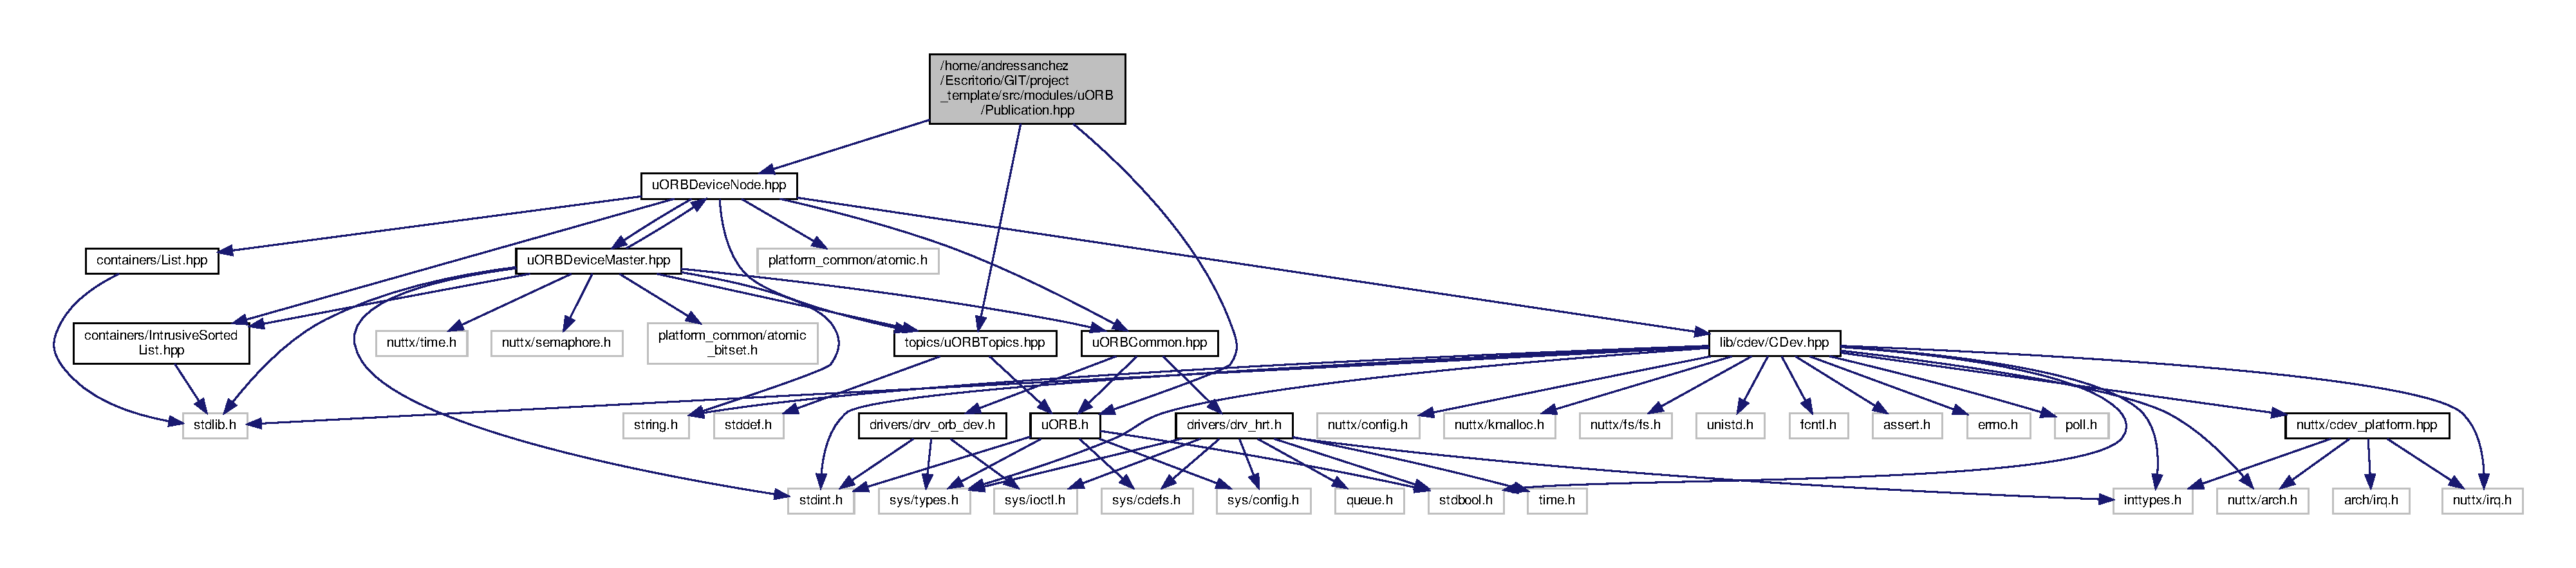
\includegraphics[width=350pt]{d5/d50/Publication_8hpp__incl}
\end{center}
\end{figure}
This graph shows which files directly or indirectly include this file\+:
\nopagebreak
\begin{figure}[H]
\begin{center}
\leavevmode
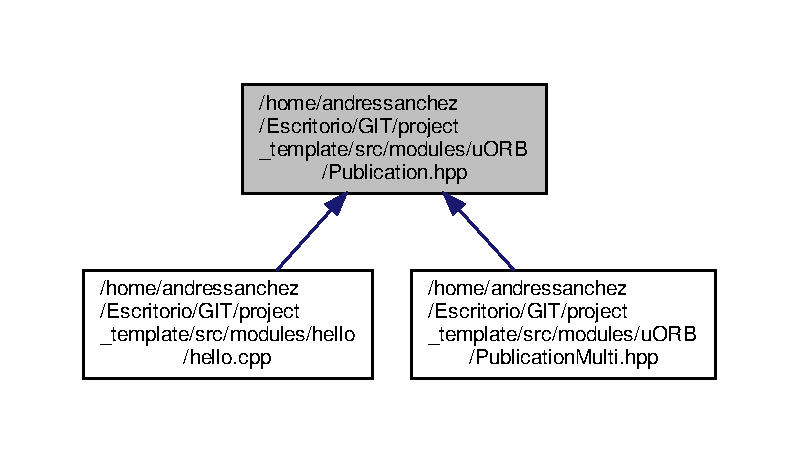
\includegraphics[width=226pt]{d9/dc8/Publication_8hpp__dep__incl}
\end{center}
\end{figure}
\subsection*{Classes}
\begin{DoxyCompactItemize}
\item 
class \hyperlink{classuORB_1_1PublicationBase}{u\+O\+R\+B\+::\+Publication\+Base}
\item 
class \hyperlink{classuORB_1_1Publication}{u\+O\+R\+B\+::\+Publication$<$ T, O\+R\+B\+\_\+\+Q\+S\+I\+Z\+E $>$}
\item 
class \hyperlink{classuORB_1_1PublicationData}{u\+O\+R\+B\+::\+Publication\+Data$<$ T $>$}
\end{DoxyCompactItemize}
\subsection*{Typedefs}
\begin{DoxyCompactItemize}
\item 
\mbox{\Hypertarget{Publication_8hpp_aad492b5beb732cc56353e68a32da7b1e}\label{Publication_8hpp_aad492b5beb732cc56353e68a32da7b1e}} 
{\footnotesize template$<$class T $>$ }\\using {\bfseries u\+O\+R\+B\+::\+Publication\+Queued} = Publication$<$ T, T\+::\+O\+R\+B\+\_\+\+Q\+U\+E\+U\+E\+\_\+\+L\+E\+N\+G\+TH $>$
\end{DoxyCompactItemize}

\hypertarget{Subscription_8cpp}{}\section{/home/andressanchez/\+Escritorio/\+G\+I\+T/project\+\_\+template/src/modules/u\+O\+R\+B/\+Subscription.cpp File Reference}
\label{Subscription_8cpp}\index{/home/andressanchez/\+Escritorio/\+G\+I\+T/project\+\_\+template/src/modules/u\+O\+R\+B/\+Subscription.\+cpp@{/home/andressanchez/\+Escritorio/\+G\+I\+T/project\+\_\+template/src/modules/u\+O\+R\+B/\+Subscription.\+cpp}}
{\ttfamily \#include \char`\"{}Subscription.\+hpp\char`\"{}}\newline
Include dependency graph for Subscription.\+cpp\+:
\nopagebreak
\begin{figure}[H]
\begin{center}
\leavevmode
\includegraphics[width=350pt]{d5/dd5/Subscription_8cpp__incl}
\end{center}
\end{figure}

\hypertarget{Subscription_8hpp}{}\section{/home/andressanchez/\+Escritorio/\+G\+I\+T/project\+\_\+template/src/modules/u\+O\+R\+B/\+Subscription.hpp File Reference}
\label{Subscription_8hpp}\index{/home/andressanchez/\+Escritorio/\+G\+I\+T/project\+\_\+template/src/modules/u\+O\+R\+B/\+Subscription.\+hpp@{/home/andressanchez/\+Escritorio/\+G\+I\+T/project\+\_\+template/src/modules/u\+O\+R\+B/\+Subscription.\+hpp}}
{\ttfamily \#include \char`\"{}u\+O\+R\+B.\+h\char`\"{}}\newline
{\ttfamily \#include \char`\"{}topics/u\+O\+R\+B\+Topics.\+hpp\char`\"{}}\newline
{\ttfamily \#include \char`\"{}u\+O\+R\+B\+Device\+Node.\+hpp\char`\"{}}\newline
{\ttfamily \#include \char`\"{}u\+O\+R\+B\+Manager.\+hpp\char`\"{}}\newline
{\ttfamily \#include \char`\"{}u\+O\+R\+B\+Utils.\+hpp\char`\"{}}\newline
Include dependency graph for Subscription.\+hpp\+:
\nopagebreak
\begin{figure}[H]
\begin{center}
\leavevmode
\includegraphics[width=350pt]{db/dc7/Subscription_8hpp__incl}
\end{center}
\end{figure}
This graph shows which files directly or indirectly include this file\+:
\nopagebreak
\begin{figure}[H]
\begin{center}
\leavevmode
\includegraphics[width=350pt]{d3/d3e/Subscription_8hpp__dep__incl}
\end{center}
\end{figure}
\subsection*{Classes}
\begin{DoxyCompactItemize}
\item 
class \hyperlink{classuORB_1_1Subscription}{u\+O\+R\+B\+::\+Subscription}
\item 
class \hyperlink{classuORB_1_1SubscriptionData}{u\+O\+R\+B\+::\+Subscription\+Data$<$ T $>$}
\end{DoxyCompactItemize}

\hypertarget{SubscriptionCallback_8hpp}{}\section{/home/andressanchez/\+Escritorio/\+G\+I\+T/project\+\_\+template/src/modules/u\+O\+R\+B/\+Subscription\+Callback.hpp File Reference}
\label{SubscriptionCallback_8hpp}\index{/home/andressanchez/\+Escritorio/\+G\+I\+T/project\+\_\+template/src/modules/u\+O\+R\+B/\+Subscription\+Callback.\+hpp@{/home/andressanchez/\+Escritorio/\+G\+I\+T/project\+\_\+template/src/modules/u\+O\+R\+B/\+Subscription\+Callback.\+hpp}}
{\ttfamily \#include \char`\"{}Subscription\+Interval.\+hpp\char`\"{}}\newline
{\ttfamily \#include \char`\"{}include/containers/\+List.\+hpp\char`\"{}}\newline
Include dependency graph for Subscription\+Callback.\+hpp\+:
\nopagebreak
\begin{figure}[H]
\begin{center}
\leavevmode
\includegraphics[width=350pt]{d0/d9c/SubscriptionCallback_8hpp__incl}
\end{center}
\end{figure}
This graph shows which files directly or indirectly include this file\+:
\nopagebreak
\begin{figure}[H]
\begin{center}
\leavevmode
\includegraphics[width=350pt]{d1/d08/SubscriptionCallback_8hpp__dep__incl}
\end{center}
\end{figure}
\subsection*{Classes}
\begin{DoxyCompactItemize}
\item 
class \hyperlink{classuORB_1_1SubscriptionCallback}{u\+O\+R\+B\+::\+Subscription\+Callback}
\end{DoxyCompactItemize}

\hypertarget{SubscriptionInterval_8hpp}{}\section{/home/andressanchez/\+Escritorio/\+G\+I\+T/project\+\_\+template/src/modules/u\+O\+R\+B/\+Subscription\+Interval.hpp File Reference}
\label{SubscriptionInterval_8hpp}\index{/home/andressanchez/\+Escritorio/\+G\+I\+T/project\+\_\+template/src/modules/u\+O\+R\+B/\+Subscription\+Interval.\+hpp@{/home/andressanchez/\+Escritorio/\+G\+I\+T/project\+\_\+template/src/modules/u\+O\+R\+B/\+Subscription\+Interval.\+hpp}}
{\ttfamily \#include \char`\"{}u\+O\+R\+B.\+h\char`\"{}}\newline
{\ttfamily \#include \char`\"{}u\+O\+R\+B\+Device\+Node.\+hpp\char`\"{}}\newline
{\ttfamily \#include \char`\"{}u\+O\+R\+B\+Manager.\+hpp\char`\"{}}\newline
{\ttfamily \#include \char`\"{}u\+O\+R\+B\+Utils.\+hpp\char`\"{}}\newline
{\ttfamily \#include \char`\"{}Subscription.\+hpp\char`\"{}}\newline
{\ttfamily \#include \char`\"{}include/\+Limits.\+hpp\char`\"{}}\newline
Include dependency graph for Subscription\+Interval.\+hpp\+:
\nopagebreak
\begin{figure}[H]
\begin{center}
\leavevmode
\includegraphics[width=350pt]{db/d9a/SubscriptionInterval_8hpp__incl}
\end{center}
\end{figure}
This graph shows which files directly or indirectly include this file\+:
\nopagebreak
\begin{figure}[H]
\begin{center}
\leavevmode
\includegraphics[width=350pt]{d0/d04/SubscriptionInterval_8hpp__dep__incl}
\end{center}
\end{figure}
\subsection*{Classes}
\begin{DoxyCompactItemize}
\item 
class \hyperlink{classuORB_1_1SubscriptionInterval}{u\+O\+R\+B\+::\+Subscription\+Interval}
\end{DoxyCompactItemize}

\hypertarget{SubscriptionMultiArray_8hpp}{}\section{/home/andressanchez/\+Escritorio/\+G\+I\+T/project\+\_\+template/src/modules/u\+O\+R\+B/\+Subscription\+Multi\+Array.hpp File Reference}
\label{SubscriptionMultiArray_8hpp}\index{/home/andressanchez/\+Escritorio/\+G\+I\+T/project\+\_\+template/src/modules/u\+O\+R\+B/\+Subscription\+Multi\+Array.\+hpp@{/home/andressanchez/\+Escritorio/\+G\+I\+T/project\+\_\+template/src/modules/u\+O\+R\+B/\+Subscription\+Multi\+Array.\+hpp}}
{\ttfamily \#include \char`\"{}u\+O\+R\+B.\+h\char`\"{}}\newline
{\ttfamily \#include \char`\"{}Subscription\+Interval.\+hpp\char`\"{}}\newline
Include dependency graph for Subscription\+Multi\+Array.\+hpp\+:
\nopagebreak
\begin{figure}[H]
\begin{center}
\leavevmode
\includegraphics[width=350pt]{db/d58/SubscriptionMultiArray_8hpp__incl}
\end{center}
\end{figure}
\subsection*{Classes}
\begin{DoxyCompactItemize}
\item 
class \hyperlink{classuORB_1_1SubscriptionMultiArray}{u\+O\+R\+B\+::\+Subscription\+Multi\+Array$<$ T, S\+I\+Z\+E $>$}
\end{DoxyCompactItemize}

\hypertarget{uORB_8cpp}{}\section{/home/andressanchez/\+Escritorio/\+G\+I\+T/project\+\_\+template/src/modules/u\+O\+R\+B/u\+O\+RB.cpp File Reference}
\label{uORB_8cpp}\index{/home/andressanchez/\+Escritorio/\+G\+I\+T/project\+\_\+template/src/modules/u\+O\+R\+B/u\+O\+R\+B.\+cpp@{/home/andressanchez/\+Escritorio/\+G\+I\+T/project\+\_\+template/src/modules/u\+O\+R\+B/u\+O\+R\+B.\+cpp}}
{\ttfamily \#include \char`\"{}u\+O\+R\+B.\+h\char`\"{}}\newline
{\ttfamily \#include \char`\"{}u\+O\+R\+B\+Manager.\+hpp\char`\"{}}\newline
{\ttfamily \#include \char`\"{}u\+O\+R\+B\+Common.\+hpp\char`\"{}}\newline
Include dependency graph for u\+O\+R\+B.\+cpp\+:
\nopagebreak
\begin{figure}[H]
\begin{center}
\leavevmode
\includegraphics[width=350pt]{d1/dd5/uORB_8cpp__incl}
\end{center}
\end{figure}
\subsection*{Functions}
\begin{DoxyCompactItemize}
\item 
\hyperlink{uORB_8h_a8d0cfa5f9ea6427a37057d6cea6dd990}{orb\+\_\+advert\+\_\+t} \hyperlink{uORB_8cpp_ac5ba0a0d1dc62f813314c0ff37a9a82a}{orb\+\_\+advertise} (const struct \hyperlink{structorb__metadata}{orb\+\_\+metadata} $\ast$meta, const void $\ast$data)
\item 
\hyperlink{uORB_8h_a8d0cfa5f9ea6427a37057d6cea6dd990}{orb\+\_\+advert\+\_\+t} \hyperlink{uORB_8cpp_a91df70141220b84c1c01619db0c3e105}{orb\+\_\+advertise\+\_\+queue} (const struct \hyperlink{structorb__metadata}{orb\+\_\+metadata} $\ast$meta, const void $\ast$data, unsigned int queue\+\_\+size)
\item 
\hyperlink{uORB_8h_a8d0cfa5f9ea6427a37057d6cea6dd990}{orb\+\_\+advert\+\_\+t} \hyperlink{uORB_8cpp_abe388f04be634866674331bb88664597}{orb\+\_\+advertise\+\_\+multi} (const struct \hyperlink{structorb__metadata}{orb\+\_\+metadata} $\ast$meta, const void $\ast$data, int $\ast$instance)
\item 
\hyperlink{uORB_8h_a8d0cfa5f9ea6427a37057d6cea6dd990}{orb\+\_\+advert\+\_\+t} \hyperlink{uORB_8cpp_a858116e979c705acb7c551a9649b0fec}{orb\+\_\+advertise\+\_\+multi\+\_\+queue} (const struct \hyperlink{structorb__metadata}{orb\+\_\+metadata} $\ast$meta, const void $\ast$data, int $\ast$instance, unsigned int queue\+\_\+size)
\item 
int \hyperlink{uORB_8cpp_a1c2ecd4919751835265681c212badaf4}{orb\+\_\+unadvertise} (\hyperlink{uORB_8h_a8d0cfa5f9ea6427a37057d6cea6dd990}{orb\+\_\+advert\+\_\+t} handle)
\item 
int \hyperlink{uORB_8cpp_af7a143a80b6b04689a3a4890ce8df4ae}{orb\+\_\+publish} (const struct \hyperlink{structorb__metadata}{orb\+\_\+metadata} $\ast$meta, \hyperlink{uORB_8h_a8d0cfa5f9ea6427a37057d6cea6dd990}{orb\+\_\+advert\+\_\+t} handle, const void $\ast$data)
\item 
int \hyperlink{uORB_8cpp_a196a292b740589eff958aa42c4e96ef5}{orb\+\_\+subscribe} (const struct \hyperlink{structorb__metadata}{orb\+\_\+metadata} $\ast$meta)
\item 
int \hyperlink{uORB_8cpp_a2c71c73d77220ff8faf2cb8eb7509e66}{orb\+\_\+subscribe\+\_\+multi} (const struct \hyperlink{structorb__metadata}{orb\+\_\+metadata} $\ast$meta, unsigned instance)
\item 
int \hyperlink{uORB_8cpp_a8adc3c48c1860deac8bd2a520e391837}{orb\+\_\+unsubscribe} (int handle)
\item 
int \hyperlink{uORB_8cpp_a2c09f842c44c64a06bcfe7a921f63cdf}{orb\+\_\+copy} (const struct \hyperlink{structorb__metadata}{orb\+\_\+metadata} $\ast$meta, int handle, void $\ast$buffer)
\item 
int \hyperlink{uORB_8cpp_a29b31278909062127ba89245a8182706}{orb\+\_\+check} (int handle, bool $\ast$updated)
\item 
int \hyperlink{uORB_8cpp_a840e123b2492357b5a302b7a867b8916}{orb\+\_\+exists} (const struct \hyperlink{structorb__metadata}{orb\+\_\+metadata} $\ast$meta, int instance)
\item 
int \hyperlink{uORB_8cpp_a10876a56e0054909b8e40fedd8baa624}{orb\+\_\+group\+\_\+count} (const struct \hyperlink{structorb__metadata}{orb\+\_\+metadata} $\ast$meta)
\item 
int \hyperlink{uORB_8cpp_a5ddf366cd5c691af0d027c0bc0b173ba}{orb\+\_\+set\+\_\+interval} (int handle, unsigned interval)
\item 
int \hyperlink{uORB_8cpp_ae277b3d3a49ba3379134c4d49b43ab45}{orb\+\_\+get\+\_\+interval} (int handle, unsigned $\ast$interval)
\end{DoxyCompactItemize}


\subsection{Detailed Description}
A lightweight object broker. 

\subsection{Function Documentation}
\mbox{\Hypertarget{uORB_8cpp_ac5ba0a0d1dc62f813314c0ff37a9a82a}\label{uORB_8cpp_ac5ba0a0d1dc62f813314c0ff37a9a82a}} 
\index{u\+O\+R\+B.\+cpp@{u\+O\+R\+B.\+cpp}!orb\+\_\+advertise@{orb\+\_\+advertise}}
\index{orb\+\_\+advertise@{orb\+\_\+advertise}!u\+O\+R\+B.\+cpp@{u\+O\+R\+B.\+cpp}}
\subsubsection{\texorpdfstring{orb\+\_\+advertise()}{orb\_advertise()}}
{\footnotesize\ttfamily \hyperlink{uORB_8h_a8d0cfa5f9ea6427a37057d6cea6dd990}{orb\+\_\+advert\+\_\+t} orb\+\_\+advertise (\begin{DoxyParamCaption}\item[{const struct \hyperlink{structorb__metadata}{orb\+\_\+metadata} $\ast$}]{meta,  }\item[{const void $\ast$}]{data }\end{DoxyParamCaption})}

\begin{DoxySeeAlso}{See also}
\hyperlink{classuORB_1_1Manager_a42e075fba5970aa0730faab182e2083f}{u\+O\+R\+B\+::\+Manager\+::orb\+\_\+advertise()} 
\end{DoxySeeAlso}


Definition at line 43 of file u\+O\+R\+B.\+cpp.


\begin{DoxyCode}
44 \{
45     \textcolor{keywordflow}{return} \hyperlink{classuORB_1_1Manager_a9d829b3ea49d16d03c2fa37ef2bb24a5}{uORB::Manager::get\_instance}()->
      \hyperlink{classuORB_1_1Manager_a42e075fba5970aa0730faab182e2083f}{orb\_advertise}(meta, data);
46 \}
\end{DoxyCode}
\mbox{\Hypertarget{uORB_8cpp_abe388f04be634866674331bb88664597}\label{uORB_8cpp_abe388f04be634866674331bb88664597}} 
\index{u\+O\+R\+B.\+cpp@{u\+O\+R\+B.\+cpp}!orb\+\_\+advertise\+\_\+multi@{orb\+\_\+advertise\+\_\+multi}}
\index{orb\+\_\+advertise\+\_\+multi@{orb\+\_\+advertise\+\_\+multi}!u\+O\+R\+B.\+cpp@{u\+O\+R\+B.\+cpp}}
\subsubsection{\texorpdfstring{orb\+\_\+advertise\+\_\+multi()}{orb\_advertise\_multi()}}
{\footnotesize\ttfamily \hyperlink{uORB_8h_a8d0cfa5f9ea6427a37057d6cea6dd990}{orb\+\_\+advert\+\_\+t} orb\+\_\+advertise\+\_\+multi (\begin{DoxyParamCaption}\item[{const struct \hyperlink{structorb__metadata}{orb\+\_\+metadata} $\ast$}]{meta,  }\item[{const void $\ast$}]{data,  }\item[{int $\ast$}]{instance }\end{DoxyParamCaption})}

\begin{DoxySeeAlso}{See also}
\hyperlink{classuORB_1_1Manager_a808104f7ebeab8f0d548dd9127344b24}{u\+O\+R\+B\+::\+Manager\+::orb\+\_\+advertise\+\_\+multi()} 
\end{DoxySeeAlso}


Definition at line 53 of file u\+O\+R\+B.\+cpp.


\begin{DoxyCode}
54 \{
55     \textcolor{keywordflow}{return} \hyperlink{classuORB_1_1Manager_a9d829b3ea49d16d03c2fa37ef2bb24a5}{uORB::Manager::get\_instance}()->
      \hyperlink{classuORB_1_1Manager_a808104f7ebeab8f0d548dd9127344b24}{orb\_advertise\_multi}(meta, data, instance);
56 \}
\end{DoxyCode}
\mbox{\Hypertarget{uORB_8cpp_a858116e979c705acb7c551a9649b0fec}\label{uORB_8cpp_a858116e979c705acb7c551a9649b0fec}} 
\index{u\+O\+R\+B.\+cpp@{u\+O\+R\+B.\+cpp}!orb\+\_\+advertise\+\_\+multi\+\_\+queue@{orb\+\_\+advertise\+\_\+multi\+\_\+queue}}
\index{orb\+\_\+advertise\+\_\+multi\+\_\+queue@{orb\+\_\+advertise\+\_\+multi\+\_\+queue}!u\+O\+R\+B.\+cpp@{u\+O\+R\+B.\+cpp}}
\subsubsection{\texorpdfstring{orb\+\_\+advertise\+\_\+multi\+\_\+queue()}{orb\_advertise\_multi\_queue()}}
{\footnotesize\ttfamily \hyperlink{uORB_8h_a8d0cfa5f9ea6427a37057d6cea6dd990}{orb\+\_\+advert\+\_\+t} orb\+\_\+advertise\+\_\+multi\+\_\+queue (\begin{DoxyParamCaption}\item[{const struct \hyperlink{structorb__metadata}{orb\+\_\+metadata} $\ast$}]{meta,  }\item[{const void $\ast$}]{data,  }\item[{int $\ast$}]{instance,  }\item[{unsigned int}]{queue\+\_\+size }\end{DoxyParamCaption})}

\begin{DoxySeeAlso}{See also}
\hyperlink{classuORB_1_1Manager_a808104f7ebeab8f0d548dd9127344b24}{u\+O\+R\+B\+::\+Manager\+::orb\+\_\+advertise\+\_\+multi()} 
\end{DoxySeeAlso}


Definition at line 58 of file u\+O\+R\+B.\+cpp.


\begin{DoxyCode}
60 \{
61     \textcolor{keywordflow}{return} \hyperlink{classuORB_1_1Manager_a9d829b3ea49d16d03c2fa37ef2bb24a5}{uORB::Manager::get\_instance}()->
      \hyperlink{classuORB_1_1Manager_a808104f7ebeab8f0d548dd9127344b24}{orb\_advertise\_multi}(meta, data, instance, queue\_size);
62 \}
\end{DoxyCode}
\mbox{\Hypertarget{uORB_8cpp_a91df70141220b84c1c01619db0c3e105}\label{uORB_8cpp_a91df70141220b84c1c01619db0c3e105}} 
\index{u\+O\+R\+B.\+cpp@{u\+O\+R\+B.\+cpp}!orb\+\_\+advertise\+\_\+queue@{orb\+\_\+advertise\+\_\+queue}}
\index{orb\+\_\+advertise\+\_\+queue@{orb\+\_\+advertise\+\_\+queue}!u\+O\+R\+B.\+cpp@{u\+O\+R\+B.\+cpp}}
\subsubsection{\texorpdfstring{orb\+\_\+advertise\+\_\+queue()}{orb\_advertise\_queue()}}
{\footnotesize\ttfamily \hyperlink{uORB_8h_a8d0cfa5f9ea6427a37057d6cea6dd990}{orb\+\_\+advert\+\_\+t} orb\+\_\+advertise\+\_\+queue (\begin{DoxyParamCaption}\item[{const struct \hyperlink{structorb__metadata}{orb\+\_\+metadata} $\ast$}]{meta,  }\item[{const void $\ast$}]{data,  }\item[{unsigned int}]{queue\+\_\+size }\end{DoxyParamCaption})}

\begin{DoxySeeAlso}{See also}
\hyperlink{classuORB_1_1Manager_a42e075fba5970aa0730faab182e2083f}{u\+O\+R\+B\+::\+Manager\+::orb\+\_\+advertise()} 
\end{DoxySeeAlso}


Definition at line 48 of file u\+O\+R\+B.\+cpp.


\begin{DoxyCode}
49 \{
50     \textcolor{keywordflow}{return} \hyperlink{classuORB_1_1Manager_a9d829b3ea49d16d03c2fa37ef2bb24a5}{uORB::Manager::get\_instance}()->
      \hyperlink{classuORB_1_1Manager_a42e075fba5970aa0730faab182e2083f}{orb\_advertise}(meta, data, queue\_size);
51 \}
\end{DoxyCode}
\mbox{\Hypertarget{uORB_8cpp_a29b31278909062127ba89245a8182706}\label{uORB_8cpp_a29b31278909062127ba89245a8182706}} 
\index{u\+O\+R\+B.\+cpp@{u\+O\+R\+B.\+cpp}!orb\+\_\+check@{orb\+\_\+check}}
\index{orb\+\_\+check@{orb\+\_\+check}!u\+O\+R\+B.\+cpp@{u\+O\+R\+B.\+cpp}}
\subsubsection{\texorpdfstring{orb\+\_\+check()}{orb\_check()}}
{\footnotesize\ttfamily int orb\+\_\+check (\begin{DoxyParamCaption}\item[{int}]{handle,  }\item[{bool $\ast$}]{updated }\end{DoxyParamCaption})}

\begin{DoxySeeAlso}{See also}
\hyperlink{classuORB_1_1Manager_a5503920d25d544ce3be1cf79cda869f7}{u\+O\+R\+B\+::\+Manager\+::orb\+\_\+check()} 
\end{DoxySeeAlso}


Definition at line 94 of file u\+O\+R\+B.\+cpp.


\begin{DoxyCode}
95 \{
96     \textcolor{keywordflow}{return} \hyperlink{classuORB_1_1Manager_a9d829b3ea49d16d03c2fa37ef2bb24a5}{uORB::Manager::get\_instance}()->\hyperlink{classuORB_1_1Manager_a5503920d25d544ce3be1cf79cda869f7}{orb\_check}(handle, updated);
97 \}
\end{DoxyCode}
\mbox{\Hypertarget{uORB_8cpp_a2c09f842c44c64a06bcfe7a921f63cdf}\label{uORB_8cpp_a2c09f842c44c64a06bcfe7a921f63cdf}} 
\index{u\+O\+R\+B.\+cpp@{u\+O\+R\+B.\+cpp}!orb\+\_\+copy@{orb\+\_\+copy}}
\index{orb\+\_\+copy@{orb\+\_\+copy}!u\+O\+R\+B.\+cpp@{u\+O\+R\+B.\+cpp}}
\subsubsection{\texorpdfstring{orb\+\_\+copy()}{orb\_copy()}}
{\footnotesize\ttfamily int orb\+\_\+copy (\begin{DoxyParamCaption}\item[{const struct \hyperlink{structorb__metadata}{orb\+\_\+metadata} $\ast$}]{meta,  }\item[{int}]{handle,  }\item[{void $\ast$}]{buffer }\end{DoxyParamCaption})}

\begin{DoxySeeAlso}{See also}
\hyperlink{classuORB_1_1Manager_af1048c82b439300c706fe0a083b61f90}{u\+O\+R\+B\+::\+Manager\+::orb\+\_\+copy()} 
\end{DoxySeeAlso}


Definition at line 89 of file u\+O\+R\+B.\+cpp.


\begin{DoxyCode}
90 \{
91     \textcolor{keywordflow}{return} \hyperlink{classuORB_1_1Manager_a9d829b3ea49d16d03c2fa37ef2bb24a5}{uORB::Manager::get\_instance}()->\hyperlink{classuORB_1_1Manager_af1048c82b439300c706fe0a083b61f90}{orb\_copy}(meta, handle, buffer)
      ;
92 \}
\end{DoxyCode}
\mbox{\Hypertarget{uORB_8cpp_a840e123b2492357b5a302b7a867b8916}\label{uORB_8cpp_a840e123b2492357b5a302b7a867b8916}} 
\index{u\+O\+R\+B.\+cpp@{u\+O\+R\+B.\+cpp}!orb\+\_\+exists@{orb\+\_\+exists}}
\index{orb\+\_\+exists@{orb\+\_\+exists}!u\+O\+R\+B.\+cpp@{u\+O\+R\+B.\+cpp}}
\subsubsection{\texorpdfstring{orb\+\_\+exists()}{orb\_exists()}}
{\footnotesize\ttfamily int orb\+\_\+exists (\begin{DoxyParamCaption}\item[{const struct \hyperlink{structorb__metadata}{orb\+\_\+metadata} $\ast$}]{meta,  }\item[{int}]{instance }\end{DoxyParamCaption})}

\begin{DoxySeeAlso}{See also}
\hyperlink{classuORB_1_1Manager_a446823738a75847a6732008784445c9f}{u\+O\+R\+B\+::\+Manager\+::orb\+\_\+exists()} 
\end{DoxySeeAlso}


Definition at line 99 of file u\+O\+R\+B.\+cpp.


\begin{DoxyCode}
100 \{
101     \textcolor{keywordflow}{return} \hyperlink{classuORB_1_1Manager_a9d829b3ea49d16d03c2fa37ef2bb24a5}{uORB::Manager::get\_instance}()->\hyperlink{classuORB_1_1Manager_a446823738a75847a6732008784445c9f}{orb\_exists}(meta, instance);
102 \}
\end{DoxyCode}
\mbox{\Hypertarget{uORB_8cpp_ae277b3d3a49ba3379134c4d49b43ab45}\label{uORB_8cpp_ae277b3d3a49ba3379134c4d49b43ab45}} 
\index{u\+O\+R\+B.\+cpp@{u\+O\+R\+B.\+cpp}!orb\+\_\+get\+\_\+interval@{orb\+\_\+get\+\_\+interval}}
\index{orb\+\_\+get\+\_\+interval@{orb\+\_\+get\+\_\+interval}!u\+O\+R\+B.\+cpp@{u\+O\+R\+B.\+cpp}}
\subsubsection{\texorpdfstring{orb\+\_\+get\+\_\+interval()}{orb\_get\_interval()}}
{\footnotesize\ttfamily int orb\+\_\+get\+\_\+interval (\begin{DoxyParamCaption}\item[{int}]{handle,  }\item[{unsigned $\ast$}]{interval }\end{DoxyParamCaption})}

\begin{DoxySeeAlso}{See also}
\hyperlink{classuORB_1_1Manager_a627a7e6ef16970d2b6d8f02471795963}{u\+O\+R\+B\+::\+Manager\+::orb\+\_\+get\+\_\+interval()} 
\end{DoxySeeAlso}


Definition at line 120 of file u\+O\+R\+B.\+cpp.


\begin{DoxyCode}
121 \{
122     \textcolor{keywordflow}{return} \hyperlink{classuORB_1_1Manager_a9d829b3ea49d16d03c2fa37ef2bb24a5}{uORB::Manager::get\_instance}()->
      \hyperlink{classuORB_1_1Manager_a627a7e6ef16970d2b6d8f02471795963}{orb\_get\_interval}(handle, interval);
123 \}
\end{DoxyCode}
\mbox{\Hypertarget{uORB_8cpp_a10876a56e0054909b8e40fedd8baa624}\label{uORB_8cpp_a10876a56e0054909b8e40fedd8baa624}} 
\index{u\+O\+R\+B.\+cpp@{u\+O\+R\+B.\+cpp}!orb\+\_\+group\+\_\+count@{orb\+\_\+group\+\_\+count}}
\index{orb\+\_\+group\+\_\+count@{orb\+\_\+group\+\_\+count}!u\+O\+R\+B.\+cpp@{u\+O\+R\+B.\+cpp}}
\subsubsection{\texorpdfstring{orb\+\_\+group\+\_\+count()}{orb\_group\_count()}}
{\footnotesize\ttfamily int orb\+\_\+group\+\_\+count (\begin{DoxyParamCaption}\item[{const struct \hyperlink{structorb__metadata}{orb\+\_\+metadata} $\ast$}]{meta }\end{DoxyParamCaption})}

Get the number of published instances of a topic group


\begin{DoxyParams}{Parameters}
{\em meta} & O\+RB topic metadata. \\
\hline
\end{DoxyParams}
\begin{DoxyReturn}{Returns}
The number of published instances of this topic 
\end{DoxyReturn}


Definition at line 104 of file u\+O\+R\+B.\+cpp.


\begin{DoxyCode}
105 \{
106     \textcolor{keywordtype}{unsigned} instance = 0;
107 
108     \textcolor{keywordflow}{while} (\hyperlink{classuORB_1_1Manager_a9d829b3ea49d16d03c2fa37ef2bb24a5}{uORB::Manager::get\_instance}()->\hyperlink{uORB_8cpp_a840e123b2492357b5a302b7a867b8916}{orb\_exists}(meta, instance) 
      == 0) \{
109         ++instance;
110     \};
111 
112     \textcolor{keywordflow}{return} instance;
113 \}
\end{DoxyCode}
\mbox{\Hypertarget{uORB_8cpp_af7a143a80b6b04689a3a4890ce8df4ae}\label{uORB_8cpp_af7a143a80b6b04689a3a4890ce8df4ae}} 
\index{u\+O\+R\+B.\+cpp@{u\+O\+R\+B.\+cpp}!orb\+\_\+publish@{orb\+\_\+publish}}
\index{orb\+\_\+publish@{orb\+\_\+publish}!u\+O\+R\+B.\+cpp@{u\+O\+R\+B.\+cpp}}
\subsubsection{\texorpdfstring{orb\+\_\+publish()}{orb\_publish()}}
{\footnotesize\ttfamily int orb\+\_\+publish (\begin{DoxyParamCaption}\item[{const struct \hyperlink{structorb__metadata}{orb\+\_\+metadata} $\ast$}]{meta,  }\item[{\hyperlink{uORB_8h_a8d0cfa5f9ea6427a37057d6cea6dd990}{orb\+\_\+advert\+\_\+t}}]{handle,  }\item[{const void $\ast$}]{data }\end{DoxyParamCaption})}

\begin{DoxySeeAlso}{See also}
\hyperlink{classuORB_1_1Manager_abbe6966f841886ce3003ebc6d2198447}{u\+O\+R\+B\+::\+Manager\+::orb\+\_\+publish()} 
\end{DoxySeeAlso}


Definition at line 69 of file u\+O\+R\+B.\+cpp.


\begin{DoxyCode}
70 \{
71     \textcolor{keywordflow}{return} \hyperlink{classuORB_1_1Manager_a9d829b3ea49d16d03c2fa37ef2bb24a5}{uORB::Manager::get\_instance}()->\hyperlink{classuORB_1_1Manager_abbe6966f841886ce3003ebc6d2198447}{orb\_publish}(meta, handle, 
      data);
72 \}
\end{DoxyCode}
\mbox{\Hypertarget{uORB_8cpp_a5ddf366cd5c691af0d027c0bc0b173ba}\label{uORB_8cpp_a5ddf366cd5c691af0d027c0bc0b173ba}} 
\index{u\+O\+R\+B.\+cpp@{u\+O\+R\+B.\+cpp}!orb\+\_\+set\+\_\+interval@{orb\+\_\+set\+\_\+interval}}
\index{orb\+\_\+set\+\_\+interval@{orb\+\_\+set\+\_\+interval}!u\+O\+R\+B.\+cpp@{u\+O\+R\+B.\+cpp}}
\subsubsection{\texorpdfstring{orb\+\_\+set\+\_\+interval()}{orb\_set\_interval()}}
{\footnotesize\ttfamily int orb\+\_\+set\+\_\+interval (\begin{DoxyParamCaption}\item[{int}]{handle,  }\item[{unsigned}]{interval }\end{DoxyParamCaption})}

\begin{DoxySeeAlso}{See also}
\hyperlink{classuORB_1_1Manager_aade04ff2a8a3aaf275b39fc32934fc56}{u\+O\+R\+B\+::\+Manager\+::orb\+\_\+set\+\_\+interval()} 
\end{DoxySeeAlso}


Definition at line 115 of file u\+O\+R\+B.\+cpp.


\begin{DoxyCode}
116 \{
117     \textcolor{keywordflow}{return} \hyperlink{classuORB_1_1Manager_a9d829b3ea49d16d03c2fa37ef2bb24a5}{uORB::Manager::get\_instance}()->
      \hyperlink{classuORB_1_1Manager_aade04ff2a8a3aaf275b39fc32934fc56}{orb\_set\_interval}(handle, interval);
118 \}
\end{DoxyCode}
\mbox{\Hypertarget{uORB_8cpp_a196a292b740589eff958aa42c4e96ef5}\label{uORB_8cpp_a196a292b740589eff958aa42c4e96ef5}} 
\index{u\+O\+R\+B.\+cpp@{u\+O\+R\+B.\+cpp}!orb\+\_\+subscribe@{orb\+\_\+subscribe}}
\index{orb\+\_\+subscribe@{orb\+\_\+subscribe}!u\+O\+R\+B.\+cpp@{u\+O\+R\+B.\+cpp}}
\subsubsection{\texorpdfstring{orb\+\_\+subscribe()}{orb\_subscribe()}}
{\footnotesize\ttfamily int orb\+\_\+subscribe (\begin{DoxyParamCaption}\item[{const struct \hyperlink{structorb__metadata}{orb\+\_\+metadata} $\ast$}]{meta }\end{DoxyParamCaption})}

\begin{DoxySeeAlso}{See also}
\hyperlink{classuORB_1_1Manager_ae54072a80ad4de6d127e2dad8182b8fb}{u\+O\+R\+B\+::\+Manager\+::orb\+\_\+subscribe()} 
\end{DoxySeeAlso}


Definition at line 74 of file u\+O\+R\+B.\+cpp.


\begin{DoxyCode}
75 \{
76     \textcolor{keywordflow}{return} \hyperlink{classuORB_1_1Manager_a9d829b3ea49d16d03c2fa37ef2bb24a5}{uORB::Manager::get\_instance}()->
      \hyperlink{classuORB_1_1Manager_ae54072a80ad4de6d127e2dad8182b8fb}{orb\_subscribe}(meta);
77 \}
\end{DoxyCode}
\mbox{\Hypertarget{uORB_8cpp_a2c71c73d77220ff8faf2cb8eb7509e66}\label{uORB_8cpp_a2c71c73d77220ff8faf2cb8eb7509e66}} 
\index{u\+O\+R\+B.\+cpp@{u\+O\+R\+B.\+cpp}!orb\+\_\+subscribe\+\_\+multi@{orb\+\_\+subscribe\+\_\+multi}}
\index{orb\+\_\+subscribe\+\_\+multi@{orb\+\_\+subscribe\+\_\+multi}!u\+O\+R\+B.\+cpp@{u\+O\+R\+B.\+cpp}}
\subsubsection{\texorpdfstring{orb\+\_\+subscribe\+\_\+multi()}{orb\_subscribe\_multi()}}
{\footnotesize\ttfamily int orb\+\_\+subscribe\+\_\+multi (\begin{DoxyParamCaption}\item[{const struct \hyperlink{structorb__metadata}{orb\+\_\+metadata} $\ast$}]{meta,  }\item[{unsigned}]{instance }\end{DoxyParamCaption})}

\begin{DoxySeeAlso}{See also}
\hyperlink{classuORB_1_1Manager_a9a31fb71a0962db44450963559296cfe}{u\+O\+R\+B\+::\+Manager\+::orb\+\_\+subscribe\+\_\+multi()} 
\end{DoxySeeAlso}


Definition at line 79 of file u\+O\+R\+B.\+cpp.


\begin{DoxyCode}
80 \{
81     \textcolor{keywordflow}{return} \hyperlink{classuORB_1_1Manager_a9d829b3ea49d16d03c2fa37ef2bb24a5}{uORB::Manager::get\_instance}()->
      \hyperlink{classuORB_1_1Manager_a9a31fb71a0962db44450963559296cfe}{orb\_subscribe\_multi}(meta, instance);
82 \}
\end{DoxyCode}
\mbox{\Hypertarget{uORB_8cpp_a1c2ecd4919751835265681c212badaf4}\label{uORB_8cpp_a1c2ecd4919751835265681c212badaf4}} 
\index{u\+O\+R\+B.\+cpp@{u\+O\+R\+B.\+cpp}!orb\+\_\+unadvertise@{orb\+\_\+unadvertise}}
\index{orb\+\_\+unadvertise@{orb\+\_\+unadvertise}!u\+O\+R\+B.\+cpp@{u\+O\+R\+B.\+cpp}}
\subsubsection{\texorpdfstring{orb\+\_\+unadvertise()}{orb\_unadvertise()}}
{\footnotesize\ttfamily int orb\+\_\+unadvertise (\begin{DoxyParamCaption}\item[{\hyperlink{uORB_8h_a8d0cfa5f9ea6427a37057d6cea6dd990}{orb\+\_\+advert\+\_\+t}}]{handle }\end{DoxyParamCaption})}

\begin{DoxySeeAlso}{See also}
\hyperlink{classuORB_1_1Manager_a45601ddc722320b9cd660d9548263824}{u\+O\+R\+B\+::\+Manager\+::orb\+\_\+unadvertise()} 
\end{DoxySeeAlso}


Definition at line 64 of file u\+O\+R\+B.\+cpp.


\begin{DoxyCode}
65 \{
66     \textcolor{keywordflow}{return} \hyperlink{classuORB_1_1Manager_a9d829b3ea49d16d03c2fa37ef2bb24a5}{uORB::Manager::get\_instance}()->
      \hyperlink{classuORB_1_1Manager_a45601ddc722320b9cd660d9548263824}{orb\_unadvertise}(handle);
67 \}
\end{DoxyCode}
\mbox{\Hypertarget{uORB_8cpp_a8adc3c48c1860deac8bd2a520e391837}\label{uORB_8cpp_a8adc3c48c1860deac8bd2a520e391837}} 
\index{u\+O\+R\+B.\+cpp@{u\+O\+R\+B.\+cpp}!orb\+\_\+unsubscribe@{orb\+\_\+unsubscribe}}
\index{orb\+\_\+unsubscribe@{orb\+\_\+unsubscribe}!u\+O\+R\+B.\+cpp@{u\+O\+R\+B.\+cpp}}
\subsubsection{\texorpdfstring{orb\+\_\+unsubscribe()}{orb\_unsubscribe()}}
{\footnotesize\ttfamily int orb\+\_\+unsubscribe (\begin{DoxyParamCaption}\item[{int}]{handle }\end{DoxyParamCaption})}

\begin{DoxySeeAlso}{See also}
\hyperlink{classuORB_1_1Manager_a77539878280b749d79d2c16dc5628c81}{u\+O\+R\+B\+::\+Manager\+::orb\+\_\+unsubscribe()} 
\end{DoxySeeAlso}


Definition at line 84 of file u\+O\+R\+B.\+cpp.


\begin{DoxyCode}
85 \{
86     \textcolor{keywordflow}{return} \hyperlink{classuORB_1_1Manager_a9d829b3ea49d16d03c2fa37ef2bb24a5}{uORB::Manager::get\_instance}()->
      \hyperlink{classuORB_1_1Manager_a77539878280b749d79d2c16dc5628c81}{orb\_unsubscribe}(handle);
87 \}
\end{DoxyCode}

\hypertarget{uORB_8h}{}\section{/home/andressanchez/\+Escritorio/\+G\+I\+T/project\+\_\+template/src/modules/u\+O\+R\+B/u\+O\+RB.h File Reference}
\label{uORB_8h}\index{/home/andressanchez/\+Escritorio/\+G\+I\+T/project\+\_\+template/src/modules/u\+O\+R\+B/u\+O\+R\+B.\+h@{/home/andressanchez/\+Escritorio/\+G\+I\+T/project\+\_\+template/src/modules/u\+O\+R\+B/u\+O\+R\+B.\+h}}
{\ttfamily \#include $<$sys/config.\+h$>$}\newline
{\ttfamily \#include $<$sys/types.\+h$>$}\newline
{\ttfamily \#include $<$sys/cdefs.\+h$>$}\newline
{\ttfamily \#include $<$stdint.\+h$>$}\newline
{\ttfamily \#include $<$stdbool.\+h$>$}\newline
Include dependency graph for u\+O\+R\+B.\+h\+:\nopagebreak
\begin{figure}[H]
\begin{center}
\leavevmode
\includegraphics[width=350pt]{de/db7/uORB_8h__incl}
\end{center}
\end{figure}
This graph shows which files directly or indirectly include this file\+:\nopagebreak
\begin{figure}[H]
\begin{center}
\leavevmode
\includegraphics[width=350pt]{d9/daa/uORB_8h__dep__incl}
\end{center}
\end{figure}
\subsection*{Classes}
\begin{DoxyCompactItemize}
\item 
struct \hyperlink{structorb__metadata}{orb\+\_\+metadata}
\end{DoxyCompactItemize}
\subsection*{Macros}
\begin{DoxyCompactItemize}
\item 
\#define \hyperlink{uORB_8h_a8c09e8f28a090e8cae61e10d627f102a}{O\+R\+B\+\_\+\+M\+U\+L\+T\+I\+\_\+\+M\+A\+X\+\_\+\+I\+N\+S\+T\+A\+N\+C\+ES}~4
\item 
\#define \hyperlink{uORB_8h_a96af5434ec1acdf24287bd7851b0413f}{O\+R\+B\+\_\+\+ID}(\+\_\+name)~\&\+\_\+\+\_\+orb\+\_\+\#\#\+\_\+name
\item 
\#define \hyperlink{uORB_8h_a67aa9589aef62f8d94954feef77ecd58}{O\+R\+B\+\_\+\+D\+E\+C\+L\+A\+RE}(\+\_\+name)~extern const struct \hyperlink{structorb__metadata}{orb\+\_\+metadata} \+\_\+\+\_\+orb\+\_\+\#\#\+\_\+name \+\_\+\+\_\+\+E\+X\+P\+O\+RT
\item 
\#define \hyperlink{uORB_8h_afb12a4b57e0950f5afd83fdbeac9a3ce}{O\+R\+B\+\_\+\+D\+E\+F\+I\+NE}(\+\_\+name,  \+\_\+struct,  \+\_\+size\+\_\+no\+\_\+padding,  \+\_\+fields,  \+\_\+orb\+\_\+id\+\_\+enum)
\item 
\mbox{\Hypertarget{uORB_8h_a1d8875c6fa9f0e16530aaa02dc0b15a0}\label{uORB_8h_a1d8875c6fa9f0e16530aaa02dc0b15a0}} 
\#define {\bfseries O\+R\+B\+\_\+\+I\+D\+\_\+\+V\+E\+H\+I\+C\+L\+E\+\_\+\+A\+T\+T\+I\+T\+U\+D\+E\+\_\+\+C\+O\+N\+T\+R\+O\+LS}~\hyperlink{uORB_8h_a96af5434ec1acdf24287bd7851b0413f}{O\+R\+B\+\_\+\+ID}(actuator\+\_\+controls\+\_\+0)
\end{DoxyCompactItemize}
\subsection*{Typedefs}
\begin{DoxyCompactItemize}
\item 
\mbox{\Hypertarget{uORB_8h_a825cba119013891413d5e9002445b5d3}\label{uORB_8h_a825cba119013891413d5e9002445b5d3}} 
typedef const struct \hyperlink{structorb__metadata}{orb\+\_\+metadata} $\ast$ {\bfseries orb\+\_\+id\+\_\+t}
\item 
\mbox{\Hypertarget{uORB_8h_aa70539bcb4f409313241f5d517591c83}\label{uORB_8h_aa70539bcb4f409313241f5d517591c83}} 
typedef uint8\+\_\+t {\bfseries arming\+\_\+state\+\_\+t}
\item 
\mbox{\Hypertarget{uORB_8h_a2f52ae536a2c0afd5c4e45e87c7cb522}\label{uORB_8h_a2f52ae536a2c0afd5c4e45e87c7cb522}} 
typedef uint8\+\_\+t {\bfseries main\+\_\+state\+\_\+t}
\item 
\mbox{\Hypertarget{uORB_8h_a6728c9b87db5be26a1fca643136f77d6}\label{uORB_8h_a6728c9b87db5be26a1fca643136f77d6}} 
typedef uint8\+\_\+t {\bfseries hil\+\_\+state\+\_\+t}
\item 
\mbox{\Hypertarget{uORB_8h_a1f88fb299c7cbcf9ffa89375c110e4a9}\label{uORB_8h_a1f88fb299c7cbcf9ffa89375c110e4a9}} 
typedef uint8\+\_\+t {\bfseries navigation\+\_\+state\+\_\+t}
\item 
\mbox{\Hypertarget{uORB_8h_a04e94273c1ccef3ab6e4637b3093bf10}\label{uORB_8h_a04e94273c1ccef3ab6e4637b3093bf10}} 
typedef uint8\+\_\+t {\bfseries switch\+\_\+pos\+\_\+t}
\end{DoxyCompactItemize}
\subsection*{Functions}
\begin{DoxyCompactItemize}
\item 
\hyperlink{uORB_8h_a8d0cfa5f9ea6427a37057d6cea6dd990}{orb\+\_\+advert\+\_\+t} \hyperlink{uORB_8h_a4fb3ce3262e359641938be9b6e0019f0}{orb\+\_\+advertise} (const struct \hyperlink{structorb__metadata}{orb\+\_\+metadata} $\ast$meta, const void $\ast$data) \+\_\+\+\_\+\+E\+X\+P\+O\+RT
\item 
\hyperlink{uORB_8h_a8d0cfa5f9ea6427a37057d6cea6dd990}{orb\+\_\+advert\+\_\+t} \hyperlink{uORB_8h_a3caf751f3b3ad790628fc954a541bb85}{orb\+\_\+advertise\+\_\+queue} (const struct \hyperlink{structorb__metadata}{orb\+\_\+metadata} $\ast$meta, const void $\ast$data, unsigned int queue\+\_\+size) \+\_\+\+\_\+\+E\+X\+P\+O\+RT
\item 
\hyperlink{uORB_8h_a8d0cfa5f9ea6427a37057d6cea6dd990}{orb\+\_\+advert\+\_\+t} \hyperlink{uORB_8h_a9c2bc805dec1090d927c162a429d103d}{orb\+\_\+advertise\+\_\+multi} (const struct \hyperlink{structorb__metadata}{orb\+\_\+metadata} $\ast$meta, const void $\ast$data, int $\ast$instance) \+\_\+\+\_\+\+E\+X\+P\+O\+RT
\item 
\hyperlink{uORB_8h_a8d0cfa5f9ea6427a37057d6cea6dd990}{orb\+\_\+advert\+\_\+t} \hyperlink{uORB_8h_a00e41a26669b5f3f9be8ebe86ec5e7f8}{orb\+\_\+advertise\+\_\+multi\+\_\+queue} (const struct \hyperlink{structorb__metadata}{orb\+\_\+metadata} $\ast$meta, const void $\ast$data, int $\ast$instance, unsigned int queue\+\_\+size) \+\_\+\+\_\+\+E\+X\+P\+O\+RT
\item 
int \hyperlink{uORB_8h_a3afc6dc073317504aa4eed2ab90f1efb}{orb\+\_\+unadvertise} (\hyperlink{uORB_8h_a8d0cfa5f9ea6427a37057d6cea6dd990}{orb\+\_\+advert\+\_\+t} handle) \+\_\+\+\_\+\+E\+X\+P\+O\+RT
\item 
int \hyperlink{uORB_8h_aa44cd93a90796ff013e700e88fd5eb85}{orb\+\_\+publish} (const struct \hyperlink{structorb__metadata}{orb\+\_\+metadata} $\ast$meta, \hyperlink{uORB_8h_a8d0cfa5f9ea6427a37057d6cea6dd990}{orb\+\_\+advert\+\_\+t} handle, const void $\ast$data) \+\_\+\+\_\+\+E\+X\+P\+O\+RT
\item 
int \hyperlink{uORB_8h_a55455bcada0f796a3194a66cc4eda6c8}{orb\+\_\+subscribe} (const struct \hyperlink{structorb__metadata}{orb\+\_\+metadata} $\ast$meta) \+\_\+\+\_\+\+E\+X\+P\+O\+RT
\item 
int \hyperlink{uORB_8h_ab5e0205ef72514d53655f4e783d2431f}{orb\+\_\+subscribe\+\_\+multi} (const struct \hyperlink{structorb__metadata}{orb\+\_\+metadata} $\ast$meta, unsigned instance) \+\_\+\+\_\+\+E\+X\+P\+O\+RT
\item 
int \hyperlink{uORB_8h_a66a07a94cbd09e9858fedb65ac6794ff}{orb\+\_\+unsubscribe} (int handle) \+\_\+\+\_\+\+E\+X\+P\+O\+RT
\item 
int \hyperlink{uORB_8h_a030a9593ab6f22453bfd6f96783833db}{orb\+\_\+copy} (const struct \hyperlink{structorb__metadata}{orb\+\_\+metadata} $\ast$meta, int handle, void $\ast$buffer) \+\_\+\+\_\+\+E\+X\+P\+O\+RT
\item 
int \hyperlink{uORB_8h_a07321835961fc4716cef539db2fde628}{orb\+\_\+check} (int handle, bool $\ast$updated) \+\_\+\+\_\+\+E\+X\+P\+O\+RT
\item 
int \hyperlink{uORB_8h_a6680e65205e6f009984d8a84d3a6ca29}{orb\+\_\+exists} (const struct \hyperlink{structorb__metadata}{orb\+\_\+metadata} $\ast$meta, int instance) \+\_\+\+\_\+\+E\+X\+P\+O\+RT
\item 
int \hyperlink{uORB_8h_ab4036414496f0acdecee053de9fc2677}{orb\+\_\+group\+\_\+count} (const struct \hyperlink{structorb__metadata}{orb\+\_\+metadata} $\ast$meta) \+\_\+\+\_\+\+E\+X\+P\+O\+RT
\item 
int \hyperlink{uORB_8h_ac3d9d5f8ee24c8f3f0cbff00496cc91f}{orb\+\_\+set\+\_\+interval} (int handle, unsigned interval) \+\_\+\+\_\+\+E\+X\+P\+O\+RT
\item 
int \hyperlink{uORB_8h_aa71feb460b66039dd4c1a51060e1ab6f}{orb\+\_\+get\+\_\+interval} (int handle, unsigned $\ast$interval) \+\_\+\+\_\+\+E\+X\+P\+O\+RT
\end{DoxyCompactItemize}
\subsection*{Variables}
\begin{DoxyCompactItemize}
\item 
\+\_\+\+\_\+\+B\+E\+G\+I\+N\+\_\+\+D\+E\+C\+LS typedef void $\ast$ \hyperlink{uORB_8h_a8d0cfa5f9ea6427a37057d6cea6dd990}{orb\+\_\+advert\+\_\+t}
\end{DoxyCompactItemize}


\subsection{Detailed Description}
A\+PI for the u\+O\+RB lightweight object broker. 

\subsection{Macro Definition Documentation}
\mbox{\Hypertarget{uORB_8h_a67aa9589aef62f8d94954feef77ecd58}\label{uORB_8h_a67aa9589aef62f8d94954feef77ecd58}} 
\index{u\+O\+R\+B.\+h@{u\+O\+R\+B.\+h}!O\+R\+B\+\_\+\+D\+E\+C\+L\+A\+RE@{O\+R\+B\+\_\+\+D\+E\+C\+L\+A\+RE}}
\index{O\+R\+B\+\_\+\+D\+E\+C\+L\+A\+RE@{O\+R\+B\+\_\+\+D\+E\+C\+L\+A\+RE}!u\+O\+R\+B.\+h@{u\+O\+R\+B.\+h}}
\subsubsection{\texorpdfstring{O\+R\+B\+\_\+\+D\+E\+C\+L\+A\+RE}{ORB\_DECLARE}}
{\footnotesize\ttfamily \#define O\+R\+B\+\_\+\+D\+E\+C\+L\+A\+RE(\begin{DoxyParamCaption}\item[{}]{\+\_\+name }\end{DoxyParamCaption})~extern const struct \hyperlink{structorb__metadata}{orb\+\_\+metadata} \+\_\+\+\_\+orb\+\_\+\#\#\+\_\+name \+\_\+\+\_\+\+E\+X\+P\+O\+RT}

Declare (prototype) the u\+O\+RB metadata for a topic (used by code generators).


\begin{DoxyParams}{Parameters}
{\em \+\_\+name} & The name of the topic. \\
\hline
\end{DoxyParams}


Definition at line 88 of file u\+O\+R\+B.\+h.

\mbox{\Hypertarget{uORB_8h_afb12a4b57e0950f5afd83fdbeac9a3ce}\label{uORB_8h_afb12a4b57e0950f5afd83fdbeac9a3ce}} 
\index{u\+O\+R\+B.\+h@{u\+O\+R\+B.\+h}!O\+R\+B\+\_\+\+D\+E\+F\+I\+NE@{O\+R\+B\+\_\+\+D\+E\+F\+I\+NE}}
\index{O\+R\+B\+\_\+\+D\+E\+F\+I\+NE@{O\+R\+B\+\_\+\+D\+E\+F\+I\+NE}!u\+O\+R\+B.\+h@{u\+O\+R\+B.\+h}}
\subsubsection{\texorpdfstring{O\+R\+B\+\_\+\+D\+E\+F\+I\+NE}{ORB\_DEFINE}}
{\footnotesize\ttfamily \#define O\+R\+B\+\_\+\+D\+E\+F\+I\+NE(\begin{DoxyParamCaption}\item[{}]{\+\_\+name,  }\item[{}]{\+\_\+struct,  }\item[{}]{\+\_\+size\+\_\+no\+\_\+padding,  }\item[{}]{\+\_\+fields,  }\item[{}]{\+\_\+orb\+\_\+id\+\_\+enum }\end{DoxyParamCaption})}

{\bfseries Value\+:}
\begin{DoxyCode}
\textcolor{keyword}{const} \textcolor{keyword}{struct }\hyperlink{structorb__metadata}{orb\_metadata} \_\_orb\_##\_name = \{ \(\backslash\)
\textcolor{preprocessor}{        #\_name,                 \(\backslash\)}
\textcolor{preprocessor}{        sizeof(\_struct),        \(\backslash\)}
\textcolor{preprocessor}{        \_size\_no\_padding,           \(\backslash\)}
\textcolor{preprocessor}{        \_fields,                \(\backslash\)}
\textcolor{preprocessor}{        \_orb\_id\_enum                \(\backslash\)}
\textcolor{preprocessor}{    \}; struct hack}
\end{DoxyCode}
Define (instantiate) the u\+O\+RB metadata for a topic.

The u\+O\+RB metadata is used to help ensure that updates and copies are accessing the right data.

Note that there must be no more than one instance of this macro for each topic.


\begin{DoxyParams}{Parameters}
{\em \+\_\+name} & The name of the topic. \\
\hline
{\em \+\_\+struct} & The structure the topic provides. \\
\hline
{\em \+\_\+size\+\_\+no\+\_\+padding} & Struct size w/o padding at the end \\
\hline
{\em \+\_\+fields} & All fields in a semicolon separated list e.\+g\+: \char`\"{}float\mbox{[}3\mbox{]} position;bool armed\char`\"{} \\
\hline
{\em \+\_\+orb\+\_\+id\+\_\+enum} & O\+RB ID enum e.\+g.\+: O\+R\+B\+\_\+\+I\+D\+::vehicle\+\_\+status \\
\hline
\end{DoxyParams}


Definition at line 106 of file u\+O\+R\+B.\+h.

\mbox{\Hypertarget{uORB_8h_a96af5434ec1acdf24287bd7851b0413f}\label{uORB_8h_a96af5434ec1acdf24287bd7851b0413f}} 
\index{u\+O\+R\+B.\+h@{u\+O\+R\+B.\+h}!O\+R\+B\+\_\+\+ID@{O\+R\+B\+\_\+\+ID}}
\index{O\+R\+B\+\_\+\+ID@{O\+R\+B\+\_\+\+ID}!u\+O\+R\+B.\+h@{u\+O\+R\+B.\+h}}
\subsubsection{\texorpdfstring{O\+R\+B\+\_\+\+ID}{ORB\_ID}}
{\footnotesize\ttfamily \#define O\+R\+B\+\_\+\+ID(\begin{DoxyParamCaption}\item[{}]{\+\_\+name }\end{DoxyParamCaption})~\&\+\_\+\+\_\+orb\+\_\+\#\#\+\_\+name}

Generates a pointer to the u\+O\+RB metadata structure for a given topic.

The topic must have been declared previously in scope with \hyperlink{uORB_8h_a67aa9589aef62f8d94954feef77ecd58}{O\+R\+B\+\_\+\+D\+E\+C\+L\+A\+R\+E()}.


\begin{DoxyParams}{Parameters}
{\em \+\_\+name} & The name of the topic. \\
\hline
\end{DoxyParams}


Definition at line 78 of file u\+O\+R\+B.\+h.

\mbox{\Hypertarget{uORB_8h_a8c09e8f28a090e8cae61e10d627f102a}\label{uORB_8h_a8c09e8f28a090e8cae61e10d627f102a}} 
\index{u\+O\+R\+B.\+h@{u\+O\+R\+B.\+h}!O\+R\+B\+\_\+\+M\+U\+L\+T\+I\+\_\+\+M\+A\+X\+\_\+\+I\+N\+S\+T\+A\+N\+C\+ES@{O\+R\+B\+\_\+\+M\+U\+L\+T\+I\+\_\+\+M\+A\+X\+\_\+\+I\+N\+S\+T\+A\+N\+C\+ES}}
\index{O\+R\+B\+\_\+\+M\+U\+L\+T\+I\+\_\+\+M\+A\+X\+\_\+\+I\+N\+S\+T\+A\+N\+C\+ES@{O\+R\+B\+\_\+\+M\+U\+L\+T\+I\+\_\+\+M\+A\+X\+\_\+\+I\+N\+S\+T\+A\+N\+C\+ES}!u\+O\+R\+B.\+h@{u\+O\+R\+B.\+h}}
\subsubsection{\texorpdfstring{O\+R\+B\+\_\+\+M\+U\+L\+T\+I\+\_\+\+M\+A\+X\+\_\+\+I\+N\+S\+T\+A\+N\+C\+ES}{ORB\_MULTI\_MAX\_INSTANCES}}
{\footnotesize\ttfamily \#define O\+R\+B\+\_\+\+M\+U\+L\+T\+I\+\_\+\+M\+A\+X\+\_\+\+I\+N\+S\+T\+A\+N\+C\+ES~4}

Maximum number of multi topic instances 

Definition at line 67 of file u\+O\+R\+B.\+h.



\subsection{Function Documentation}
\mbox{\Hypertarget{uORB_8h_a4fb3ce3262e359641938be9b6e0019f0}\label{uORB_8h_a4fb3ce3262e359641938be9b6e0019f0}} 
\index{u\+O\+R\+B.\+h@{u\+O\+R\+B.\+h}!orb\+\_\+advertise@{orb\+\_\+advertise}}
\index{orb\+\_\+advertise@{orb\+\_\+advertise}!u\+O\+R\+B.\+h@{u\+O\+R\+B.\+h}}
\subsubsection{\texorpdfstring{orb\+\_\+advertise()}{orb\_advertise()}}
{\footnotesize\ttfamily \hyperlink{uORB_8h_a8d0cfa5f9ea6427a37057d6cea6dd990}{orb\+\_\+advert\+\_\+t} orb\+\_\+advertise (\begin{DoxyParamCaption}\item[{const struct \hyperlink{structorb__metadata}{orb\+\_\+metadata} $\ast$}]{meta,  }\item[{const void $\ast$}]{data }\end{DoxyParamCaption})}

\begin{DoxySeeAlso}{See also}
\hyperlink{classuORB_1_1Manager_a42e075fba5970aa0730faab182e2083f}{u\+O\+R\+B\+::\+Manager\+::orb\+\_\+advertise()} 
\end{DoxySeeAlso}


Definition at line 43 of file u\+O\+R\+B.\+cpp.


\begin{DoxyCode}
44 \{
45     \textcolor{keywordflow}{return} \hyperlink{classuORB_1_1Manager_a9d829b3ea49d16d03c2fa37ef2bb24a5}{uORB::Manager::get\_instance}()->
      \hyperlink{classuORB_1_1Manager_a42e075fba5970aa0730faab182e2083f}{orb\_advertise}(meta, data);
46 \}
\end{DoxyCode}
\mbox{\Hypertarget{uORB_8h_a9c2bc805dec1090d927c162a429d103d}\label{uORB_8h_a9c2bc805dec1090d927c162a429d103d}} 
\index{u\+O\+R\+B.\+h@{u\+O\+R\+B.\+h}!orb\+\_\+advertise\+\_\+multi@{orb\+\_\+advertise\+\_\+multi}}
\index{orb\+\_\+advertise\+\_\+multi@{orb\+\_\+advertise\+\_\+multi}!u\+O\+R\+B.\+h@{u\+O\+R\+B.\+h}}
\subsubsection{\texorpdfstring{orb\+\_\+advertise\+\_\+multi()}{orb\_advertise\_multi()}}
{\footnotesize\ttfamily \hyperlink{uORB_8h_a8d0cfa5f9ea6427a37057d6cea6dd990}{orb\+\_\+advert\+\_\+t} orb\+\_\+advertise\+\_\+multi (\begin{DoxyParamCaption}\item[{const struct \hyperlink{structorb__metadata}{orb\+\_\+metadata} $\ast$}]{meta,  }\item[{const void $\ast$}]{data,  }\item[{int $\ast$}]{instance }\end{DoxyParamCaption})}

\begin{DoxySeeAlso}{See also}
\hyperlink{classuORB_1_1Manager_a808104f7ebeab8f0d548dd9127344b24}{u\+O\+R\+B\+::\+Manager\+::orb\+\_\+advertise\+\_\+multi()} 
\end{DoxySeeAlso}


Definition at line 53 of file u\+O\+R\+B.\+cpp.


\begin{DoxyCode}
54 \{
55     \textcolor{keywordflow}{return} \hyperlink{classuORB_1_1Manager_a9d829b3ea49d16d03c2fa37ef2bb24a5}{uORB::Manager::get\_instance}()->
      \hyperlink{classuORB_1_1Manager_a808104f7ebeab8f0d548dd9127344b24}{orb\_advertise\_multi}(meta, data, instance);
56 \}
\end{DoxyCode}
\mbox{\Hypertarget{uORB_8h_a00e41a26669b5f3f9be8ebe86ec5e7f8}\label{uORB_8h_a00e41a26669b5f3f9be8ebe86ec5e7f8}} 
\index{u\+O\+R\+B.\+h@{u\+O\+R\+B.\+h}!orb\+\_\+advertise\+\_\+multi\+\_\+queue@{orb\+\_\+advertise\+\_\+multi\+\_\+queue}}
\index{orb\+\_\+advertise\+\_\+multi\+\_\+queue@{orb\+\_\+advertise\+\_\+multi\+\_\+queue}!u\+O\+R\+B.\+h@{u\+O\+R\+B.\+h}}
\subsubsection{\texorpdfstring{orb\+\_\+advertise\+\_\+multi\+\_\+queue()}{orb\_advertise\_multi\_queue()}}
{\footnotesize\ttfamily \hyperlink{uORB_8h_a8d0cfa5f9ea6427a37057d6cea6dd990}{orb\+\_\+advert\+\_\+t} orb\+\_\+advertise\+\_\+multi\+\_\+queue (\begin{DoxyParamCaption}\item[{const struct \hyperlink{structorb__metadata}{orb\+\_\+metadata} $\ast$}]{meta,  }\item[{const void $\ast$}]{data,  }\item[{int $\ast$}]{instance,  }\item[{unsigned int}]{queue\+\_\+size }\end{DoxyParamCaption})}

\begin{DoxySeeAlso}{See also}
\hyperlink{classuORB_1_1Manager_a808104f7ebeab8f0d548dd9127344b24}{u\+O\+R\+B\+::\+Manager\+::orb\+\_\+advertise\+\_\+multi()} 
\end{DoxySeeAlso}


Definition at line 58 of file u\+O\+R\+B.\+cpp.


\begin{DoxyCode}
60 \{
61     \textcolor{keywordflow}{return} \hyperlink{classuORB_1_1Manager_a9d829b3ea49d16d03c2fa37ef2bb24a5}{uORB::Manager::get\_instance}()->
      \hyperlink{classuORB_1_1Manager_a808104f7ebeab8f0d548dd9127344b24}{orb\_advertise\_multi}(meta, data, instance, queue\_size);
62 \}
\end{DoxyCode}
\mbox{\Hypertarget{uORB_8h_a3caf751f3b3ad790628fc954a541bb85}\label{uORB_8h_a3caf751f3b3ad790628fc954a541bb85}} 
\index{u\+O\+R\+B.\+h@{u\+O\+R\+B.\+h}!orb\+\_\+advertise\+\_\+queue@{orb\+\_\+advertise\+\_\+queue}}
\index{orb\+\_\+advertise\+\_\+queue@{orb\+\_\+advertise\+\_\+queue}!u\+O\+R\+B.\+h@{u\+O\+R\+B.\+h}}
\subsubsection{\texorpdfstring{orb\+\_\+advertise\+\_\+queue()}{orb\_advertise\_queue()}}
{\footnotesize\ttfamily \hyperlink{uORB_8h_a8d0cfa5f9ea6427a37057d6cea6dd990}{orb\+\_\+advert\+\_\+t} orb\+\_\+advertise\+\_\+queue (\begin{DoxyParamCaption}\item[{const struct \hyperlink{structorb__metadata}{orb\+\_\+metadata} $\ast$}]{meta,  }\item[{const void $\ast$}]{data,  }\item[{unsigned int}]{queue\+\_\+size }\end{DoxyParamCaption})}

\begin{DoxySeeAlso}{See also}
\hyperlink{classuORB_1_1Manager_a42e075fba5970aa0730faab182e2083f}{u\+O\+R\+B\+::\+Manager\+::orb\+\_\+advertise()} 
\end{DoxySeeAlso}


Definition at line 48 of file u\+O\+R\+B.\+cpp.


\begin{DoxyCode}
49 \{
50     \textcolor{keywordflow}{return} \hyperlink{classuORB_1_1Manager_a9d829b3ea49d16d03c2fa37ef2bb24a5}{uORB::Manager::get\_instance}()->
      \hyperlink{classuORB_1_1Manager_a42e075fba5970aa0730faab182e2083f}{orb\_advertise}(meta, data, queue\_size);
51 \}
\end{DoxyCode}
\mbox{\Hypertarget{uORB_8h_a07321835961fc4716cef539db2fde628}\label{uORB_8h_a07321835961fc4716cef539db2fde628}} 
\index{u\+O\+R\+B.\+h@{u\+O\+R\+B.\+h}!orb\+\_\+check@{orb\+\_\+check}}
\index{orb\+\_\+check@{orb\+\_\+check}!u\+O\+R\+B.\+h@{u\+O\+R\+B.\+h}}
\subsubsection{\texorpdfstring{orb\+\_\+check()}{orb\_check()}}
{\footnotesize\ttfamily int orb\+\_\+check (\begin{DoxyParamCaption}\item[{int}]{handle,  }\item[{bool $\ast$}]{updated }\end{DoxyParamCaption})}

\begin{DoxySeeAlso}{See also}
\hyperlink{classuORB_1_1Manager_a5503920d25d544ce3be1cf79cda869f7}{u\+O\+R\+B\+::\+Manager\+::orb\+\_\+check()} 
\end{DoxySeeAlso}


Definition at line 94 of file u\+O\+R\+B.\+cpp.


\begin{DoxyCode}
95 \{
96     \textcolor{keywordflow}{return} \hyperlink{classuORB_1_1Manager_a9d829b3ea49d16d03c2fa37ef2bb24a5}{uORB::Manager::get\_instance}()->\hyperlink{classuORB_1_1Manager_a5503920d25d544ce3be1cf79cda869f7}{orb\_check}(handle, updated);
97 \}
\end{DoxyCode}
\mbox{\Hypertarget{uORB_8h_a030a9593ab6f22453bfd6f96783833db}\label{uORB_8h_a030a9593ab6f22453bfd6f96783833db}} 
\index{u\+O\+R\+B.\+h@{u\+O\+R\+B.\+h}!orb\+\_\+copy@{orb\+\_\+copy}}
\index{orb\+\_\+copy@{orb\+\_\+copy}!u\+O\+R\+B.\+h@{u\+O\+R\+B.\+h}}
\subsubsection{\texorpdfstring{orb\+\_\+copy()}{orb\_copy()}}
{\footnotesize\ttfamily int orb\+\_\+copy (\begin{DoxyParamCaption}\item[{const struct \hyperlink{structorb__metadata}{orb\+\_\+metadata} $\ast$}]{meta,  }\item[{int}]{handle,  }\item[{void $\ast$}]{buffer }\end{DoxyParamCaption})}

\begin{DoxySeeAlso}{See also}
\hyperlink{classuORB_1_1Manager_af1048c82b439300c706fe0a083b61f90}{u\+O\+R\+B\+::\+Manager\+::orb\+\_\+copy()} 
\end{DoxySeeAlso}


Definition at line 89 of file u\+O\+R\+B.\+cpp.


\begin{DoxyCode}
90 \{
91     \textcolor{keywordflow}{return} \hyperlink{classuORB_1_1Manager_a9d829b3ea49d16d03c2fa37ef2bb24a5}{uORB::Manager::get\_instance}()->\hyperlink{classuORB_1_1Manager_af1048c82b439300c706fe0a083b61f90}{orb\_copy}(meta, handle, buffer)
      ;
92 \}
\end{DoxyCode}
\mbox{\Hypertarget{uORB_8h_a6680e65205e6f009984d8a84d3a6ca29}\label{uORB_8h_a6680e65205e6f009984d8a84d3a6ca29}} 
\index{u\+O\+R\+B.\+h@{u\+O\+R\+B.\+h}!orb\+\_\+exists@{orb\+\_\+exists}}
\index{orb\+\_\+exists@{orb\+\_\+exists}!u\+O\+R\+B.\+h@{u\+O\+R\+B.\+h}}
\subsubsection{\texorpdfstring{orb\+\_\+exists()}{orb\_exists()}}
{\footnotesize\ttfamily int orb\+\_\+exists (\begin{DoxyParamCaption}\item[{const struct \hyperlink{structorb__metadata}{orb\+\_\+metadata} $\ast$}]{meta,  }\item[{int}]{instance }\end{DoxyParamCaption})}

\begin{DoxySeeAlso}{See also}
\hyperlink{classuORB_1_1Manager_a446823738a75847a6732008784445c9f}{u\+O\+R\+B\+::\+Manager\+::orb\+\_\+exists()} 
\end{DoxySeeAlso}


Definition at line 99 of file u\+O\+R\+B.\+cpp.


\begin{DoxyCode}
100 \{
101     \textcolor{keywordflow}{return} \hyperlink{classuORB_1_1Manager_a9d829b3ea49d16d03c2fa37ef2bb24a5}{uORB::Manager::get\_instance}()->\hyperlink{classuORB_1_1Manager_a446823738a75847a6732008784445c9f}{orb\_exists}(meta, instance);
102 \}
\end{DoxyCode}
\mbox{\Hypertarget{uORB_8h_aa71feb460b66039dd4c1a51060e1ab6f}\label{uORB_8h_aa71feb460b66039dd4c1a51060e1ab6f}} 
\index{u\+O\+R\+B.\+h@{u\+O\+R\+B.\+h}!orb\+\_\+get\+\_\+interval@{orb\+\_\+get\+\_\+interval}}
\index{orb\+\_\+get\+\_\+interval@{orb\+\_\+get\+\_\+interval}!u\+O\+R\+B.\+h@{u\+O\+R\+B.\+h}}
\subsubsection{\texorpdfstring{orb\+\_\+get\+\_\+interval()}{orb\_get\_interval()}}
{\footnotesize\ttfamily int orb\+\_\+get\+\_\+interval (\begin{DoxyParamCaption}\item[{int}]{handle,  }\item[{unsigned $\ast$}]{interval }\end{DoxyParamCaption})}

\begin{DoxySeeAlso}{See also}
\hyperlink{classuORB_1_1Manager_a627a7e6ef16970d2b6d8f02471795963}{u\+O\+R\+B\+::\+Manager\+::orb\+\_\+get\+\_\+interval()} 
\end{DoxySeeAlso}


Definition at line 120 of file u\+O\+R\+B.\+cpp.


\begin{DoxyCode}
121 \{
122     \textcolor{keywordflow}{return} \hyperlink{classuORB_1_1Manager_a9d829b3ea49d16d03c2fa37ef2bb24a5}{uORB::Manager::get\_instance}()->
      \hyperlink{classuORB_1_1Manager_a627a7e6ef16970d2b6d8f02471795963}{orb\_get\_interval}(handle, interval);
123 \}
\end{DoxyCode}
\mbox{\Hypertarget{uORB_8h_ab4036414496f0acdecee053de9fc2677}\label{uORB_8h_ab4036414496f0acdecee053de9fc2677}} 
\index{u\+O\+R\+B.\+h@{u\+O\+R\+B.\+h}!orb\+\_\+group\+\_\+count@{orb\+\_\+group\+\_\+count}}
\index{orb\+\_\+group\+\_\+count@{orb\+\_\+group\+\_\+count}!u\+O\+R\+B.\+h@{u\+O\+R\+B.\+h}}
\subsubsection{\texorpdfstring{orb\+\_\+group\+\_\+count()}{orb\_group\_count()}}
{\footnotesize\ttfamily int orb\+\_\+group\+\_\+count (\begin{DoxyParamCaption}\item[{const struct \hyperlink{structorb__metadata}{orb\+\_\+metadata} $\ast$}]{meta }\end{DoxyParamCaption})}

Get the number of published instances of a topic group


\begin{DoxyParams}{Parameters}
{\em meta} & O\+RB topic metadata. \\
\hline
\end{DoxyParams}
\begin{DoxyReturn}{Returns}
The number of published instances of this topic 
\end{DoxyReturn}


Definition at line 104 of file u\+O\+R\+B.\+cpp.


\begin{DoxyCode}
105 \{
106     \textcolor{keywordtype}{unsigned} instance = 0;
107 
108     \textcolor{keywordflow}{while} (\hyperlink{classuORB_1_1Manager_a9d829b3ea49d16d03c2fa37ef2bb24a5}{uORB::Manager::get\_instance}()->\hyperlink{uORB_8cpp_a840e123b2492357b5a302b7a867b8916}{orb\_exists}(meta, instance) 
      == 0) \{
109         ++instance;
110     \};
111 
112     \textcolor{keywordflow}{return} instance;
113 \}
\end{DoxyCode}
\mbox{\Hypertarget{uORB_8h_aa44cd93a90796ff013e700e88fd5eb85}\label{uORB_8h_aa44cd93a90796ff013e700e88fd5eb85}} 
\index{u\+O\+R\+B.\+h@{u\+O\+R\+B.\+h}!orb\+\_\+publish@{orb\+\_\+publish}}
\index{orb\+\_\+publish@{orb\+\_\+publish}!u\+O\+R\+B.\+h@{u\+O\+R\+B.\+h}}
\subsubsection{\texorpdfstring{orb\+\_\+publish()}{orb\_publish()}}
{\footnotesize\ttfamily int orb\+\_\+publish (\begin{DoxyParamCaption}\item[{const struct \hyperlink{structorb__metadata}{orb\+\_\+metadata} $\ast$}]{meta,  }\item[{\hyperlink{uORB_8h_a8d0cfa5f9ea6427a37057d6cea6dd990}{orb\+\_\+advert\+\_\+t}}]{handle,  }\item[{const void $\ast$}]{data }\end{DoxyParamCaption})}

\begin{DoxySeeAlso}{See also}
\hyperlink{classuORB_1_1Manager_abbe6966f841886ce3003ebc6d2198447}{u\+O\+R\+B\+::\+Manager\+::orb\+\_\+publish()} 
\end{DoxySeeAlso}


Definition at line 69 of file u\+O\+R\+B.\+cpp.


\begin{DoxyCode}
70 \{
71     \textcolor{keywordflow}{return} \hyperlink{classuORB_1_1Manager_a9d829b3ea49d16d03c2fa37ef2bb24a5}{uORB::Manager::get\_instance}()->\hyperlink{classuORB_1_1Manager_abbe6966f841886ce3003ebc6d2198447}{orb\_publish}(meta, handle, 
      data);
72 \}
\end{DoxyCode}
\mbox{\Hypertarget{uORB_8h_ac3d9d5f8ee24c8f3f0cbff00496cc91f}\label{uORB_8h_ac3d9d5f8ee24c8f3f0cbff00496cc91f}} 
\index{u\+O\+R\+B.\+h@{u\+O\+R\+B.\+h}!orb\+\_\+set\+\_\+interval@{orb\+\_\+set\+\_\+interval}}
\index{orb\+\_\+set\+\_\+interval@{orb\+\_\+set\+\_\+interval}!u\+O\+R\+B.\+h@{u\+O\+R\+B.\+h}}
\subsubsection{\texorpdfstring{orb\+\_\+set\+\_\+interval()}{orb\_set\_interval()}}
{\footnotesize\ttfamily int orb\+\_\+set\+\_\+interval (\begin{DoxyParamCaption}\item[{int}]{handle,  }\item[{unsigned}]{interval }\end{DoxyParamCaption})}

\begin{DoxySeeAlso}{See also}
\hyperlink{classuORB_1_1Manager_aade04ff2a8a3aaf275b39fc32934fc56}{u\+O\+R\+B\+::\+Manager\+::orb\+\_\+set\+\_\+interval()} 
\end{DoxySeeAlso}


Definition at line 115 of file u\+O\+R\+B.\+cpp.


\begin{DoxyCode}
116 \{
117     \textcolor{keywordflow}{return} \hyperlink{classuORB_1_1Manager_a9d829b3ea49d16d03c2fa37ef2bb24a5}{uORB::Manager::get\_instance}()->
      \hyperlink{classuORB_1_1Manager_aade04ff2a8a3aaf275b39fc32934fc56}{orb\_set\_interval}(handle, interval);
118 \}
\end{DoxyCode}
\mbox{\Hypertarget{uORB_8h_a55455bcada0f796a3194a66cc4eda6c8}\label{uORB_8h_a55455bcada0f796a3194a66cc4eda6c8}} 
\index{u\+O\+R\+B.\+h@{u\+O\+R\+B.\+h}!orb\+\_\+subscribe@{orb\+\_\+subscribe}}
\index{orb\+\_\+subscribe@{orb\+\_\+subscribe}!u\+O\+R\+B.\+h@{u\+O\+R\+B.\+h}}
\subsubsection{\texorpdfstring{orb\+\_\+subscribe()}{orb\_subscribe()}}
{\footnotesize\ttfamily int orb\+\_\+subscribe (\begin{DoxyParamCaption}\item[{const struct \hyperlink{structorb__metadata}{orb\+\_\+metadata} $\ast$}]{meta }\end{DoxyParamCaption})}

\begin{DoxySeeAlso}{See also}
\hyperlink{classuORB_1_1Manager_ae54072a80ad4de6d127e2dad8182b8fb}{u\+O\+R\+B\+::\+Manager\+::orb\+\_\+subscribe()} 
\end{DoxySeeAlso}


Definition at line 74 of file u\+O\+R\+B.\+cpp.


\begin{DoxyCode}
75 \{
76     \textcolor{keywordflow}{return} \hyperlink{classuORB_1_1Manager_a9d829b3ea49d16d03c2fa37ef2bb24a5}{uORB::Manager::get\_instance}()->
      \hyperlink{classuORB_1_1Manager_ae54072a80ad4de6d127e2dad8182b8fb}{orb\_subscribe}(meta);
77 \}
\end{DoxyCode}
\mbox{\Hypertarget{uORB_8h_ab5e0205ef72514d53655f4e783d2431f}\label{uORB_8h_ab5e0205ef72514d53655f4e783d2431f}} 
\index{u\+O\+R\+B.\+h@{u\+O\+R\+B.\+h}!orb\+\_\+subscribe\+\_\+multi@{orb\+\_\+subscribe\+\_\+multi}}
\index{orb\+\_\+subscribe\+\_\+multi@{orb\+\_\+subscribe\+\_\+multi}!u\+O\+R\+B.\+h@{u\+O\+R\+B.\+h}}
\subsubsection{\texorpdfstring{orb\+\_\+subscribe\+\_\+multi()}{orb\_subscribe\_multi()}}
{\footnotesize\ttfamily int orb\+\_\+subscribe\+\_\+multi (\begin{DoxyParamCaption}\item[{const struct \hyperlink{structorb__metadata}{orb\+\_\+metadata} $\ast$}]{meta,  }\item[{unsigned}]{instance }\end{DoxyParamCaption})}

\begin{DoxySeeAlso}{See also}
\hyperlink{classuORB_1_1Manager_a9a31fb71a0962db44450963559296cfe}{u\+O\+R\+B\+::\+Manager\+::orb\+\_\+subscribe\+\_\+multi()} 
\end{DoxySeeAlso}


Definition at line 79 of file u\+O\+R\+B.\+cpp.


\begin{DoxyCode}
80 \{
81     \textcolor{keywordflow}{return} \hyperlink{classuORB_1_1Manager_a9d829b3ea49d16d03c2fa37ef2bb24a5}{uORB::Manager::get\_instance}()->
      \hyperlink{classuORB_1_1Manager_a9a31fb71a0962db44450963559296cfe}{orb\_subscribe\_multi}(meta, instance);
82 \}
\end{DoxyCode}
\mbox{\Hypertarget{uORB_8h_a3afc6dc073317504aa4eed2ab90f1efb}\label{uORB_8h_a3afc6dc073317504aa4eed2ab90f1efb}} 
\index{u\+O\+R\+B.\+h@{u\+O\+R\+B.\+h}!orb\+\_\+unadvertise@{orb\+\_\+unadvertise}}
\index{orb\+\_\+unadvertise@{orb\+\_\+unadvertise}!u\+O\+R\+B.\+h@{u\+O\+R\+B.\+h}}
\subsubsection{\texorpdfstring{orb\+\_\+unadvertise()}{orb\_unadvertise()}}
{\footnotesize\ttfamily int orb\+\_\+unadvertise (\begin{DoxyParamCaption}\item[{\hyperlink{uORB_8h_a8d0cfa5f9ea6427a37057d6cea6dd990}{orb\+\_\+advert\+\_\+t}}]{handle }\end{DoxyParamCaption})}

\begin{DoxySeeAlso}{See also}
\hyperlink{classuORB_1_1Manager_a45601ddc722320b9cd660d9548263824}{u\+O\+R\+B\+::\+Manager\+::orb\+\_\+unadvertise()} 
\end{DoxySeeAlso}


Definition at line 64 of file u\+O\+R\+B.\+cpp.


\begin{DoxyCode}
65 \{
66     \textcolor{keywordflow}{return} \hyperlink{classuORB_1_1Manager_a9d829b3ea49d16d03c2fa37ef2bb24a5}{uORB::Manager::get\_instance}()->
      \hyperlink{classuORB_1_1Manager_a45601ddc722320b9cd660d9548263824}{orb\_unadvertise}(handle);
67 \}
\end{DoxyCode}
\mbox{\Hypertarget{uORB_8h_a66a07a94cbd09e9858fedb65ac6794ff}\label{uORB_8h_a66a07a94cbd09e9858fedb65ac6794ff}} 
\index{u\+O\+R\+B.\+h@{u\+O\+R\+B.\+h}!orb\+\_\+unsubscribe@{orb\+\_\+unsubscribe}}
\index{orb\+\_\+unsubscribe@{orb\+\_\+unsubscribe}!u\+O\+R\+B.\+h@{u\+O\+R\+B.\+h}}
\subsubsection{\texorpdfstring{orb\+\_\+unsubscribe()}{orb\_unsubscribe()}}
{\footnotesize\ttfamily int orb\+\_\+unsubscribe (\begin{DoxyParamCaption}\item[{int}]{handle }\end{DoxyParamCaption})}

\begin{DoxySeeAlso}{See also}
\hyperlink{classuORB_1_1Manager_a77539878280b749d79d2c16dc5628c81}{u\+O\+R\+B\+::\+Manager\+::orb\+\_\+unsubscribe()} 
\end{DoxySeeAlso}


Definition at line 84 of file u\+O\+R\+B.\+cpp.


\begin{DoxyCode}
85 \{
86     \textcolor{keywordflow}{return} \hyperlink{classuORB_1_1Manager_a9d829b3ea49d16d03c2fa37ef2bb24a5}{uORB::Manager::get\_instance}()->
      \hyperlink{classuORB_1_1Manager_a77539878280b749d79d2c16dc5628c81}{orb\_unsubscribe}(handle);
87 \}
\end{DoxyCode}


\subsection{Variable Documentation}
\mbox{\Hypertarget{uORB_8h_a8d0cfa5f9ea6427a37057d6cea6dd990}\label{uORB_8h_a8d0cfa5f9ea6427a37057d6cea6dd990}} 
\index{u\+O\+R\+B.\+h@{u\+O\+R\+B.\+h}!orb\+\_\+advert\+\_\+t@{orb\+\_\+advert\+\_\+t}}
\index{orb\+\_\+advert\+\_\+t@{orb\+\_\+advert\+\_\+t}!u\+O\+R\+B.\+h@{u\+O\+R\+B.\+h}}
\subsubsection{\texorpdfstring{orb\+\_\+advert\+\_\+t}{orb\_advert\_t}}
{\footnotesize\ttfamily \+\_\+\+\_\+\+B\+E\+G\+I\+N\+\_\+\+D\+E\+C\+LS typedef void$\ast$ orb\+\_\+advert\+\_\+t}

O\+RB topic advertiser handle.

Advertiser handles are global; once obtained they can be shared freely and do not need to be closed or released.

This permits publication from interrupt context and other contexts where a file-\/descriptor-\/based handle would not otherwise be in scope for the publisher. 

Definition at line 127 of file u\+O\+R\+B.\+h.


%--- End generated contents ---

% Index
\backmatter
\newpage
\phantomsection
\clearemptydoublepage
\addcontentsline{toc}{chapter}{Index}
\printindex

\end{document}
